\documentclass[12pt, a4paper]{article}

\usepackage{hyperref}

\usepackage[disable]{todonotes}
%\usepackage{todonotes}

\usepackage{amsmath}%
\usepackage{amsfonts}%
\usepackage{amssymb}%
\usepackage{graphicx}
\usepackage[miktex]{gnuplottex}
\ShellEscapetrue
\usepackage{epstopdf}
\usepackage{longtable}
\usepackage{floatrow}
\usepackage{minted}
\usepackage{textcomp}
\usepackage{color,soul}
\floatsetup[listing]{style=Plaintop}    

% Turn off indentation but allow \indent command to still work.
\newlength\tindent
\setlength{\tindent}{\parindent}
\setlength{\parindent}{0pt}
\renewcommand{\indent}{\hspace*{\tindent}}

\addtolength{\textwidth}{0.8in}
\addtolength{\oddsidemargin}{-.4in}
\addtolength{\evensidemargin}{-.4in}
\addtolength{\textheight}{1.6in}
\addtolength{\topmargin}{-.8in}

\usepackage{longtable,supertabular}
\usepackage{listings}
\lstset{
  frame=top,frame=bottom,
  basicstyle=\ttfamily,
  language=XML,
  tabsize=2,
  belowskip=2\medskipamount
}

%\usepackage{float}
\usepackage{tabu}
\tabulinesep=1.0mm
\restylefloat{table}

\usepackage{siunitx}

%\usepackage[colorlinks=true]{hyperref}


%\usepackage{xcolor}
%\definecolor{gray}{rgb}{0.4,0.4,0.4}
%\definecolor{darkblue}{rgb}{0.0,0.0,0.6}
%\definecolor{cyan}{rgb}{0.0,0.6,0.6}

%\lstset{
%  basicstyle=\ttfamily,
%  columns=fullflexible,
%  showstringspaces=false,
%  commentstyle=\color{gray}\upshape
%}

%\lstdefinelanguage{XML}
%{
%  morestring=[b]",
%  morestring=[s]{>}{<},
%  morecomment=[s]{<?}{?>},
%  stringstyle=\color{black},
%  identifierstyle=\color{darkblue},
%  keywordstyle=\color{cyan},
%  morekeywords={xmlns,version,type}% list your attributes here
%}

%\usemintedstyle{manni}
%\definecolor{mintedBg}{rgb}{0.98,0.98,0.70}

\renewcommand\P{\ensuremath{\mathbb{P}}}
\newcommand\E{\ensuremath{\mathbb{E}}}
\newcommand\Q{\ensuremath{\mathbb{Q}}}
\newcommand\I{\mathds{1}}
\newcommand\F{\ensuremath{\mathcal F}}
%\newcommand\G{\ensuremath{\mathcal G}}
\newcommand\V{\mathds{V}}
\newcommand\YOY{{\rm YOY}}
\newcommand\Prob{\ensuremath{\mathbb{P}}}
\newcommand{\D}[1]{\mbox{d}#1}
\newcommand{\NPV}{\mathit{NPV}}
\newcommand{\CVA}{\mathit{CVA}}
\newcommand{\DVA}{\mathit{DVA}}
\newcommand{\FVA}{\mathit{FVA}}
\newcommand{\COLVA}{\mathit{COLVA}}
\newcommand{\FCA}{\mathit{FCA}}
\newcommand{\FBA}{\mathit{FBA}}
\newcommand{\KVA}{\mathit{KVA}}
\newcommand{\MVA}{\mathit{MVA}}
\newcommand{\PFE}{\mathit{PFE}}
\newcommand{\EE}{\mathit{EE}}
\newcommand{\EPE}{\mathit{EPE}}
\newcommand{\ENE}{\mathit{ENE}}
\newcommand{\PD}{\mathit{PD}}
\newcommand{\LGD}{\mathit{LGD}}
\newcommand{\bs}{\textbackslash}
 
\begin{document}

\title{Open Risk Engine \\ User Guide \\ v1 beta }
\author{Quaternion Risk Management}
\date{\today}
\maketitle

\newpage

%-------------------------------------------------------------------------------
%\section*{Document History}
%
%\begin{center}
%\begin{supertabular}{|l|l|l|p{7cm}|}
%\hline
%Version & Date & Author & Comment \\
%\hline
%0.1 & 12 May & Roland Lichters & initial version\\
%0.5 & 7 July & Roland Lichters & first revision \\
%0.9 & 11 July & Roland Lichters & beta release \\
%\hline
%\end{supertabular}
%\end{center}
%
%\vspace{3cm}
%
%\newpage

\tableofcontents
\newpage

\section{Introduction}

Open Risk Engine (ORE) \cite{ORE} is a free/open software project sponsored by Quaternion Risk Management \cite{QRM} and based on QuantLib, the free/open source library for quantitative finance \cite{QL}. 

ORE currently provides portfolio pricing, cash flow generation, sensitivity analysis and a range of contemporary derivative portfolio analytics. The latter are based on a Monte Carlo simulation framework which yields the evolution of various {\bf credit exposure} and {\bf market risk measures} 
\begin{itemize}
\item EE aka EPE (Expected Exposure or Expected Positive Exposure), 
\item ENE (Expected Negative Exposure, i.e. the counterparty's perspective), 
\item 'Basel' exposure measures relevant for regulatory capital charges under internal model methods 
\item PFE (Potential Future Exposure at some use defined quantile), 
\item VaR (Value at Risk),
\item ES (Expected Shortfall),
\end{itemize}
and {\bf derivative value adjustments}
\begin{itemize}
\item CVA (Credit Value Adjustment)
\item DVA (Debit Value Adjustment)
\item FVA (Funding Value Adjustment)
\item COLVA (Collateral Value Adjustment).
\end{itemize}
Moreover, ORE computes {\bf regulatory capital charges} for counterparty credit risk under the new standardised approach (SA-CCR). The Monte Carlo based market risk measures are complemented by parametric methods, e.g. for benchmarking various initial margin calculation models applied in cleared and non-cleared derivatives business.

\medskip
The first release of ORE covers the simulation of interest rate and FX risk factors and portfolios of Interest Rate Swaps, Caps/Floors, Swaptions, FX Forwards, Cross Currency Swaps and FX Options. Subsequent releases will extend the derivative product and the risk factor range to Inflation, Credit, Equity and Commodity. With the introduction of credit risk factors, the scope will also be extended to cover cash products (loans and bonds) and related portfolio analytics.    

\medskip
With the scheduled releases, incorporating community feedback and contributions, the project aims at establishing a platform for {\bf transparent pricing and risk analysis} that can be adapted for production purposes in financial institutions and used as a benchmarking and validation tool to test opaque 3rd party solutions applied in the industry. 

\medskip
For details on the models applied in ORE's risk factor evolution we refer the reader to {\em Modern Derivatives Pricing and Credit Exposure Analysis} \cite{Lichters}: The IR/FX risk factor evolution is based on a cross currency model consisting of an arbitrage free combination of Linear Gauss Markov models for all interest rates and lognormal processes for the FX rates, calibrated to cross currency discounting and forward curves, Swaptions and FX Options.
 
\vspace{1em}

This document focuses on instructions how to use ORE to cover basic workflows from individual deal analysis to portfolio processing. Starting with a series of examples the guide addresses
\begin{itemize}
\setlength{\itemsep}{0pt}
\item Launching ORE using its command line application
\item Analytics results and standard reports
\item Interactive analysis using Jupyter, Calc and Excel 
\item ORE parametrisation
\item Market and trade data input
\end{itemize}

\newpage

%========================================================
\section{Installation}
%========================================================

\subsection{Open Risk Engine Releases}

ORE releases are regularly provided in the form of source code archives, Windows exe\-cutables {\tt ore.exe}, example cases and documentation. During the soft launch phase (from July to September 2016), we will provide these to a limited audience via Quaternion's download server. Please contact info@quaternion.com for access details.  

\medskip
The release consists of a single archive in zip format
\begin{itemize}
\item {\tt OpenRiskEngine-1.8.zip}
%\item {\tt OpenRiskEngine-1.8.tar.gz}
\end{itemize}

When unpacked, it creates a directory {\tt OpenRiskEngine-1.8} with the following files respectively subdirectories
\begin{enumerate}
\item {\tt bin/win32/ore.exe}
\item {\tt bin/win64/ore.exe}
\item {\tt userguide.pdf}
\item {\tt Examples/}
\item {\tt App/}
\item {\tt OpenRiskEngineAnalytics/}
\item {\tt OpenRiskEngineData/}
\item {\tt QuantExt/}
\item {\tt ThirdPartyLibs/}
\end{enumerate} 

The first four items (executables, userguide.pdf and examples folder) are sufficient to run the compiled ORE application on the list of examples described in the user guide (this works on Windows only). To continue with the compiled executables:
\begin{itemize}
%\item Edit {\tt Examples/ore\_examples\_helper.py}, change the lines
%\begin{listing}[H]
%\hrule\medskip
%\begin{minted}[fontsize=\footnotesize]{python3}
%            self.ore_exe = "..\\..\\App\\bin\\Win32\\Release\\ore.exe"
%            self.ore_exe = "..\\..\\App\\bin\\x64\\Release\\ore.exe"
%\end{minted}
%\vspace{-0.5cm}
%\end{listing}
%to a single line
%\begin{listing}[H]
%\begin{minted}[fontsize=\footnotesize]{python3}
%            self.ore_exe = "..\\ore.exe"
%\end{minted} 
%\vspace{-0.5cm}
%\end{listing}
\item Ensure that the scripting language Python is installed on your computer, see also section \ref{sec:python}� below;
\item Move on to the examples in section \ref{sec:examples}
\end{itemize}

\medskip
To build ORE from sources:

\begin{itemize}
\item Set up Boost as described in section \ref{sec:boost}, unless already installed
\item Set up QuantLib 1.8 \cite{QL,quantlib-install} from its github or sourceforge download page, unless already installed; QuantLib needs to be located in this project directory {\tt OpenRiskEngine-1.8}. Alternatively, you can create a symbolic link named QuantLib here that points to the actual QuantLib directory
\item Build QuantExt, OpenRiskEngineData, OpenRiskEngineAnalytics, App (in this order) as described in section \ref{sec:build}
\item Note that ThirdPartyLibs does not need to be built, it contains RapdidXml, header only code for reading and writing XML files
\item Move on to section \ref{sec:python} and the examples in section \ref{sec:examples}.
\end{itemize}


\subsection{Open Risk Engine on GitHub}

Open Risk Engine's source code is hosted on github.com using {\tt git}, a free and open source distributed version control system. 

\subsubsection{Git}

To access the current code base on GitHub, one needs to get {\tt git} installed first.
   
\begin{enumerate}
\item Install and setup Git on your machine following instructions at \cite{git-download} 

\item Fetch ORE from github by running the following: 

{\tt         
\% git clone https://github.com/openriskengine/ore.git ore
}
        
This will create a folder 'ore' in your current directory that contains the codebase.

\item Initially, the QuantLib subdirectory under {\tt ore} is empty as it is a submodule pointing to the official QuantLib repository. To pull down locally, use the following commands:

{\tt
\% cd ore \\
\% git submodule init \\
\% git submodule update
}

\end{enumerate}

\subsubsection{Boost}\label{sec:boost}

\subsubsection*{Windows}

\begin{enumerate}
\item Download the pre-compiled binaries for MSVC-14 (MSVC2015) from \cite{boost-binaries}, any recent version should work
\begin{itemize}
\item 32-bit: \cite{boost-binaries}/VERSION/boost\_VERSION-msvc-14.0-32.exe/download 
\item 64-bit: \cite{boost-binaries}/VERSION/boost\_VERSION-msvc-14.0-64.exe/download
\end{itemize}
\item  Start the installation file and choose an installation folder. Take a note of that folder as it will be needed later on.
\item Finish the installation by clicking Next a couple of times.
\end{enumerate}
    
Alternatively, compile all Boost libraries directly from the source code:

\begin{enumerate}
\item Open a Visual Studio Tools Command Prompt
\begin{itemize}
\item 32-bit: VS2015/VS2013 x86 Native Tools Command Prompt
\item 64-bit: VS2015/VS2013 x86 x64 Cross Tools Command Prompt
\end{itemize}
\item Navigate to the boost root directory
\item Run bootstrap.bat
\item Build the libraries from the source code
\begin{itemize}
\item 32-bit: .{\bs}b2 --stagedir=.{\bs}lib{\bs}Win32{\bs}lib --build-type=complete toolset=msvc-14.0 --address-model=32 --with-test --with-system --with-filesystem --with-serialization stage --with-date\_time
\item 64-bit: .{\bs}b2 --	stagedir=.{\bs}lib{\bs}x64{\bs}lib   --build-type=complete toolset=msvc-14.0 --address-model=64 --with-test --with-system --with-filesystem --with-serialization stage --with-date\_time
\end{itemize}
\end{enumerate}

\subsubsection*{Unix}

\begin{enumerate}
\item Download and build Boost, any recent version should work
\item Define the environment variable BOOST that points to the boost directory
(so includes should be in BOOST and libs should be in BOOST/stage/lib)
\end{enumerate}

\subsubsection{Open Risk Engine}\label{sec:build}

\subsubsection*{Windows}

\begin{enumerate}

\item Download and install Visual Studio Community Edition. During the installation, make sure you install the Visual C++ support under the Programming Languages features (disabled by default).
%Optionally, install the Boost Unit Test Adapter to ease the running of unit tests directly within Visual Studio. It can be downloaded from: https://visualstudiogallery.msdn.microsoft.com/5f4ae1bd-b769-410e-8238-fb30beda987f?SRC=VSIDE  

\item Open any solution file and update path to Boost as described in sections 5 \& 6 in \cite{quantlib-install}. You only need to do this for a single project as this will update the path to boost across all projects and solutions on your machine. The paths should be set as follow (in case you compiled Boost on your own, use the path specified using the --stagedir cmd argument):

\begin{itemize}
\item Include Directories: [Boost Installation Folder]
\item Library Directories: [Boost Installation Folder]{\bs}libs
\end{itemize}

\item Add the additional path to the Boost pre-compiled libraries to the linker setting:

\begin{itemize}
\item 32-bit: [Boost Installation Folder]{\bs}lib32-msvc-14.0
\item 64-bit: [Boost Installation Folder]{\bs}lib64-msvc-14.0
\end{itemize}

\item Open each of the sub-project and compile them in the following order: QuantLib, QuantExt, OpenRiskEngineData, OpenRiskEngineAnalytics and App. For each project, do the following:

\begin{itemize}
\item Switch to the correct platform (i.e. Win32 or x64) from the Configuration Manager. The selection should match the pre-compiled version of Boost. Trying to compile using a mixed configuration (e.g. Boost 64-bit and 32-bit QuantLib) will fail.
\item Compile the project: Build $\rightarrow$ Build Solution
\item Once the compilation complete, run the test suite.
\end{itemize}

\end{enumerate}

\subsubsection*{Unix}

\begin{enumerate}

\item Build QuantLib as normal. \\

{\tt\footnotesize
\% cd QuantLib \\
\% ./autogen.sh \\
\% ./configure --with-boost-include=\$BOOST --with-boost-lib=\$BOOST/stage/lib \\
\% make -j4 
}

\item Build QuantExt

On Unix: \\
{\tt
\% cd QuantExt \\
\% ./autogen.sh \\
\% ./configure \\
\% make -j4
}

This will build both the QuantExt library and test suite.

\item Run the test suite

{\tt
\% ./test/quantext-test-suite \\
}

\item  Build OpenRiskEngineData, OpenRiskEngineAnalytics and their test suites. \\

Follow the same steps as for QuantExt.
To run the unit test suites, do 

{\tt
\% ./test/ored-test-suite 
}

and 
{\tt
\% ./test/orea-test-suite 
}

\item Build App/ore

{\tt
\% cd App \\
\% ./autogen.sh \\
\% ./configure \\
\% make -j4
}

\item Run Examples (see section \ref{sec:examples})

{\tt
\% cd Examples \\
\% cd Example\_1 \\
\% ./run.py 
}

%Note that the graphing depends on gnuplot and some gnuplot addins to work.
%Their installation on OS X is easiest using Homebrew, the package manager for OS X:
%
%{\tt brew install gnuplot --with-aquaterm --with-cairo --with-pdflib-lite } 
%
%AquaTerm support will only be built into Gnuplot if the standard AquaTerm
%package has already been installed onto your system.
%If you subsequently remove AquaTerm, you will need to uninstall and then
%reinstall Gnuplot.

\end{enumerate}

\subsection{Python and Jupyter}\label{sec:python}

Python is required to run the examples in section \ref{sec:examples}. And we use Jupyter \cite{jupyter} in section \label{sec:jupyter} to visualise simulation results. Both are part of the 'Anaconda Open Data Science Analytics Platform' \cite{Anaconda}. Anaconda installation instructions for Windows, OS X and Linux are available on the anaconda site, with graphical installers for Windows and OS X. 

%========================================================
\section{Examples}\label{sec:examples}
%========================================================

The examples shown in the following are intended to help getting started with ORE, and to serve as plausibility checks for the simulation results generated with ORE.
All results can be produced with the Python scripts {\tt run.py} scripts in the ORE release's {\tt Examples} folder which work on both Windows and Unix platforms\footnote{Hence the Example section requires a recent Python installation, 3.5 or higher, see also section \ref{sec:python}.}. In a nutshell, all scripts call ORE's command line application with a single input XML file

\medskip
\centerline{\tt ore[.exe] input.xml}
\medskip

They produce a number of standard reports and exposure graphs in PDF format. The structure of the input file and of the portfolio, market and other configuration files referred to therein will be explained in section \ref{sec:configuration}. 

\medskip
Note: When building ORE from sources on Windows platforms, make sure that you copy your {\tt ore.exe} to the binary directory {\tt bin/win32} respectively {\tt bin/win64}. Otherwise the examples may be run using the pre-compiled executables which come with the ORE release. By default, the examples will point to the 64 bit executable. To change this to the 32 bit version, edit the file {\tt Examples/ore\_examples\_helper.py} and change line 
\begin{listing}[H]
\vspace{-0.5cm}
\begin{minted}[fontsize=\small]{python3}
            self.ore_exe = "..\\..\\bin\\win64\\ore.exe"
\end{minted}
\vspace{-0.5cm}
\end{listing}
accordingly.

%--------------------------------------------------------
\subsection{Interest Swap Exposure}\label{sec:example1}
%--------------------------------------------------------

We start with a vanilla single currency swap (currency EUR, maturity 20y, notional 10m, receive fixed 2\% annual, pay 6M-Euribor flat). The market yield curves (for both discounting and forward projection are manipulated to be flat at 2\% for all maturities, i.e. the Swap is at the money initially and remains at the money on average throughout its life. Running ORE in directory {\tt Examples/Example\_1} with

\medskip
\centerline{\tt ./run.py } 
\medskip

yields the exposure evolution in 

\medskip
\centerline{\tt Examples/Example\_1/Output/*.pdf } 
\medskip

and shown in figure \ref{fig_1}. 
\begin{figure}[tb]
\begin{center}
%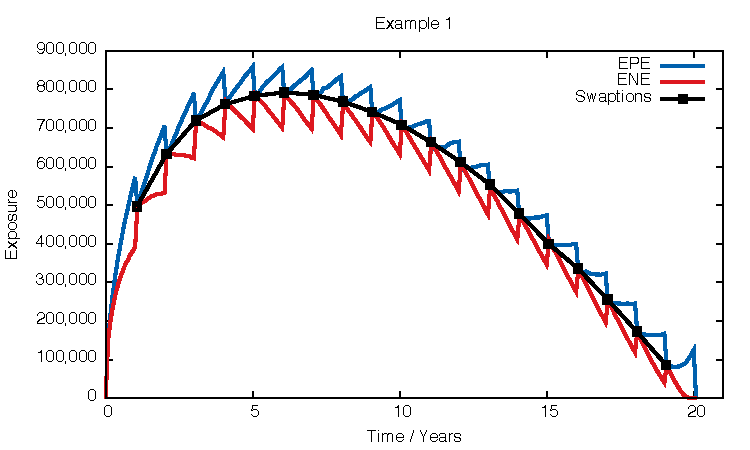
\includegraphics[scale=1.0]{example_swap_1.pdf}
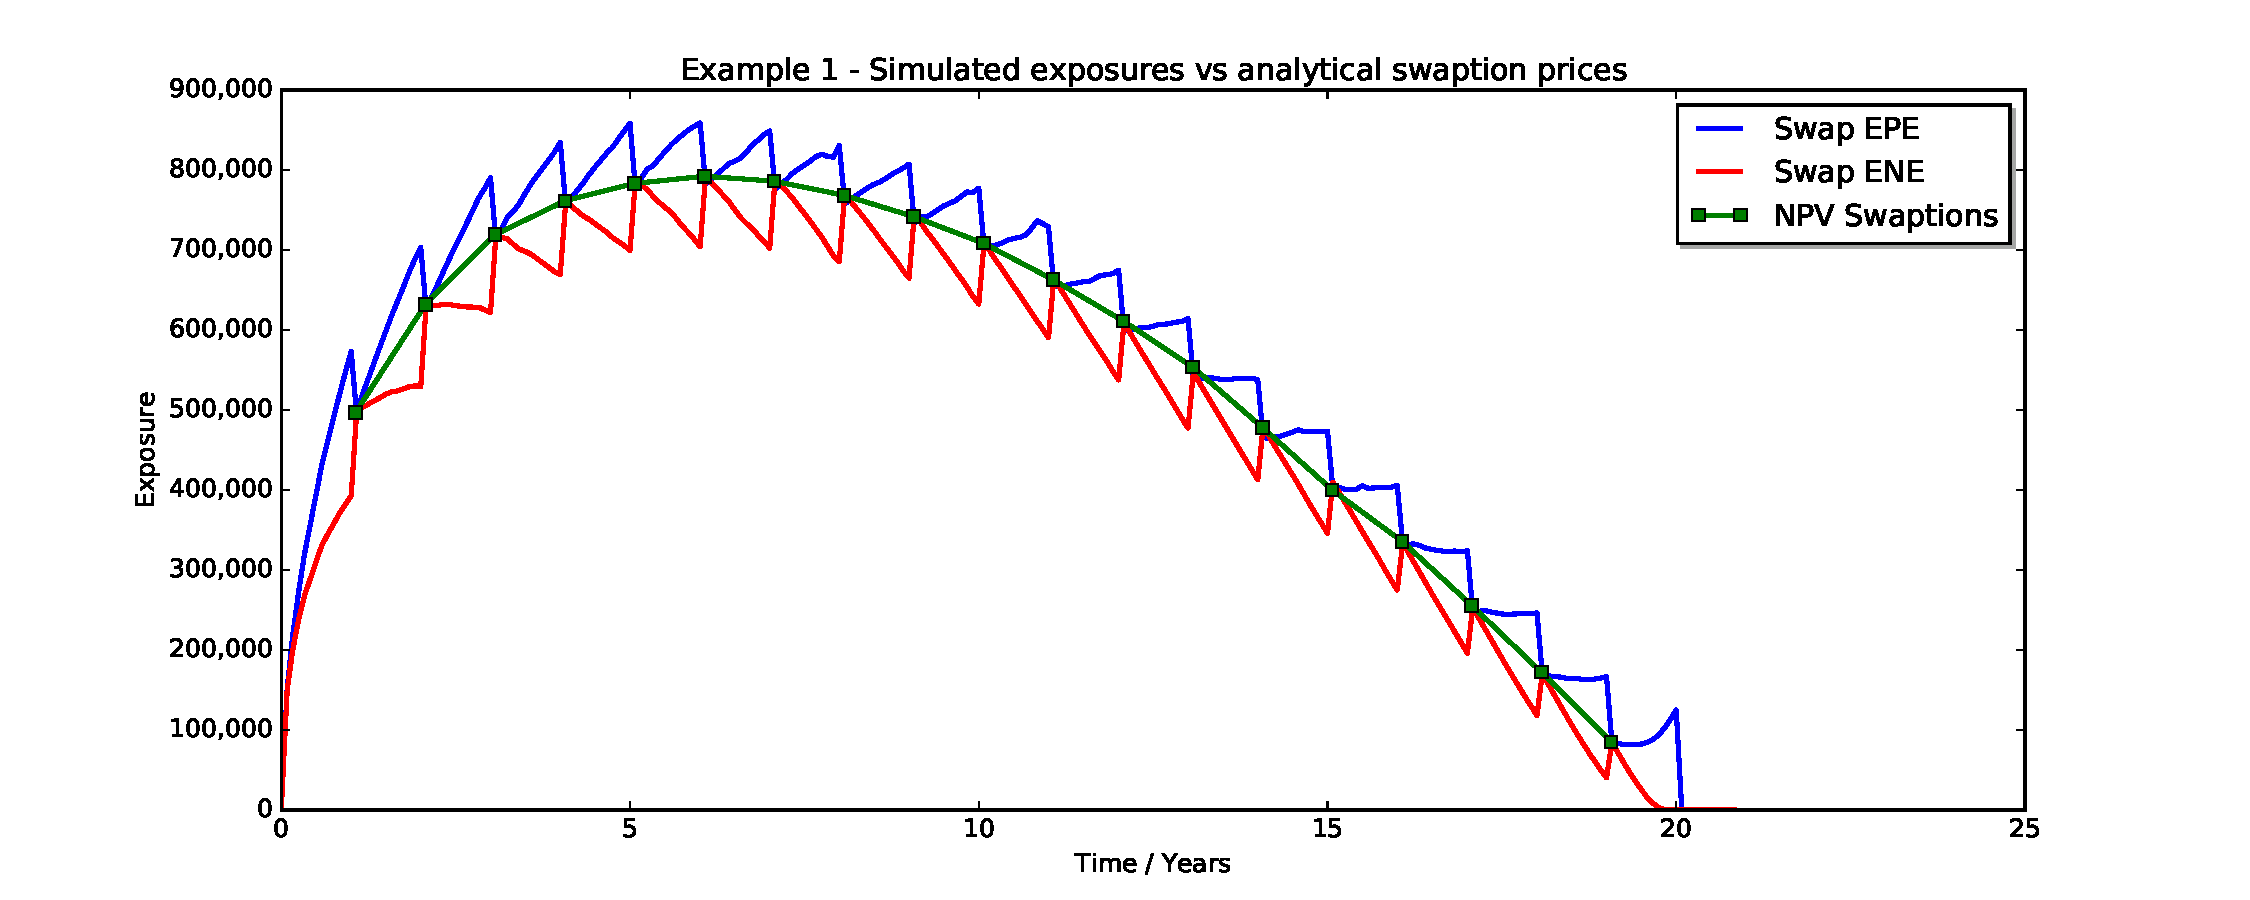
\includegraphics[scale=0.45]{mpl_swap_1.pdf}
\end{center}
\caption{Vanilla ATM swap expected exposure in a flat market environment from both parties' perspectives. The symbols are European Swaption prices. Simulation with 5000 paths and monthly time steps.}
\label{fig_1}
\end{figure}
The symbols are prices of European Swaptions with expiry at the symbol's time and otherwise same underlying as the Swap considered here. Both Swap simulation and Swaption pricing are run with calls to the ORE executable, essentially 

\medskip
\centerline{\tt ore[.exe] ore.xml} 

\centerline{\tt ore[.exe] ore\_swaption.xml} 
\medskip

which are wrapped into the script {\tt Examples/Example\_1/run.sh} provided with the ORE release.
It is instructive to look into the input folder in Examples/Example\_1, the content of the main input file {\tt ore.xml}, together with the explanations in section \ref{sec:configuration}.

\medskip
Moving to {\tt Examples/Example\_4}, we see what changes when using a realistic (non-flat) market environment as of 26/02/2016. Running the example with

\medskip
\centerline{\tt ./run.py } 
\medskip

yields the exposure evolution in 

\medskip
\centerline{\tt Examples/Example\_4/Output/*.pdf } 
\medskip

shown in figure \ref{fig_2}.
\begin{figure}[tb]
\begin{center}
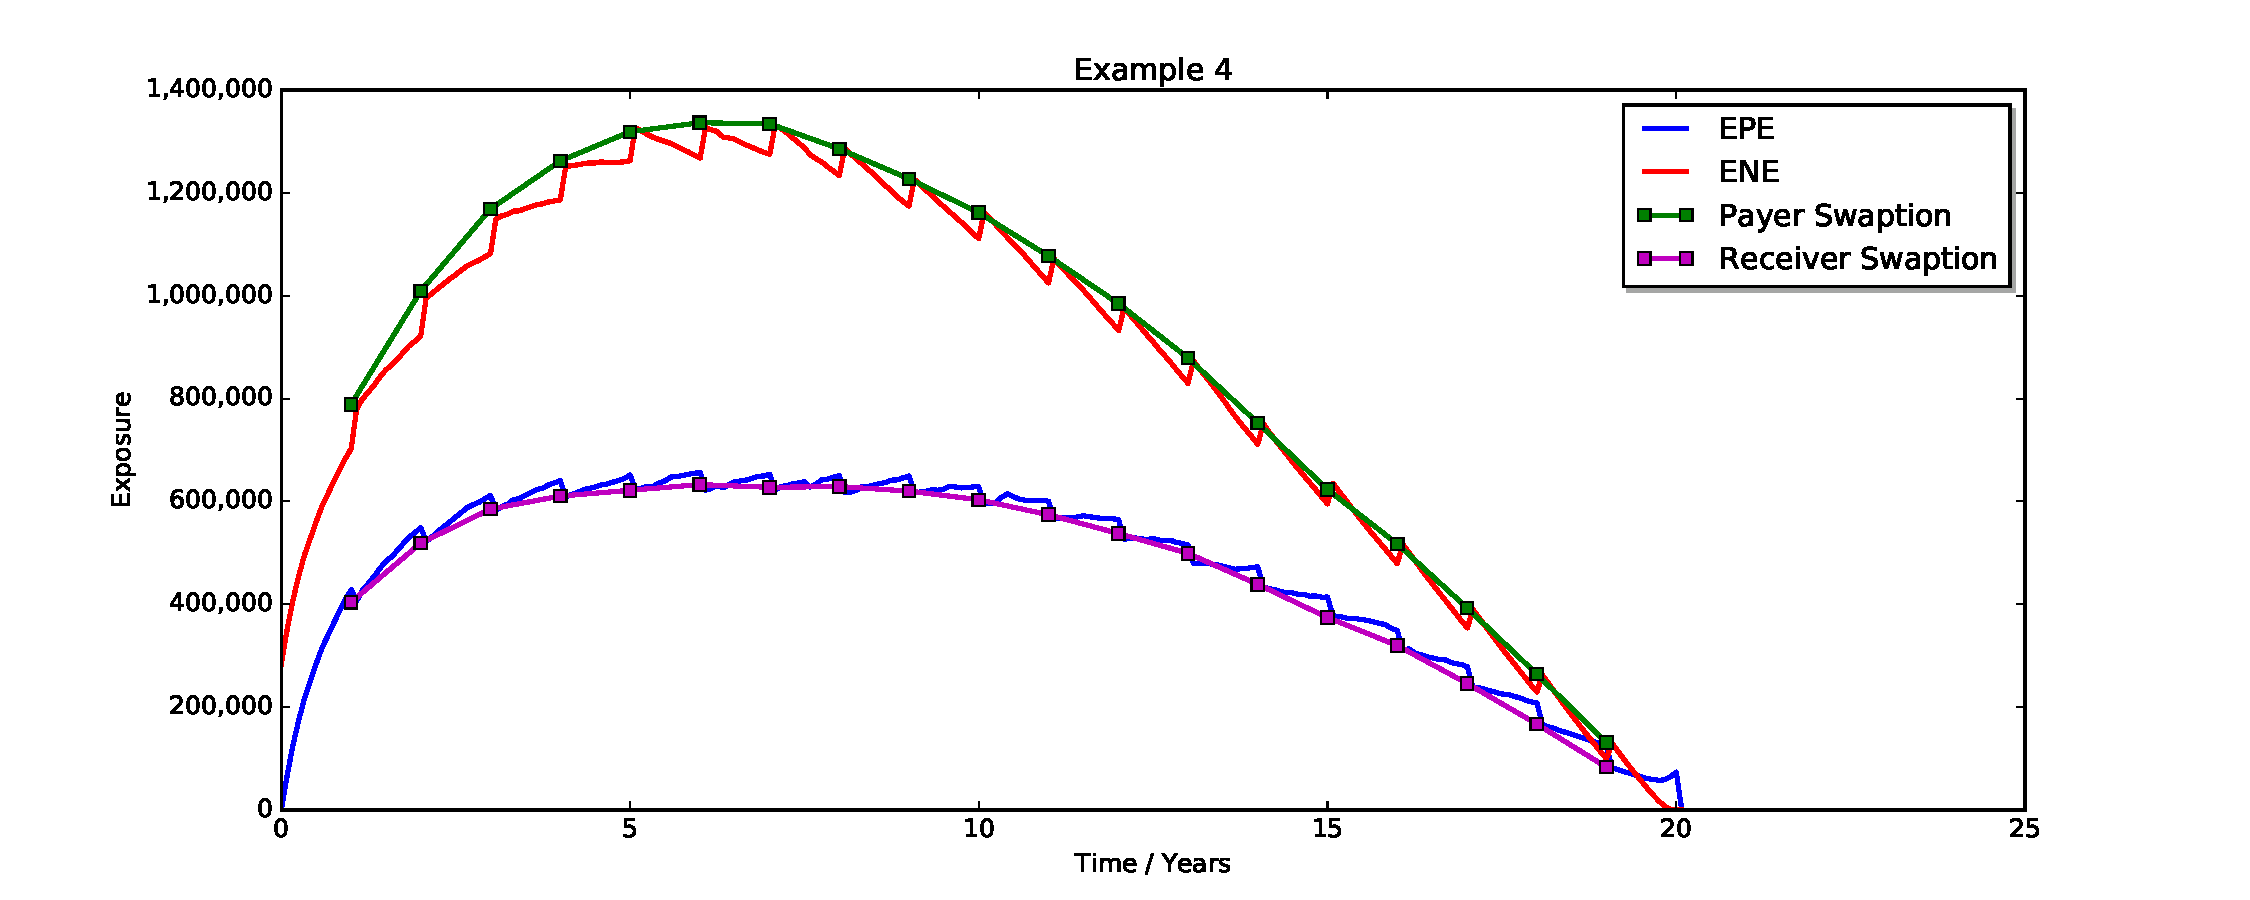
\includegraphics[scale=0.45]{mpl_swap_3.pdf}
%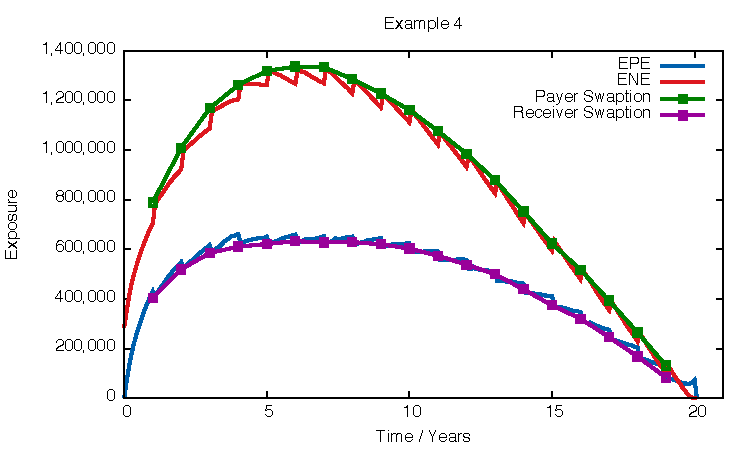
\includegraphics[scale=1.0]{example_swap_3.pdf}
\end{center}
\caption{Vanilla ATM swap expected exposure in a realistic market environment as of 26/02/2016 from both parties' perspectives. The Swap is the same as in figure \ref{fig_1} but receiving fixed 1\%, at the money on 26/02/2016. The symbols are the prices of European payer and receiver Swaptions. Simulation with 5000 paths and monthly time steps.}
\label{fig_2}
\end{figure}
In this case, where the curves (discount and forward) are upward sloping, the receiver swap is at the money at inception only and moves (on average) out of the money during its life. Similarly, the swap moves into the money from the counterparty's perspective. Hence the expected exposure evolutions from our perspective (EPE) and the counterparty's perspective (ENE) 'detach' here, while both can still be be reconciled with payer respectively receiver Swaption prices.

%--------------------------------------------------------
\subsection{European Swaption Exposure}\label{sec:european_swaption}
%--------------------------------------------------------

This demo case in folder {\tt Examples/Example\_7} shows the exposure evolution of European Swaptions with cash and physical delivery, respectively, see figure \ref{fig_3}.
\begin{figure}[hbt]
\begin{center}
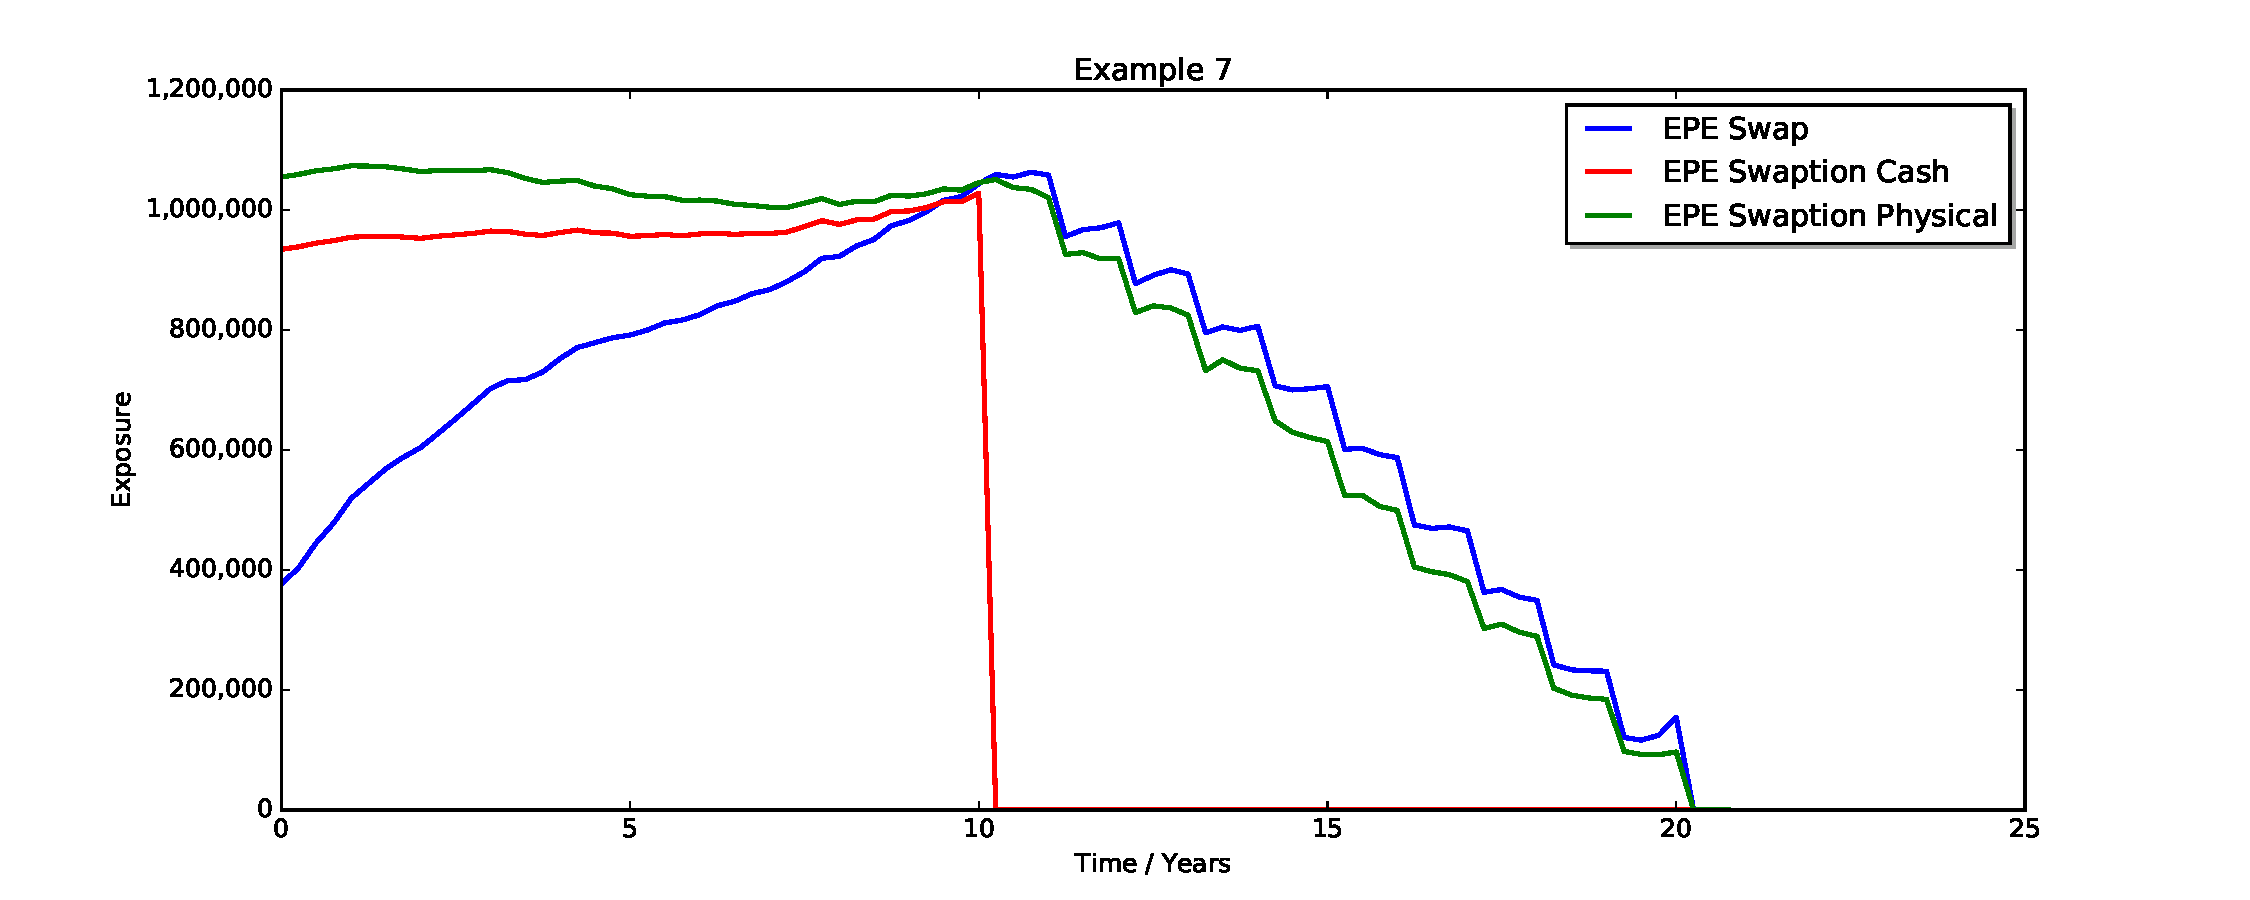
\includegraphics[scale=0.45]{mpl_swaption.pdf}
%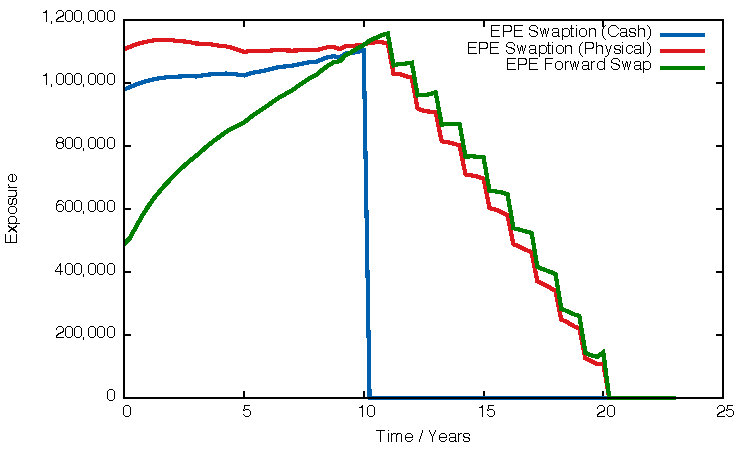
\includegraphics[scale=1.0]{example_swaption.pdf}
\end{center}
\caption{European Swaption exposure evolution, expiry in 10 years, final maturity in 20 years, for cash and physical delivery. Simulation with 1000 paths and quarterly time steps.}
\label{fig_3}
\end{figure}
The delivery type (cash vs physical) yields significantly different valuations as of today due to the steepness of the relevant yield curves (EUR). The cash settled Swaption's exposure graph is truncated at the exercise date, whereas the physically settled Swaption exposure turns into a Swap-like exposure after expiry. For comparison, the example also provides the exposure evolution of the underlying forward starting Swap which yields a somewhat higher exposure after the forward start date than the physically settled Swaption. This is due to scenarios with negative swap NPV at expiry and positive NPVs thereafter.

%--------------------------------------------------------
\subsection{Bermudan Swaption Exposure}
%--------------------------------------------------------

This demo case in folder {\tt Examples/Example\_10} shows the exposure evolution of Bermudan rather than European Swaptions with cash and physical delivery, respectively, see figure \ref{fig_3b}.
\begin{figure}[hbt]
\begin{center}
%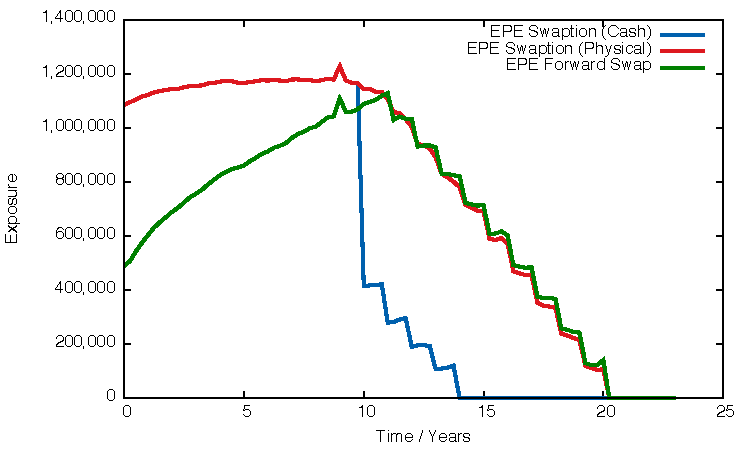
\includegraphics[scale=1.0]{example_bermudan_swaption.pdf}
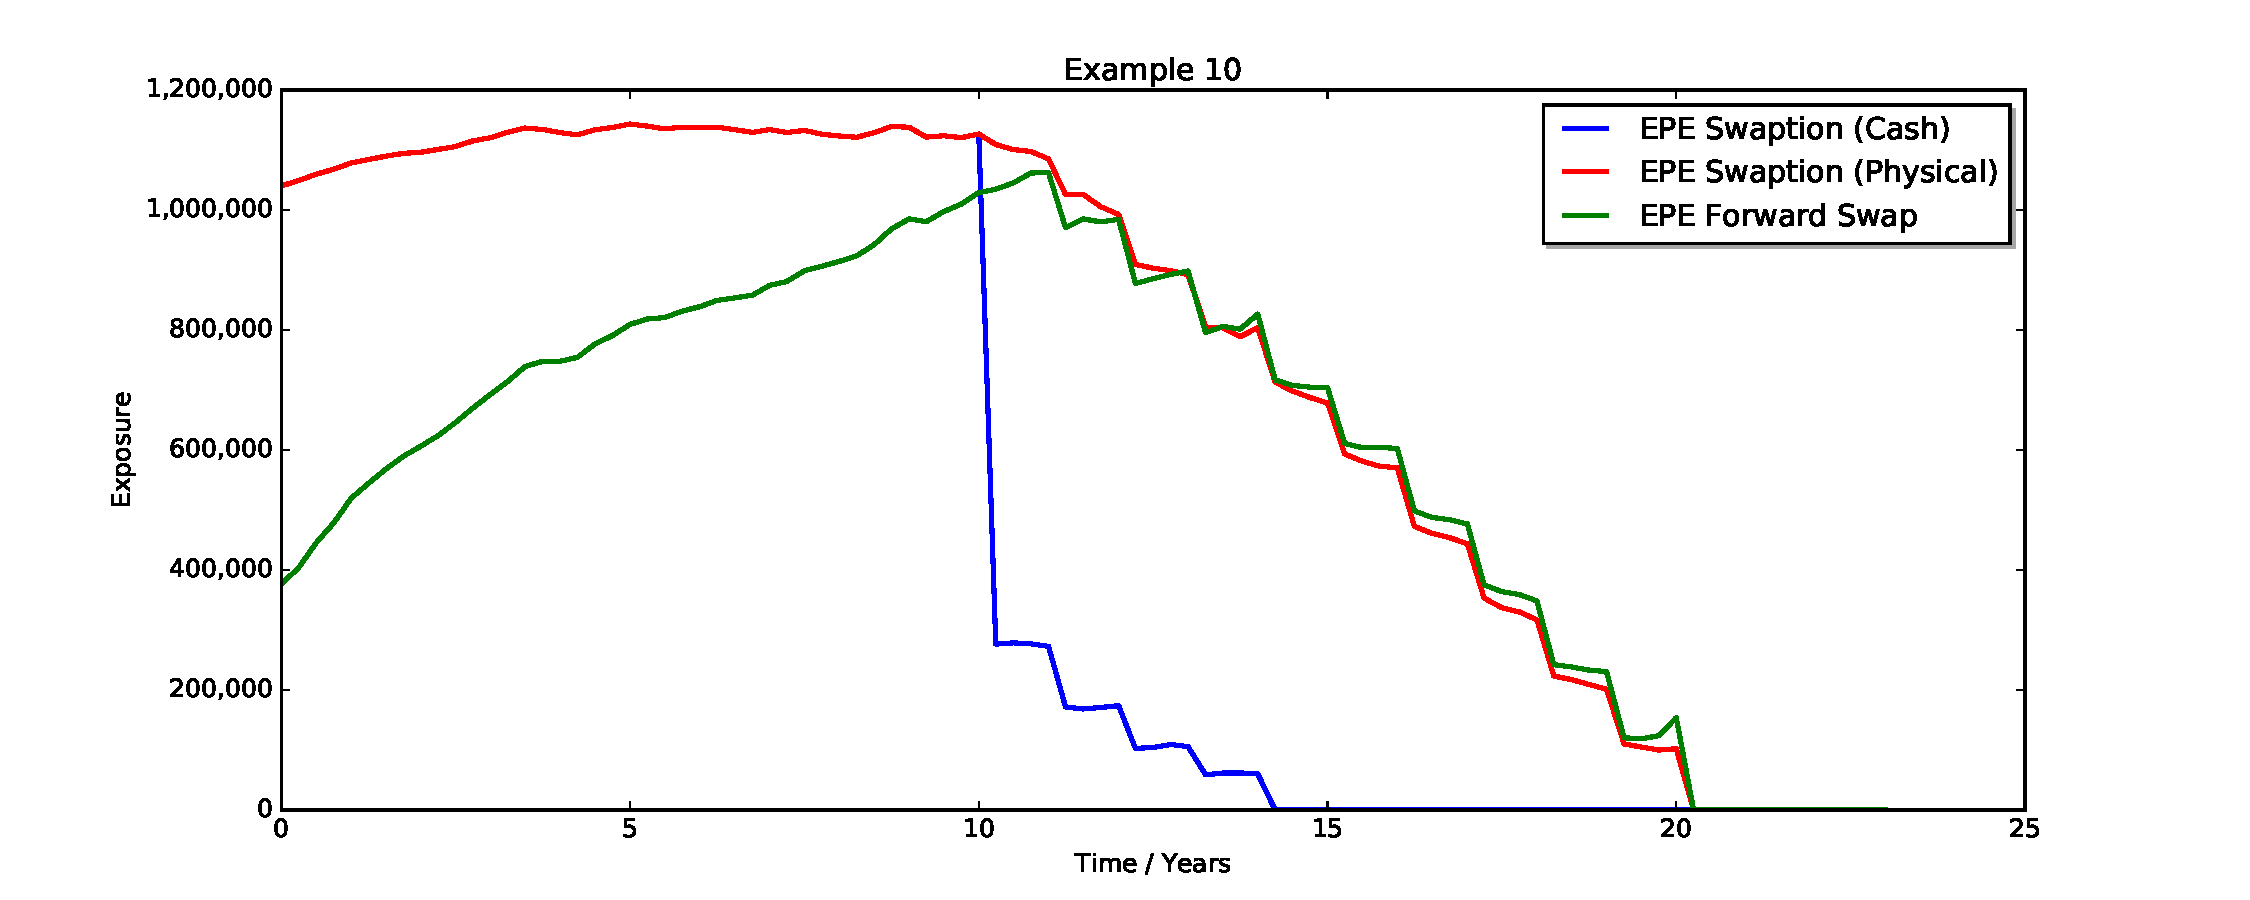
\includegraphics[scale=0.45]{mpl_bermudan_swaption.pdf}
\end{center}
\caption{Bermudan Swaption exposure evolution, 5 annual exercise dates starting in 10 years, final maturity in 20 years, for cash and physical delivery. Simulation with 1000 paths and quarterly time steps.}
\label{fig_3b}
\end{figure}
The underlying Swap is the same as in the European Swaption example in section \ref{sec:european_swaption}. Note in particular the difference between the Bermudan and European Swaption exposures with cash settlement: The Bermudan shows the typical step-wise decrease due to the series of exercise dates. Also note that we are using the same Bermudan option pricing engines for both settlement types, in contrast to the European case, so that the Bermudan option cash and physical exposures are identical up to the first exercise date. When running this example, you will notice the significant difference in computation time compared to the European case (ballpark 30 minutes here for 2 Swaptions, 1000 samples, 90 time steps). The Bermudan example is way slower because we use an LGM grid engine for pricing under scenarios in this case. In a realistic context one would more likely resort to American Monte Carlo simulation, feasible in ORE, but not provided in the first release. However, this implementation can be used to benchmark any faster / more sophisticated approach to Bermudan Swaption exposure simulation.

%--------------------------------------------------------
\subsection{Callable Swap Exposure}
%--------------------------------------------------------

This demo case in folder {\tt Examples/Example\_6} shows the exposure evolution of a European callable Swap, represented as two trades - the non-callable Swap and a Swaption with physical delivery. We have sold the call option, i.e. the Swaption is a right for the counterparty to enter into an offsetting Swap which economically terminates all future flows if exercised. The resulting exposure evolutions for the individual components (Swap, Swaption), as well as the callable Swap are shown in figure \ref{fig_4}. 
\begin{figure}[hbt]
\begin{center}
%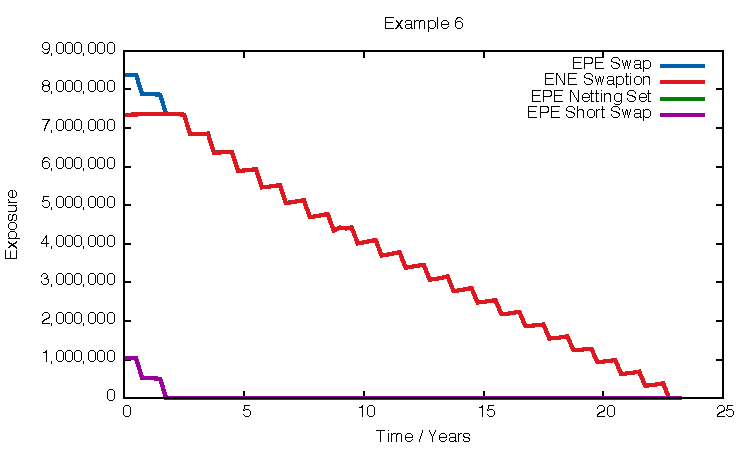
\includegraphics[scale=1.0]{example_callable_swap.pdf}
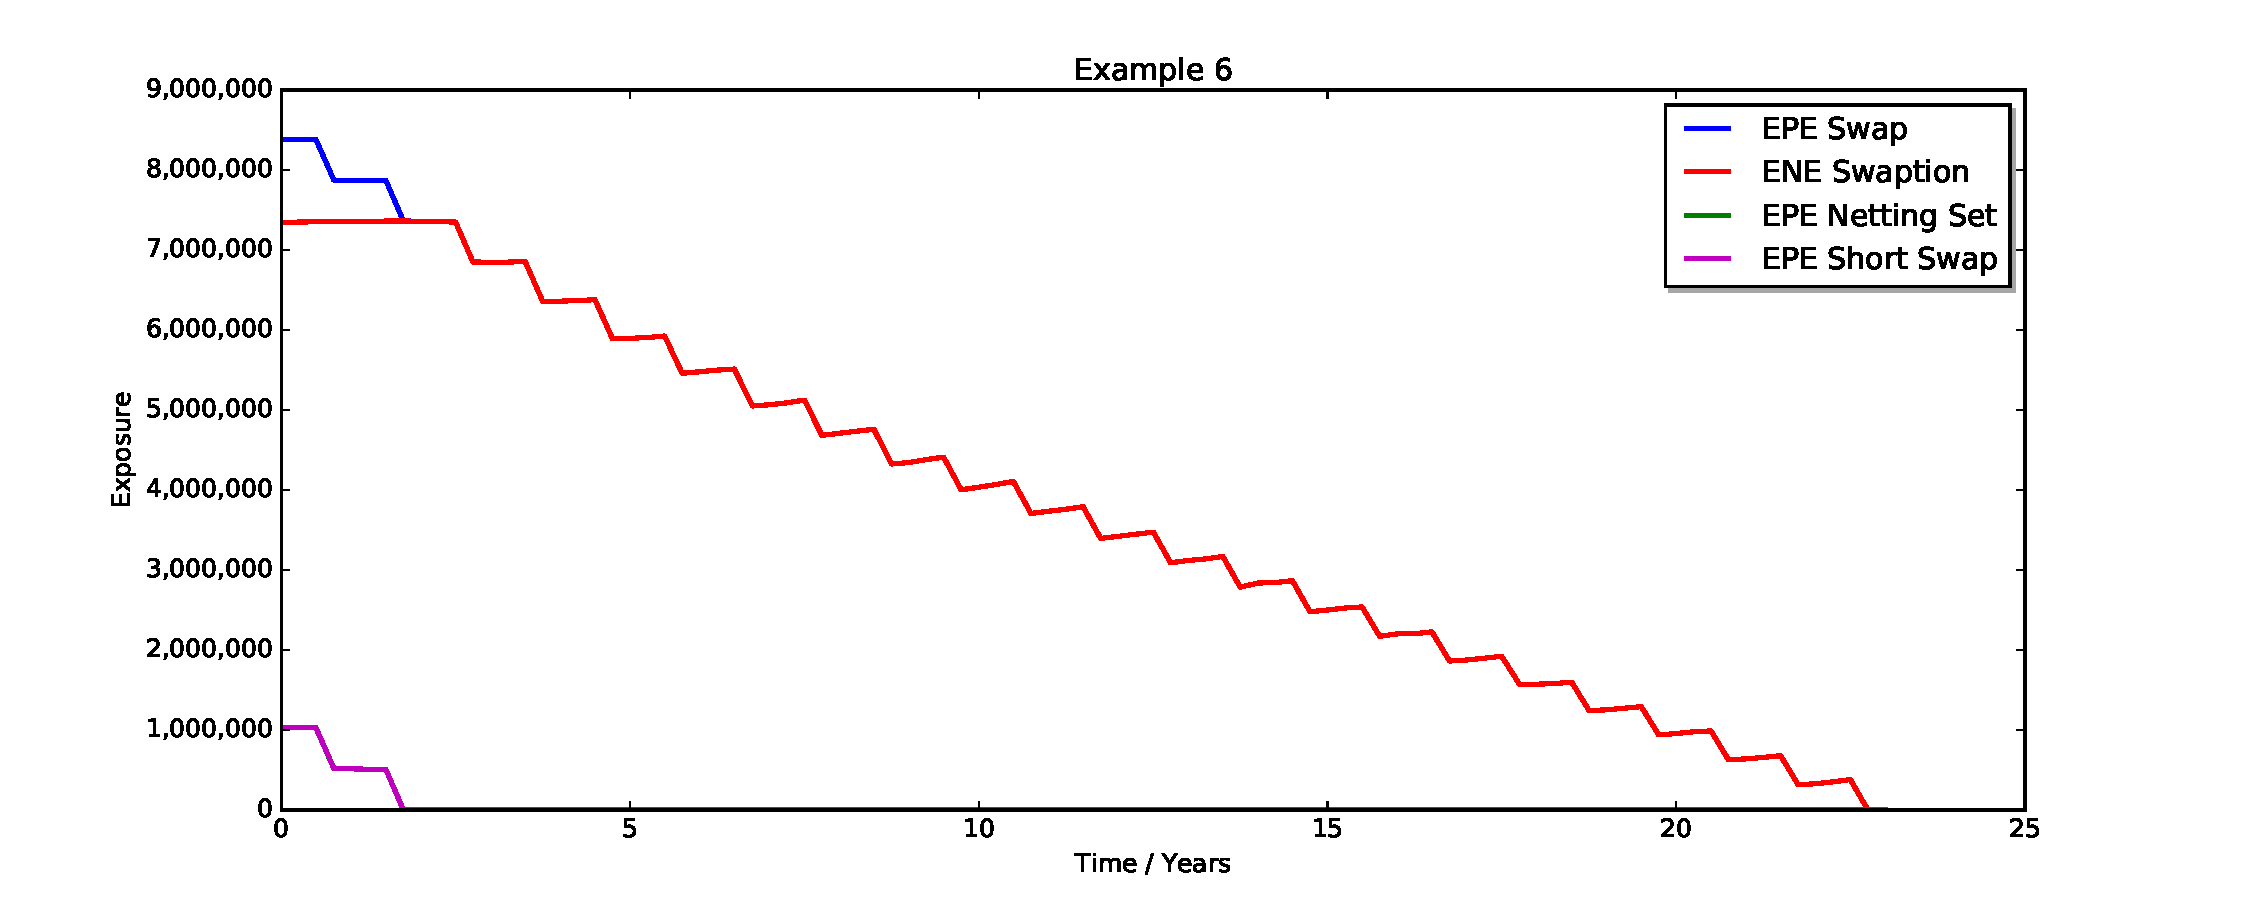
\includegraphics[scale=0.45]{mpl_callable_swap.pdf}
\end{center}
\caption{European callable Swap represented as a package consisiting of non-callable Swap and Swaption. The Swaption has physical delivery and offsets all future Swap cash flows if exercised. The exposure evolution of the package is shown here as 'EPE NettingSet' (green line). This is covered by the pink line, the exposure evolution of the same Swap but with maturity on the exercise date. The graphs match perfectly here, because the example Swap is deep in the money and exercise probability is close to one. Simulation with 5000 paths and quarterly time steps.}
\label{fig_4}
\end{figure}
The example is an extreme case where the underlying Swap is deeply in the money (receiving fixed 5\%), and hence the call exercise probability is close to one. Modify the Swap and Swaption fixed rates closer to the money ($\approx$ 1\%) to see the deviation between net exposure of the callable Swap and the exposure of a 'short' Swap with maturity on exercise.  

%--------------------------------------------------------
\subsection{Cap/Floor Exposure}\label{sec:capfloor}
%--------------------------------------------------------

The example in folder {\tt Examples/Example\_12} generates exposure evolutions of several swaps, caps and floors. The example shown in figure \ref{fig_capfloor_1} ('portfolio 1') consists of a 20y Swap receiving 1\% fixed and a 20y Collar with both cap and floor at 2.5\% so that the net exposure corresponds to a Swap receiving 0.5\% fixed.

\begin{figure}[hbt]
\begin{center}
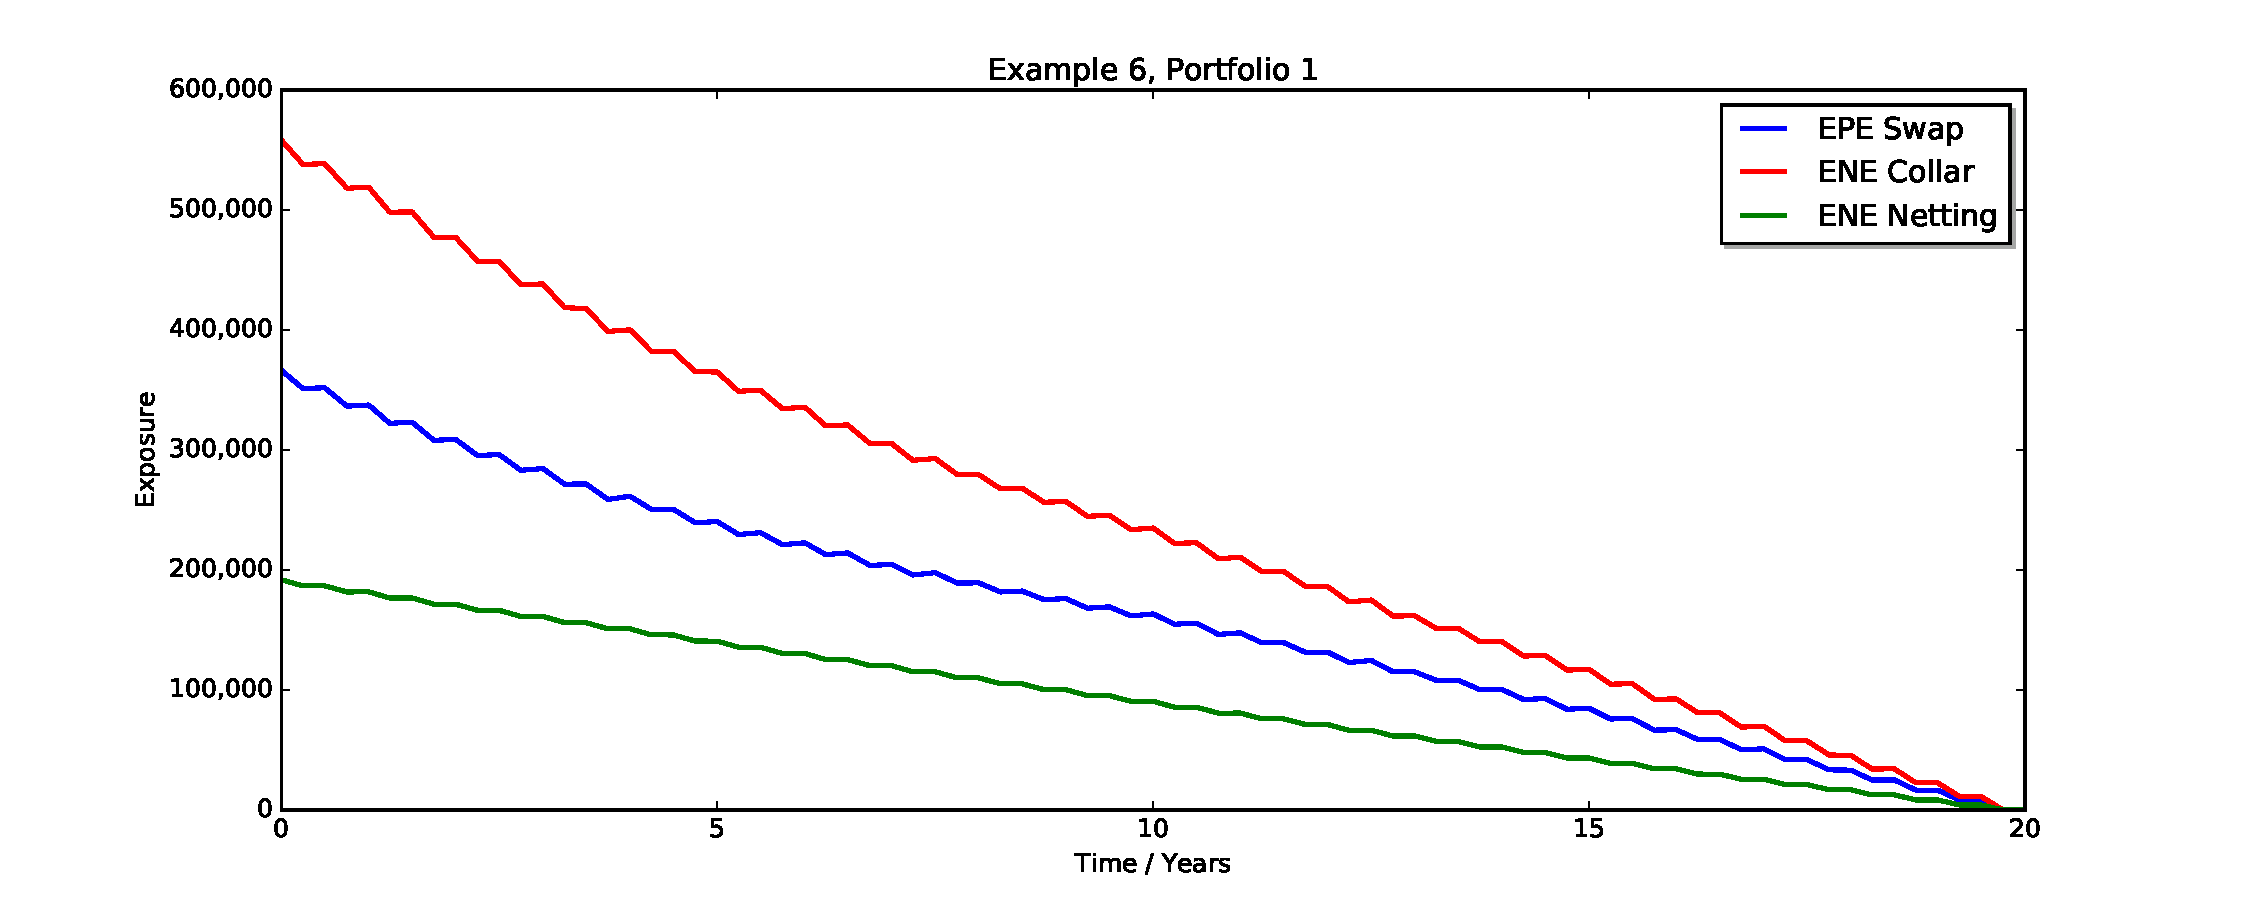
\includegraphics[scale=0.45]{mpl_capfloor_1.pdf}
\end{center}
\caption{Swap+Collar, portfolio 1. The Collar has identical cap and floor rates at 2.5\% so that it corresponds to a fixed leg which reduces the exposure of the Swap, which receives 3\% fixed. Simulation with 1000 paths and quarterly time steps.}
\label{fig_capfloor_1}
\end{figure}

The second example in this folder shown in figure \ref{fig_capfloor_2} ('portfolio 2') consists of a short Cap, long Floor and a Collar that corresponds to the netted Cap and Floor.

\begin{figure}[hbt]
\begin{center}
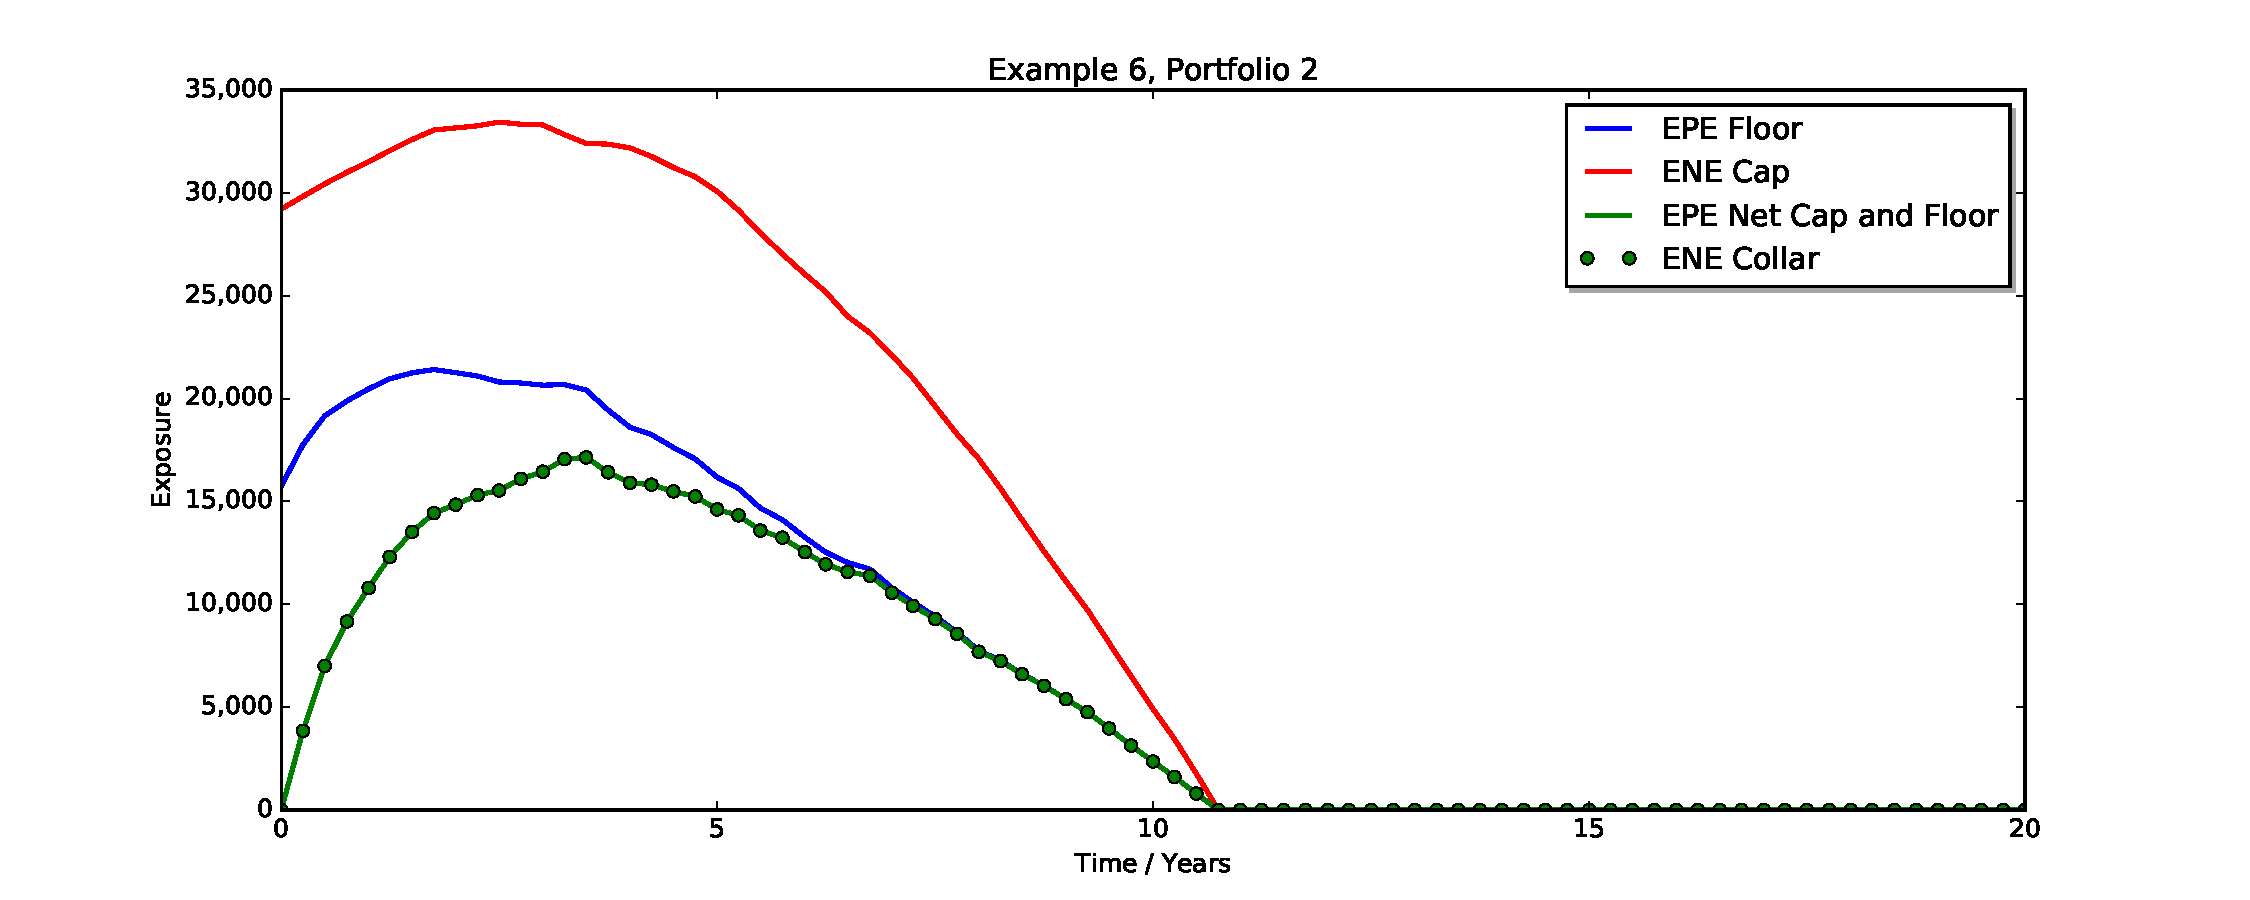
\includegraphics[scale=0.45]{mpl_capfloor_2.pdf}
\end{center}
\caption{Short Cap and long Floor vs Collar, portfolio 2. Simulation with 1000 paths and quarterly time steps.}
\label{fig_capfloor_2}
\end{figure}
 
%--------------------------------------------------------
\subsection{FX Forward Exposure}\label{sec:fxfwd}
%--------------------------------------------------------

The example in folder {\tt Examples/Example\_2} generates the exposure evolution for a EUR / USD FX Forward transaction with value date in 10Y. This is a particularly simple show case because of the single cash flow in 10Y. On the other hand it checks the cross currency model implementation by means of comparison to analytic limits - EPE and ENE at the trade's value date must match corresponding Vanilla FX Option prices, as shown in figure \ref{fig_5}.  
\begin{figure}[hbt]
\begin{center}
%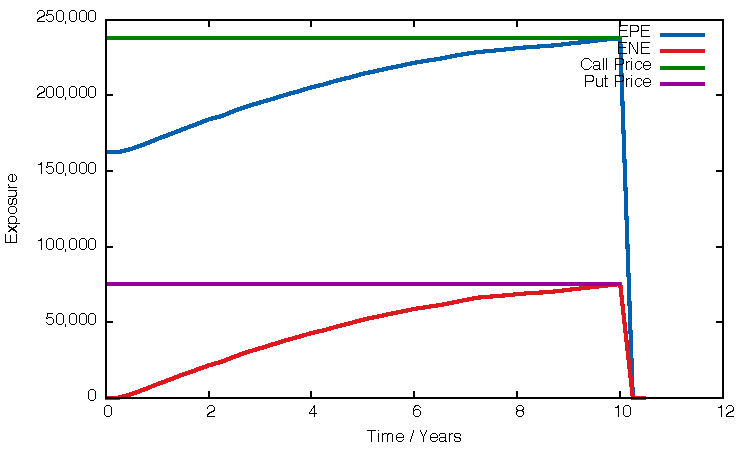
\includegraphics[scale=1.0]{example_fxforward.pdf}
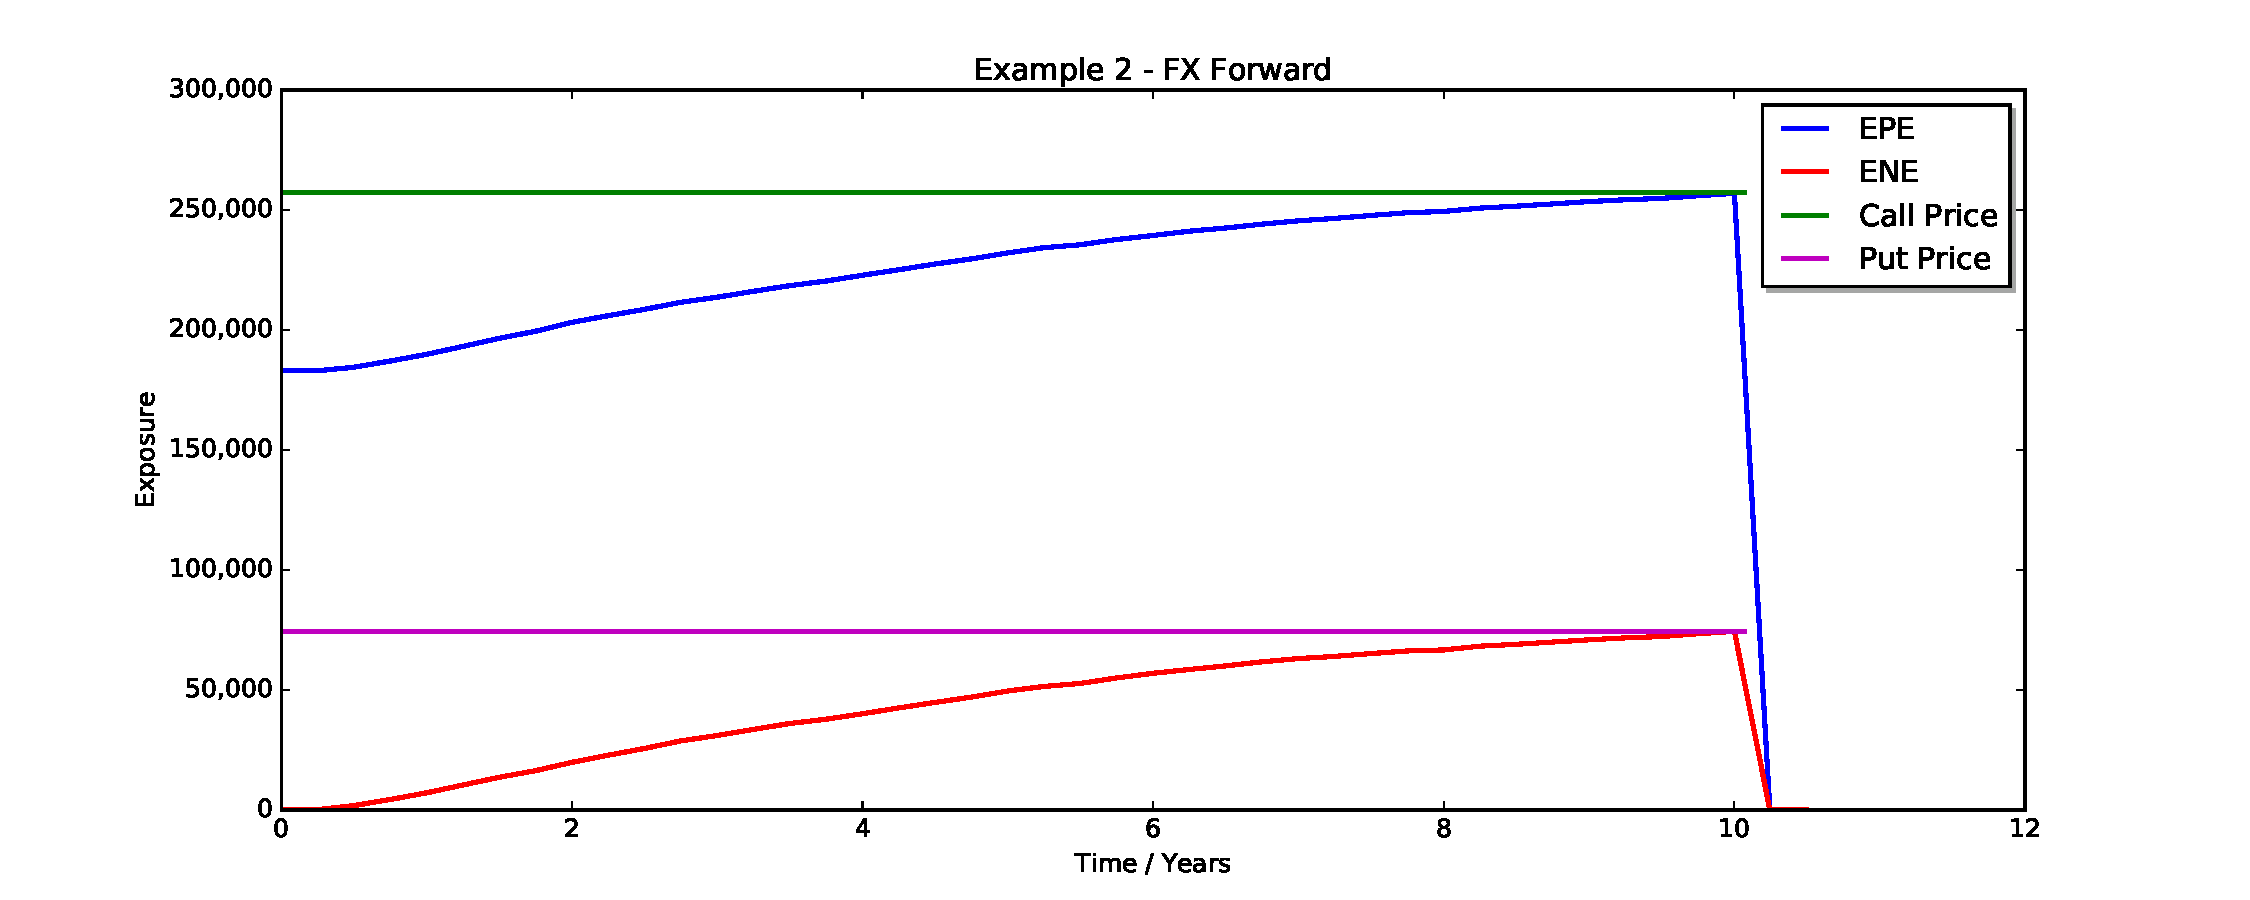
\includegraphics[scale=0.45]{mpl_fxforward.pdf}
\end{center}
\caption{EUR/USD FX Forward expected exposure in a realistic market environment as of 26/02/2016 from both parties' perspectives. Value date is obviously in 10Y. The flat lines are FX Option prices which coincide with EPE and ENE, respectively, on the value date. Simulation with 5000 paths and quarterly time steps.}
\label{fig_5}
\end{figure}

%--------------------------------------------------------
\subsection{Cross Currency Swap Exposure and FX Reset}
%--------------------------------------------------------

The case in {\tt Examples/Example\_8} is a vanilla cross currency swap. It shows the typical blend of and interest rate swap's saw tooth exposure evolution with an FX forward's exposure which increases monotonically to final maturity, see figure \ref{fig_6}. 
%\todo[inline]{Done - Add notional resetting feature and example}
\begin{figure}[hbt]
\begin{center}
%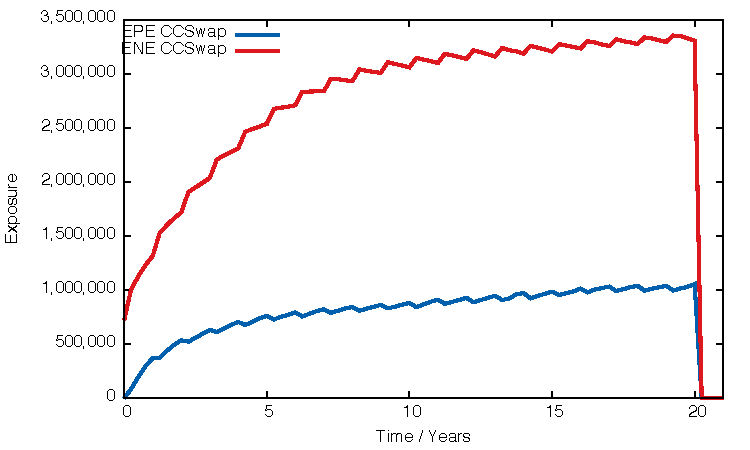
\includegraphics[scale=1.0]{example_ccswap.pdf}
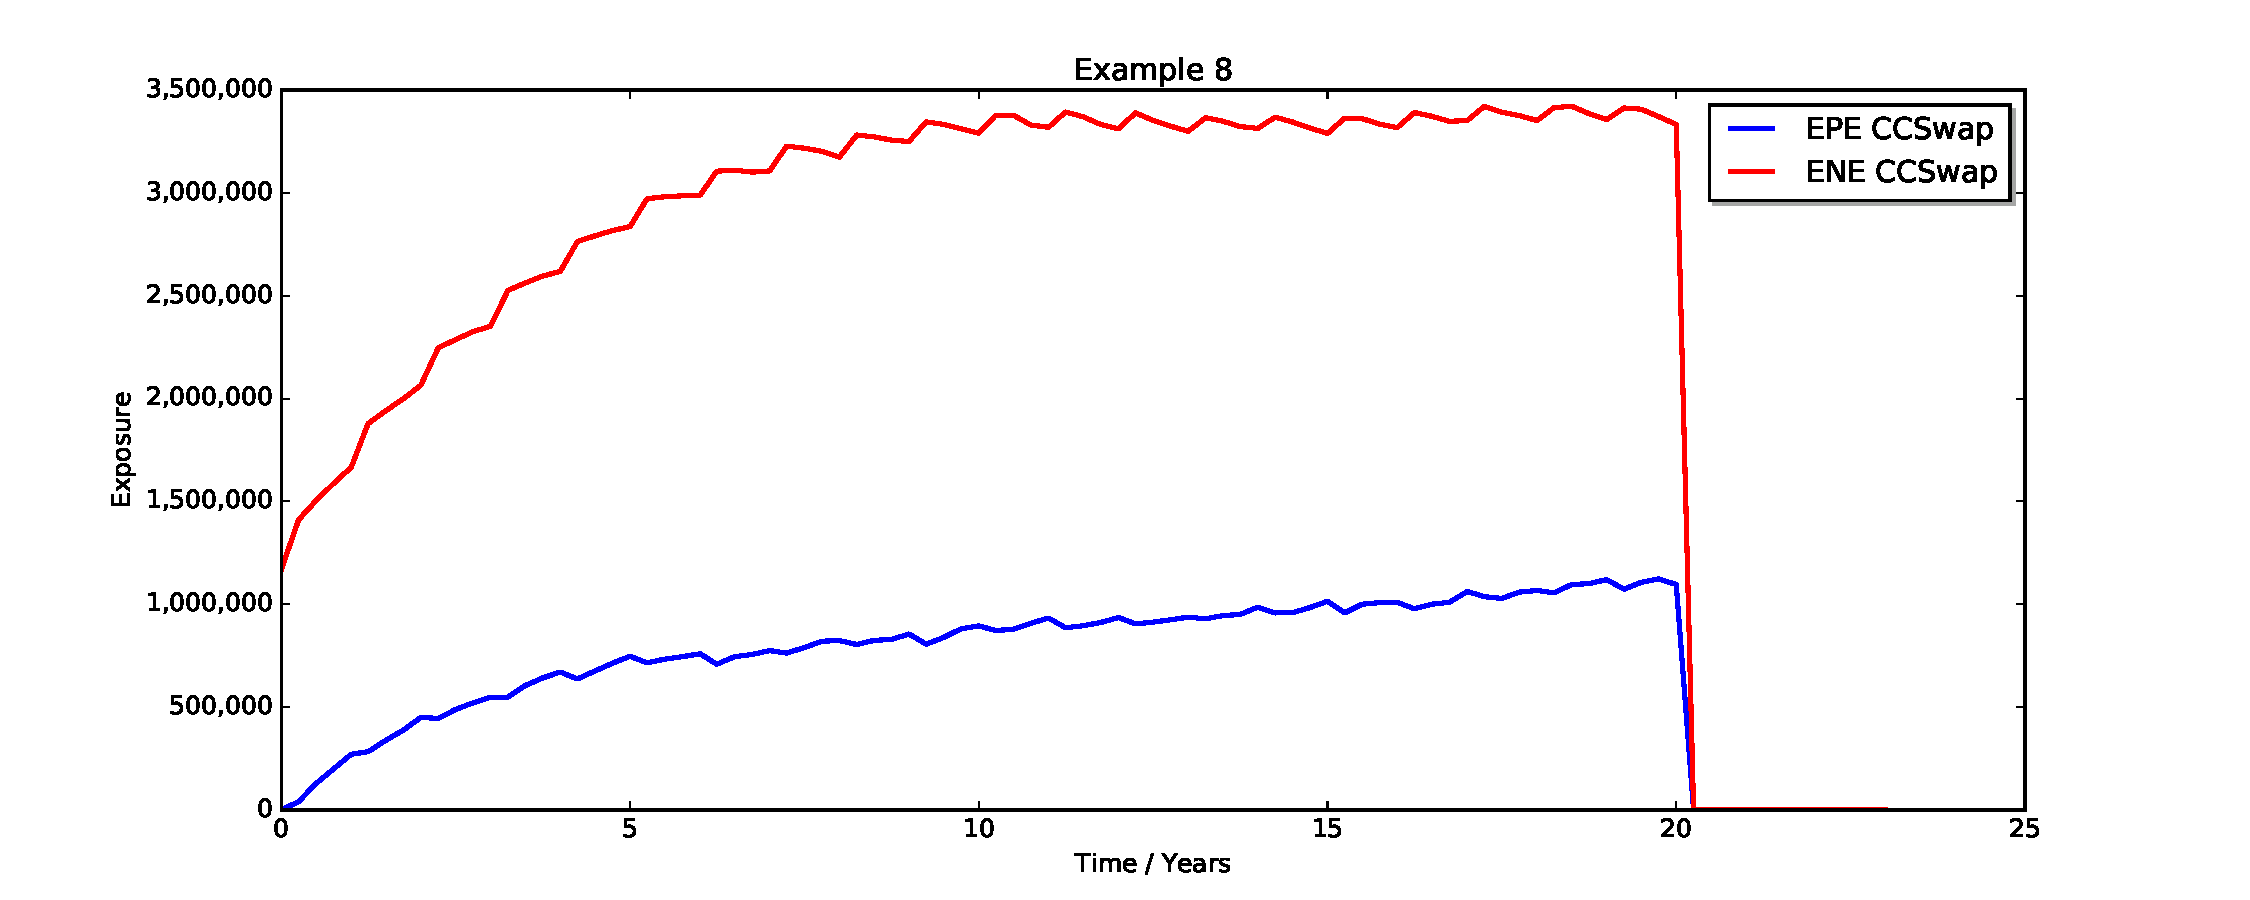
\includegraphics[scale=0.45]{mpl_ccswap.pdf}
\end{center}
\caption{Cross Currency Swap exposure evolution without mark-to-market notional reset. Simulation with 1000 paths and quarterly time steps.}
\label{fig_6}
\end{figure}
The case in {\tt Examples/Example\_9} then shows the effect of FX resets in a EUR/USD cross currency basis swap, see figure \ref{fig_6b}. As expected, the notional reset causes an exposure collapse at each period start when the EUR leg's notional is reset to match the USD notional.
\begin{figure}[hbt]
\begin{center}
%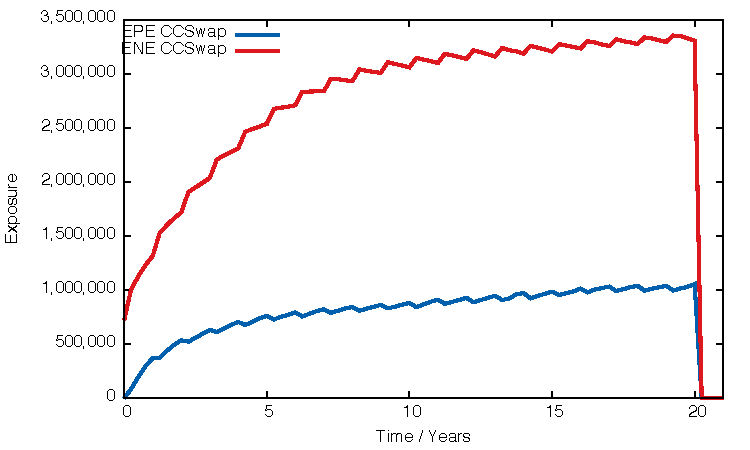
\includegraphics[scale=1.0]{example_ccswap.pdf}
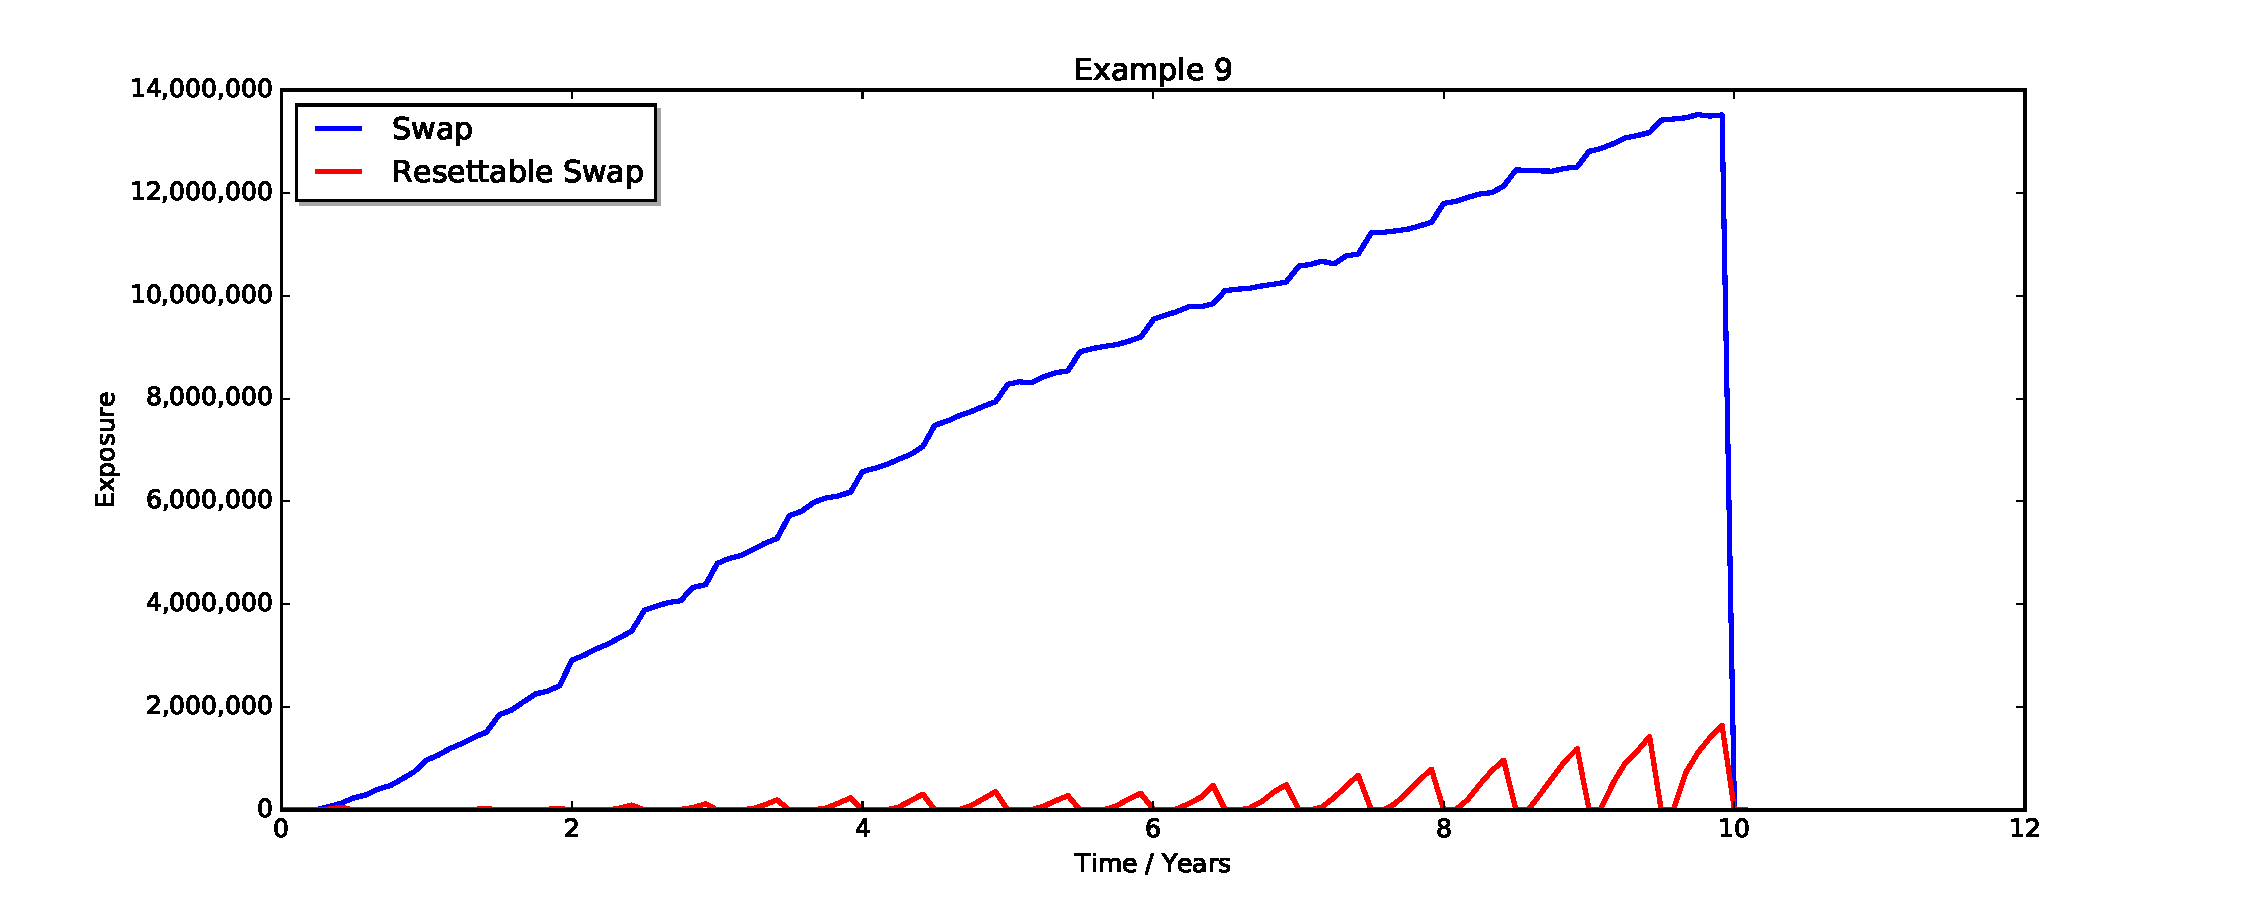
\includegraphics[scale=0.45]{mpl_xccy_reset.pdf}
\end{center}
\caption{Cross Currency Basis Swap exposure evolution with and without mark-to-market notional reset. Simulation with 1000 paths and quarterly time steps.}
\label{fig_6b}
\end{figure}
  
%--------------------------------------------------------
\subsection{FX Option Exposure}
%--------------------------------------------------------

This example (in folder {\tt Examples/Example\_2}, as the FX Forward example) illustrates the exposure evolution for an FX Option, see figure \ref{fig_7}. 
\begin{figure}[hbt]
\begin{center}
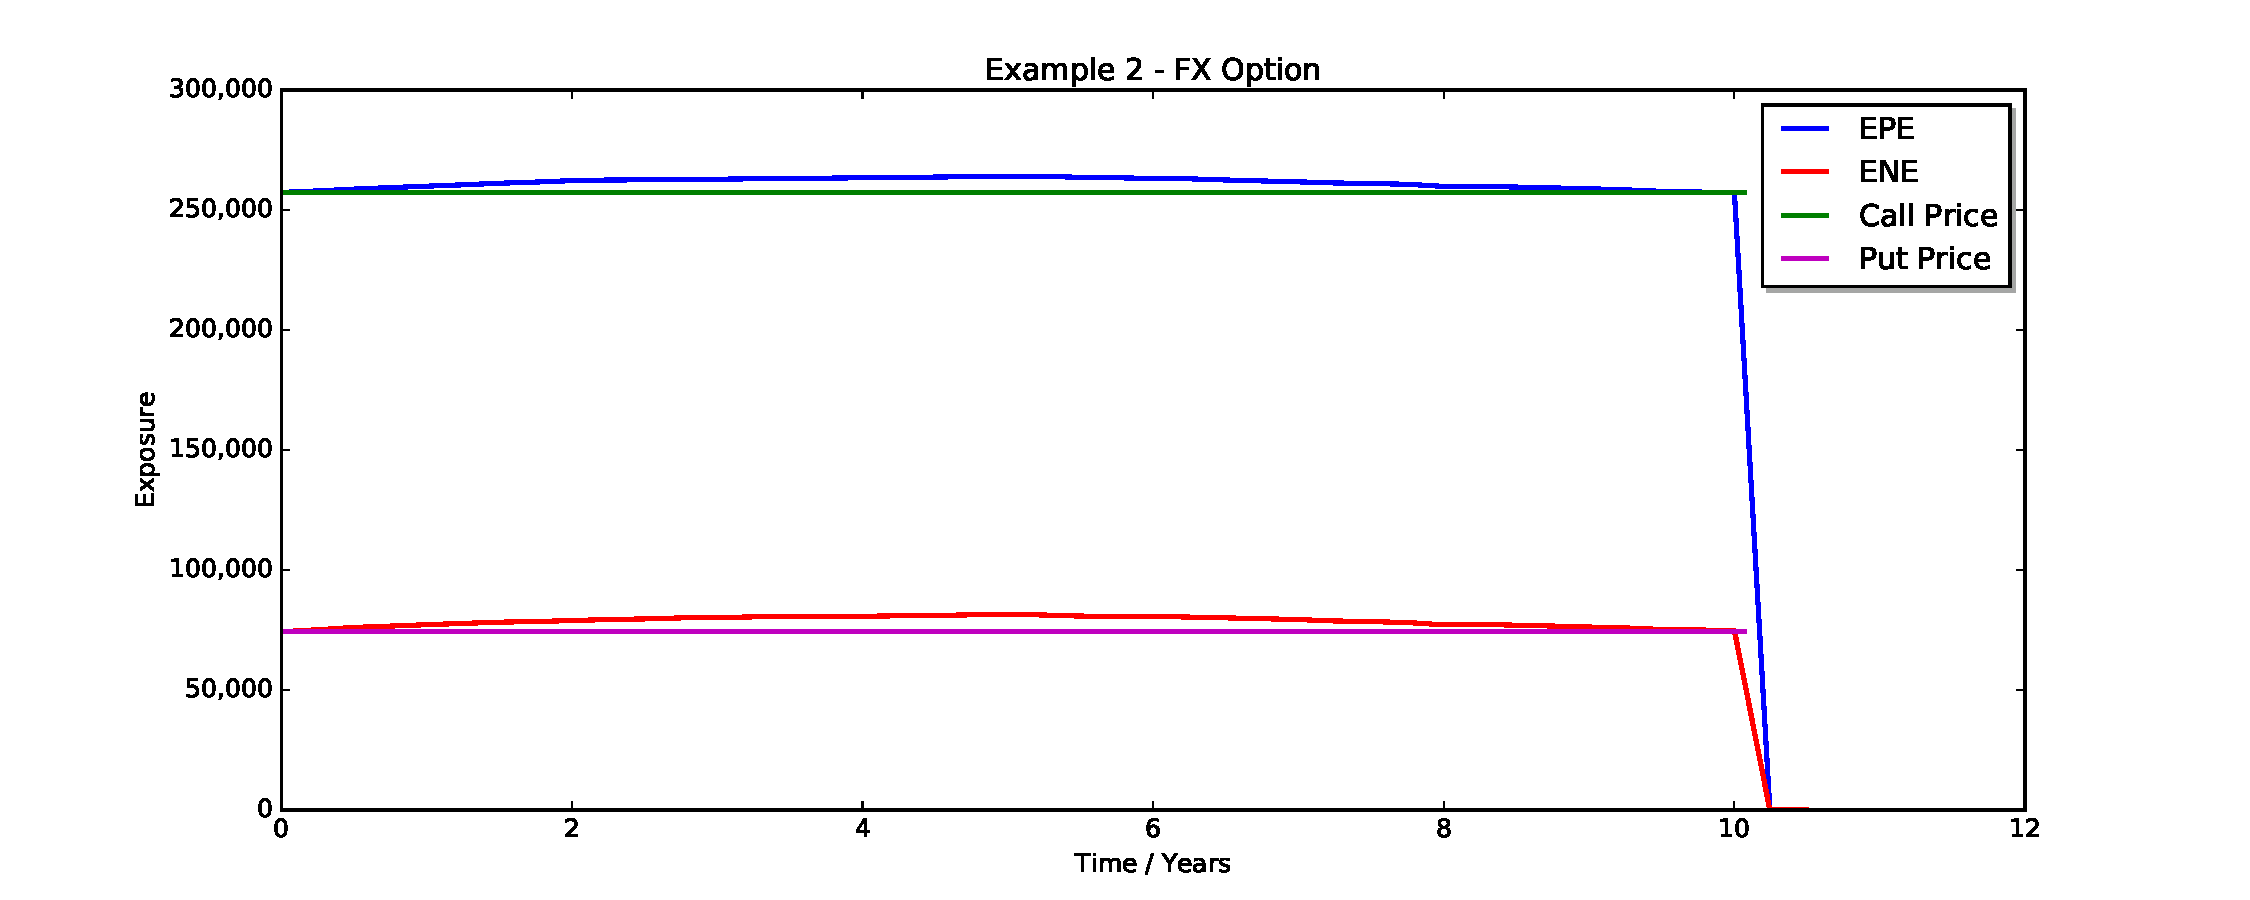
\includegraphics[scale=0.45]{mpl_fxoption.pdf}
%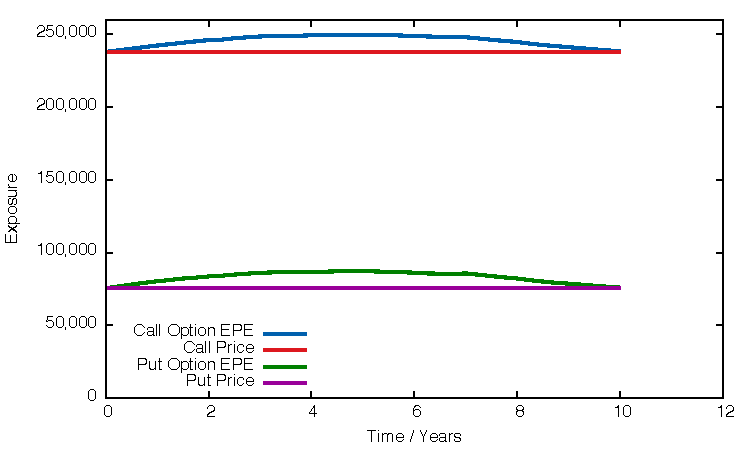
\includegraphics[scale=1.0]{example_fxoption_fwdvariance_corrected.pdf}
\end{center}
\caption{EUR/USD FX Call and Put Option exposure evolution, same underlying and market data as in section \ref{sec:fxfwd}, compared to the call and put option price as of today (flat line). Simulation with 5000 paths and quarterly time steps.}
\label{fig_7}
\end{figure}
Recall that the FX Option value $NPV(t)$ as of time $0 \leq t \leq T$ satisfies
\begin{align*}
\frac{NPV(t)}{N(t)} &= \mbox{Nominal}\times\E_t\left[\frac{(X(T) - K)^+}{N(T)}\right]\\
NPV(0) &= \E\left[\frac{NPV(t)}{N(t)}\right] = \E\left[\frac{NPV^+(t)}{N(t)} \right]= \EPE(t) 
\end{align*}
One would therefore expect a flat exposure evolution up to option expiry. The deviation from this in ORE's simulation is due to the pricing approach chosen here under scenarios. A Black FX option pricer is used with simulated interest rate curves input and {\em deterministic} Black volatility derived from today's volatility structure (pushed or rolled forward, see section \ref{sec:sim_market}). The deviation can be removed by extending the volatility modelling, e.g. implying model consistent Black volatilities in each simulation step on each path.
\todo[inline]{Add exposure evolution graph with 'simulated' FX vol}

%--------------------------------------------------------
\subsection{Netting and Collateral}
%--------------------------------------------------------

In this example (see folder {\tt Examples/Example\_5}) we showcase a small netting set consisting of three swaps in different currencies, with different collateral choices
\begin{itemize}
\item no collateral - figure \ref{fig_8},
\item collateral with threshold (THR) 1m EUR, minimum transfer amount (MTA) 100k EUR, margin period of risk (MPoR) 2 weeks - figure \ref{fig_9}
\item collateral with zero THR and MTA, and MPoR 2w - figure \ref{fig_10}
\end{itemize}
 
\begin{figure}[tb]
\begin{center}
%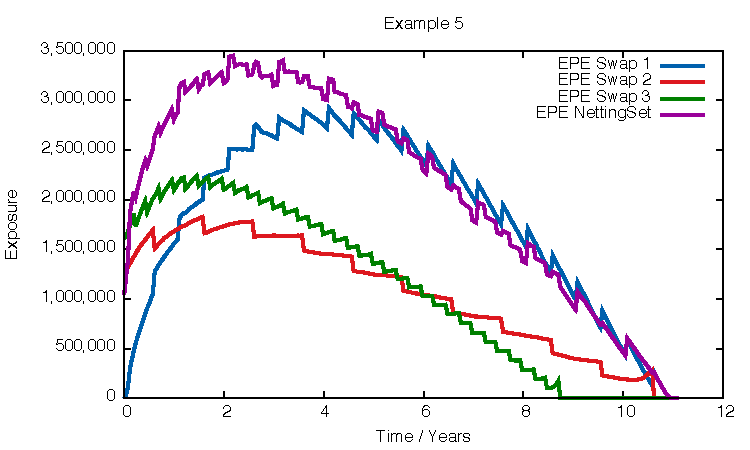
\includegraphics[scale=1.0]{example_nocollateral_epe.pdf}
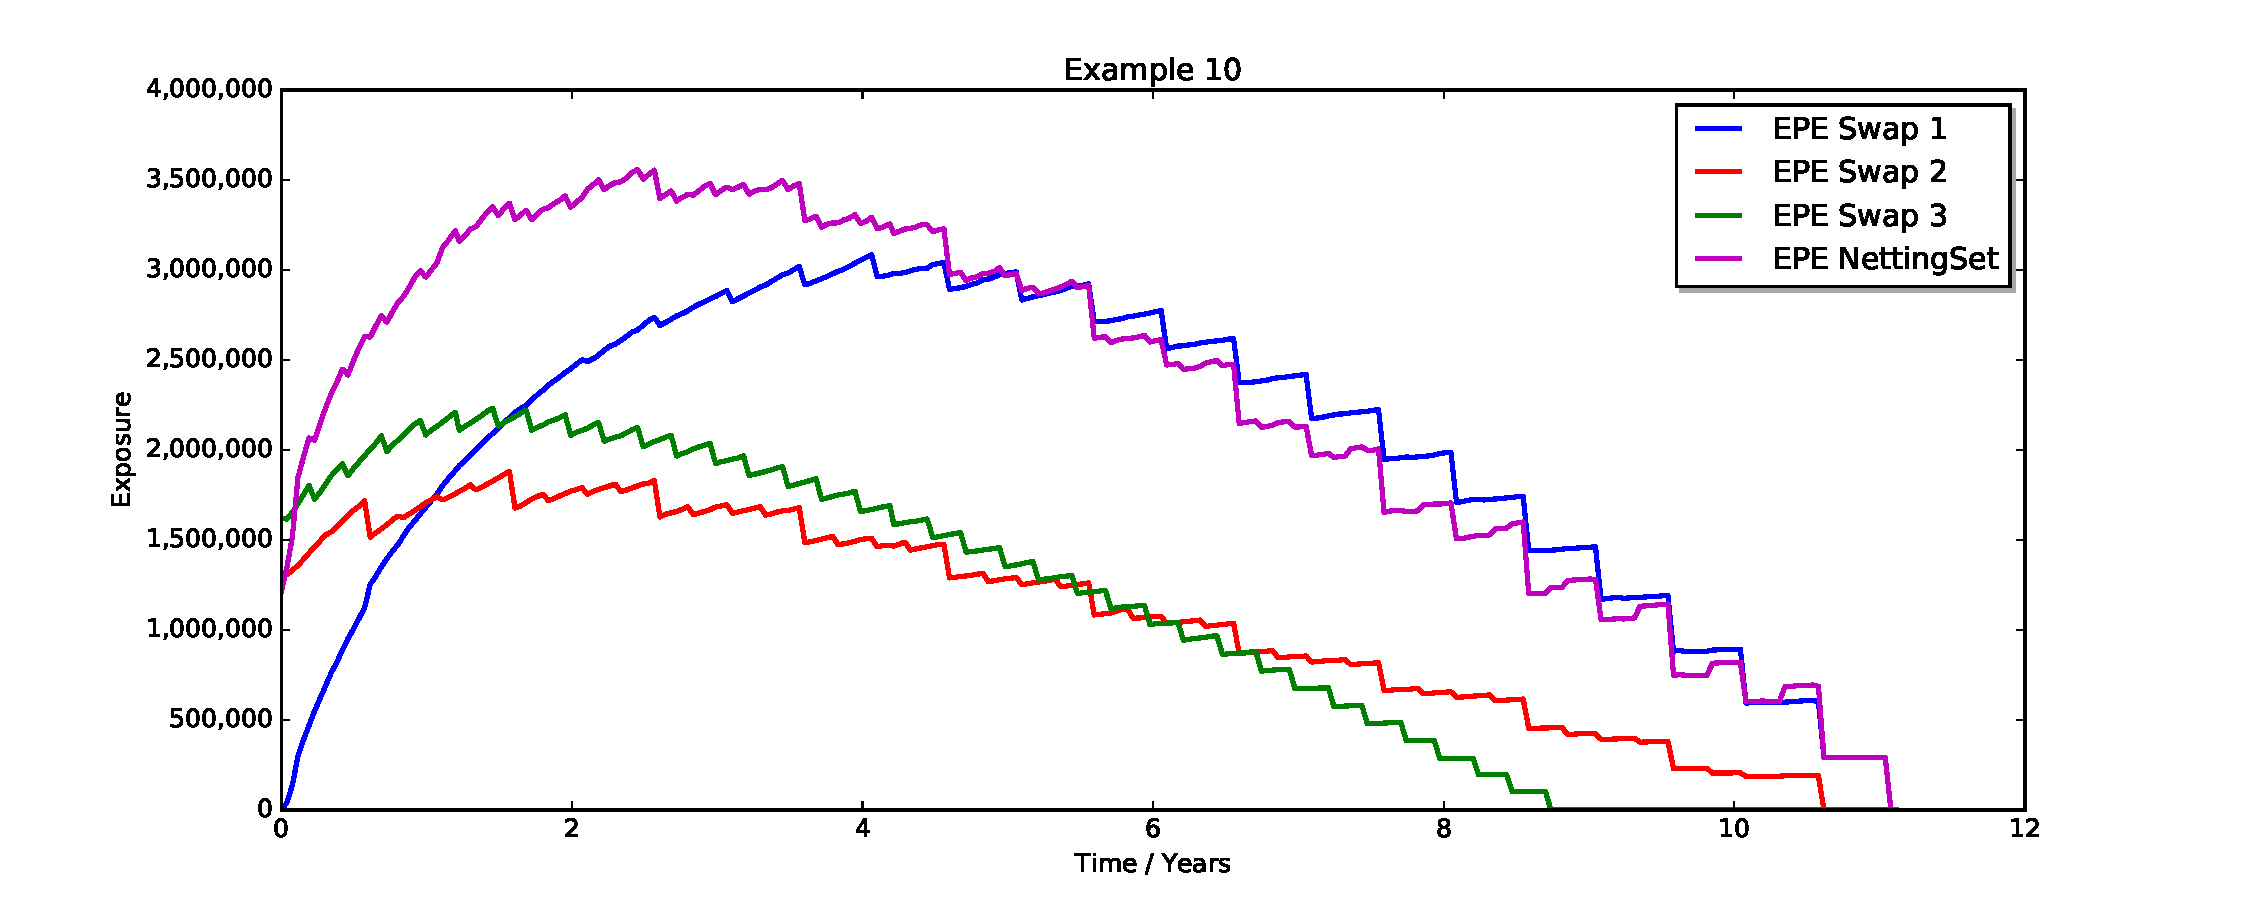
\includegraphics[scale=0.45]{mpl_nocollateral_epe.pdf}
\end{center}
\caption{Three swaps netting set, no collateral. Simulation with 5000 paths and bi-weekly time steps.}
\label{fig_8}
\end{figure}

\begin{figure}[htb]
\begin{center}
%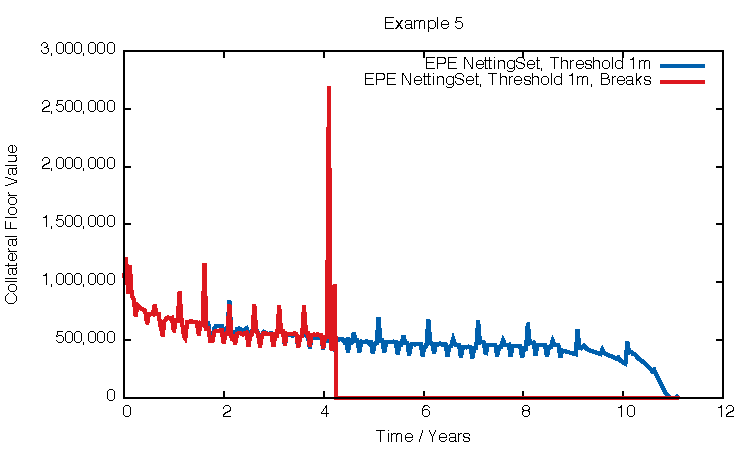
\includegraphics[scale=1.0]{example_threshold_break_epe.pdf}
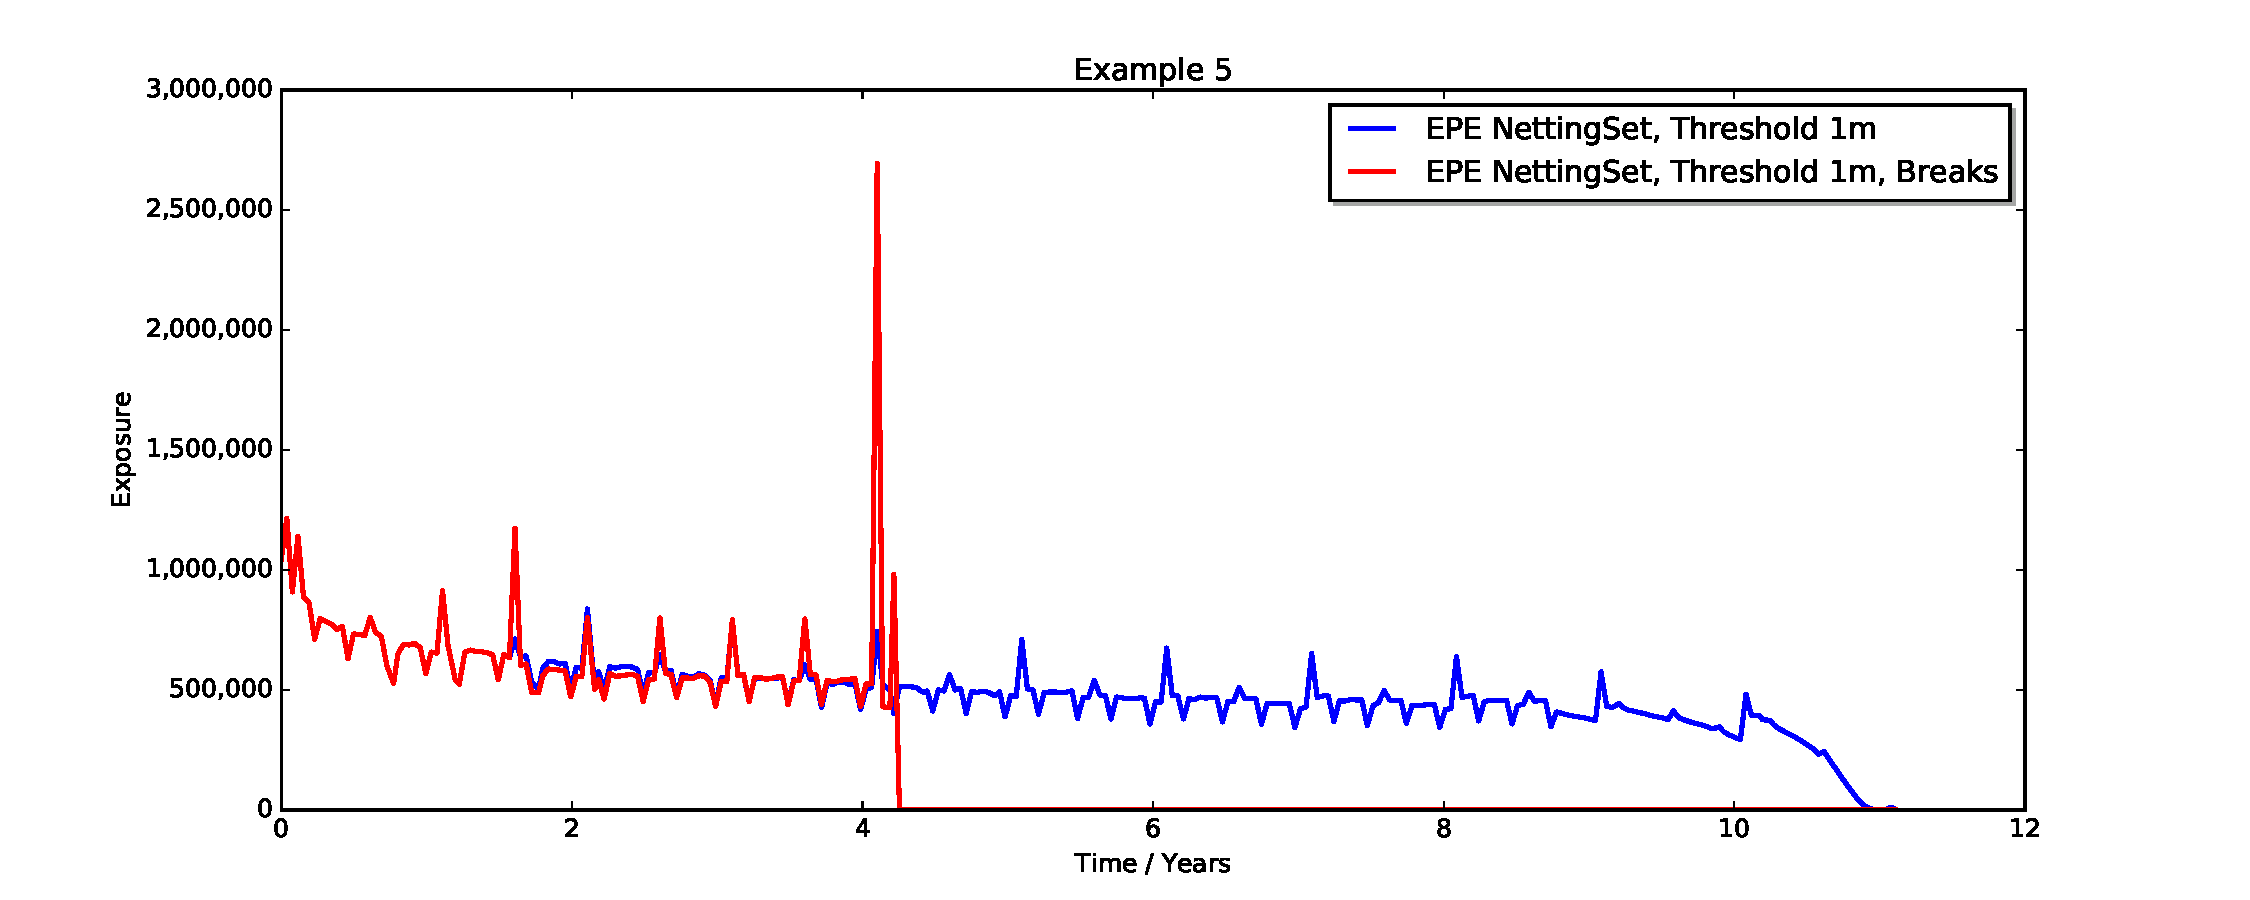
\includegraphics[scale=0.45]{mpl_threshold_break_epe.pdf}
\end{center}
\caption{Three swaps netting set, THR=1m EUR, MTA=100k EUR, MPoR=2w. The red evolution assumes that the each trade is terminated at the next break date. The blue evolution ignores break dates. Simulation with 5000 paths and bi-weekly time steps.}
\label{fig_9}
\end{figure}

%\begin{figure}[hbt]
%\begin{center}
%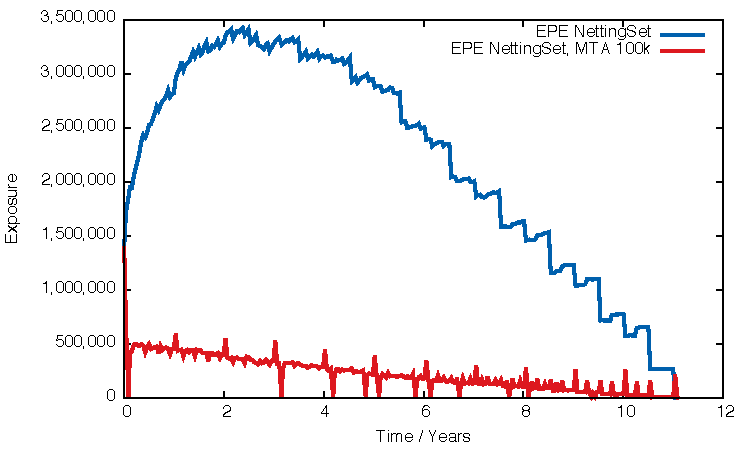
\includegraphics[scale=1.0]{example_mta_epe.pdf}
%\end{center}
%\caption{Three swaps, threshold = 0, mta > 0.}
%\label{fig_7}
%\end{figure}

\begin{figure}[htb]
\begin{center}
%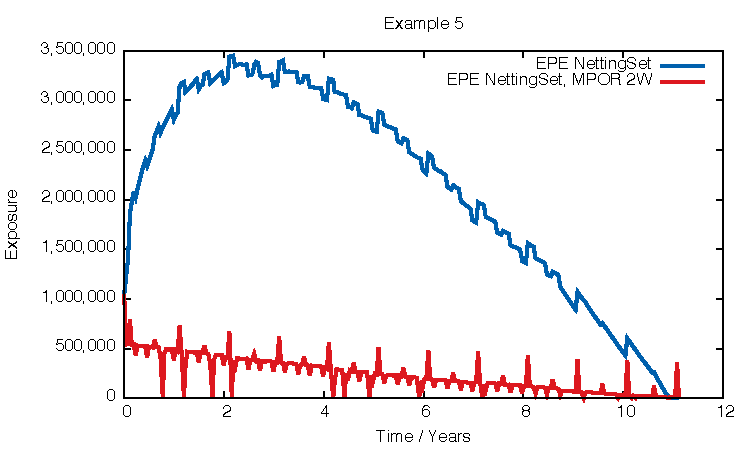
\includegraphics[scale=1.0]{example_mpor_epe.pdf}
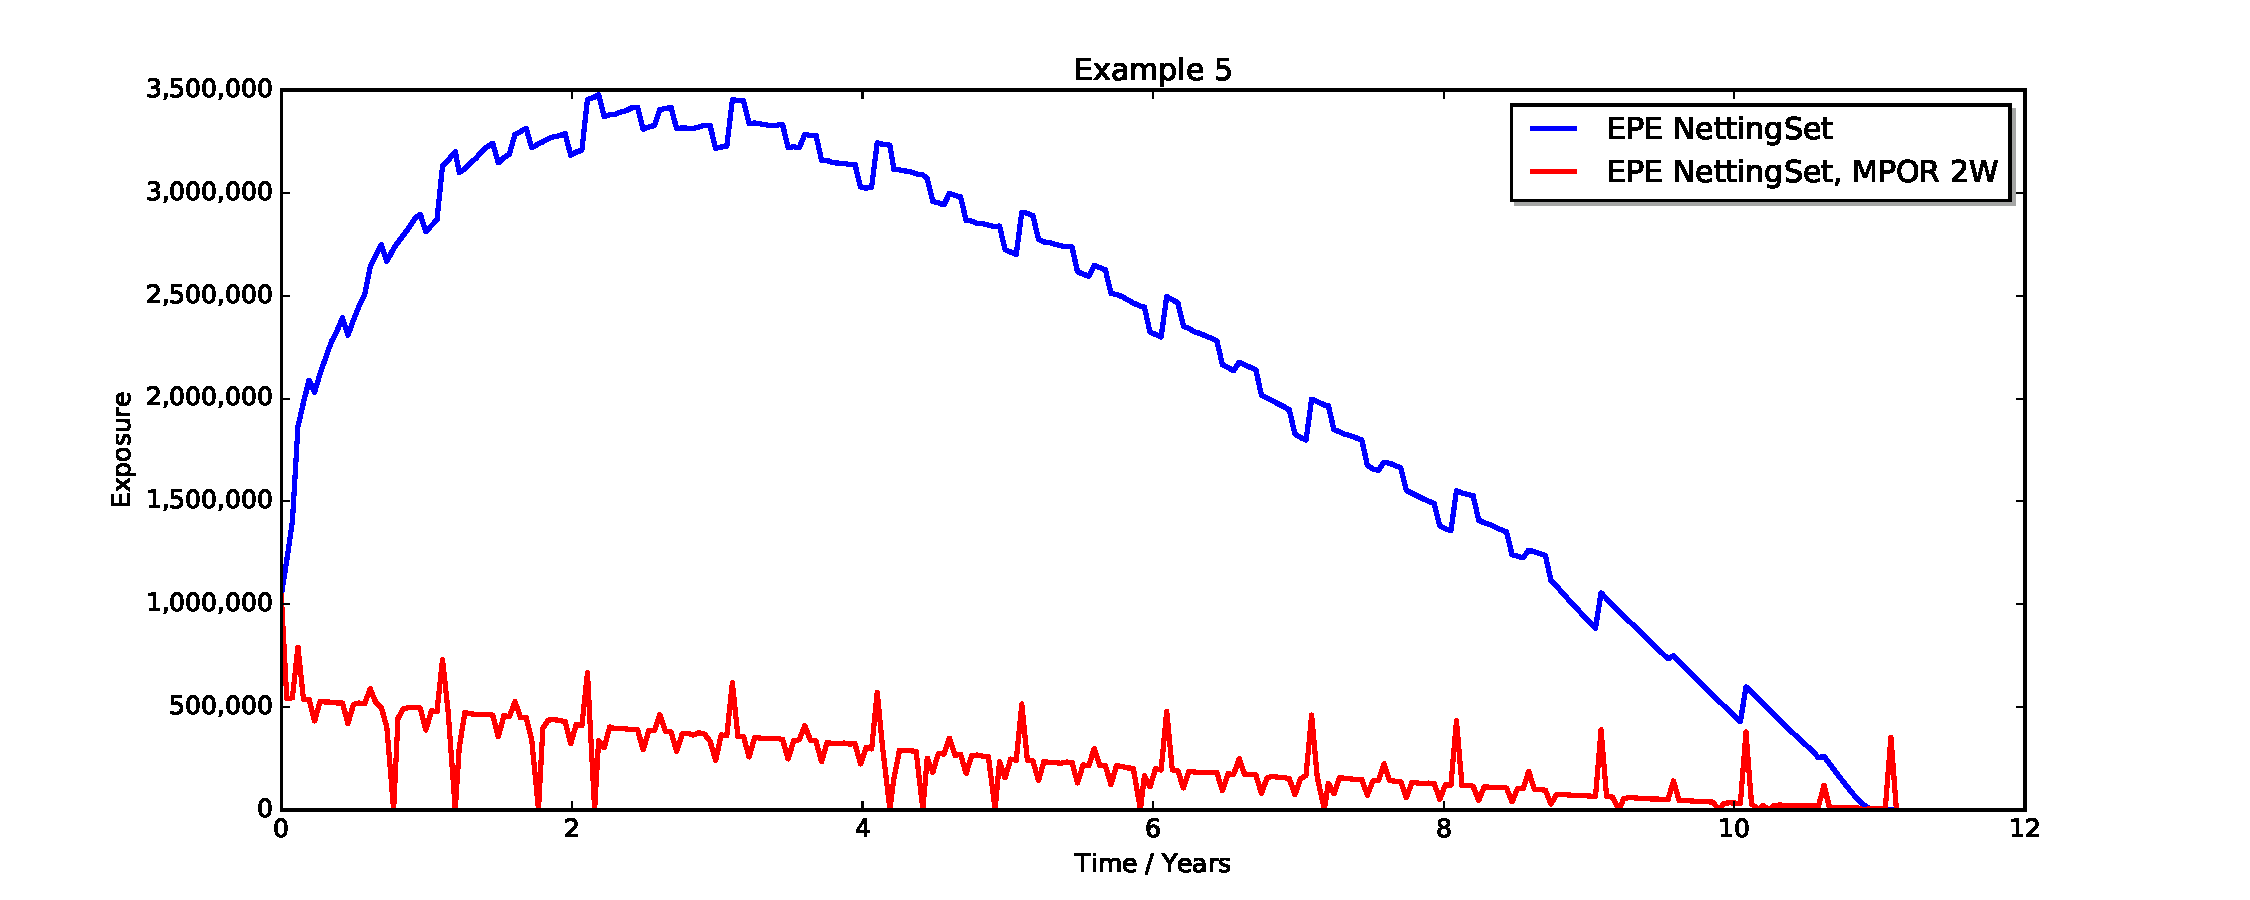
\includegraphics[scale=0.45]{mpl_mpor_epe.pdf}
\end{center}
\caption{Three swaps, THR=MTA=0, MPoR=2w. Simulation with 5000 paths and bi-weekly time steps.}
\label{fig_10}
\end{figure}

%--------------------------------------------------------
\subsection{CVA, DVA, FVA, COLVA and Collateral Floor}
%--------------------------------------------------------

We use one of the cases in {\tt Examples/Example\_5} to demonstrate the
XVA outputs, see folder {\tt Examples/Example\_5/Output/collateral\_threshold}.

\medskip
The summary of CVA, DVA, FVA, COLVA and Collateral Floor is provided in file {\tt xva.csv}. 
The file includes the allocated CVA and DVA numbers to individual trades as introduced in the next section. The following table illustrates the file's layout,
omitting the three right-most columns containing allocated data. 

\begin{center}
\footnotesize
\begin{tabular}{|l|l|r|r|r|r|r|r|}
\hline
TradeId & NettingSetId & CVA & DVA & FBA & FCA & COLVA & CollateralFloor \\ %& AllocatedCVA & AllocatedDVA & AllocationMethod \\
\hline
	& CPTY\_A & 31,084 	& 45,003 &	-4,803 &	 21,233 & 	 2,089 &	 182,351 \\
Swap\_1 & CPTY\_A &	 115,944 &	 210,630 &	-17,864 &	 99,984 &	 n/a &	 n/a \\
Swap\_2 & CPTY\_A &	 67,683 &	 96,412 &	-10,588 &	 45,488 &	 n/a &	 n/a \\
Swap\_3 & CPTY\_A &	 71,299 & 	 84,752 & 	-11,268 & 	 40,327 & 	 n/a &	 n/a \\
\hline
\end{tabular}
\end{center}

The line(s) with empty TradeId column contain values at netting set level, the others contain uncollateralised single-trade VAs.
Note that COLVA and Collateral Floor are only available at netting set level at which collateral is posted.

\medskip
Detailed output is written for COLVA and Collateral Floor to file {\tt colva\_nettingset\_*.csv} which shows the 
incremental contributions to these two VAs through time.


%--------------------------------------------------------
\subsection{Exposure Reports \& XVA Allocation to Trades}
%--------------------------------------------------------

Using the example in folder {\tt Examples/Example\_5} we illustrate here the layout of an exposure report produced by ORE. The report shows the exposure evolution of Swap\_1 without collateral which - after running Example\_5 - is found in folder \\
{\tt Examples/Example\_5/Output/collateral\_none/exposure\_trade\_Swap\_1.csv}:

\begin{center}
\footnotesize
\begin{tabular}{|l|l|l|r|r|r|r|r|}
\hline
\#TradeId&Date& Time & EPE & ENE & AllocatedEPE & AllocatedENE & PFE \\
\hline
Swap\_1&05/02/16& 0.0000 & 0 & 1,711,850 & 0  & 0  & 0 \\
Swap\_1&19/02/16& 0.0383 & 40,177 & 1,744,040 &-1,190,880 & 512,983 & 263,485 \\
Swap\_1&04/03/16& 0.0765 & 137,451 & 1,840,660 &-915,192 & 788,016 & 1,053,240 \\
Swap\_1&18/03/16& 0.1148 & 298,993 & 1,742,290 &-651,132 & 792,160 & 1,913,310 \\
Swap\_1&01/04/16& 0.1530 & 389,983 & 1,834,620 &-552,148 & 892,485 & 2,372,650 \\
Swap\_1&15/04/16& 0.1913 & 471,627 & 1,918,380 &-466,365 & 980,387 & 2,764,670 \\
Swap\_1&29/04/16& 0.2295 & 550,054 & 2,000,390 &-331,155 & 1,119,180 & 3,105,720 \\
Swap\_1&13/05/16& 0.2678 & 620,006 & 2,074,610 &-266,147 & 1,188,450 & 3,425,930 \\
Swap\_1&27/05/16& 0.3060 & 689,726 & 2,140,030 &-191,144 & 1,259,160 & 3,777,310 \\
Swap\_1&10/06/16& 0.3443 & 762,894 & 2,205,710 &-137,876 & 1,304,940 & 4,051,510 \\
Swap\_1 & ... & ...& ... & ... & ... & ... & ... \\
\hline
\end{tabular}
\end{center}

The exposure measures EPE, ENE and PFE are defined in appendix \ref{sec:app_exposure}. Allocated exposures are defined in appendix \ref{sec:app_allocation}. The PFE quantile and allocation method are chosen as described in section \ref{sec:analytics}.

In addition to single trade exposure files, ORE produces an exposure file per netting set. The example from the same folder as above is:

\begin{center}
\footnotesize
\begin{tabular}{|l|l|l|r|r|r|r|r|}
\hline
\#NettingSet&Date& Time & EPE & ENE & PFE & ExpectedCollateral \\ 
\hline
%CPTY\_A&05/02/16& 0.0000 & 1,211,770 & 0  & 1,211,770 &-1,211,770 \\
CPTY\_A&05/02/16& 0.0000 & 1,211,770 & 0  & 1,211,770 & 0 \\
CPTY\_A&19/02/16& 0.0383 & 1,344,230 & 137,779 & 3,414,420 & 0   \\
CPTY\_A&04/03/16& 0.0765 & 1,518,610 & 308,388 & 4,353,770 & 0   \\
CPTY\_A&18/03/16& 0.1148 & 1,846,910 & 382,078 & 5,201,760 & 0   \\
CPTY\_A&01/04/16& 0.1530 & 1,961,310 & 494,438 & 5,868,340 & 0   \\
CPTY\_A&15/04/16& 0.1913 & 2,067,270 & 598,315 & 6,385,360 & 0   \\
CPTY\_A&29/04/16& 0.2295 & 2,053,700 & 745,986 & 6,738,990 & 0   \\
CPTY\_A&13/05/16& 0.2678 & 2,149,220 & 845,534 & 6,926,730 & 0   \\
CPTY\_A&27/05/16& 0.3060 & 2,235,660 & 930,251 & 7,293,950 & 0   \\
CPTY\_A&10/06/16& 0.3443 & 2,314,510 & 1,014,740 & 7,752,770 & 0   \\
CPTY\_A & ... & ...& ... & ... & ... & ... \\
\hline
\end{tabular}
\end{center}

Allocated exposures are missing here, as they make sense at the trade level only, and the expected collateral balance is added for information (in this case zero as collateralisation is deactivated in this example).

\medskip
{\tt Examples/Example\_5} features the allocation of netting set exposure and XVA to the trade level as frequently required by finance departments. We start again with the uncollateralised case in figure \ref{fig_8}, followed by the case with threshold 1m EUR in figure \ref{fig_9}.
\begin{figure}[tb]
\begin{center}
%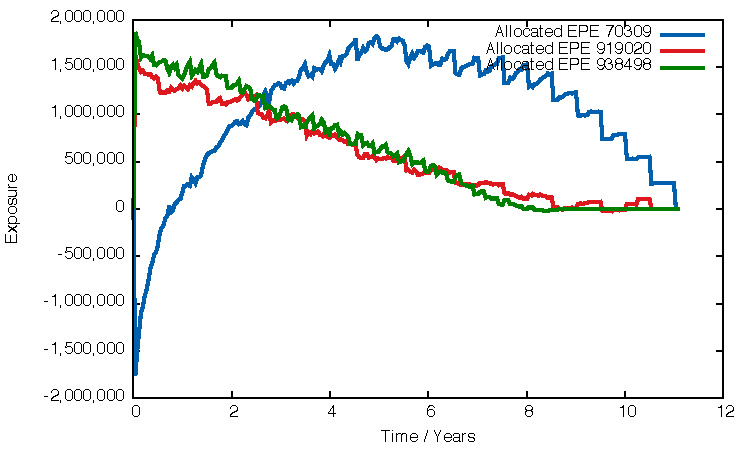
\includegraphics[scale=1.0]{example_nocollateral_allocated_epe.pdf}
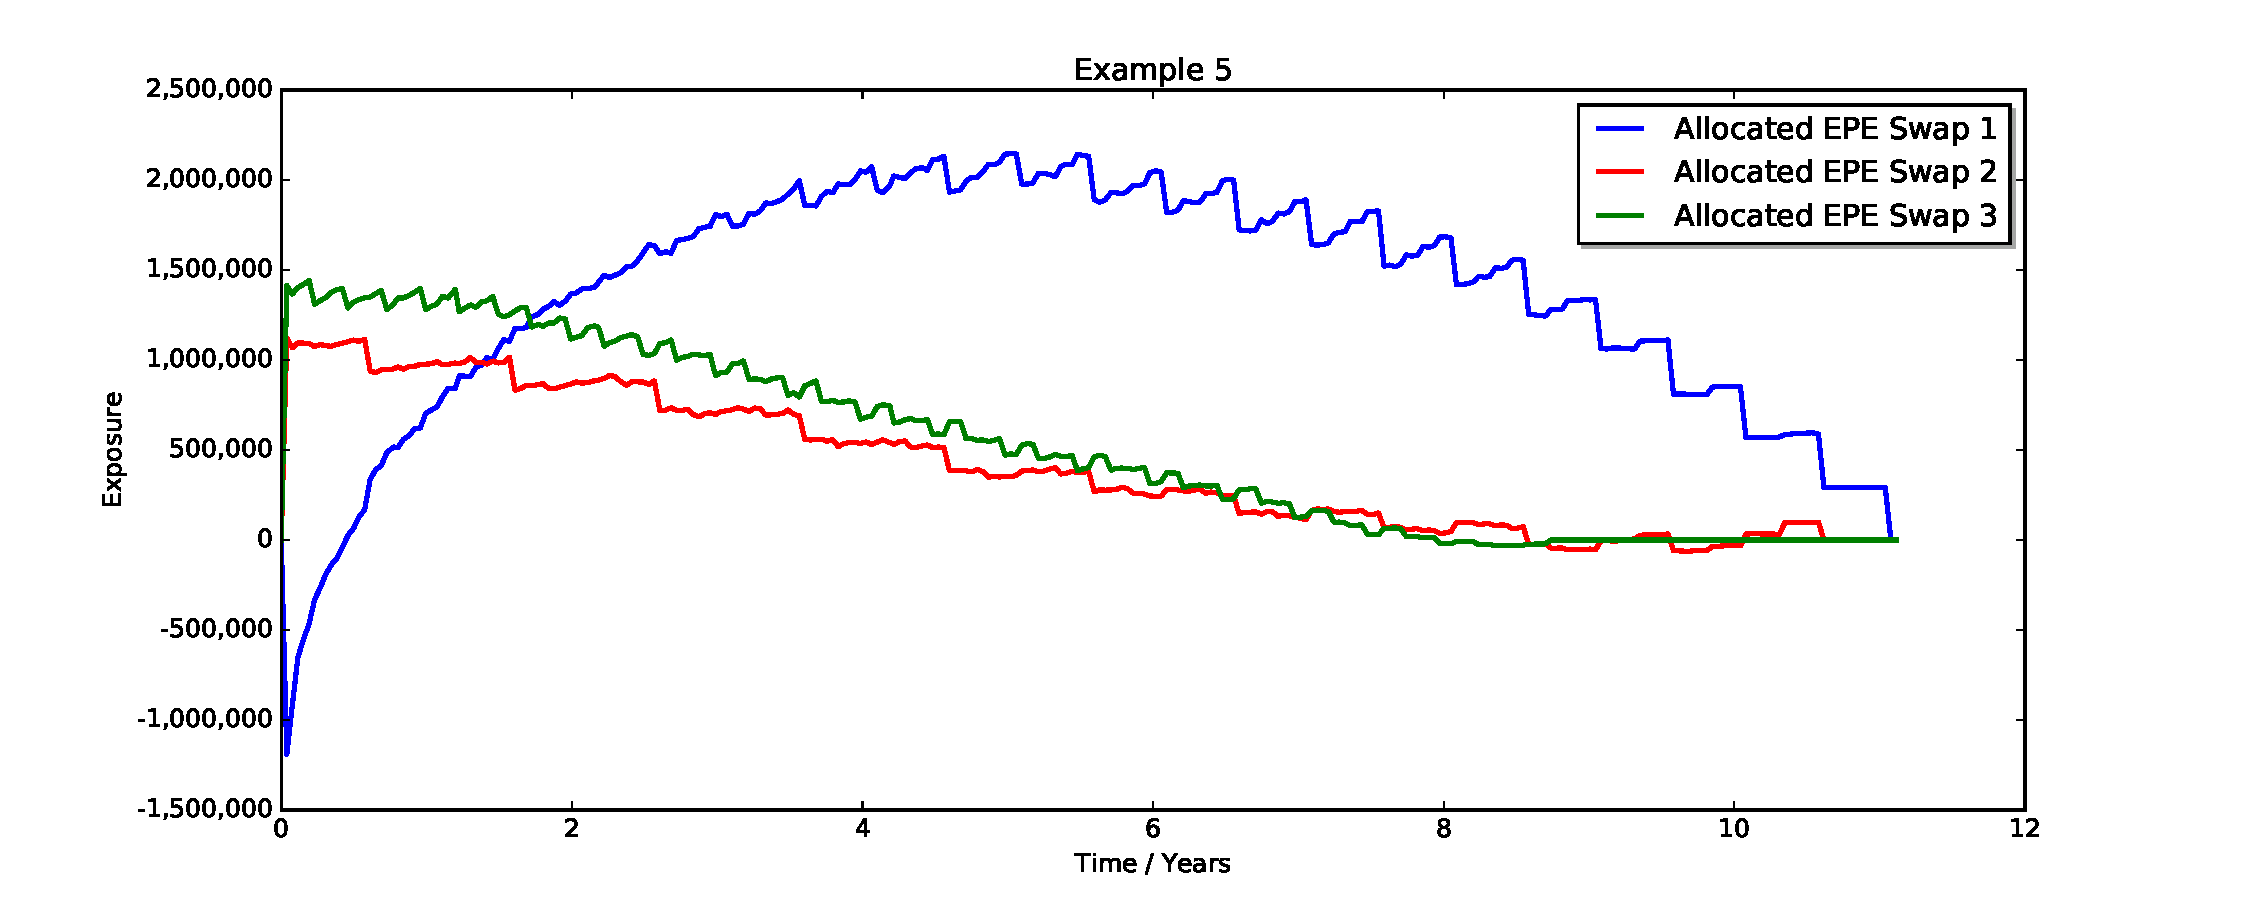
\includegraphics[scale=0.45]{mpl_nocollateral_allocated_epe.pdf}
\end{center}
\caption{Exposure allocation without collateral. Simulation with 5000 paths and bi-weekly time steps.}
\label{fig_12}
\end{figure}
In both cases we apply the {\em marginal} (Euler) allocation method as published by Pykhtin and Rosen in 2010, hence we see the typical negative EPE for one of the trades at times when it reduces the netting set exposure. The case with collateral moreover shows the typical spikes in the allocated exposures.
\begin{figure}[tb]
\begin{center}
%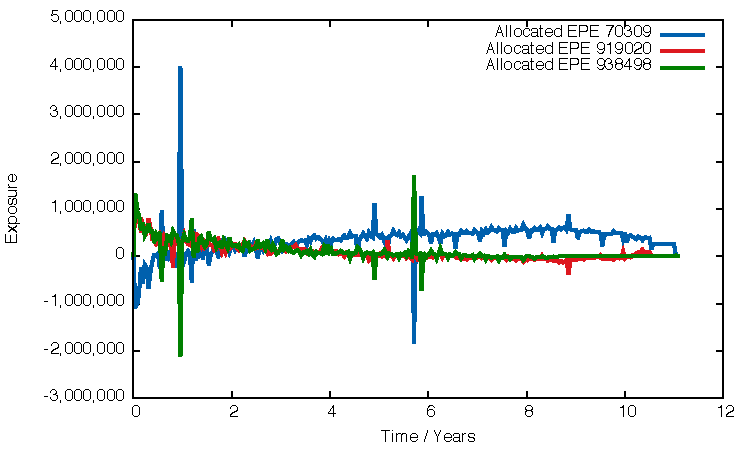
\includegraphics[scale=1.0]{example_threshold_allocated_epe.pdf}
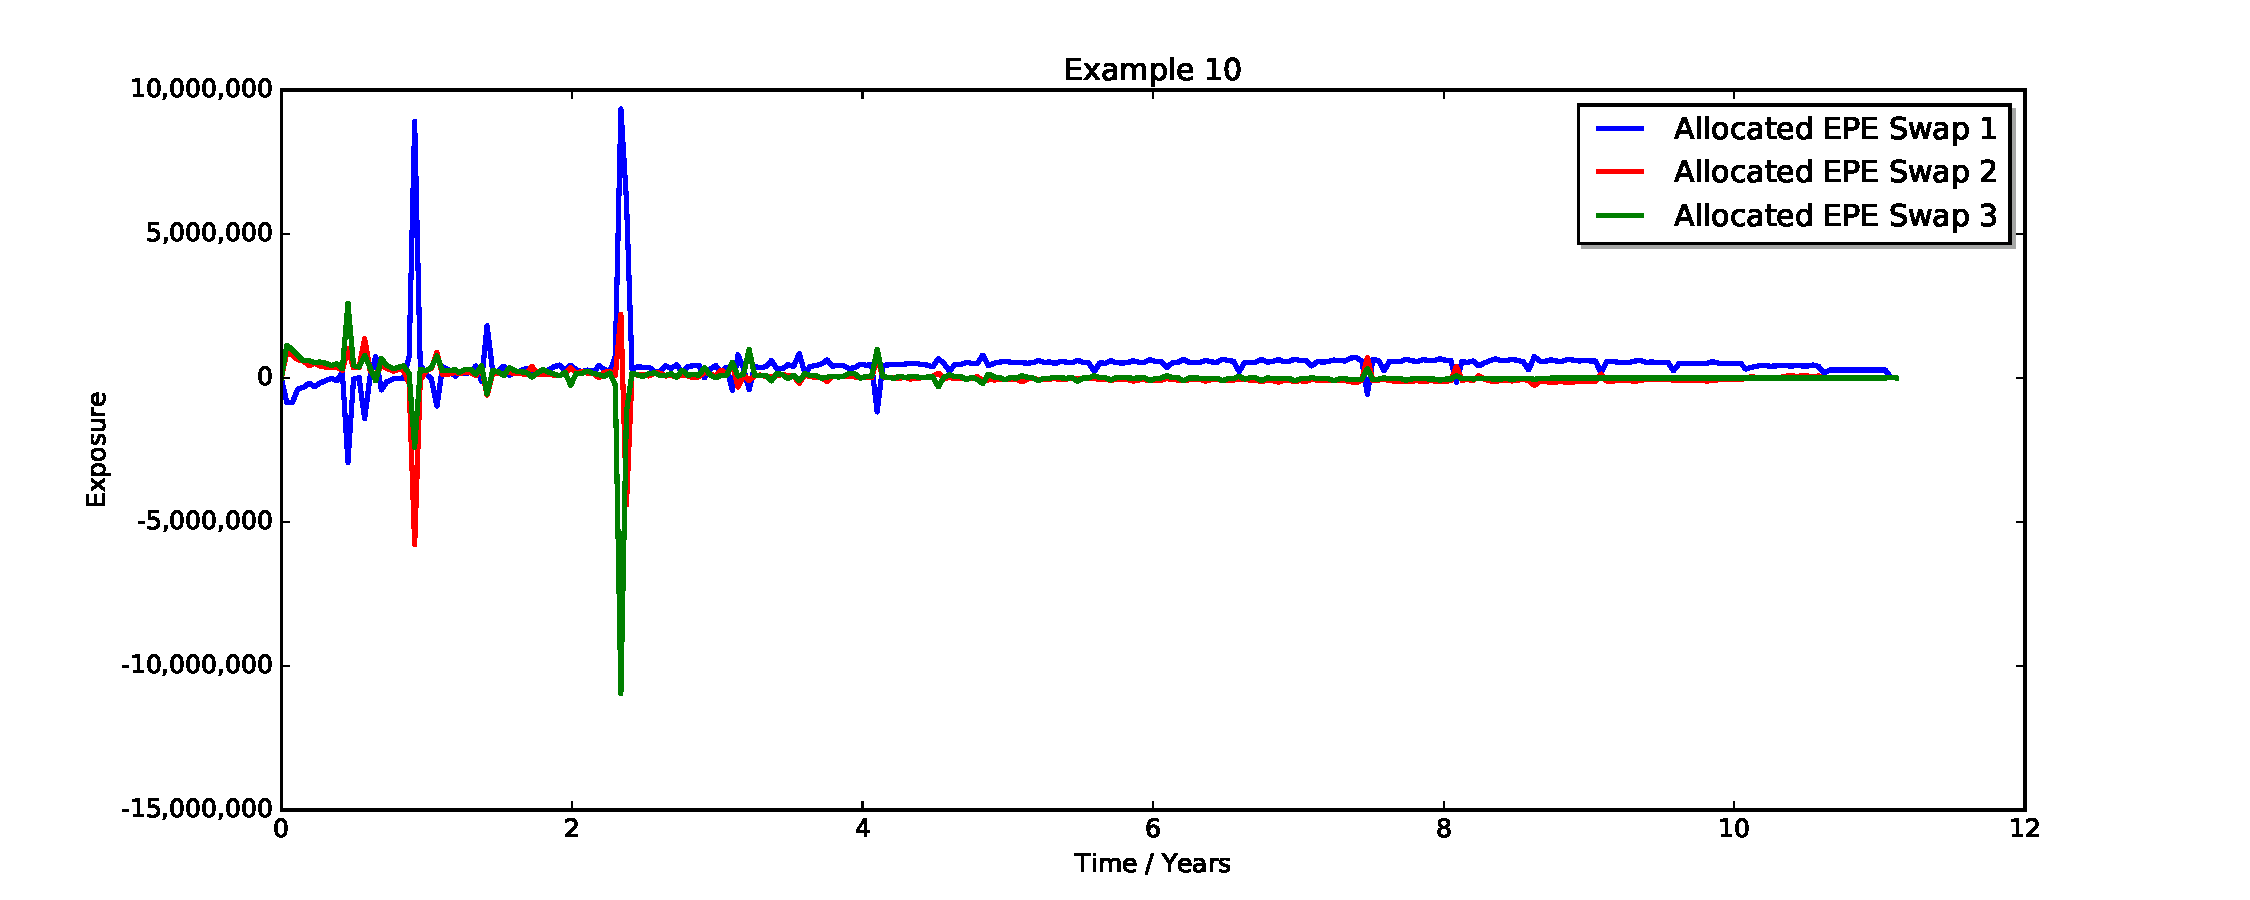
\includegraphics[scale=0.45]{mpl_threshold_allocated_epe.pdf}
\end{center}
\caption{Exposure allocation with collateral and threshold 1m EUR. Simulation with 5000 paths and bi-weekly time steps.}
\label{fig_13}
\end{figure}
The analytics results also feature allocated XVAs in file {\tt xva.csv} which are derived from the allocated exposure profiles. Note that ORE also offers alternative allocation methods to the marginal method by Pykhtin/Rosen, which can be explored with {\tt Examples/Example\_5}.

\clearpage
%========================================================
\section{Launchers}\label{sec:visualisation}
%========================================================

\subsection{Jupyter}\label{sec:jupyter}

In this section we are going to show how to use Jypyter notebooks to 
\begin{itemize}
\item run the examples listed in the previous section, 
\item further analyse the NPV cube data
\end{itemize}

\todo[inline]{Add Jupyter section}

\subsection{Calc}\label{sec:calc}

ORE comes with a simple LibreOffice Calc \cite{LO} sheet as an ORE launcher and basic result viewer. This is demonstrated on the example in section \ref{sec:example1}. It is currently based on the stable LibreOffice version 5.0.6 and tested on OS X. 

To launch Calc, open a terminal, change to directory {\tt Examples/Example\_1}, and run

\medskip
{\centerline{\tt ./launchCalc.sh} }
\medskip

%This will show the blank sheet in figure \ref{fig_14}.
%\begin{figure}[hbt]
%\begin{center}
%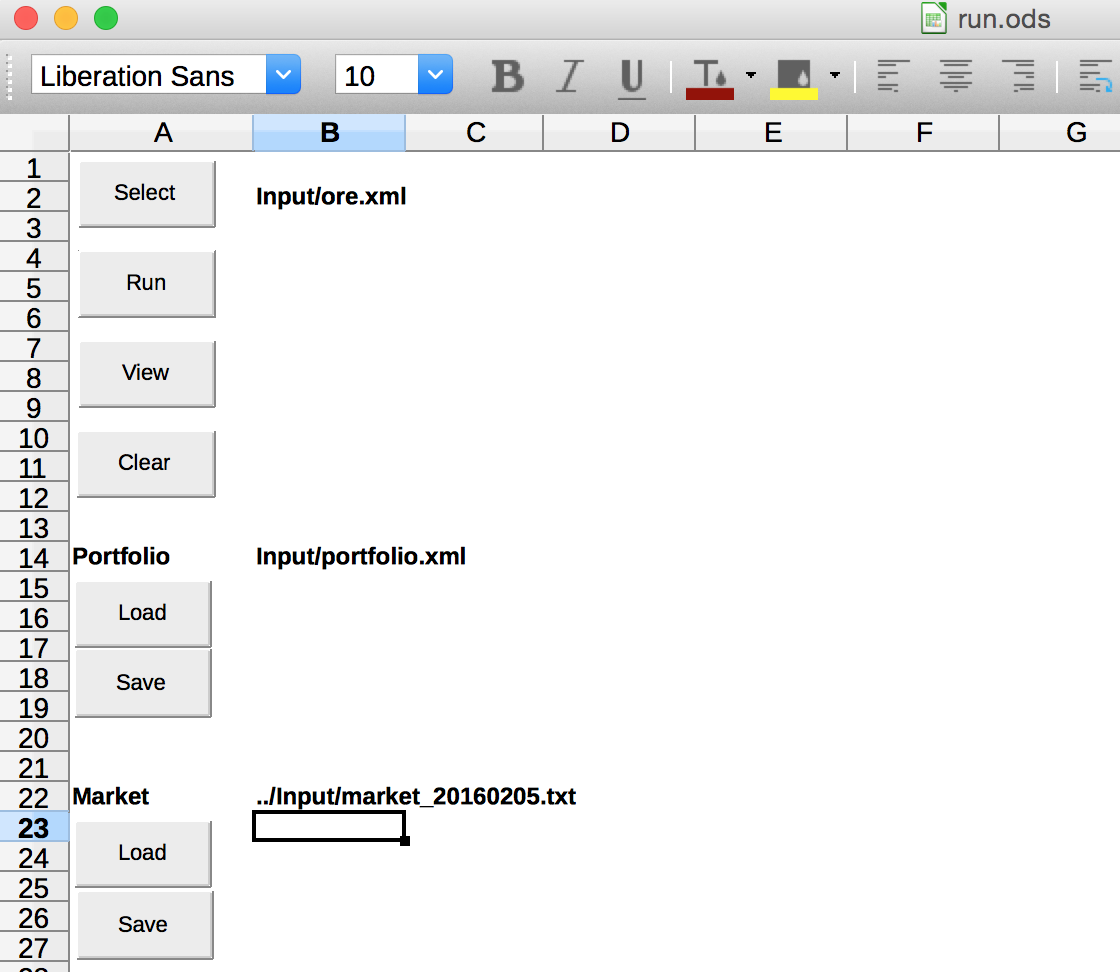
\includegraphics[scale=0.4]{demo_calc_1}
%\end{center}
%\caption{Calc sheet after launching.}
%\label{fig_14}
%\end{figure}
The user can choose a configuration (one of the {\tt ore*.xml} files in Example\_1's subfolder Input) by hitting the 'Select' button. Initially Input/ore.xml is pre-selected. The ORE process is then kicked off by hitting 'Run'. Once completed, standard ORE reports (NPV, Cashflow, XVA) are loaded into several sheets. Moreover, exposure evolutions can then be viewed by hitting 'View' which shows the result in figure \ref{fig_15}.  
\begin{figure}[hbt]
\begin{center}
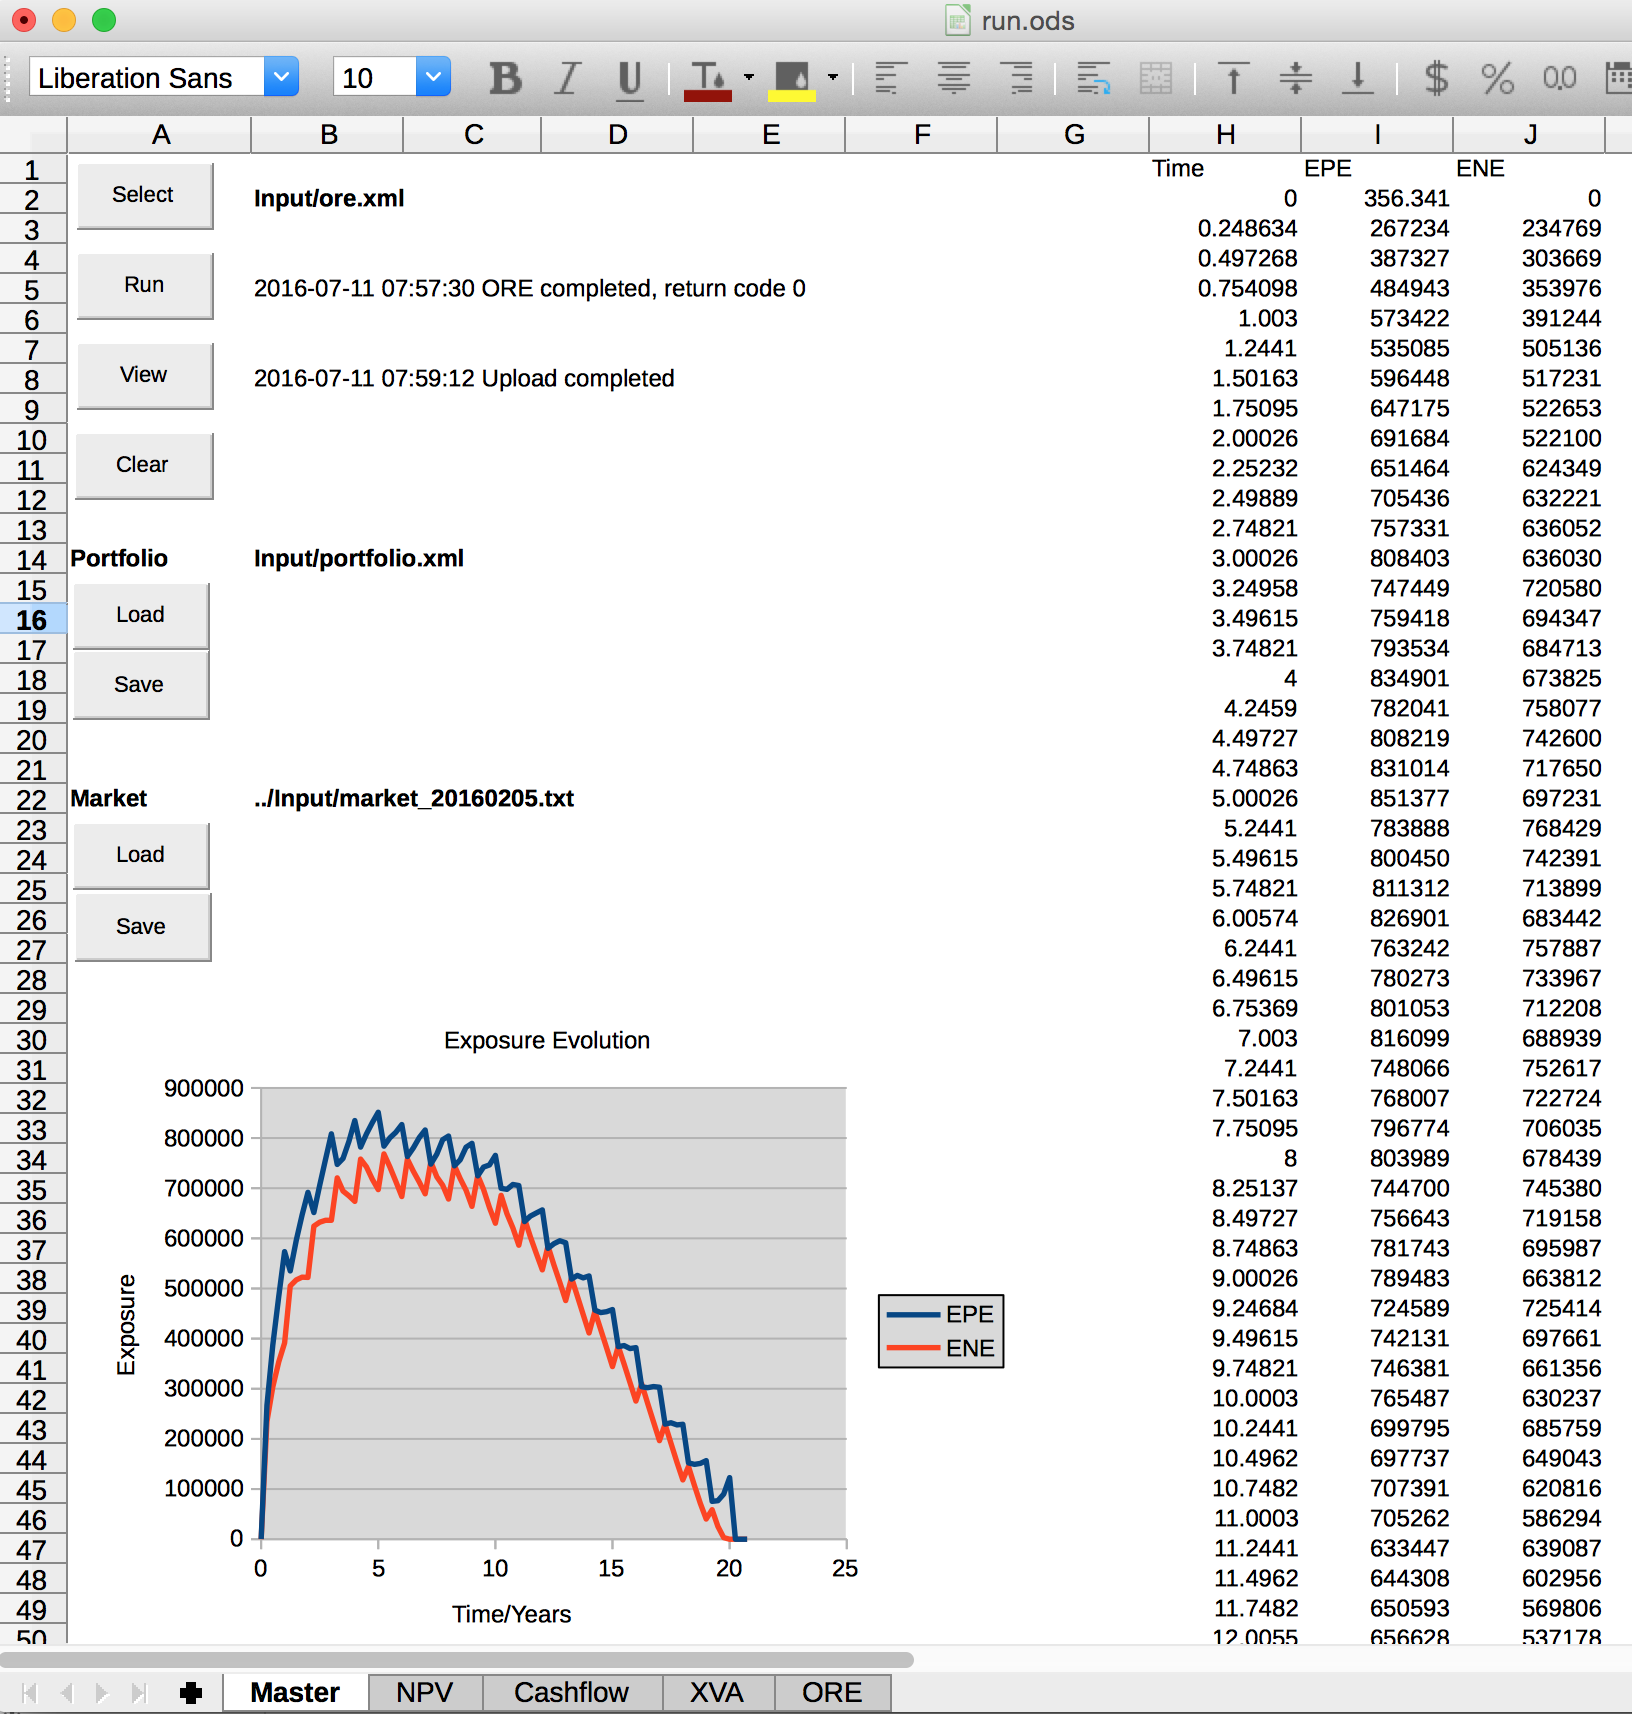
\includegraphics[scale=0.4]{demo_calc_2}
\end{center}
\caption{Calc sheet after hitting 'Run'.}
\label{fig_15}
\end{figure}

This demo uses simple Libre Office Basic macros which call Python scripts to execute ORE. The Libre Office Python uno module (which comes with Libre Office) is used to communicate between Python and Calc to upload results into the sheets. 

\todo[inline]{Remove hard-coded file names from Python scripts}
\todo[inline]{Calc example on Windows and Linux} 
%\todo[inline]{Support both OpenOffice and LibreOffice Calc.}
\todo[inline]{Harmonise layout with Excel launcher} 

\subsection{Excel}

For Microsoft Excel, similar interaction between Python and the spread sheet can be achieved with the  Python module {\tt xlwings} \cite{xlwings} on both Windows and Mac OSX.
However, unlike Libre Office where the uno Python module is part of the distribution, xlwings needs to be installed separately. We therefore rather demonstrate an Excel sheet here which uses VBA only to call the ORE application and load resulting data into the spreadsheet. This demo is available in Example\_1. Launch {\tt Example\_1.xlsm}. After launching the sheet, modify the paths on the first sheet, and then run the ORE process.

%========================================================
\section{Parametrisation}\label{sec:configuration}
%========================================================

ORE's batch version is kicked off with a single command line parameter 

\medskip
\centerline{\tt ore[.exe] ore.xml}
\medskip

which points to the 'master input file' referred to  as {\tt ore.xml} subsequently. 
This file is the starting point of the engine's configuration explained in the following sub section.

\subsection{Master Input File: {\tt ore.xml}}\label{sec:master_input}

The master input file contains general setup information (paths to configuration, trade data and market data), as well as the selection and configuration of  analytics to produce. The file has an opening and closing root element {\tt <OpenRiskEngine>}, {\tt </OpenRiskEngine>}, and within these three sections 
\begin{itemize}
\item Setup
\item Markets
\item Analytics
\end{itemize}
which we will explain in the following.

\subsubsection{Setup}

This subset of data is easiest explained using an example, see listing \ref{lst:ore_setup}.
\begin{listing}[H]
%\hrule\medskip
\begin{minted}[fontsize=\footnotesize]{xml}
<Setup>
  <Parameter name="asofDate">2016-02-05</Parameter>
  <Parameter name="inputPath">Input</Parameter>
  <Parameter name="outputPath">Output</Parameter>
  <Parameter name="logFile">log.txt</Parameter>
  <Parameter name="marketDataFile">../../Input/market_20160205.txt</Parameter>
  <Parameter name="fixingDataFile">../../Input/fixings_20160205.txt</Parameter>
  <Parameter name="implyTodaysFixings">Y</Parameter>
  <Parameter name="curveConfigFile">../../Input/curveconfig.xml</Parameter>
  <Parameter name="conventionsFile">../../Input/conventions.xml</Parameter>
  <Parameter name="marketConfigFile">../../Input/todaysmarket.xml</Parameter>
  <Parameter name="pricingEnginesFile">../../Input/pricingengine.xml</Parameter>
  <Parameter name="portfolioFile">portfolio.xml</Parameter>
  <!-- None, Unregister, Defer or Disable -->
  <Parameter name="observationModel">Disable</Parameter>
</Setup>
\end{minted}
%\hrule
\caption{ORE setup example}
\label{lst:ore_setup}
\end{listing}

Parameter names are self explanatory: Input and output path are interpreted relative from the directory where the ORE script is started, but can also be specified using absolute paths. All file names are then interpreted relative to the 'inputPath' and 'outputPath', respectively. The files starting with {\tt ../../Input/} then point to files in the global Example input directory {\tt Example/Input/*}, whereas files such as {\tt portfolio.xml} are local inputs in {\tt Example/Example\_\#/Input/}.

When ORE starts, it will initialise today's market, i.e. load market data and fixings, and build all term structures as specified in {\tt todaysmarket.xml}. 
Moreover, ORE will load the trades in {\tt portfolio.xml} and link them with pricing engines as specified in {\tt pricingengine.xml}. When parameter {\tt    
implyTodaysFixings} is set to Y, today's fixings would not be loaded but implied, relevant when pricing/bootstrapping off hypothetical market data as e.g. in scenario analysis and stress testing.

\medskip
The last parameter {\tt observationModel} can be used to control ORE performance during simulation. The choices {\em Disable }�and {\em Unregister } yield similarly improved performance relative to choice {\em None}. For users familiar with the QuantLib design - the parameter controls to which extent {\em QuantLib observer notifications} are used when market and fixing data is updated and the evaluation date is shifted: 
\begin{itemize}
\item The 'Unregister' option limits the amount of notifications by unregistering floating rate coupons from indices;
\item Option 'Defer' disables all notifications during market data and fixing updates with
{\tt ObservableSettings::instance().disableUpdates(true)}
and kicks off updates afterwards when enabled again
\item The 'Disable' option goes one step further and disables all notifications during market data and fixing updates, and in particular when the evaluation date is changed along a path, with \\
{\tt ObservableSettings::instance().disableUpdates(false)} \\
Updates are not deferred here. Required term structure and instrument recalculations are triggered explicitly. 
\end{itemize}
\todo[inline]{Expand the technical description of observationModel}

\subsubsection{Markets}\label{sec:master_input_markets}

The {\tt Markets} section (see listing \ref{lst:ore_markets}) is used to choose the two market configurations for simulation model calibration and the subsequent market simulation phase, respectively. These configurations have to be defined in {\tt todaysmarket.xml} (see section \ref{sec:market}). 

\begin{listing}[H]
%\hrule\medskip
\begin{minted}[fontsize=\footnotesize]{xml}
<Markets>
  <Parameter name="lgmcalibration">collateral_inccy</Parameter>
  <Parameter name="fxcalibration">collateral_eur</Parameter>
  <Parameter name="pricing">collateral_eur</Parameter>
  <Parameter name="simulation">collateral_eur</Parameter>
</Markets>
\end{minted}
%\hrule
\caption{ORE markets}
\label{lst:ore_markets}
\end{listing}

For example, the calibration of the simulation model's interest rate components requires local OIS discounting whereas the simulation phase requires cross currency adjusted discount curves to get FX product pricing right. So far, the market configurations are used only to distinguish discount curve sets, but the market configuration concept in ORE applies to all term structure types.

\subsubsection{Analytics}\label{sec:analytics}

The {\tt Analytics} section lists all permissible analytics using tags {\tt <Analytic type="..."> ... </Analytic>} where type can be (so far) in
\begin{itemize}
\item npv
\item cashflow
\item curves
\item simulation
\item xva
\item initialMargin
\end{itemize}

Each {\tt Analytic} section contains a list of key/value pairs to parameterise the analysis of the form {\tt <Parameter name="key">value</Parameter>}. Each analysis
must have one key {\tt active} set to Y or N to activate/deactivate this analysis. 
The following listing \ref{lst:ore_analytics} shows the parametrisation of the first three basic analytics in the list above.

\begin{listing}[H]
%\hrule\medskip
\begin{minted}[fontsize=\footnotesize]{xml}
<Analytics>    
  <Analytic type="npv">
    <Parameter name="active">Y</Parameter>
    <Parameter name="baseCurrency">EUR</Parameter>
    <Parameter name="outputFileName">npv.csv</Parameter>
  </Analytic>      
  <Analytic type="cashflow">
    <Parameter name="active">Y</Parameter>
    <Parameter name="outputFileName">flows.csv</Parameter>
  </Analytic>      
  <Analytic type="curves">
    <Parameter name="active">Y</Parameter>
    <Parameter name="configuration">default</Parameter>
    <Parameter name="grid">240,1M</Parameter>
    <Parameter name="outputFileName">curves.csv</Parameter>
  </Analytic>
  <Analytic type="...">
    <!-- ... -->
  </Analytic>      
</Analytics>      
\end{minted}
\caption{ORE analytics: npv, cashflow and curves}
\label{lst:ore_analytics}
\end{listing}

The curves analytic exports all yield curves that have been built according to the specification in {\tt todaysmarket.xml}. Key {\tt configuration} selects the curve set to be used (see explanation in the previous Markets section).  Key {\tt grid} defines the time grid on which the yield curves are evaluated, in the example above a grid of 240 monthly time steps from today. The discount factors for all curves with configuration default will be exported on this monthly grid into the csv file specified by key {\tt outputFileName}. The grid can also be specified explicitly by a comma separated list of tenor points such as {\tt 1W, 1M, 2M, 3M, \dots}.

\medskip
The purpose of the {\tt simulation} 'analytics' is to run a Monte Carlo simulation which evolves the market as specified in the simulation config file. The primary result is an NPV cube file, i.e. valuations of all trades in the portfolio file (see section Setup), for all future points in time on the simulation grid and for all paths. Apart from the NPV cube, additional scenario data (such as simulated overnight rates etc) are stored in this process which are needed for subsequent XVA analytics.  

\begin{listing}[H]
%\hrule\medskip
\begin{minted}[fontsize=\footnotesize]{xml}
<Analytics>
  <Analytic type="simulation">
    <Parameter name="active">Y</Parameter>
    <Parameter name="simulationConfigFile">simulation.xml</Parameter>
    <Parameter name="pricingEnginesFile">../../Input/pricingengine.xml</Parameter>
    <Parameter name="baseCurrency">EUR</Parameter>
    <Parameter name="cubeFile">cube.dat</Parameter>
    <Parameter name="additionalScenarioDataFileName">scenariodata.dat</Parameter>
  </Analytic>
</Analytics>      
\end{minted}
\caption{ORE analytic: simulation}
\label{lst:ore_simulation}
\end{listing}

The pricing engines file specifies how trades are priced under future scenarios which can differ from pricing as of today (specified in section Setup).
Key base currency determines into which currency all NPVs will be converted. Key store scenarios (Y or N) determines whether the market scenarios are written to a file for later reuse.
\todo[inline]{Implement the store scenarios option, add file name to parametrisation}

\medskip
The xva analytic section offers CVA, DVA, FVA and COLVA calculations which can be selected/deselected here individually. All XVA calculations depend on a previously generated NPV cube (see above) which is referenced here via the {\tt cubeFile} parameter. This means one can re-run the xva analytics without regenerating the cube each time. The xva reports depend in particular on the settings in the {\tt csaFile} which determines CSA details such as margining frequency, collateral thresholds, minimum transfer amounts, margin period of risk. By splitting the processing into pre-processing (cube generation) and post-processing (aggregation and XVA analysis) it is possible to vary these CSA details and analyse their impact on XVAs quickly without re-generating the NPV cube.  

\begin{listing}[H]
%\hrule\medskip
\begin{minted}[fontsize=\footnotesize]{xml}
<Analytics>
  <Analytic type="xva">
    <Parameter name="active">Y</Parameter>
    <Parameter name="csaFile">netting.xml</Parameter>
    <Parameter name="cubeFile">cube.dat</Parameter>
    <Parameter name="scenarioFile">scenariodata.dat</Parameter>
    <Parameter name="baseCurrency">EUR</Parameter>
    <Parameter name="exposureProfiles">Y</Parameter>
    <Parameter name="quantile">0.95</Parameter>
    <Parameter name="calculationType">Symmetric</Parameter>      
    <Parameter name="allocationMethod">None</Parameter>    
    <Parameter name="marginalAllocationLimit">1.0</Parameter>
    <Parameter name="exerciseNextBreak">N</Parameter>
    <Parameter name="cva">Y</Parameter>
    <Parameter name="dva">N</Parameter>
    <Parameter name="dvaName">BANK</Parameter>
    <Parameter name="fva">N</Parameter>
    <Parameter name="fvaBorrowingCurve">BANK_EUR_BORROW</Parameter>
    <Parameter name="fvaLendingCurve">BANK_EUR_LEND</Parameter>
    <Parameter name="colva">Y</Parameter>
    <Parameter name="collateralSpread">0.0010</Parameter>
    <Parameter name="collateralFloor">Y</Parameter>
    <Parameter name="rawCubeOutputFile">rawcube.csv</Parameter>
    <Parameter name="netCubeOutputFile">netcube.csv</Parameter>     
  </Analytic>
</Analytics>
\end{minted}
\caption{ORE analytic: xva}
\label{lst:ore_xva}
\end{listing}

Parameters:
\begin{itemize}
\item {\tt csaFile:} Netting set definitions file covering CSA details such as margining frequency, thresholds, minimum transfer amounts, margin period of risk 
\item {\tt cubeFile:} NPV cube file previously generated and to be post-processed here
\item {\tt scenarioFile:} Scenario data previously generated and used in the post-processor (simulated index fixings and FX rates) 
\item {\tt baseCurrency:} Expression currency for all NPVs, value adjustments, exposures 
\item {\tt exposureProfiles:} Flag to enable/disable exposure output  
\item {\tt quantile} Confidence level for Potential Future Exposure (PFE) 
reporting
\item {\tt calculationType} Determines the settlement of margin calls: Symmetric - margin for both counterparties settled after the margin period of risk; AsymmetricCVA - margin requested from the counterparty settles with delay, margin requested from us settles immediately; AsymmetricDVA - vice versa). \todo[inline]{Move calculationType into the {\tt csaFile}?}   
\item {\tt allocationMethod:} XVA allocation method, choices are {\em None, Marginal, RelativeXVA} 
\item {\tt marginalAllocationLimit:} The marginal allocation method ala Pykhtin/Rosen breaks down when the netting set value vanishes while the exposure does not. This parameter acts as a cutoff for the marginal allocation when the absolute netting set value falls below this limit and switches to equal distribution of the exposure in this case.  
\item {\tt exerciseNextBreak:} Flag to terminate all trades at their next break date before aggregation and the subsequent analytics
\item {\tt cva, dva, fva, colva, collateralFloor:} Flags to enable/disable these analytics. \todo[inline]{Add collateral rates floor to the collateral model file (netting.xml)}
\item {\tt dvaName:} Credit name to look up the own default probability curve and recovery rate for DVA calculation
\item {\tt fvaBorrowingCurve:} Identifier of the borrowing yield curve 
\item {\tt fvaLendingCurve:} Identifier of the lending yield curve
\item {\tt collateralSpread:} Deviation between collateral rate and overnight rate, expressed in absolute terms (one basis point is 0.0001) assuming the day count convention of the collateral rate. \todo[inline]{Move collateralSpread to the collateral model file (netting.xml)}
\item {\tt rawCubeOutputFile:} File name for the trade NPV cube in human readable csv file format (per trade, date, sample)
\item {\tt netCubeOutputFile:} File name for the aggregated NPV cube in human readable csv file format (per netting set, date, sample) {\em after} taking collateral into account
\end{itemize}

The latter two cube file outputs are provided for interactive analysis and visualisation purposes, see section \ref{sec:visualisation}.

%--------------------------------------------------------
\subsection{Market: {\tt todaysmarket.xml}}\label{sec:market}
%--------------------------------------------------------

This configuration file determines the subset of the 'market' universe which is going to be built by ORE. It is the user's responsibility to make sure that this subset is sufficient to cover the portfolio to be analysed. If it is not, the application will complain at run time and exit.

\medskip
We assume that the market configuration is provided in file {\tt todaysmarket.xml}, however, the file name can be chosen by the user. The file name needs to be entered into the master configuration file {\tt ore.xml}, see section \ref{sec:master_input}.

\medskip
The file starts and ends with the opening and closing tags {\tt <TodaysMarket>} and {\tt </TodaysMarket>}. The file then contains configuration blocks for 
\begin{itemize}
\item Discounting curves
\item Index curves (to project index fixings)
\item Swap index curves (to project swap rates)
\item FX spot rates
\item FX Volatility structures
\item Swaption volatility structures
\item Cap/Floor volatility structures
\item Default curves
\end{itemize}

There can be alternative versions of each block each labeled with a unique identifier (e.g. Discount curve block with ID 'default', discount curve block with ID 'ois', another one with ID 'xois', etc). The purpose of these IDs will be explained at the end of this section. We now discuss each block's layout.

\subsubsection{Discounting Curves} 

We pick one discounting curve block as an example here (see {\tt Examples/Input/todaysmarket.xml}), the one with ID 'ois' 

\begin{listing}[H]
%\hrule\medskip
\begin{minted}[fontsize=\footnotesize]{xml}
  <DiscountingCurves Id="ois">
    <DiscountingCurve Currency="EUR">Yield/EUR/EUR1D</DiscountingCurve>
    <DiscountingCurve Currency="USD">Yield/USD/USD1D</DiscountingCurve>
    <DiscountingCurve Currency="GBP">Yield/GBP/GBP1D</DiscountingCurve>
    <DiscountingCurve Currency="CHF">Yield/CHF/CHF6M</DiscountingCurve>
    <DiscountingCurve Currency="JPY">Yield/JPY/JPY6M</DiscountingCurve>
    <!-- ... -->
  </DiscountingCurves>
\end{minted}
\caption{Discount curve block with ID 'ois'}
\label{lst:discountcurve_spec}
\end{listing}

This block instructs ORE to build five discount curves for the indicated currencies. The string within the tags, e.g. Yield/EUR/EUR1D, uniquely identifies the curve to be built.  Curve Yield/EUR/EUR1D is defined in the curve configuration file explained in section \ref{sec:curveconfig} below. In this case ORE is instructed to build an Eonia Swap curve made of Overnight Deposit and Eonia Swap quotes. The right most token of the string Yield/EUR/EUR1D (EUR1D) is user defined, the first two tokens Yield/EUR have to be used to point to a yield curve in currency EUR.
 
\subsubsection{Index Curves} 

See an excerpt of the index curve block with ID 'default' from the same example file:

\begin{listing}[H]
%\hrule\medskip
\begin{minted}[fontsize=\footnotesize]{xml}
<IndexForwardingCurves Id="default">
  <Index Name="EUR-EURIBOR-3M">Yield/EUR/EUR3M</Index>
  <Index Name="EUR-EURIBOR-6M">Yield/EUR/EUR6M</Index>
  <Index Name="EUR-EURIBOR-12M">Yield/EUR/EUR6M</Index>
  <Index Name="EUR-EONIA">Yield/EUR/EUR1D</Index>
  <Index Name="USD-LIBOR-3M">Yield/USD/USD3M</Index>
  <!-- ... -->
</IndexForwardingCurves>
\end{minted}
\caption{Index curve block with ID 'default'}
\label{lst:indexcurve_spec}
\end{listing}

This block of curve specifications instructs ORE to build another set of yield curves, unique strings (e.g. Yield/EUR/EUR6M etc.) point to the {\tt curveconfig.xml} file where these curves are defined. Each curve is then associated with an index name (of format Ccy-IndexName-Tenor, e.g. EUR-EURIBOR-6M) so that ORE will project the respective index using the selected curve (e.g. Yield/EUR/EUR6M).

\subsubsection{Swap Index Curves}

The following is an excerpt of the swap index curve block with ID 'default' from the same example file:

\begin{listing}[H]
%\hrule\medskip
\begin{minted}[fontsize=\footnotesize]{xml}
<SwapIndexCurves Id="default">
  <SwapIndex Name="EUR-CMS-1Y">
    <Index>EUR-EURIBOR-6M</Index>
    <Discounting>EUR-EONIA</Discounting>
  </SwapIndex>
  <SwapIndex Name="EUR-CMS-30Y">
    <Index>EUR-EURIBOR-6M</Index>
    <Discounting>EUR-EONIA</Discounting>
  </SwapIndex>
  <!-- ... -->
</SwapIndexCurves>
\end{minted}
\caption{Swap index curve block with ID 'default'}
\label{lst:swapindexcurve_spec}
\end{listing}

These instructions do not build any additional curves. They only build the respective swap index objects and associate them with the required index forwarding and discounting curves already built above. This enables a swap index to project the fair rate of forward starting Swaps. Swap indices are also containers for conventions. Swaption volatility surfaces require two swap indices each available in the market object, a long term and a short term swap index. The curve configuration file below will show that in particular the required short term index has term 1Y, and the required long term index has 30Y term. This is why we build these two indices at this point.

\subsubsection{FX Spot}

The following is an excerpt of the FX spot block with ID 'default' from the same example file:

\begin{listing}[H]
%\hrule\medskip
\begin{minted}[fontsize=\footnotesize]{xml}
<FxSpots Id="default">
  <FxSpot Pair="EURUSD">FX/EUR/USD</FxSpot>
  <FxSpot Pair="EURGBP">FX/EUR/GBP</FxSpot>
  <FxSpot Pair="EURCHF">FX/EUR/CHF</FxSpot>
  <FxSpot Pair="EURJPY">FX/EUR/JPY</FxSpot>
  <!-- ... -->
</FxSpots>
\end{minted}
\caption{FX spot block with ID 'default'}
\label{lst:fxspot_spec}
\end{listing}

This block instructs ORE to provide four FX quote objects in the market object, all quoted with target currency EUR so that foreign currency amounts can be converted into EUR via multiplication with that rate.
 
\subsubsection{FX Volatilities}

The following is an excerpt of the FX Volatilities block with ID 'default' from the same example file:

\begin{listing}[H]
%\hrule\medskip
\begin{minted}[fontsize=\footnotesize]{xml}
<FxVolatilities Id="default">
  <FxVolatility Pair="EURUSD">FXVolatility/EUR/USD/EURUSD</FxVolatility>
  <FxVolatility Pair="EURGBP">FXVolatility/EUR/GBP/EURGBP</FxVolatility>
  <FxVolatility Pair="EURCHF">FXVolatility/EUR/CHF/EURCHF</FxVolatility>
  <FxVolatility Pair="EURJPY">FXVolatility/EUR/JPY/EURJPY</FxVolatility>
  <!-- ... -->
</FxVolatilities>
\end{minted}
\caption{FX volatility block with ID 'default'}
\label{lst:fxvol_spec}
\end{listing}

This instructs ORE to build four FX volatility structures for all FX pairs with target currency EUR, see curve configuration file for the definition of the volatility structure.

\subsubsection{Swaption Volatilities}

The following is an excerpt of the Swaption Volatilities block with ID 'default' from the same example file:

\begin{listing}[H]
%\hrule\medskip
\begin{minted}[fontsize=\footnotesize]{xml}
<SwaptionVolatilities Id="default">
  <SwaptionVolatility Currency="EUR">SwaptionVolatility/EUR/EUR_SW_N</SwaptionVolatility>
  <SwaptionVolatility Currency="USD">SwaptionVolatility/USD/USD_SW_N</SwaptionVolatility>
  <SwaptionVolatility Currency="GBP">SwaptionVolatility/GBP/GBP_SW_N</SwaptionVolatility>
  <SwaptionVolatility Currency="CHF">SwaptionVolatility/CHF/CHF_SW_N</SwaptionVolatility>
  <SwaptionVolatility Currency="JPY">SwaptionVolatility/CHF/JPY_SW_N</SwaptionVolatility>
</SwaptionVolatilities>
\end{minted}
\caption{Swaption volatility block with ID 'default'}
\label{lst:swaptionvol_spec}
\end{listing}

This instructs ORE to build five Swaption volatility structures, see the curve configuration file for the definition of the volatility structure. The latter token (e.g. EUR\_SW\_N) is user defined and will be found in the curve configuration's CurveId tag.

\subsubsection{CapF/Floor Volatilities}

The following is an excerpt of the Cap/Floor Volatilities block with ID 'default' from the same example file:

\begin{listing}[H]
%\hrule\medskip
\begin{minted}[fontsize=\footnotesize]{xml}
<CapFloorVolatilities id="default">
  <CapFloorVolatility currency="EUR">CapFloorVolatility/EUR/EUR_CF_N</CapFloorVolatility>
  <CapFloorVolatility currency="USD">CapFloorVolatility/USD/USD_CF_N</CapFloorVolatility>
  <CapFloorVolatility currency="GBP">CapFloorVolatility/GBP/GBP_CF_N</CapFloorVolatility>
</CapFloorVolatilities>
\end{minted}
\caption{Cap/Floor volatility block with ID 'default'}
\label{lst:capfloorvol_spec}
\end{listing}

This instructs ORE to build three Cap/Floor volatility structures, see the curve configuration file for the definition of the volatility structure. The latter token (e.g. EUR\_CF\_N) is user defined and will be found in the curve configuration's CurveId tag.

\subsubsection{Default Curves}

The following is an excerpt of the Default Curves block with ID 'default' from the same example file:

\begin{listing}[H]
%\hrule\medskip
\begin{minted}[fontsize=\footnotesize]{xml}
<DefaultCurves Id="default">
  <DefaultCurve Name="BANK">Default/USD/BANK_SR_USD</DefaultCurve>
  <DefaultCurve Name="CPTY_A">Default/USD/CUST_A_SR_USD</DefaultCurve>
  <DefaultCurve Name="CPTY_B">Default/USD/CUST_A_SR_USD</DefaultCurve>
  <!-- ... -->
</DefaultCurves>
\end{minted}
\caption{Default curves block with ID 'default'}
\label{lst:defaultcurve_spec}
\end{listing}


This instructs ORE to build a set of default probability curves, again defined in the curve configuration file. Each curve is then associated with a name (BANK, CUST\_A) for subsequent lookup.
As before, the last token (e.g. BANK\_SR\_USD) is user defined and will be found in the curve configuration's CurveId tag.  

\subsubsection{Market Configurations}

Finally, representatives of each type of block (Discount Curves, Index Curves etc) can be bundled into a market configuration. This is done by adding the following to the {\tt todaysmarket.xml} file:

\begin{listing}[H]
%\hrule\medskip
\begin{minted}[fontsize=\footnotesize]{xml}
<Configuration Id="default">
  <DiscountingCurvesId> xois_eur </DiscountingCurvesId>
</Configuration>
<Configuration Id="collateral_inccy">
  <DiscountingCurvesId>ois</DiscountingCurvesId>
</Configuration>
<Configuration Id="collateral_eur">
  <DiscountingCurvesId>xois_eur</DiscountingCurvesId>
</Configuration>
<Configuration Id="libor">
  <DiscountingCurvesId>inccy_swap</DiscountingCurvesId>
</Configuration>
\end{minted}
\caption{Market configurations}
\label{lst:config_spec}
\end{listing}

When ORE constructs the market object, all configurations will be provided side by side it passes the desired configuration ID (e.g. 'default') which causes the library to build the series of curves and volatility structures that are 'bundled' into that configuration ID.  This allows configuring a market setup for different alternative purposes side by side in the same {\tt todaysmarket.xml} file. Typical use cases are
\begin{itemize}
\item different discount curves needed for model calibration and risk factor evolution, respectively
\item different discount curves needed for collateralised and uncollateralised derivatives pricing.
\end{itemize}
The former is actually used throughout the {\tt Examples}�section. Each master input file has a Markets section (see \ref{sec:master_input}) where two market configuration IDs have to be provided, the one used for model calibration, and the one used for risk factor evolution.

\medskip
The configuration ID concept extends across all curve and volatility objects though currently used only to distinguish discounting. 
 
%--------------------------------------------------------
\subsection{Pricing Engines: {\tt pricingengine.xml}}
%--------------------------------------------------------

The pricing engine configuration file is provided to select pricing models and pricing engines by  
product type. The following excerpt of the Example section's {\tt pricingengine.xml} shows the selection for Bermudan Swaption pricing:

\begin{listing}[H]
%\hrule\medskip
\begin{minted}[fontsize=\footnotesize]{xml}
<PricingEngines>
  <Product type="Swap">
    <Model>DiscountedCashflows</Model>
    <ModelParameters/>
    <Engine>DiscountingSwapEngine</Engine>
    <EngineParameters/>
  </Product>
  <Product type="CrossCurrencySwap">
    <Model>DiscountedCashflows</Model>
    <ModelParameters/>
    <Engine>DiscountingCrossCurrencySwapEngine</Engine>
    <EngineParameters/>
  </Product>
  <Product type="FxForward">
    <Model>DiscountedCashflows</Model>
    <ModelParameters/>
    <Engine>DiscountingFxForwardEngine</Engine>
    <EngineParameters/>
  </Product>
  <Product type="FxOption">
    <Model>GarmanKohlhagen</Model>
    <ModelParameters/>
    <Engine>AnalyticEuropeanEngine</Engine>
    <EngineParameters/>
  </Product>
  <Product type="EuropeanSwaption">
    <Model>BlackBachelier</Model> <!-- depends on input vol -->
    <ModelParameters/>
    <Engine>BlackBachelierSwaptionEngine</Engine>
    <EngineParameters/>
  </Product>
  <Product type="BermudanSwaption">
    <Model>LGM</Model>
    <ModelParameters>
      <Parameter name="Calibration">Bootstrap</Parameter>
      <Parameter name="BermudanStrategy">CoterminalATM</Parameter>
      <Parameter name="Reversion">0.03</Parameter>
      <Parameter name="ReversionType">HullWhite</Parameter>
      <Parameter name="Volatility">0.01</Parameter>
      <Parameter name="VolatilityType">Hagan</Parameter>
      <Parameter name="Tolerance">0.0001</Parameter>
    </ModelParameters>
    <Engine>Grid</Engine>
    <EngineParameters>
      <Parameter name="sy">3.0</Parameter>
      <Parameter name="ny">10</Parameter>
      <Parameter name="sx">3.0</Parameter>
      <Parameter name="nx">10</Parameter>
    </EngineParameters>
  </Product>
</PricingEngines>
\end{minted}
\caption{Pricing engine configuration}
\label{lst:pricingengine_config}
\end{listing}

These settings will be taken into account when the engine factory is asked to build a Bermudan Swaption
pricing model, calibrate it and construct the pricing engine for it:

\begin{itemize}
\item The only model currently supported for Bermudan Swaption pricing is the LGM selected here. 

\item The first block of model parameters then provides initial values for the model (Reversion, Volatility) and chooses the parametrisation of the LGM model with ReversionType and VolatilityType choices {\em HullWhite} and {\em Hagan}. Calibration and BermudanStrategy can be set to {\em None} in order to skip model calibration. Alternatively, Calibration is set to {\em Bootstrap} and BermudanStrategy to {\em CoterminalATM} in order to calibrate to instrument-specific co-terminal ATM Swaptions, i.e. chosen to match the instruments first expiry and final maturity.

\item The second block of engine parameters specifies the Numerical Swaption engine parameters which determine the number of standard deviations covered in the probability density integrals (sy and sx), and the number of grid points used per standard deviation (ny and nx).
\end{itemize}

This file is relevant in particular for structured products which are in scope of future ORE releases. But it is also intended to allow the selection of optimised pricing engines for vanilla products such as Interest Rate Swaps.
 
%--------------------------------------------------------
\subsection{Simulation: {\tt simulation.xml}}
%--------------------------------------------------------

This file determines the behaviour of the risk factor simulation (scenario generation) module.
It is structured in three blocks of data.

\begin{listing}[H]
%\hrule\medskip
\begin{minted}[fontsize=\footnotesize]{xml}
<Simulation>
  <Parameters> ... </Parameters>
  <CrossAssetModel> ... </CrossAssetModel>
  <Market> ... </Market>
</Simulation>
\end{minted}
\caption{Simulation configuration}
\label{lst:simulation_configuration}
\end{listing}

Each of the three blocks is sketched in the following.

\subsubsection{Parameters}\label{sec:sim_params}

Let us discuss this section using the following example

\begin{listing}[H]
%\hrule\medskip
\begin{minted}[fontsize=\footnotesize]{xml}
<Parameters>
  <Discretization>Exact</Discretization>
  <Grid>80,3M</Grid>
  <Calendar>EUR,USD,GBP,CHF</Calendar>
  <Sequence>SobolBrownianBridge</Sequence>
  <Seed>42</Seed>
  <Samples>1000</Samples>
</Parameters>
\end{minted}
\caption{Simulation configuration}
\label{lst:simulation_params_configuration}
\end{listing}

\begin{itemize}
\item {\tt Discretization:} Chooses between time discretization schemes for the risk factor evolution. {\em Exact} means exploiting the analytcal tractability of the model to avoid any time discretization error. {\em Euler} uses a naive time discretization scheme which has numerical error and requires small time steps for accurate results (useful for testing purposes)
\item {\tt Grid: }�Specifies the simulation time grid, here 80 quarterly steps.
\item {\tt Calendar:} Calendar or combination of calendars used to adjust the dates of the grid. Date adjustment is required because the simulation must step over 'good' dates on which index fixings can be stored.
%\item {\tt Scenario: } Choose between {\em Simple }�and {\em Complex } implementations, the latter optimized for more efficient memory usage. \todo[inline]{Remove Scenario choice}
\item {\tt Sequence:} Choose random sequence generator ({\em MersenneTwister, MersenneTwisterAntithetic, Sobol, SobolBrownianBridge}).
\item {\tt Seed:} Random number generator seed
\item {\tt Samples:} Number of Monte Carlo paths to be produced
%\item {\tt Fixings: } Choose whether fixings should be simulated or not, and if so which fixing simulation method to use ({\em Backward, Forward, BestOfForwardBackward, InterpolatedForwardBackward}), which number of forward horizon days to use if one of the {\em Forward } related methods is chosen.
\end{itemize}

\subsubsection{Model}\label{sec:sim_model}

The {\tt CrossAssetModel} section determines the cross asset model's number of currencies covered, composition, and each component's calibration. It is currently made of a sequence of LGM models for each currency (say $n$ currencies), $n-1$ FX models for each exchange rate to the base currency, and finally, a specification of the correlation structure between all components.

\medskip
The simulated currencies are specified as follows, with clearly identifying the domestic currency which is also the target currency for all FX models listed subsequently. If the portfolio requires more currencies to be simulated, this will lead to an exception at run time, so that it is the user's responsibility to make sure that the list of currencies here is sufficient. The list can be larger than actually required by the portfolio. This will not lead to any exceptions, but add to the run time of ORE.

\begin{listing}[H]
%\hrule\medskip
\begin{minted}[fontsize=\footnotesize]{xml}
<CrossAssetModel>
  <DomesticCcy>EUR</DomesticCcy>
  <Currencies>
    <Currency>EUR</Currency>
    <Currency>USD</Currency>
    <Currency>GBP</Currency>
    <Currency>CHF</Currency>
    <Currency>JPY</Currency>
  </Currencies>
  <BootstrapTolerance>0.0001</BootstrapTolerance>
  <!-- ... -->
</CrossAssetModel>
\end{minted}
\caption{Simulation model currencies configuration}
\label{lst:simulation_model_currencies_configuration}
\end{listing}
 
Bootstrap tolerance is a global parameter that applies to the calibration of all model components. If the calibration error of any component exceeds this tolerance, this will trigger an exception at runtime, early in the ORE process.	

\medskip

Each interest rate model is specified by a block as follows

\begin{listing}[H]
%\hrule\medskip
\begin{minted}[fontsize=\footnotesize]{xml}
<CrossAssetModel>	
  <!-- ... -->
  <InterestRateModels>
    <LGM ccy="default">
      <CalibrationType>Bootstrap</CalibrationType>
      <Volatility>
        <Calibrate>Y</Calibrate>
        <VolatilityType>Hagan</VolatilityType>
        <ParamType>Piecewise</ParamType>
        <TimeGrid>1.0,2.0,3.0,4.0,5.0,7.0,10.0</TimeGrid>
        <InitialValue>0.01,0.01,0.01,0.01,0.01,0.01,0.01,0.01<InitialValue>
      </Volatility>
      <Reversion>
        <Calibrate>N</Calibrate>
        <ReversionType>HullWhite</ReversionType>
        <ParamType>Constant</ParamType>
        <TimeGrid/>
        <InitialValue>0.03</InitialValue>
      </Reversion>
      <CalibrationSwaptions>
        <Expiries>1Y,2Y,4Y,6Y,8Y,10Y,12Y,14Y,16Y,18Y,19Y</Expiries>
        <Terms>19Y,18Y,16Y,14Y,12Y,10Y,8Y,6Y,4Y,2Y,1Y</Terms>
        <Strikes/>
      </CalibrationSwaptions>
      <ParameterTransformation>
        <ShiftHorizon>0.0</ShiftHorizon>
        <Scaling>1.0</Scaling>
      </ParameterTransformation>
    </LGM>
    <LGM ccy="EUR">
      <!-- ... -->
    </LGM>
    <LGM ccy="USD">
      <!-- ... -->
    </LGM>
  </InterestRateModels>	
  <!-- ... -->		
</CrossAssetModel>
\end{minted}
\caption{Simulation model IR configuration}
\label{lst:simulation_model_ir_configuration}
\end{listing}

We have LGM sections by currency, but starting with a section for currency 'default'. As the name implies, this is used as default configuration for any currency in the currency list for which we do not provide an explicit parametrisation. Within each LGM section, the interpretation of elements is as follows:

\begin{itemize}
\item {\tt CalibrationType: } Choose between {\em Bootstrap} and {\em BestFit}, where Bootstrap is chosen when we expect to be able to achieve a perfect fit (as with calibration of piecewise volatility to a series of co-terminal Swaptions)
\item {\tt Volatility/Calibrate: } Flag to enable/disable calibration of this particular parameter
\item {\tt Volatility/VolatilityType: } Choose volatility parametrisation ala {\em HullWhite} or {\em Hagan} 
\item {\tt Volatility/ParamType: } Choose between {\em Constant} and {\em Piecewise}
\item {\tt Volatility/TimeGrid: } Initial time grid for this parameter, can be left empty if ParamType is Constant
\item {\tt Volatility/InitialValue: } Vector of initial values, matching number of entries in time, or single value if the time grid is empty
\item {\tt Reversion/Calibrate: } Flag to enable/disable calibration of this particular parameter
\item {\tt Reversion/VolatilityType: } Choose reversion parametrisation ala {\em HullWhite} or {\em Hagan} 
\item {\tt Reversion/ParamType: } Choose between {\em Constant} and {\em Piecewise}
\item {\tt Reversion/TimeGrid: } Initial time grid for this parameter, can be left empty if ParamType is Constant
\item {\tt Reversion/InitialValue: } Vector of initial values, matching number of entries in time, or single value if the time grid is empty
\item {\tt CalibrationSwaptions: } Choice of calibration instruments by expiry, underlying Swap term and strike
\item {\tt ParameterTransformation: } LGM model prices are invariant under scaling and shift transformations \cite{Lichters} with advantages for numerical convergence of results in long term simulations. These transformations can be chosen here. Default settings are shiftHorizon 0 (time in years) and scaling factor 1.
\end{itemize}

\medskip

Each FX model is specified by a block as follows

\begin{listing}[H]
%\hrule\medskip
\begin{minted}[fontsize=\footnotesize]{xml}
<CrossAssetModel>	
  <!-- ... -->
  <ForeignExchangeModels>
    <CrossCcyLGM foreignCcy="default">
      <DomesticCcy>EUR</DomesticCcy>
      <CalibrationType>Bootstrap</CalibrationType>
      <Sigma>
        <Calibrate>Y</Calibrate>
        <ParamType>Piecewise</ParamType>
        <TimeGrid>1.0,2.0,3.0,4.0,5.0,7.0,10.0</TimeGrid>
        <InitialValue>0.1,0.1,0.1,0.1,0.1,0.1,0.1,0.1</InitialValue>
      </Sigma>
      <CalibrationOptions>
        <Expiries>1Y,2Y,3Y,4Y,5Y,10Y</Expiries>
        <Strikes/>
      </CalibrationOptions>
    </CrossCcyLGM>
    <CrossCcyLGM foreignCcy="USD">
      <!-- ... -->
    </CrossCcyLGM>
    <CrossCcyLGM foreignCcy="GBP">
      <!-- ... -->
    </CrossCcyLGM>
    <!-- ... -->
  </ForeignExchangeModels>
  <!-- ... -->
<CrossAssetModel>	
\end{minted}
\caption{Simulation model FX configuration}
\label{lst:simulation_model_fx_configuration}
\end{listing}

CrossCcyLGM sections are defined by foreign currency, but we also support a default configuration as above for the IR model parametrisations.
Within each CrossCcyLGM section, the interpretation of elements is as follows:

\begin{itemize}
\item {\tt DomesticCcy: } Domestic currency completing the FX pair
\item {\tt CalibrationType: } Choose between {\em Bootstrap} and {\em BestFit} as in the IR section
\item {\tt Sigma/Calibrate: } Flag to enable/disable calibration of this particular parameter
\item {\tt Sigma/ParamType: } Choose between {\em Constant} and {\em Piecewise}
\item {\tt Sigma/TimeGrid: } Initial time grid for this parameter, can be left empty if ParamType is Constant
\item {\tt Sigma/InitialValue: } Vector of initial values, matching number of entries in time, or single value if the time grid is empty
\item {\tt CalibrationOptions: } Choice of calibration instruments by expiry and strike, strikes can be empty (implying the default, ATMF options), or explicitly specified (in terms of FX rates as absolute strike values, in delta notation such as $\pm 25D$, $ATMF$ for at the money)
\end{itemize}

\medskip
Finally, the instantaneous correlation structure is specified as follows.

\begin{listing}[H]
%\hrule\medskip
\begin{minted}[fontsize=\footnotesize]{xml}
<CrossAssetModel>	
  <!-- ... -->
  <InstantaneousCorrelations>
    <Correlation factor1="IR:EUR" factor2="IR:USD">0.3</Correlation>
    <Correlation factor1="IR:EUR" factor2="IR:GBP">0.3</Correlation>
    <Correlation factor1="IR:USD" factor2="IR:GBP">0.3</Correlation>
    <Correlation factor1="IR:EUR" factor2="FX:USDEUR">0</Correlation>
    <Correlation factor1="IR:EUR" factor2="FX:GBPEUR">0</Correlation>
    <Correlation factor1="IR:GBP" factor2="FX:USDEUR">0</Correlation>
    <Correlation factor1="IR:GBP" factor2="FX:GBPEUR">0</Correlation>
    <Correlation factor1="IR:USD" factor2="FX:USDEUR">0</Correlation>
    <Correlation factor1="IR:USD" factor2="FX:GBPEUR">0</Correlation>
    <Correlation factor1="FX:USDEUR" factor2="FX:GBPEUR">0</Correlation>
    <!-- ... --> 
  </InstantaneousCorrelations>
</CrossAssetModel>
\end{minted}
\caption{Simulation model correlation configuration}
\label{lst:simulation_model_correlation_configuration}
\end{listing}

Any risk factor pair not specified explicitly here will be assumed to have zero correlation.

\subsubsection{Market}\label{sec:sim_market}

The last part of the simulation configuration file covers the specification of the simulated market.
Note that the simulation model will yield the evolution of risk factors such as short rates which need to be translated into entire yield curves that can be 'understood' by the instruments which we want to price under scenarios.
Moreover we need to specify how volatility structures evolve even if we do not explicitly simulate volatility. This translation happens based on the information in the {\em simulation market} object, which is configured in the section within the enclosing tags {\tt <Market>} and {\tt </Market}, as shown in the following small two-currency example.

\begin{listing}[H]
%\hrule\medskip
\begin{minted}[fontsize=\footnotesize]{xml}
<Market>
  <BaseCurrency>EUR</BaseCurrency>
  <Currencies>
    <Currency>EUR</Currency>
    <Currency>USD</Currency>
  </Currencies>
  <YieldCurves>
    <Configuration>
      <Tenors>3M,6M,1Y,2Y,3Y,4Y,5Y,7Y,10Y,12Y,15Y,20Y</Tenors>
      <Interpolation>LogLinear</Interpolation>
      <Extrapolation>Y</Extrapolation>
    </Configuration>
  </YieldCurves>
  <Indices>
    <Index>EUR-EURIBOR-6M</Index>
    <Index>EUR-EURIBOR-3M</Index>
    <Index>EUR-EONIA</Index>
    <Index>USD-LIBOR-3M</Index>
  </Indices>
  <SwapIndices>
    <SwapIndex>
      <Name>EUR-CMS-1Y</Name>
      <ForwardingIndex>EUR-EURIBOR-6M</ForwardingIndex>
      <DiscountingIndex>EUR-EONIA</DiscountingIndex>
    </SwapIndex>
  </SwapIndices>
  <SwaptionVolatilities>
    <ReactionToTimeDecay>ForwardVariance</ReactionToTimeDecay>
    <Currencies>
      <Currency>EUR</Currency>
      <Currency>USD</Currency>
    </Currencies>
    <Expiries>6M,1Y,2Y,3Y,5Y,10Y,12Y,15Y,20Y</Expiries>
    <Terms>1Y,2Y,3Y,4Y,5Y,7Y,10Y,15Y,20Y,30Y</Terms>
    <Strikes/>
  </SwaptionVolatilities> 
  <CapFloorVolatilities>
    <ReactionToTimeDecay>ConstantVariance</ReactionToTimeDecay>
    <Currencies>
      <Currency>EUR</Currency>
      <Currency>USD</Currency>
    </Currencies>
  </CapFloorVolatilities>
  <FxVolatilities>
    <ReactionToTimeDecay>ForwardVariance</ReactionToTimeDecay>
    <CurrencyPairs>
      <CurrencyPair>EURUSD</CurrencyPair>
    </CurrencyPairs>
    <Expiries>6M,1Y,2Y,3Y,4Y,5Y,7Y,10Y</Expiries>
    <Strikes/>
  </FxVolatilities>
  <AdditionalScenarioDataCurrencies>
    <Currency>EUR</Currency>
    <Currency>USD</Currency>
  </AdditionalScenarioDataCurrencies>
  <AdditionalScenarioDataIndices>
    <Index>EUR-EURIBOR-3M</Index>
    <Index>EUR-EONIA</Index>
    <Index>USD-LIBOR-3M</Index>
  </AdditionalScenarioDataIndices>
</Market>
\end{minted}
\caption{Simulation market configuration}
\label{lst:simulation_market_configuration}
\end{listing}

\todo[inline]{Comment on cap/floor surface structure and reaction to time decay}
\todo[inline]{Remove DefaultCurves from SimMarket constructor and configuration section}

%--------------------------------------------------------
\subsection{Curves: {\tt curveconfig.xml}}\label{sec:curveconfig}
%--------------------------------------------------------

The configuration of various term structures required to price a portfolio is covered in a single configuration file which we will label {\tt curveconfig.xml} in the following though the file name can be chosen by the user. This configuration determines the composition of yield curves, default curves, Swaption and FX Option volatility structures.
 
\subsubsection{Yield Curves}

\subsubsection{Yield Curves}

The top level XML elements for each \lstinline!YieldCurve! node are shown in Listing \ref{lst:top_level_yc}.

\begin{listing}[H]
%\hrule\medskip
\begin{minted}[fontsize=\footnotesize]{xml}
<YieldCurve>
  <CurveId> </CurveId>
  <CurveDescription> </CurveDescription>
  <Currency> </Currency>
  <DiscountCurve> </DiscountCurve>
  <Segments> </Segments>
  <InterpolationVariable> </InterpolationVariable>
  <InterpolationMethod> </InterpolationMethod>
  <ZeroDayCounter> </ZeroDayCounter>
  <Tolerance> </Tolerance>
  <Extrapolation> </Extrapolation>
  <BootstrapConfig>
    ...
  </BootstrapConfig>
</YieldCurve>
\end{minted}
\caption{Top level yield curve node}
\label{lst:top_level_yc}
\end{listing}

The meaning of each of the top level elements in Listing \ref{lst:top_level_yc} is given below. If an element is labelled 
as 'Optional', then it may be excluded or included and left blank.
\begin{itemize}
\item CurveId: Unique identifier for the yield curve.
\item CurveDescription: A description of the yield curve. This field may be left blank.
\item Currency: The yield curve currency.
\item DiscountCurve: If the yield curve is being bootstrapped from market instruments, this gives the CurveId of the
yield curve used to discount cash flows during the bootstrap procedure. If this field is left blank or set equal to the
current CurveId, then this yield curve itself is used to discount cash flows during the bootstrap procedure.
\item Segments: This element contains child elements and is described in the following subsection.
\item InterpolationVariable [Optional]: The variable on which the interpolation is performed. The allowable values are
given in Table \ref{tab:allow_interp_variables}. If the element is omitted or left blank, then it defaults to
\emph{Discount}.
\item InterpolationMethod [Optional]: The interpolation method to use. The allowable values are given in Table
\ref{tab:allow_interp_methods}. If the element is omitted or left blank, then it defaults to \emph{LogLinear}.
\item ZeroDayCounter [Optional]: The day count basis used internally by the yield curve to calculate the time between
dates. In particular, if the curve is queried for a zero rate without specifying the day count basis, the zero rate that
is returned has this basis. If the element is omitted or left blank, then it defaults to \emph{A365}.

\item \lstinline!Tolerance! [Optional]: The tolerance used by the root finding procedure in the bootstrapping algorithm. If the
element is omitted or left blank, then it defaults to \num[scientific-notation=true]{1.0e-12}. It is preferable to use the 
\lstinline!Accuracy! node in the \lstinline!BootstrapConfig! node below for specifying this value. However, if this node is 
explicitly supplied, it takes precedence for backwards compatibility purposes.

\item Extrapolation [Optional]: Set to \emph{True} or \emph{False} to enable or disable extrapolation respectively. If
the element is omitted or left blank, then it defaults to \emph{True}.

\item \lstinline!BootstrapConfig! [Optional]: this node holds configuration details for the iterative bootstrap 
that are described in section \ref{sec:bootstrap_config}. If omitted, this node's default values described 
in section \ref{sec:bootstrap_config} are used.

\end{itemize}

\begin{table}[h]
\centering
  \begin{tabu} to 0.9\linewidth {| X[-1.5,l,m] | X[-5,l,m] |}
    \hline
    \bfseries{Variable} & \bfseries{Description} \\
    \hline
    Zero & The continuously compounded zero rate \\ \hline
    Discount & The discount factor \\ \hline
    Forward & The instantaneous forward rate \\ \hline
  \end{tabu}
  \caption{Allowable interpolation variables.}
  \label{tab:allow_interp_variables}
\end{table}

\begin{table}[h]
\centering
  \begin{tabu} to 0.9\linewidth {| X[-1.5,l,m] | X[-5,l,m] |}
    \hline
    \bfseries{Method} & \bfseries{Description} \\
    \hline
    Linear & Linear interpolation \\ \hline
    LogLinear & Linear interpolation on the natural log of the interpolation variable \\ \hline
    NaturalCubic & Monotonic Kruger cubic interpolation with second derivative at left and right \\ \hline
    FinancialCubic & Monotonic Kruger cubic interpolation with second derivative at left and 
                     first derivative at right \\ \hline
    ConvexMonotone & Convex Monotone Interpolation (Hagan, West) \\ \hline
    ExponentialSplines & Exponential Spline curve fitting, for Fitted Bond Curves only \\ \hline
    NelsonSiegel & Nelson-Siegel curve fitting, for Fitted Bond Curves only \\ \hline
    Svensson & Svensson curve fitting, for Fitted Bond Curves only \\ \hline
  \end{tabu}
  \caption{Allowable interpolation methods.}
  \label{tab:allow_interp_methods}
\end{table}
%- - - - - - - - - - - - - - - - - - - - - - - - - - - - - - - - - - - - - - - -
\subsubsection*{Segments Node} \label{ss:segments_node}
%- - - - - - - - - - - - - - - - - - - - - - - - - - - - - - - - - - - - - - - -
The \lstinline!Segments! node gives the zero rates, discount factors and instruments that comprise the yield curve. This
node consists of a number of child nodes where the node name depends on the segment being described. Each node has a
\lstinline!Type! that determines its structure. The following sections describe the type of child nodes that are
available. Note that for all segment types below, with the exception of \lstinline!DiscountRatio! and \lstinline!AverageOIS!, the 
\lstinline!Quote! elements within the \lstinline!Quotes! node may have an \lstinline!optional! attribute indicating whether or
not the quote is optional. Example:
%\hrule\medskip
\begin{minted}[fontsize=\footnotesize]{xml}
<Quotes>
  <Quote optional="true"></Quote>
</Quotes>
\end{minted}
%\hrule

\subsubsection*{Direct Segment}
When the node name is \lstinline!Direct!, the \lstinline!Type! node has the value \emph{Zero} or \emph{Discount} and the
node has the structure shown in Listing \ref{lst:direct_segment}. We refer to this segment here as a direct segment
because the discount factors, or equivalently the zero rates, are given explicitly and do not need to be
bootstrapped. The \lstinline!Quotes! node contains a list of \lstinline!Quote! elements. Each \lstinline!Quote! element
contains an ID pointing to a line in the {\tt market.txt} file, i.e.\ in this case, pointing to a particular zero rate
or discount factor. The \lstinline!Conventions! node contains the ID of a node in the {\tt conventions.xml} file
described in section \ref{sec:conventions}. The \lstinline!Conventions! node associates conventions with the quotes.

\begin{listing}[H]
%\hrule\medskip
\begin{minted}[fontsize=\footnotesize]{xml}
<Direct>
  <Type> </Type>
  <Quotes>
    <Quote> </Quote>
    <Quote> </Quote>
     <!--...-->
  </Quotes>
  <Conventions> </Conventions>
</Direct>
\end{minted}
\caption{Direct yield curve segment}
\label{lst:direct_segment}
\end{listing}


\subsubsection*{Simple Segment}
When the node name is \lstinline!Simple!, the \lstinline!Type! node has the value \emph{Deposit}, \emph{FRA},
\emph{Future}, \emph{OIS} or \emph{Swap} and the node has the structure shown in Listing \ref{lst:simple_segment}. This
segment holds quotes for a set of deposit, FRA, Future, OIS or swap instruments corresponding to the value in the
\lstinline!Type! node. These quotes will be used by the bootstrap algorithm to imply a discount factor, or equivalently
a zero rate, curve. The only difference between this segment and the direct segment is that there is a
\lstinline!ProjectionCurve! node. This node allows us to specify the CurveId of another curve to project floating rates
on the instruments underlying the quotes listed in the \lstinline!Quote! nodes during the bootstrap procedure. This is
an optional node. If it is left blank or omitted, then the projection curve is assumed to equal the curve being
bootstrapped i.e.\ the current CurveId.

\begin{listing}[H]
%\hrule\medskip
\begin{minted}[fontsize=\footnotesize]{xml}
<Simple>
  <Type> </Type>
  <Quotes>
    <Quote> </Quote>
    <Quote> </Quote>
    <!--...-->
  </Quotes>
  <Conventions> </Conventions>
  <ProjectionCurve> </ProjectionCurve>
</Simple>
\end{minted}
\caption{Simple yield curve segment}
\label{lst:simple_segment}
\end{listing}

\subsubsection*{Average OIS Segment}
When the node name is \lstinline!AverageOIS!, the \lstinline!Type! node has the value \emph{Average OIS} and the node
has the structure shown in Listing \ref{lst:average_ois_segment}. This segment is used to hold quotes for Average OIS
swap instruments. The \lstinline!Quotes! node has the structure shown in Listing \ref{lst:average_ois_quotes}. Each
quote for an Average OIS instrument (a typical example in a USD Overnight Index Swap) consists of two quotes, a vanilla
IRS quote and an OIS-LIBOR basis swap spread quote.  The IDs of these two quotes are stored in the
\lstinline!CompositeQuote! node. The \lstinline!RateQuote! node holds the ID of the vanilla IRS quote and the
\lstinline!SpreadQuote! node holds the ID of the OIS-LIBOR basis swap spread quote.

\begin{listing}[H]
%\hrule\medskip
\begin{minted}[fontsize=\footnotesize]{xml}
<AverageOIS>
  <Type> </Type>
  <Quotes>
    <CompositeQuote> </CompositeQuote>
    <CompositeQuote> </CompositeQuote>
    <!--...-->
  </Quotes>
  <Conventions> </Conventions>
  <ProjectionCurve> </ProjectionCurve>
</AverageOIS>
\end{minted}
\caption{Average OIS yield curve segment}
\label{lst:average_ois_segment}
\end{listing}

\begin{listing}[H]
%\hrule\medskip
\begin{minted}[fontsize=\footnotesize]{xml}
<Quotes>
  <CompositeQuote>
    <SpreadQuote> </SpreadQuote>
    <RateQuote> </RateQuote>
  </CompositeQuote>
  <!--...-->
</Quotes>
\end{minted}
\caption{Average OIS segment's quotes section}
\label{lst:average_ois_quotes}
\end{listing}

\subsubsection*{Tenor Basis Segment}
When the node name is \lstinline!TenorBasis!, the \lstinline!Type! node has the value \emph{Tenor Basis Swap} or
\emph{Tenor Basis Two Swaps} and the node has the structure shown in Listing \ref{lst:tenor_basis_segment}. This segment
is used to hold quotes for tenor basis swap instruments. The quotes may be for a conventional tenor basis swap where
Ibor of one tenor is swapped for Ibor of another tenor plus a spread. In this case, the \lstinline!Type! node has the
value \emph{Tenor Basis Swap}. The quotes may also be for the difference in fixed rates on two fair swaps where one swap
is against Ibor of one tenor and the other swap is against Ibor of another tenor. In this case, the \lstinline!Type!
node has the value \emph{Tenor Basis Two Swaps}. Again, the structure is similar to the simple segment in Listing
\ref{lst:simple_segment} except that there are two projection curve nodes. There is a \lstinline!ProjectionCurveShort!
node for the index with the shorter tenor. This node holds the CurveId of a curve for projecting the floating rates on
the short tenor index. Similarly, there is a \lstinline!ProjectionCurveLong! node for the index with the longer
tenor. This node holds the CurveId of a curve for projecting the floating rates on the long tenor index. These are
optional nodes. If they are left blank or omitted, then the projection curve is assumed to equal the curve being
bootstrapped i.e.\ the current CurveId. However, at least one of the nodes needs to be populated to allow the bootstrap
to proceed.

\begin{listing}[H]
%\hrule\medskip
\begin{minted}[fontsize=\footnotesize]{xml}
<TenorBasis>
  <Type> </Type>
  <Quotes>
    <Quote> </Quote>
    <Quote> </Quote>
    <!--...-->
  </Quotes>
  <Conventions> </Conventions>
  <ProjectionCurveLong> </ProjectionCurveLong>
  <ProjectionCurveShort> </ProjectionCurveShort>
</TenorBasis>
\end{minted}
\caption{Tenor basis yield curve segment}
\label{lst:tenor_basis_segment}
\end{listing}

\subsubsection*{Cross Currency Segment}
When the node name is \lstinline!CrossCurrency!, the \lstinline!Type! node has the value \emph{FX Forward} or
\emph{Cross Currency Basis Swap}. When the \lstinline!Type! node has the value \emph{FX Forward}, the node has the
structure shown in Listing \ref{lst:fx_forward_segment}. This segment is used to hold quotes for FX forward
instruments. The \lstinline!DiscountCurve! node holds the CurveId of a curve used to discount cash flows in the other
currency i.e.\ the currency in the currency pair that is not equal to the currency in Listing
\ref{lst:top_level_yc}. The \lstinline!SpotRate! node holds the ID of a spot FX quote for the currency pair that is
looked up in the {\tt market.txt} file.

\begin{listing}[H]
%\hrule\medskip
\begin{minted}[fontsize=\footnotesize]{xml}
<CrossCurrency>
  <Type> </Type>
  <Quotes>
    <Quote> </Quote>
    <Quote> </Quote>
          ...
  </Quotes>
  <Conventions> </Conventions>
  <DiscountCurve> </DiscountCurve>
  <SpotRate> </SpotRate>
</CrossCurrency>
\end{minted}
\caption{FX forward yield curve segment}
\label{lst:fx_forward_segment}
\end{listing}

When the \lstinline!Type! node has the value \emph{Cross Currency Basis Swap} then the node has the structure shown in
Listing \ref{lst:xccy_basis_segment}. This segment is used to hold quotes for cross currency basis swap instruments. The
\lstinline!DiscountCurve! node holds the CurveId of a curve used to discount cash flows in the other currency i.e.\ the
currency in the currency pair that is not equal to the currency in Listing \ref{lst:top_level_yc}. The
\lstinline!SpotRate! node holds the ID of a spot FX quote for the currency pair that is looked up in the {\tt
  market.txt} file. The \lstinline!ProjectionCurveDomestic! node holds the CurveId of a curve for projecting the
floating rates on the index in this currency i.e.\ the currency in the currency pair that is equal to the currency in
Listing \ref{lst:top_level_yc}. It is an optional node and if it is left blank or omitted, then the projection curve is
assumed to equal the curve being bootstrapped i.e.\ the current CurveId. Similarly, the
\lstinline!ProjectionCurveForeign! node holds the CurveId of a curve for projecting the floating rates on the index in
the other currency. If it is left blank or omitted, then it is assumed to equal the CurveId provided in the
\lstinline!DiscountCurve! node in this segment.

\begin{listing}[H]
%\hrule\medskip
\begin{minted}[fontsize=\footnotesize]{xml}
<CrossCurrency>
  <Type> </Type>
  <Quotes>
    <Quote> </Quote>
    <Quote> </Quote>
          ...
  </Quotes>
  <Conventions> </Conventions>
  <DiscountCurve> </DiscountCurve>
  <SpotRate> </SpotRate>
  <ProjectionCurveDomestic> </ProjectionCurveDomestic>
  <ProjectionCurveForeign> </ProjectionCurveForeign>
</CrossCurrency>
\end{minted}
\caption{Cross currency basis yield curve segment}
\label{lst:xccy_basis_segment}
\end{listing}

\subsubsection*{Zero Spread Segment}

When the node name is \lstinline!ZeroSpread!, the \lstinline!Type!
node has the only allowable value \emph{Zero Spread},  and the node has the structure shown in 
Listing \ref{lst:zero_spread_segment}. This segment is used to build yield
curves which are expressed as a spread over some reference yield curve.

\begin{listing}[H]
%\hrule\medskip
\begin{minted}[fontsize=\footnotesize]{xml}
    <ZeroSpread>
          <Type>Zero Spread</Type>
          <Quotes>
            <Quote>ZERO/YIELD_SPREAD/EUR/BANK_EUR_LEND/A365/2Y</Quote>
            <Quote>ZERO/YIELD_SPREAD/EUR/BANK_EUR_LEND/A365/5Y</Quote>
            <Quote>ZERO/YIELD_SPREAD/EUR/BANK_EUR_LEND/A365/10Y</Quote>
            <Quote>ZERO/YIELD_SPREAD/EUR/BANK_EUR_LEND/A365/20Y</Quote>
          </Quotes>
          <Conventions>EUR-ZERO-CONVENTIONS-TENOR-BASED</Conventions>
          <ReferenceCurve>EUR1D</ReferenceCurve>
    </ZeroSpread>
\end{minted}
\caption{Zero spread yield curve segment}
\label{lst:zero_spread_segment}
\end{listing}


\subsubsection*{Fitted Bond Segment}
\label{sec:fitted_bond_segment}

When the node name is \lstinline!FittedBond!, the \lstinline!Type! node has the only allowable value \emph{FittedBond},
and the node has the structure shown in Listing \ref{lst:fitted_bond_segment}. This segment is used to build yield
curves which are fitted to liquid bond prices. The segment has the following elements:

\begin{itemize}
\item Quotes: a list of bond price quotes, for each security in the list, reference data must be available
\item IborIndexCurves: for each Ibor index that is required by one of the bonds to which the curve is fitted, a mapping
  to an estimation curve for that index must be provided
\item ExtrapolateFlat: if true, the parametric curve is extrapolated flat in the instantaneous forward rate before the
  first and after the last maturity of the bonds in the calibration basket. This avoids unrealistic rates at the short
  end or for long maturities in the resulting curve.
\end{itemize}

The \lstinline!BootstrapConfig! has the following interpretation for a fitted bond curve:

\begin{itemize}
\item Accuracy [Optional, defaults to 1E-12]: the desired accuracy expressed as a weighted rmse in the implied quote,
  where 0.01 = 1 bp. Once this accuracy is reached in a calibration trial, the fit is accepted, no further calibration
  trials re run. In general, this parameter should be set to a higher than the default value for fitted bond curves.
\item GlobalAccuracy [Optional]: the acceptable accuracy. If the Accuracy is not reached in any calibration trial, but
  the GloablAccuracy is met, the best fit among the calibration trials is selected as a result of the calibration. If
  not given, the best calibration trial is compared to the Accuracy parameter instead.
\item DontThrow [Optional, defaults to false]: If true, the best calibration is always accepted as a result, i.e. no
  error is thrown even if the GlobalAccuracy is breached.
\item MaxAttempts [Optional, defaults to 5]: The maximum number of calibration trials. Each calibration trial is run with a random calibratio
  seed. Random calibration seeds are currently only supported for the NelsonSiegel interpolation method.
\end{itemize}

\begin{listing}[H]
%\hrule\medskip
\begin{minted}[fontsize=\footnotesize]{xml}
    <YieldCurve>
      ...
      <Segments>
        <FittedBond>
          <Type>FittedBond</Type>
          <Quotes>
            <Quote>BOND/PRICE/SECURITY_1</Quote>
            <Quote>BOND/PRICE/SECURITY_2</Quote>
            <Quote>BOND/PRICE/SECURITY_3</Quote>
            <Quote>BOND/PRICE/SECURITY_4</Quote>
            <Quote>BOND/PRICE/SECURITY_5</Quote>
          </Quotes>
          <!-- mapping of Ibor curves used in the bonds from which the curve is built -->
          <IborIndexCurves>
            <IborIndexCurve iborIndex="EUR-EURIBOR-6M">EUR-EURIBOR-6M</IborIndexCurve>
          </IborIndexCurves>
          <!-- flat extrapolation before first and after last bond maturity -->
          <ExtrapolateFlat>true</ExtrapolateFlat>
        </FittedBond>
      </Segments>
      <!-- NelsonSiegel, Svensson, ExponentialSplines -->
      <InterpolationMethod>NelsonSiegel</InterpolationMethod>
      <YieldCurveDayCounter>A365</YieldCurveDayCounter>
      <Extrapolation>true</Extrapolation>
      <BootstrapConfig>
        <!-- desired accuracy (in implied quote) -->
        <Accuracy>0.1</Accuracy>
        <!-- tolerable accuracy -->
        <GlobalAccuracy>0.5</GlobalAccuracy>
        <!-- do not throw even if tolerable accuracy is breached -->
        <DontThrow>false</DontThrow>
        <!-- max calibration trials to reach desired accuracy -->
        <MaxAttempts>20</MaxAttempts>
      </BootstrapConfig>
    </YieldCurve>
\end{minted}
\caption{Fitted bond yield curve segment}
\label{lst:fitted_bond_segment}
\end{listing}

\subsubsection*{Yield plus Default Segment}
\label{sec:yield_plus_default}

When the node name is \lstinline!YieldPlusDefault!, the \lstinline!Type! node has the only allowable value \emph{Yield
 Plus Default}, and the node has the structure shown in Listing \ref{lst:yield_plus_default_segment}. This segment is
used to build all-in discounting yield curves from a benchmark curve and (a weighted sum of) default curves. The
construction is in some sense inverse to the benchmark default curve construction, see \ref{ss:benchmark_default_curve}.

\begin{itemize}
\item ReferenceCurve: the benchmark yield curve serving as the basis of the resulting yield curve
\item DefaultCurves: a list of default curves whose weighted sum is added to the benchmark yield curve
\item Weights: a list of weights for the default curves, the number of weights must match the number of default curves
\end{itemize}

Notice that it is explicitly allowed to use default curves in different currencies than the benchmark yield curve. In
the construction, the hazard rate is reinterpreted as an instantaneous forward rate, and the sum of the curves is being
built in the instantaneous forward rate.

The definition takes into account the recovery rates associated to each default curve. The resulting discount factor is
computed as

\begin{equation}
P(0,t) = \prod_i  S_i(t)^{(1-R)w_i}
\end{equation}

where $S_i$ and $R_i$ are the survival probabilities and recovery rates of the source default curves, and $w_i$ are the
weights.

\begin{listing}[H]
%\hrule\medskip
\begin{minted}[fontsize=\footnotesize]{xml}
  <YieldCurve>
    <CurveId>BenchmarkPlusDefault</CurveId>
    <CurveDescription>USD Libor 3M + 0.5 x CDX.NA.HY + 0.5 x EUR.10BP</CurveDescription>
    <Currency>USD</Currency>
    <DiscountCurve/>
    <Segments>
      <YieldPlusDefault>
        <Type>Yield Plus Default</Type>
        <ReferenceCurve>USD3M</ReferenceCurve>
        <DefaultCurves>
          <DefaultCurve>Default/USD/CDX.NA.HY</DefaultCurve>
          <DefaultCurve>Default/EUR/EUR.10BP</DefaultCurve>
        </DefaultCurves>
        <Weights>
          <Weight>0.5</Weight>
          <Weight>0.5</Weight>
        </Weights>
      </YieldPlusDefault>
    </Segments>
  </YieldCurve>
</YieldCurves>
\end{minted}
\caption{Yield plus default curve segment}
\label{lst:yield_plus_default_segment}
\end{listing}

\subsubsection*{Weighted Average Segment}
\label{sec:yield_plus_default}

When the node name is \lstinline!WeightedAverage!, the \lstinline!Type! node has the only allowable value
\emph{WeightedAverage}, and the node has the structure shown in Listing \ref{lst:weighted_average_segment}. This segment
is used to build a curve with instantaneous forward rates that are the weighted sum of instantaneous forward rates of
reference curves. This way a projection curve for non-standard Ibor curves can be build, e.g. to project a Euribor2M
index using the curves for 1M and 3M.

\begin{itemize}
\item ReferenceCurve1: the first source curve
\item ReferenceCurve2: the second source curve
\item Weight1: the weight of the first curve
\item Weights: the weight of the second curve
\end{itemize}

If $P_1(0,t)$ and $P_2(0,t)$ denote the discount factors of the two reference curves, the discount factor $P(0,t)$ of
the resulting curve is defined as

\begin{equation}
P(0,t) = P_1(0,t)^{w_1}P_2(0,t)^{w_2}
\end{equation}

\begin{listing}[H]
%\hrule\medskip
\begin{minted}[fontsize=\footnotesize]{xml}
<YieldCurve>
  <CurveId>EUR2M</CurveId>
  <CurveDescription>Euribor2M forwarding curve, interpolated from 1M and 3M</CurveDescription>
  <Currency>EUR</Currency>
  <DiscountCurve>EUR1D</DiscountCurve>
  <Segments>
    <WeightedAverage>
      <Type>Weighted Average</Type>
      <ReferenceCurve1>EUR1M</ReferenceCurve1>
      <ReferenceCurve2>EUR3M</ReferenceCurve2>
      <Weight1>0.5</Weight1>
      <Weight2>0.5</Weight2>
    </WeightedAverage>
  </Segments>
</YieldCurve>
\end{minted}
\caption{Weighted Average yield curve segment}
\label{lst:weighted_average_segment}
\end{listing}


\subsubsection{Default Curves}

\begin{listing}[H]
%\hrule\medskip
\begin{minted}[fontsize=\footnotesize]{xml}
<DefaultCurves>
  <DefaultCurve>
    <CurveId>BANK_SR_USD</CurveId>
    <CurveDescription>BANK SR CDS USD</CurveDescription>
    <Currency>USD</Currency> 
    <Type>SpreadCDS</Type>
    <DiscountCurve>Yield/USD/USD3M</DiscountCurve>
    <DayCounter>A365</DayCounter>
    <RecoveryRate>RECOVERY_RATE/RATE/BANK/SR/USD</RecoveryRate>
    <Quotes>
      <Quote>CDS/CREDIT_SPREAD/BANK/SR/USD/1Y</Quote>
      <Quote>CDS/CREDIT_SPREAD/BANK/SR/USD/2Y</Quote>
      <Quote>CDS/CREDIT_SPREAD/BANK/SR/USD/3Y</Quote>
      <Quote>CDS/CREDIT_SPREAD/BANK/SR/USD/4Y</Quote>
      <Quote>CDS/CREDIT_SPREAD/BANK/SR/USD/5Y</Quote>
      <Quote>CDS/CREDIT_SPREAD/BANK/SR/USD/7Y</Quote>
      <Quote>CDS/CREDIT_SPREAD/BANK/SR/USD/10Y</Quote>
    </Quotes>
    <Conventions>CDS-STANDARD-CONVENTIONS</Conventions>
  </DefaultCurve>
  <DefaultCurve>
    <!-- ... -->
  </DefaultCurve>
</DefaultCurves>
\end{minted}
\caption{Default curve configuration}
\label{lst:defaultcurve_configuration}
\end{listing}

\subsubsection{Swaption Volatility Structures}

\begin{listing}[H]
%\hrule\medskip
\begin{minted}[fontsize=\footnotesize]{xml}
<SwaptionVolatilities>    
  <SwaptionVolatility>
    <CurveId>EUR_SW_N</CurveId>
    <CurveDescription>EUR normal swaption volatilities</CurveDescription>
    <!-- ATM (Smile not yet supported) -->
    <Dimension>ATM</Dimension>
    <!-- Normal or Lognormal or ShiftedLognormal -->
    <VolatilityType>Normal</VolatilityType>
    <!-- Flat or Linear -->
    <Extrapolation>Flat</Extrapolation>
    <!-- Day counter for date to time conversion -->
    <DayCounter>Actual/365 (Fixed)</DayCounter>
    <!--Calendar and Business day convention for option tenor to date conversion -->
    <Calendar>TARGET</Calendar>
    <BusinessDayConvention>Following</BusinessDayConvention>
    <OptionTenors>
      1M,3M,6M,1Y,2Y,3Y,4Y,5Y,7Y,10Y,15Y,20Y,25Y,30Y
    </OptionTenors>
    <SwapTenors>
      1Y,2Y,3Y,4Y,5Y,7Y,10Y,15Y,20Y,25Y,30Y
    </SwapTenors>
    <ShortSwapIndexBase>EUR-CMS-1Y</ShortSwapIndexBase>
    <SwapIndexBase>EUR-CMS-30Y</SwapIndexBase>
  </SwaptionVolatility>
    <SwaptionVolatility>
      <!-- ... -->
    </SwaptionVolatility>
</SwaptionVolatilities>
\end{minted}
\caption{Swaption volatility configuration}
\label{lst:swaptionvol_configuration}
\end{listing}

\subsubsection{FX Volatility Structures}

\begin{listing}[H]
%\hrule\medskip
\begin{minted}[fontsize=\footnotesize]{xml}
<FXVolatilities>
  <FXVolatility>
    <CurveId>EURUSD</CurveId>
    <CurveDescription />
    <Dimension>ATM</Dimension>
    <Expiries>
      1M,3M,6M,1Y,2Y,3Y,10Y
    </Expiries>
  </FXVolatility>
  <FXVolatility>
    <!-- ... -->
  </FXVolatility>
</FXVolatilities>
\end{minted}
\caption{FX option volatility configuration}
\label{lst:fxoptionvol_configuration}
\end{listing}


%--------------------------------------------------------
%\subsection{Conventions: {\tt conventions.xml}}
%\label{sec:conventions}
%--------------------------------------------------------
%--------------------------------------------------------
\subsection{Conventions: {\tt conventions.xml}}
\label{sec:conventions}
%--------------------------------------------------------

The conventions to associate with a set market quotes in the construction of termstructures are specified in another xml
file which we will refer to as {\tt conventions.xml} in the following though the file name can be chosen by the user.
Each separate set of conventions is stored in an XML node. The type of conventions that a node holds is determined by
the node name. Every node has an \lstinline!Id! node that gives a unique identifier for the convention set. The
following sections describe the type of conventions that can be created and the allowed values.

%- - - - - - - - - - - - - - - - - - - - - - - - - - - - - - - - - - - - - - - -
\subsubsection{Zero Conventions}
%- - - - - - - - - - - - - - - - - - - - - - - - - - - - - - - - - - - - - - - -
A node with name \emph{Zero} is used to store conventions for direct zero rate quotes. Direct zero rate quotes can be
given with an explicit maturity date or with a tenor and a set of conventions from which the maturity date is
deduced. The node for a zero rate quote with an explicit maturity date is shown in Listing
\ref{lst:zero_conventions_date}. The node for a tenor based zero rate is shown in Listing
\ref{lst:zero_conventions_tenor}.

\begin{listing}[H]
%\hrule\medskip
\begin{minted}[fontsize=\footnotesize]{xml}
<Zero>
  <Id> </Id>
  <TenorBased>False</TenorBased>
  <DayCounter> </DayCounter>
  <CompoundingFrequency> </CompoundingFrequency>
  <Compounding> </Compounding>
</Zero>
\end{minted}
\caption{Zero conventions}
\label{lst:zero_conventions_date}
\end{listing}

\begin{listing}[H]
%\hrule\medskip
\begin{minted}[fontsize=\footnotesize]{xml}
<Zero>
  <Id> </Id>
  <TenorBased>True</TenorBased>
  <DayCounter> </DayCounter>
  <CompoundingFrequency> </CompoundingFrequency>
  <Compounding> </Compounding>
  <TenorCalendar> </TenorCalendar>
  <SpotLag> </SpotLag>
  <SpotCalendar> </SpotCalendar>
  <RollConvention> </RollConvention>
  <EOM> </EOM>
</Zero>
\end{minted}
\caption{Zero conventions, tenor based}
\label{lst:zero_conventions_tenor}
\end{listing}

The meanings of the various elements in this node are as follows:
\begin{itemize}
\item TenorBased: True if the conventions are for a tenor based zero quote and False if they are
for a zero quote with an explicit maturity date.
\item DayCounter: The day count basis associated with the zero rate quote (for choices see section
\ref{sec:allowable_values})
\item CompoundingFrequency: The frequency of compounding (Choices are {\em Once, Annual, Semiannual, Quarterly,
Bimonthly, Monthly, Weekly, Daily}).
\item Compounding: The type of compounding for the zero rate (Choices are {\em Simple, Compounded, Continuous,
SimpleThenCompounded}).
\item TenorCalendar: The calendar used to advance from the spot date to the maturity date by the zero rate tenor (for
choices see section \ref{sec:allowable_values}).
\item SpotLag [Optional]: The number of business days to advance from the valuation date before applying the zero rate
tenor. If not provided, this defaults to 0.
\item SpotCalendar [Optional]: The calendar to use for business days when applying the \lstinline!SpotLag!. If not
provided, it defaults to a calendar with no holidays.
\item RollConvention [Optional]: The roll convention to use when applying the zero rate tenor. If not provided, it
defaults to Following (Choices are {\em Backward, Forward, Zero, ThirdWednesday, Twentieth, TwentiethIMM, CDS, ThirdThursday, ThirdFriday, MondayAfterThirdFriday, TuesdayAfterThirdFriday, LastWednesday}).
\item EOM [Optional]: Whether or not to use the end of month convention when applying the zero rate tenor. If not
provided, it defaults to false.
\end{itemize}

%- - - - - - - - - - - - - - - - - - - - - - - - - - - - - - - - - - - - - - - -
\subsubsection{Deposit Conventions}
%- - - - - - - - - - - - - - - - - - - - - - - - - - - - - - - - - - - - - - - -

A node with name \emph{Deposit} is used to store conventions for deposit or index fixing quotes. The conventions can be
index based, in which case all necessary conventions are deduced from a given index family. The structure of the index
based node is shown in Listing \ref{lst:deposit_conventions_index}. Alternatively, all the necessary conventions can be
given explicitly without reference to an index family. The structure of this node is shown in Listing
\ref{lst:deposit_conventions_explicit}.

\begin{listing}[H]
%\hrule\medskip
\begin{minted}[fontsize=\footnotesize]{xml}
<Deposit>
  <Id> </Id>
  <IndexBased>True</IndexBased>
  <Index> </Index>
</Deposit>
\end{minted}
\caption{Deposit conventions}
\label{lst:deposit_conventions_index}
\end{listing}

\begin{listing}[H]
%\hrule\medskip
\begin{minted}[fontsize=\footnotesize]{xml}
<Deposit>
  <Id> </Id>
  <IndexBased>False</IndexBased>
  <Calendar> </Calendar>
  <Convention> </Convention>
  <EOM> </EOM>
  <DayCounter> </DayCounter>
</Deposit>
\end{minted}
\caption{Deposit conventions}
\label{lst:deposit_conventions_explicit}
\end{listing}


The meanings of the various elements in this node are as follows:
\begin{itemize}
\item IndexBased: \emph{True} if the deposit conventions are index based and \emph{False} if the conventions are given
explicitly.
\item Index: The index family from which to imply the conventions for the deposit quote. For example, this could be
EUR-EURIBOR, USD-LIBOR etc.
\item Calendar: The business day calendar for the deposit quote.
\item Convention: The roll convention for the deposit quote.
\item EOM: \emph{True} if the end of month roll convention is to be used for the deposit quote and \emph{False} if not.
\item DayCounter: The day count basis associated with the deposit quote.
\end{itemize}

%- - - - - - - - - - - - - - - - - - - - - - - - - - - - - - - - - - - - - - - -
\subsubsection{Future Conventions}\label{ss:conventions_future}
%- - - - - - - - - - - - - - - - - - - - - - - - - - - - - - - - - - - - - - - -

A node with name \emph{Future} is used to store conventions for money market (MM) or overnight index (OI) interest rate
future quotes, for example futures on Euribor 3M or SOFR 3M underlyings. The structure of this node is shown in Listing
\ref{lst:future_conventions}. The fields have the following meaning:

\begin{itemize}
\item Id: The name of the convention.
\item Index: The underlying index of the futures, this is either a MM (i.e. Ibor) index like e.g. EUR-EURIBOR-3M or an
  overnight index like e.g. USD-SOFR.
\item DateGenerationRule [Optional]: This should be set to 'IMM' when the start and end dates of the future are
  following the IMM date logic or 'FirstDayOfMonth' when the start and end date are the first day of a month. If not
  given this field defaults to 'IMM'.
  \begin{itemize}
  \item For MM futures only 'IMM' is allowed and the expiry date is determined as the next 3rd Wednesday of the expiry
    month of a future.
  \item For an overnight index future 'IMM' means that the end date of the future is set to the 3rd Wednesday of the
    expiry month and the start date is set to the 3rd Wednesday of the expiry month minus the future tenor. The setting
    'IMM' applies to SOFR-3M futures for example. 'FirstDayOfMonth' on the other hand means that the end date of the
    future is set to the first day in the month following the future's expiry month and the start date is set to the
    first day of the month lying $n$ months before the end date's month where $n$ is the number of months of the
    future's underlying tenor. The setting 'FirstDayOfMonth' applies to SOFR-1M futures for example. This tenor is
    derived from the market quote, see \ref{ss:market_data_oi_index_future_prices}.
  \end{itemize}
\item OvernightIndexFutureNettingType [Optional]: Only relevant for OI futures. Can be 'Compounding' (which is also the
  default value if no value is given) or 'Averaging'. For example, SOFR 3M futures are compounding while SOFR 1M futures
  are averaging the daily overnight fixings over the calculation period of the future.
\end{itemize}

Listings \ref{lst:future_conventions_euribor_3m}, \ref{lst:future_conventions_sofr_3m},
\ref{lst:future_conventions_sofr_1m} show examples for Euribor-3M, SOFR-3M and SOFR-1M future conventions.

\begin{listing}[H]
%\hrule\medskip
\begin{minted}[fontsize=\footnotesize]{xml}
<Future>
  <Id> </Id>
  <Index> </Index>
  <DateGenerationRule> </DateGenerationRule>
  <OvernightIndexFutureNettingType> </OvernightIndexFutureNettingType>
</Future>
\end{minted}
\caption{Future conventions}
\label{lst:future_conventions}
\end{listing}

\begin{listing}[H]
%\hrule\medskip
\begin{minted}[fontsize=\footnotesize]{xml}
<Future>
  <Id>EURIBOR-3M-FUTURES</Id>
  <Index>EUR-EURIBOR-3M</Index>
</Future>
\end{minted}
\caption{Euribor 3M MM Future conventions}
\label{lst:future_conventions_euribor_3m}
\end{listing}

\begin{listing}[H]
%\hrule\medskip
\begin{minted}[fontsize=\footnotesize]{xml}
  <Future>
    <Id>USD-SOFR-3M-FUTURES</Id>
    <Index>USD-SOFR</Index>
    <DateGenerationRule>IMM</DateGenerationRule>
    <OvernightIndexFutureNettingType>Compounding</OvernightIndexFutureNettingType>
  </Future>
\end{minted}
\caption{USD SOFR 3M OI Future conventions}
\label{lst:future_conventions_sofr_3m}
\end{listing}

\begin{listing}[H]
%\hrule\medskip
\begin{minted}[fontsize=\footnotesize]{xml}
  <Future>
    <Id>USD-SOFR-1M-FUTURES</Id>
    <Index>USD-SOFR</Index>
    <DateGenerationRule>FirstDayOfMonth</DateGenerationRule>
    <OvernightIndexFutureNettingType>Averaging</OvernightIndexFutureNettingType>
  </Future>
\end{minted}
\caption{USD SOFR 1M OI Future conventions}
\label{lst:future_conventions_sofr_1m}
\end{listing}


%- - - - - - - - - - - - - - - - - - - - - - - - - - - - - - - - - - - - - - - -
\subsubsection{FRA Conventions}
%- - - - - - - - - - - - - - - - - - - - - - - - - - - - - - - - - - - - - - - -
A node with name \emph{FRA} is used to store conventions for FRA quotes. The structure of this node is shown in Listing 
\ref{lst:fra_conventions}. The only piece of information needed is the underlying index name and this is given in the 
\lstinline!Index! node. For example, this could be EUR-EURIBOR-6M, CHF-LIBOR-6M etc.

\begin{listing}[H]
%\hrule\medskip
\begin{minted}[fontsize=\footnotesize]{xml}
<FRA>
  <Id> </Id>
  <Index> </Index>
</FRA>
\end{minted}
\caption{FRA conventions}
\label{lst:fra_conventions}
\end{listing}

%- - - - - - - - - - - - - - - - - - - - - - - - - - - - - - - - - - - - - - - -
\subsubsection{OIS Conventions}
%- - - - - - - - - - - - - - - - - - - - - - - - - - - - - - - - - - - - - - - -

A node with name \emph{OIS} is used to store conventions for Overnight Indexed Swap (OIS) quotes. The structure of this
node is shown in Listing \ref{lst:ois_conventions}.

\begin{listing}[H]
%\hrule\medskip
\begin{minted}[fontsize=\footnotesize]{xml}
<OIS>
  <Id> </Id>
  <SpotLag> </SpotLag>
  <Index> </Index>
  <FixedDayCounter> </FixedDayCounter>
  <PaymentLag> </PaymentLag>
  <EOM> </EOM>
  <FixedFrequency> </FixedFrequency>
  <FixedConvention> </FixedConvention>
  <FixedPaymentConvention> </FixedPaymentConvention>
  <Rule> </Rule>
  <PaymentCalendar> </PaymentCalendar>
</OIS>
\end{minted}
\caption{OIS conventions}
\label{lst:ois_conventions}
\end{listing}

The meanings of the various elements in this node are as follows:
\begin{itemize}
\item SpotLag: The number of business days until the start of the OIS.
\item Index: The name of the overnight index. For example, this could be EUR-EONIA, USD-FedFunds etc.
\item FixedDayCounter: The day count basis on the fixed leg of the OIS.
\item PaymentLag [Optional]: The payment lag, as a number of business days, on both legs. If not provided, this defaults
to 0.
\item EOM [Optional]: \emph{True} if the end of month roll convention is to be used when generating the OIS schedule and
\emph{False} if not. If not provided, this defaults to \emph{False}.
\item FixedFrequency [Optional]: The frequency of payments on the fixed leg. If not provided, this defaults to
\emph{Annual}.
\item FixedConvention [Optional]: The roll convention for accruals on the fixed leg. If not provided, this defaults to
\emph{Following}.
\item FixedPaymentConvention [Optional]: The roll convention for payments on the fixed leg. If not provided, this
defaults to \emph{Following}.
\item Rule [Optional]: The rule used for generating the OIS dates schedule i.e.\ \emph{Backward} or \emph{Forward}. If
not provided, this defaults to \emph{Backward}.
\item PaymentCalendar [Optional]: The business day calendar used for determining coupon payment dates.
If not specified, this defaults to the fixing calendar defined on the overnight index.
\end{itemize}

%- - - - - - - - - - - - - - - - - - - - - - - - - - - - - - - - - - - - - - - -
\subsubsection{Swap Conventions}
%- - - - - - - - - - - - - - - - - - - - - - - - - - - - - - - - - - - - - - - -
A node with name \emph{Swap} is used to store conventions for vanilla interest rate swap (IRS) quotes. The structure of
this node is shown in Listing \ref{lst:swap_conventions}.

\begin{listing}[H]
%\hrule\medskip
\begin{minted}[fontsize=\footnotesize]{xml}
<Swap>
  <Id> </Id>
  <FixedCalendar> </FixedCalendar>
  <FixedFrequency> </FixedFrequency>
  <FixedConvention> </FixedConvention>
  <FixedDayCounter> </FixedDayCounter>
  <Index> </Index>
  <FloatFrequency> </FloatFrequency>
  <SubPeriodsCouponType> </SubPeriodsCouponType>
</Swap>
\end{minted}
\caption{Swap conventions}
\label{lst:swap_conventions}
\end{listing}

The meanings of the various elements in this node are as follows:
\begin{itemize}
\item FixedCalendar: The business day calendar on the fixed leg.
\item FixedFrequency: The frequency of payments on the fixed leg.
\item FixedConvention: The roll convention on the fixed leg.
\item FixedDayCounter: The day count basis on the fixed leg.
\item Index: The Ibor index on the floating leg.
\item FloatFrequency [Optional]: The frequency of payments on the floating leg, to be used if the frequency is different to the tenor of the index (e.g. CAD swaps for BA-3M have a 6M or 1Y payment frequency with a Compounding coupon)
\item SubPeriodsCouponType [Optional]: Defines how coupon rates should be calculated when the float frequency is different to that of the index. Possible values are "Compounding" and "Averaging".
\end{itemize}

%- - - - - - - - - - - - - - - - - - - - - - - - - - - - - - - - - - - - - - - -
\subsubsection{Average OIS Conventions}
%- - - - - - - - - - - - - - - - - - - - - - - - - - - - - - - - - - - - - - - -
A node with name \emph{AverageOIS} is used to store conventions for average OIS quotes. An average OIS is a swap where a
fixed rate is swapped against a daily averaged overnight index plus a spread. The structure of this node is shown in
Listing \ref{lst:average_ois_conventions}.

\begin{listing}[H]
%\hrule\medskip
\begin{minted}[fontsize=\footnotesize]{xml}
<AverageOIS>
  <Id> </Id>
  <SpotLag> </SpotLag>
  <FixedTenor> </FixedTenor>
  <FixedDayCounter> </FixedDayCounter>
  <FixedCalendar> </FixedCalendar>
  <FixedConvention> </FixedConvention>
  <FixedPaymentConvention> </FixedPaymentConvention>
  <Index> </Index>
  <OnTenor> </OnTenor>
  <RateCutoff> </RateCutoff>
</AverageOIS>
\end{minted}
\caption{Average OIS conventions}
\label{lst:average_ois_conventions}
\end{listing}


The meanings of the various elements in this node are as follows:
\begin{itemize}
\item SpotLag: Number of business days until the start of the average OIS.
\item FixedTenor: The frequency of payments on the fixed leg.
\item FixedDayCounter: The day count basis on the fixed leg.
\item FixedCalendar: The business day calendar on the fixed leg.
\item FixedFrequency: The frequency of payments on the fixed leg.
\item FixedConvention: The roll convention for accruals on the fixed leg.
\item FixedPaymentConvention: The roll convention for payments on the fixed leg.
\item Index: The name of the overnight index.
\item OnTenor: The frequency of payments on the overnight leg.
\item RateCutoff: The rate cut-off on the overnight leg. Generally, the overnight fixing is only observed up to a
certain number of days before the payment date and the last observed rate is applied for the remaining days in the
period. This rate cut-off gives the number of days e.g.\ 2 for Fed Funds average OIS.
\end{itemize}

%- - - - - - - - - - - - - - - - - - - - - - - - - - - - - - - - - - - - - - - -
\subsubsection{Tenor Basis Swap Conventions}
%- - - - - - - - - - - - - - - - - - - - - - - - - - - - - - - - - - - - - - - -
A node with name \emph{TenorBasisSwap} is used to store conventions for tenor basis swap quotes. The structure of this 
node is shown in Listing \ref{lst:tenor_basis_conventions}.

\begin{listing}[H]
%\hrule\medskip
\begin{minted}[fontsize=\footnotesize]{xml}
<TenorBasisSwap>
  <Id> </Id>
  <LongIndex> </LongIndex>
  <ShortIndex> </ShortIndex>
  <ShortPayTenor> </ShortPayTenor>
  <SpreadOnShort> </SpreadOnShort>
  <IncludeSpread> </IncludeSpread>
  <SubPeriodsCouponType> </SubPeriodsCouponType>
</TenorBasisSwap>
\end{minted}
\caption{Tenor basis swap conventions}
\label{lst:tenor_basis_conventions}
\end{listing}


The meanings of the various elements in this node are as follows:
\begin{itemize}
\item LongIndex: The name of the long tenor Ibor index.
\item ShortIndex: The name of the short tenor Ibor index.
\item ShortPayTenor [Optional]: The frequency of payments on the short tenor Ibor leg. This is usually the same as the
short tenor Ibor index's tenor. However, it can also be longer e.g.\ USD tenor basis swaps where the short tenor Ibor
index is compounded and paid on the same frequency as the long tenor Ibor index. If not provided, this defaults to the
short tenor Ibor index's tenor.
\item SpreadOnShort [Optional]: \emph{True} if the tenor basis swap quote has the spread on the short tenor Ibor index
leg and \emph{False} if not. If not provided, this defaults to \emph{True}.
\item IncludeSpread [Optional]: \emph{True} if the tenor basis swap spread is to be included when compounding is
performed on the short tenor Ibor index leg and \emph{False} if not. If not provided, this defaults to \emph{False}.
\item SubPeriodsCouponType [Optional]: This field can have the value \emph{Compounding} or \emph{Averaging} and it only
applies when the frequency of payments on the short tenor Ibor leg does not equal the short tenor Ibor index's tenor. If
\emph{Compounding} is specified, then the short tenor Ibor index is compounded and paid on the frequency specified in
the \lstinline!ShortPayTenor! node. If \emph{Averaging} is specified, then the short tenor Ibor index is averaged and
paid on the frequency specified in the \lstinline!ShortPayTenor! node. If not provided, this defaults to
\emph{Compounding}.
\end{itemize}

%- - - - - - - - - - - - - - - - - - - - - - - - - - - - - - - - - - - - - - - -
\subsubsection{Tenor Basis Two Swap Conventions}
%- - - - - - - - - - - - - - - - - - - - - - - - - - - - - - - - - - - - - - - -
A node with name \emph{TenorBasisTwoSwap} is used to store conventions for tenor basis swap quotes where the quote is
the spread between the fair fixed rate on two swaps against Ibor indices of different tenors. We call the swap against
the Ibor index of longer tenor the long swap and the remaining swap the short swap. The structure of the tenor basis two
swap conventions node is shown in Listing \ref{lst:tenor_basis_two_conventions}.

\begin{listing}[H]
%\hrule\medskip
\begin{minted}[fontsize=\footnotesize]{xml}
<TenorBasisTwoSwap>
  <Id> </Id>
  <Calendar> </Calendar>
  <LongFixedFrequency> </LongFixedFrequency>
  <LongFixedConvention> </LongFixedConvention>
  <LongFixedDayCounter> </LongFixedDayCounter>
  <LongIndex> </LongIndex>
  <ShortFixedFrequency> </ShortFixedFrequency>
  <ShortFixedConvention> </ShortFixedConvention>
  <ShortFixedDayCounter> </ShortFixedDayCounter>
  <ShortIndex> </ShortIndex>
  <LongMinusShort> </LongMinusShort>
</TenorBasisTwoSwap>
\end{minted}
\caption{Tenor basis two swap conventions}
\label{lst:tenor_basis_two_conventions}
\end{listing}

The meanings of the various elements in this node are as follows:
\begin{itemize}
\item Calendar: The business day calendar on both swaps.
\item LongFixedFrequency: The frequency of payments on the fixed leg of the long swap.
\item LongFixedConvention: The roll convention on the fixed leg of the long swap.
\item LongFixedDayCounter: The day count basis on the fixed leg of the long swap.
\item LongIndex: The Ibor index on the floating leg of the long swap.
\item ShortFixedFrequency: The frequency of payments on the fixed leg of the short swap.
\item ShortFixedConvention: The roll convention on the fixed leg of the short swap.
\item ShortFixedDayCounter: The day count basis on the fixed leg of the short swap.
\item ShortIndex: The Ibor index on the floating leg of the short swap.
\item LongMinusShort [Optional]: \emph{True} if the basis swap spread is to be interpreted as the fair rate on the long
swap minus the fair rate on the short swap and \emph{False} if the basis swap spread is to be interpreted as the fair
rate on the short swap minus the fair rate on the long swap. If not provided, it defaults to \emph{True}.
\end{itemize}

%- - - - - - - - - - - - - - - - - - - - - - - - - - - - - - - - - - - - - - - -
\subsubsection{FX Conventions}\label{sss:fx_convention}
%- - - - - - - - - - - - - - - - - - - - - - - - - - - - - - - - - - - - - - - -
A node with name \emph{FX} is used to store conventions for FX spot and forward quotes for a given currency pair. The
structure of this node is shown in Listing \ref{lst:fx_conventions}.

\begin{listing}[H]
%\hrule\medskip
\begin{minted}[fontsize=\footnotesize]{xml}
<FX>
  <Id> </Id>
  <SpotDays> </SpotDays>
  <SourceCurrency> </SourceCurrency>
  <TargetCurrency> </TargetCurrency>
  <PointsFactor> </PointsFactor>
  <AdvanceCalendar> </AdvanceCalendar>
  <SpotRelative> </SpotRelative>
  <AdditionalSettleCalendar> </AdditionalSettleCalendar>
</FX>
\end{minted}
\caption{FX conventions}
\label{lst:fx_conventions}
\end{listing}


The meanings of the various elements in this node are as follows:
\begin{itemize}
\item SpotDays: The number of business days to spot for the currency pair.
\item SourceCurrency: The source currency of the currency pair. The FX quote is assumed to give the number of units of
target currency per unit of source currency.
\item TargetCurrency: The target currency of the currency pair.
\item PointsFactor: The number by which a points quote for the currency pair should be divided before adding it to the
spot quote to obtain the forward rate.
\item AdvanceCalendar [Optional]: The business day calendar(s) used for advancing dates for both spot and forwards. If
not provided, it defaults to a calendar with no holidays.
\item SpotRelative [Optional]: \emph{True} if the forward tenor is to be interpreted as being relative to the spot date.
\emph{False} if the forward tenor is to be interpreted as being relative to the valuation date. If not provided, it
defaults to \emph{True}.
\item AdditionalSettleCalendar [Optional]: In some cases, when the spot date is calculated using the values in the
\lstinline!AdvanceCalendar! and \lstinline!SpotDays! nodes, it is checked against an additional settlement calendar(s)
and if it is not a good business day then it is moved forward until it is a good business day on both the additional
settlement calendar(s) and the AdvanceCalendar. This additional settlement calendar(s) can be specified here. If not
provided, it defaults to a calendar with no holidays.
\end{itemize}

%- - - - - - - - - - - - - - - - - - - - - - - - - - - - - - - - - - - - - - - -
\subsubsection{Cross Currency Basis Swap Conventions}
%- - - - - - - - - - - - - - - - - - - - - - - - - - - - - - - - - - - - - - - -
A node with name \emph{CrossCurrencyBasis} is used to store conventions for cross currency basis swap quotes. The
structure of this node is shown in Listing \ref{lst:xccy_basis_conventions}.

\begin{listing}[H]
%\hrule\medskip
\begin{minted}[fontsize=\footnotesize]{xml}
<CrossCurrencyBasis>
  <Id> </Id>
  <SettlementDays> </SettlementDays>
  <SettlementCalendar> </SettlementCalendar>
  <RollConvention> </RollConvention>
  <FlatIndex> </FlatIndex>
  <SpreadIndex> </SpreadIndex>
  <EOM> </EOM>
  <IsResettable> </IsResettable>
  <FlatIndexIsResettable> </FlatIndexIsResettable>>
</CrossCurrencyBasis>
\end{minted}
\caption{Cross currency basis swap conventions}
\label{lst:xccy_basis_conventions}
\end{listing}


The meanings of the various elements in this node are as follows:
\begin{itemize}
\item SettlementDays: The number of business days to the start of the cross currency basis swap.
\item SettlementCalendar: The business day calendar(s) for both legs and to arrive at the settlement date using the
SettlementDays above.
\item RollConvention: The roll convention for both legs.
\item FlatIndex: The name of the index on the leg that does not have the cross currency basis spread.
\item SpreadIndex: The name of the index on the leg that has the cross currency basis spread.
\item EOM [Optional]: \emph{True} if the end of month convention is to be used when generating the schedule on both legs, and \emph{False} if not. If not provided, it defaults to \emph{False}.
\item IsResettable [Optional]: \emph{True} if the swap is mark-to-market resetting, and \emph{False} otherwise. If not provided, it defaults to \emph{False}.
\item FlatIndexIsResettable [Optional]: \emph{True} if it is the notional on the leg paying the flat index that resets, and \emph{False} otherwise. If not provided, it defaults to \emph{True}.
\end{itemize}

\subsubsection{Inflation Swap Conventions}
A node with name \lstinline!InflationSwap! is used to store conventions for zero or year on year inflation swap quotes. The structure of this node is shown in Listing \ref{lst:inflation_conventions}

\begin{listing}[H]
%\hrule\medskip
\begin{minted}[fontsize=\footnotesize]{xml}
<InflationSwap>
  <Id>EUHICPXT_INFLATIONSWAP</Id>
  <FixCalendar>TARGET</FixCalendar>
  <FixConvention>MF</FixConvention>
  <DayCounter>30/360</DayCounter>
  <Index>EUHICPXT</Index>
  <Interpolated>false</Interpolated>
  <ObservationLag>3M</ObservationLag>
  <AdjustInflationObservationDates>false</AdjustInflationObservationDates>
  <InflationCalendar>TARGET</InflationCalendar>
  <InflationConvention>MF</InflationConvention>
</InflationSwap>
\end{minted}
\caption{Inflation swap conventions}
\label{lst:inflation_conventions}
\end{listing}

The meaning of the elements is as follows:

\begin{itemize}
\item \lstinline!FixCalendar!: The calendar for the fixed rate leg of the swap.
\item \lstinline!FixConvention!: The rolling convention for the fixed rate leg of the swap.
\item \lstinline!DayCounter!: The payoff or coupon day counter, applied to both legs.
\item \lstinline!Index!: The underlying inflation index.
\item \lstinline!Interpolated!: Flag indicating interpolation of the index in the swap's payoff calculation.
\item \lstinline!ObservationLag!: The index observation lag to be applied.
\item \lstinline!AdjustInflationObservationDates!: Flag indicating whether index observation dates should be adjusted or not.
\item \lstinline!InflationCalendar!: The calendar for the inflation leg of the swap.
\item \lstinline!InflationConvention!: The rolling convention for the inflation leg of the swap.

\item \lstinline!PublicationRoll!:
This is an optional node taking the values \lstinline!None!, \lstinline!OnPublicationDate! or \lstinline!AfterPublicationDate!. If omitted, the value \lstinline!None! is used. Currently, our only known use case for a value other than \lstinline!None! is for Australian zero coupon inflation indexed swaps (ZCIIS). Here, the index is published quarterly on the last Wednesday of the month following the end of the reference quarter. The start date and maturity date of the market quoted ZCIIS roll to the next quarterly date after the publication date of the index. For example, the AU CPI value for Q3 2020, i.e.\ 1 Jul 2020 to 30 Sep 2020 was released on 28 Oct 2020. On 27 Oct 2020, before the index publication date, the market 5Y ZCIIS would start on 15 Sep 2020 and end on 15 Sep 2025 and reference the Q2 inflation index value. On 29 Oct 2020, after the index publication date, the market 5Y ZCIIS would start on 15 Dec 2020 and end on 15 Dec 2025 and reference the Q3 inflation index value. On the release date, i.e. 28 Oct 2020, the market ZCIIS that is set up is determined by whether the \lstinline!PublicationRoll! value is \lstinline!OnPublicationDate! or \lstinline!AfterPublicationDate!. If it is set to \lstinline!OnPublicationDate!, the swap rolls on this date and hence the market 5Y ZCIIS would start on 15 Dec 2020 and end on 15 Dec 2025 and reference the Q3 inflation index value. If it is set to \lstinline!AfterPublicationDate!, the swap does not roll on the publication date and instead rolls on the next day, and hence the market 5Y ZCIIS would start on 15 Sep 2020 and end on 15 Sep 2025 and reference the Q2 inflation index value. The publication schedule for the index must be provided in the \lstinline!PublicationSchedule! node if \lstinline!PublicationRoll! is not \lstinline!None!. An example of the AU CPI conventions set up is given in Listing \ref{lst:aucpi_inflation_conventions}.

\item \lstinline!PublicationSchedule!:
This is an optional node and is not used if \lstinline!PublicationRoll! is \lstinline!None!. If \lstinline!PublicationRoll! is not \lstinline!None!, it must be provided and gives the publication dates for the inflation index. The node fields are the same fields that are described in the Section \ref{ss:schedule_data}, i.e.\ they are \lstinline!ScheduleData! elements. An example of the AU CPI conventions set up is given in Listing \ref{lst:aucpi_inflation_conventions}. The \lstinline!PublicationSchedule! must cover the dates on which you intend to perform valuations, i.e. the first publication schedule date must be less than the smallest valuation date that you intend to use and the last publication schedule date must be greater than the largest valuation date that you intend to use.

\end{itemize}

\begin{listing}[H]
\begin{minted}[fontsize=\footnotesize]{xml}
<InflationSwap>
  <Id>AUCPI_INFLATIONSWAP</Id>
  <FixCalendar>AUD</FixCalendar>
  <FixConvention>F</FixConvention>
  <DayCounter>30/360</DayCounter>
  <Index>AUCPI</Index>
  <Interpolated>false</Interpolated>
  <ObservationLag>3M</ObservationLag>
  <AdjustInflationObservationDates>false</AdjustInflationObservationDates>
  <InflationCalendar>AUD</InflationCalendar>
  <InflationConvention>F</InflationConvention>
  <PublicationRoll>AfterPublicationDate</PublicationRoll>
  <PublicationSchedule>
    <Rules>
      <StartDate>2001-01-24</StartDate>
      <EndDate>2030-01-30</EndDate>
      <Tenor>3M</Tenor>
      <Calendar>AUD</Calendar>
      <Convention>Preceding</Convention>
      <TermConvention>Unadjusted</TermConvention>
      <Rule>LastWednesday</Rule>
    </Rules>
  </PublicationSchedule>
</InflationSwap>
\end{minted}
\caption{AU CPI inflation swap conventions}
\label{lst:aucpi_inflation_conventions}
\end{listing}

%- - - - - - - - - - - - - - - - - - - - - - - - - - - - - - - - - - - - - - - -
\subsubsection{CMS Spread Option Conventions}
%- - - - - - - - - - - - - - - - - - - - - - - - - - - - - - - - - - - - - - - -

A node with name \emph{CmsSpreadOption} is used to store the conventions.

\begin{listing}[H]
%\hrule\medskip
\begin{minted}[fontsize=\footnotesize]{xml}
  <CmsSpreadOption>
    <Id>EUR-CMS-10Y-2Y-CONVENTION</Id>
    <ForwardStart>0M</ForwardStart>
    <SpotDays>2D</SpotDays>
    <SwapTenor>3M</SwapTenor>
    <FixingDays>2</FixingDays>
    <Calendar>TARGET</Calendar>
    <DayCounter>A360</DayCounter>
    <RollConvention>MF</RollConvention>
  </CmsSpreadOption>
\end{minted}
\caption{Inflation swap conventions}
\label{lst:cms_spread_option_conventions}
\end{listing}

The meaning of the elements is as follows:

\begin{itemize}
\item ForwardStart: The calendar for the fixed rate leg of the swap.
\item SpotDays: The number of business days to spot for the CMS Spread Index.
\item SwapTenor: The frequency of payments on the CMS Spread leg.
\item FixingDays: The number of fixing days.
\item Calendar: The calendar for the CMS Spread leg.
\item DayCounter: The day counter for the CMS Spread leg.
\item RollConvention: The rolling convention for the CMS Spread Leg.
\end{itemize}

%- - - - - - - - - - - - - - - - - - - - - - - - - - - - - - - - - - - - - - - -
\subsubsection{Ibor Index Conventions}
%- - - - - - - - - - - - - - - - - - - - - - - - - - - - - - - - - - - - - - - -

A node with name \emph{IborIndex} is used to store conventions for Ibor indices. This can be used to define new Ibor
indices without the need of adding them to the C++ code, or also to override the conventions of existing Ibor indices.

\begin{listing}[H]
%\hrule\medskip
\begin{minted}[fontsize=\footnotesize]{xml}
  <IborIndex>
    <Id>EUR-EURIBOR_ACT365-3M</Id>
    <FixingCalendar>TARGET</FixingCalendar>
    <DayCounter>A365F</DayCounter>
    <SettlementDays>2</SettlementDays>
    <BusinessDayConvention>MF</BusinessDayConvention>
    <EndOfMonth>true</EndOfMonth>
  </IborIndex>
\end{minted}
\caption{Ibor index convention}
\label{lst:ibor_index_conventions}
\end{listing}

The meaning of the elements is as follows:

\begin{itemize}
\item Id: The index name. This must be of the form ``CCY-NAME-TENOR'' with a currency ``CCY'', an index name ``NAME''
  and a string ``TENOR'' representing a period. The name should not be ``GENERIC'', since this is reserved.
\item FixingCalendar: The fixing calendar of the index.
\item DayCounter: The day count convention used by the index.
\item SettlementDays: The settlement days for the index. This must be a non-negative whole number.
\item BusinessDayConvention: The business day convention used by the index.
\item EndOfMonth: A flag indicating whether the index employs the end of month convention.
\end{itemize}

Notice that if another convention depends on an Ibor index convention (because it contains the Ibor index name defined
in the latter convention), the Ibor index convention must appear before the convention that depends on it in the
convention input file.

Also notice that customised indices can not be used in cap / floor volatility surface configurations.

%- - - - - - - - - - - - - - - - - - - - - - - - - - - - - - - - - - - - - - - -
\subsubsection{Overnight Index Conventions}
%- - - - - - - - - - - - - - - - - - - - - - - - - - - - - - - - - - - - - - - -

A node with name \emph{OvernightIndex} is used to store conventions for Overnight indices. This can be used to define
new Overnight indices without the need of adding them to the C++ code, or also to override the conventions of existing
Overnight indices.

\begin{listing}[H]
%\hrule\medskip
\begin{minted}[fontsize=\footnotesize]{xml}
  <OvernightIndex>
    <Id>EUR-ESTER</Id>
    <FixingCalendar>TARGET</FixingCalendar>
    <DayCounter>A360</DayCounter>
    <SettlementDays>0</SettlementDays>
  </OvernightIndex>
\end{minted}
\caption{Overnight index convention}
\label{lst:overnight_index_conventions}
\end{listing}

The meaning of the elements is as follows:

\begin{itemize}
\item Id: The index name. This must be of the form ``CCY-NAME'' with a currency ``CCY'' and an index name ``NAME''. The
  name should not be ``GENERIC'', since this is reserved.
\item FixingCalendar: The fixing calendar of the index.
\item DayCounter: The day count convention used by the index.
\item SettlementDays: The settlement days for the index. This must be a non-negative whole number.
\end{itemize}

Notice that if another convention depends on an Overnight index convention (because it contains the Overnight index name
defined in the latter convention), the Overnight index convention must appear before the convention that depends on it
in the convention input file.

Also notice that customised indices can not be used in cap / floor volatility surface configurations.

\subsubsection{Inflation Index Conventions}
A node with the name \lstinline!ZeroInflationIndex! is used to store data for the creation of a new inflation index. This avoids having to add the index definition to the C++ code and recompile. Note that the \lstinline!ZeroInflationIndex! node should be placed before its use in any other convention, e.g.\ in an \lstinline!InflationSwap! convention, to avoid an error due to the new index itself not being created. If the \lstinline!Id! node matches an existing inflation index, the newly created index will take precedence and its defintion will be used in the code for the given \lstinline!Id!.

\begin{listing}[H]
\begin{minted}[fontsize=\footnotesize]{xml}
<ZeroInflationIndex>
  <Id>...</Id>
  <RegionName>...</RegionName>
  <RegionCode>...</RegionCode>
  <Revised>...</Revised>
  <Frequency>...</Frequency>
  <AvailabilityLag>...</AvailabilityLag>
  <Currency>...</Currency>
</ZeroInflationIndex>
\end{minted}
\caption{\emph{ZeroInflationIndex} node}
\label{lst:zero_inflation_index_conventions}
\end{listing}

The meaning of each element is as follows:
\begin{itemize}
\item \lstinline!Id!: The new inflation index name.
\item \lstinline!RegionName!: The name of the region with which the inflation index is associated.
\item \lstinline!RegionCode!: A code for the region with which the inflation index is associated.
\item \lstinline!Revised!: A boolean flag indicating whether the index is a revised index or not. This is generally set to \lstinline!false! but is left as an option to align with the C++ \lstinline!InflationIndex! class definition.
\item \lstinline!Frequency!: A valid frequency indicating the publication frequency of the inflation index, generally \lstinline!Monthly!, \lstinline!Quarterly! or \lstinline!Annual!.
\item \lstinline!AvailabilityLag!: A valid period indicating the lag between the inflation index publication for a given period and the period itself. For example, if March's inflation index value is published in April, the \lstinline!AvailabilityLag! would be \lstinline!1M!.
\item \lstinline!Currency!: The ISO currency code of the currency associated with the inflation index, generally the currency of the region.
\end{itemize}

%- - - - - - - - - - - - - - - - - - - - - - - - - - - - - - - - - - - - - - - -
\subsubsection{Swap Index Conventions}
%- - - - - - - - - - - - - - - - - - - - - - - - - - - - - - - - - - - - - - - -

A node with name \emph{SwapIndex} is used to store conventions for Swap indices (also known as ``CMS'' indices).

\begin{listing}[H]
%\hrule\medskip
\begin{minted}[fontsize=\footnotesize]{xml}
  <SwapIndex>
    <Id>EUR-CMS-2Y</Id>
    <Conventions>EUR-EURIBOR-6M-SWAP</Conventions>
    <FixingCalendar>TARGET</FixingCalendar>
  </SwapIndex>
\end{minted}
\caption{Swap index convention}
\label{lst:swap_index_conventions}
\end{listing}

The meaning of the elements is as follows:

\begin{itemize}
\item Id: The index name. This must be of the form ``CCY-CMS-TENOR'' with a currency ``CCY'' and a string ``TENOR''
  representing a period. The index name can contain an optional tag ``CCY-CMS-TAG-TENOR'' which is an arbitrary label
  that allows to define more than one swap index per currency.
\item Conventions: A swap convention defining the index conventions.
\item FixingCalendar [Optional]: The fixing calendar for the swap index fixings publication. If not given, the fixed leg
  calendar from the swap conventions will be used as a fall back.
\end{itemize}

%- - - - - - - - - - - - - - - - - - - - - - - - - - - - - - - - - - - - - - - - 
\subsubsection{FX Option Conventions}\label{sss:fx_option_conv}
%- - - - - - - - - - - - - - - - - - - - - - - - - - - - - - - - - - - - - - - - 
A node with name \emph{FxOption} is used to store conventions for FX option quotes for a given currency pair. The 
structure of this node is shown in Listing \ref{lst:fx_option_conventions}. 
 
\begin{listing}[H] 
%\hrule\medskip 
\begin{minted}[fontsize=\footnotesize]{xml}
<FxOption>
  <Id>EUR-USD-FXOPTION</Id>
  <FXConventionID>EUR-USD-FX</FXConventionID>
  <AtmType>AtmDeltaNeutral</AtmType>
  <DeltaType>Spot</DeltaType>
  <SwitchTenor>2Y</SwitchTenor>
  <LongTermAtmType>AtmDeltaNeutral</LongTermAtmType>
  <LongTermDeltaType>Fwd</LongTermDeltaType>
  <RiskReversalInFavorOf>Call</RiskReversalInFavorOf>
  <ButterflyStyle>Broker</ButterflyStyle>
</FxOption>
\end{minted} 
\caption{FX option conventions} 
\label{lst:fx_option_conventions} 
\end{listing} 
 
 
The meanings of the various elements in this node are as follows: 
\begin{itemize}
\item FXConventionID: The FX convention for the currency pair (see \ref{sss:fx_convention}). Optional, if not given, the
  FX spot days default to $2$ and the advance calendar defaults to source ccy + target ccy default calendars.
\item AtmType: Convention of ATM option quote (Choices are {\em AtmNull, AtmSpot, AtmFwd, 
AtmDeltaNeutral, AtmVegaMax, AtmGammaMax, AtmPutCall50}). 
\item DeltaType: Convention of Delta option quote (Choices are {\em Spot, Fwd, PaSpot, 
    PaFwd}).
\item SwitchTenor [Optional]: If given, different ATM and Delta conventions will be used if the option tenor is greater
  or equal the switch tenor (``long term'' atm and delta type)
\item LongTermAtmType [Mandatory if and only if SwitchTenor is given]: ATM type to use for options with tenor > switch
  point, if SwitchTenor is given
\item LongTermDeltaType [Mandatory if and only if SwitchTenor is given]: Delta type to use for options with tenor >
  switch point, if SwitchTenor is given
\item RiskReversalInFavorOf [Optional]: Call (default), Put. Only relevant for BF, RR market data input.
\item ButterflyStyle [Optional]: Broker (default), Smile. Only relevant for BF, RR market data input.
\end{itemize} 

%- - - - - - - - - - - - - - - - - - - - - - - - - - - - - - - - - - - - - - - -
\subsubsection{Commodity Forward Conventions}
%- - - - - - - - - - - - - - - - - - - - - - - - - - - - - - - - - - - - - - - -
A node with name \lstinline!CommodityForward! is used to store conventions for commodity forward price quotes. The
structure of this node is shown in Listing \ref{lst:commodity_forward_conventions}.

\begin{listing}[H]
\begin{minted}[fontsize=\footnotesize]{xml}
<CommodityForward>
  <Id>...</Id>
  <SpotDays>...</SpotDays>
  <PointsFactor>...</PointsFactor>
  <AdvanceCalendar>...</AdvanceCalendar>
  <SpotRelative>...</SpotRelative>
  <BusinessDayConvention>...</BusinessDayConvention>
  <Outright>...</Outright>
</CommodityForward>
\end{minted}
\caption{Commodity forward conventions}
\label{lst:commodity_forward_conventions}
\end{listing}

The meanings of the various elements in this node are as follows:
\begin{itemize}
\item \lstinline!Id!: The identifier for the commodity forward convention. The identifier here should match the \lstinline!Name! that would be provided for the commodity in the trade XML as described in Table \ref{tab:commodity_data}.
\item \lstinline!SpotDays! [Optional]: The number of business days to spot for the commodity. Any non-negative integer is allowed here. If omitted, this takes a default value of 2.
\item \lstinline!PointsFactor! [Optional]: This is only used if \lstinline!Outright! is \lstinline!false!. Any positive real number is allowed here. When \lstinline!Outright! is \lstinline!false!, the commodity forward quotes are provided as points i.e. a number that should be added to the commodity spot to give the outright commodity forward rate. The \lstinline!PointsFactor! is the number by which the points quote should be divided before adding it to the spot quote to obtain the forward price. If omitted, this takes a default value of 1.
\item \lstinline!AdvanceCalendar! [Optional]: The business day calendar(s) used for advancing dates for both spot and forwards. The allowable values are given in Table \ref{tab:calendar}. If omitted, it defaults to \lstinline!NullCalendar! i.e. a calendar where all days are considered good business days.
\item \lstinline!SpotRelative! [Optional]: The allowable values are \lstinline!true! and \lstinline!false!. If \lstinline!true!, the forward tenor is interpreted as being relative to the spot date. If \lstinline!false!, the forward tenor is interpreted as being relative to the valuation date. If omitted, it defaults to \lstinline!True!.
\item \lstinline!BusinessDayConvention! [Optional]: The business day roll convention used to adjust dates when getting from the valuation date to the spot date and the forward maturity date. The allowable values are given in Table \ref{tab:allow_stand_data}. If omitted, it defaults to \lstinline!Following!.
\item \lstinline!Outright! [Optional]: The allowable values are \lstinline!true! and \lstinline!false!. If \lstinline!true!, the forward quotes are interpreted as outright forward prices. If \lstinline!false!, the forward quotes are interpreted as points i.e. as a number that must be added to the spot price to get the outright forward price. If omitted, it defaults to \lstinline!true!.
\end{itemize}

\subsubsection{Commodity Future Conventions}
\label{sec:commodity_future_conventions}
A node with name \lstinline!CommodityFuture! is used to store conventions for commodity future contracts and options on them. These conventions are used in commodity derivative trades and commodity curve construction to calculate contract expiry dates. The structure of this node is shown in Listing \ref{lst:commodity_future_conventions}.

\begin{listing}[h!]
\begin{minted}[fontsize=\footnotesize]{xml}
<CommodityFuture>
  <Id>...</Id>
  <AnchorDay>
    ...
  </AnchorDay>
  <ContractFrequency>...</ContractFrequency>
  <Calendar>...</Calendar>
  <ExpiryCalendar>...</ExpiryCalendar>
  <ExpiryMonthLag>...</ExpiryMonthLag>
  <OneContractMonth>...</OneContractMonth>
  <OffsetDays>...</OffsetDays>
  <BusinessDayConvention>...</BusinessDayConvention>
  <AdjustBeforeOffset>...</AdjustBeforeOffset>
  <IsAveraging>...</IsAveraging>
  <OptionExpiryOffset>...</OptionExpiryOffset>
  <ProhibitedExpiries>
    <Dates>
      <Date>...</Date>
        ...
    </Dates>
  </ProhibitedExpiries>
  <OptionExpiryMonthLag>...</OptionExpiryMonthLag>
  <OptionExpiryDay>...</OptionExpiryDay>
  <OptionBusinessDayConvention>...</OptionBusinessDayConvention>
  <FutureContinuationMappings>
    <ContinuationMapping>
      <From>...</From>
      <To>...</To>
    </ContinuationMapping>
    ...
  </FutureContinuationMappings>
  <OptionContinuationMappings>
    <ContinuationMapping>
      <From>...</From>
      <To>...</To>
    </ContinuationMapping>
    ...
  </OptionContinuationMappings>
  <AveragingData>
    ...
  </AveragingData>
  <HoursPerDay>...</HoursPerDay>
</CommodityFuture>
\end{minted}
\caption{Commodity future conventions}
\label{lst:commodity_future_conventions}
\end{listing}

The meanings of the various elements in this node are as follows:
\begin{itemize}
\item \lstinline!Id!: The identifier for the commodity future convention. The identifier here should match the \lstinline!Name! that would be provided for the commodity in the trade XML as described in Table \ref{tab:commodity_data}.
\item \lstinline!AnchorDay! [Optional]: This node is not applicable for daily future contracts and hence is optional. It is necessary for future contracts with a monthly cycle or greater. This node is used to give a date in the future contract month to use as a base date for calculating the expiry date. It can contain a \lstinline!DayOfMonth! node, a \lstinline!CalendarDaysBefore! node or an \lstinline!NthWeekday! node:
    \begin{itemize}
    \item The \lstinline!DayOfMonth! This node can contain any integer in the range $1,\ldots,31$ indicating the day of the month. A value of 31 will guarantee that the last day in the month is used a base date.
    \item The \lstinline!CalendarDaysBefore! This node can contain any non-negative integer. The contract expiry date is this number of calendar days before the first calendar day of the contract month.
    \item The \lstinline!NthWeekday! This node has the elements shown in Listing \ref{lst:nth_weekday_node}. This node is used to indicate a date in a given month in the form of the n-th named weekday of that month e.g. 3rd Wednesday. The allowable values for \lstinline!Nth! are ${1,2,3,4}$. The \lstinline!Weekday! node takes a weekday in the form of the first three characters of the weekday with the first character capitalised.
    \end{itemize}
\item \lstinline!ContractFrequency!: This node indicates the frequency of the commodity future contracts. The value here is usually \lstinline!Monthly! or \lstinline!Quarterly!.
\item \lstinline!Calendar!: The business day trading calendar(s) applicable for the commodity future contract.
\item \lstinline!ExpiryCalendar! [Optional]: The business day expiry calendar(s) applicable for the commodity future contract. This calendar is used when deriving expiry dates. If omitted, this defaults to the trading day calendar specified in the \lstinline!Calendar! node.
\item \lstinline!ExpiryMonthLag! [Optional]: The allowable values are any non-negative integer. This value indicates the number of months from the month containing the expiry date to the contract month. If 0, the commodity future contract expiry date is in the contract month. If the value of \lstinline!ExpiryMonthLag! is $n > 0$, the commodity future contract expires in the $n$-th month prior to the contract month. The value of \lstinline!ExpiryMonthLag! is generally 0, 1 or 2. For example, \lstinline!NYMEX:CL! has an \lstinline!ExpiryMonthLag! of 1 and \lstinline!ICE:B! has an \lstinline!ExpiryMonthLag! of 2. If omitted, it defaults to 0.
\item \lstinline!OneContractMonth! [Optional]: This node takes a calendar month in the form of the first three characters of the month with the first character capitalised. The month provided should be an arbitrary valid future contract month. It is used in cases where the \lstinline!ContractFrequency! is not \lstinline!Monthly! in order to determine the valid contract months. If omitted, it defaults to January.
\item \lstinline!OffsetDays! [Optional]: The number of business days that the expiry date is before the base date where the base date is implied by the \lstinline!AnchorDay! node above. Any non-negative integer is allowed here. If omitted, this takes a default value of zero.
\item \lstinline!BusinessDayConvention! [Optional]: The business day roll convention used to adjust the expiry date. The allowable values are given in Table \ref{tab:allow_stand_data}. If omitted, it defaults to \lstinline!Preceding!.
\item \lstinline!AdjustBeforeOffset! [Optional]: The allowable values are \lstinline!true! and \lstinline!false!. If \lstinline!true!, if the base date implied by the \lstinline!AnchorDay! node above is not a good business day according to the calendar provided in the \lstinline!Calendar! node, this date is adjusted before the offset specified in the \lstinline!OffsetDays! is applied. If \lstinline!false!, this adjustment does not happen. If omitted, it defaults to \lstinline!true!. 
\item \lstinline!IsAveraging! [Optional]: The allowable values are \lstinline!true! and \lstinline!false!. This node indicates if the future contract is based on the average commodity price of the contract period. If omitted, it defaults to \lstinline!false!.
\item \lstinline!OptionExpiryOffset! [Optional]: The number of business days that the option expiry date is before the future expiry date. Any non-negative integer is allowed here. If omitted, this takes a default value of zero and the expiry date of an option on the future contract is assumed to equal the expiry date of the future contract.
\item \lstinline!ProhibitedExpiries! [Optional]: This node can be used to specify explicit dates which are not allowed as future contract expiry dates or as option expiry dates. A useful example of this is the ICE Brent contract which has the following constraint on expiry dates: \emph{If the day on which trading is due to cease would be either: (i) the Business Day preceding Christmas Day, or (ii) the Business Day preceding New Year’s Day, then trading shall cease on the next preceding Business Day}.
\item \lstinline!OptionExpiryMonthLag! [Optional]: The allowable values are any non-negative integer. This value indicates the number of months from the month containing the option expiry date to the month containing the expiry date. If 0, the commodity future option contract expiry date is anchored in the same month as the commodity future contract expiry date. If the value of \lstinline!OptionExpiryMonthLag! is $n > 0$, the commodity option future contract expires in the $n$-th month prior to the commodity future contract expiry month. The value of \lstinline!OptionExpiryMonthLag! should be equal to \lstinline!ExpiryMonthLag! when \lstinline!OptionExpiryOffset! is used. The \lstinline!OptionExpiryMonthLag! is rarely used. An example is the Crude Palm Oil contract \lstinline!XKLS:FCPO! where the future contract expiry is in the delivery month and the option expiry is in the month that is 2 months prior to this. In this case, \lstinline!OptionExpiryMonthLag! is 2. If omitted, \lstinline!OptionExpiryMonthLag! defaults to 0.
\item \lstinline!OptionExpiryDay! [Optional]: This node can contain any integer in the range $1,\ldots,31$ indicating the day of the month on which an option expiry date is anchored. A value of 31 will guarantee that the last day in the month is used a base date. If omitted, this is not used. Setting this field takes precedence over \lstinline!OptionExpiryOffset!.
\item \lstinline!OptionBusinessDayConvention! [Optional]: The business day convention used to adjust the option expiry date to a good business day if \lstinline!OptionExpiryDay! is used.
\item \lstinline!FutureContinuationMappings! [Optional]: When building future curves, we may use market data that has a continuation expiry, i.e. \lstinline!c1!, \lstinline!c2!, etc. , as opposed to an explicit expiry date or tenor. In some cases, the continuation expiries coming from the market data provider may skip serial months and therefore we use the mapping here to map from the market data provider index to the relevant serial month.
\item \lstinline!OptionContinuationMappings! [Optional]: When building option volatility structures, we may use market data that has a continuation expiry, i.e. \lstinline!c1!, \lstinline!c2!, etc. , as opposed to an explicit expiry date or tenor. In some cases, the continuation expiries coming from the market data provider may skip serial months and therefore we use the mapping here to map from the market data provider index to the relevant serial month. For example, for the Crude Palm Oil contract \lstinline!XKLS:FCPO!, the option expiry months are serial up to the 9th month and then alternate months. So, we would add a mapping from 10 to 11, 11 to 13 and so on so that the correct option expiry is arrived at when reading the market data quotes and constructing the option volatility structure.
\item \lstinline!AveragingData! [Optional]: This node is needed for future contracts that are used in a piecewise commodity curve \lstinline!PriceSegment! and whose underlying is the average of other future prices or spot prices over a given period. An example is the ICE PMI power contract with contract specifications outlined \href{https://www.theice.com/products/6590369/PJM-Western-Hub-Real-Time-Peak-1-MW-Fixed-Price-Future}{here}. It is described in detail below.
\item \lstinline!HoursPerDay! [Optional]: For power derivatives, quantities are sometimes given as a quantity per hour. To deduce the quantity for the day which is multiplied by that day's future price, one needs to know the number of hours in the day associated with the future price. For example ICE PDQ is the daily PJM Western Hub Real Time Peak future contract. The price each day for this contract is the average of the locational marginal prices (LMPs) for all hours ending 08:00 to 23:00 Eastern Pacific Time. In other words, there are 16 hours in the day that feed in to the average yielding this settlement price. For this contract, \lstinline!HoursPerDay! would be \lstinline!16!. This field is only needed if a trade XML references this commodity contract, has \lstinline!CommodityQuantityFrequency! set to \lstinline!PerHour! and has no \lstinline!HoursPerDay! value set directly in the XML.
\end{itemize}

\begin{listing}[h!]
\begin{minted}[fontsize=\footnotesize]{xml}
<NthWeekday>
  <Nth>...</Nth>
  <Weekday>...</Weekday>
</NthWeekday>
\end{minted}
\caption{\textnormal{\lstinline!NthWeekday!} node outline}
\label{lst:nth_weekday_node}
\end{listing}

An example \lstinline!CommodityFuture! node for the NYMEX WTI future contract, specified \href{https://www.cmegroup.com/trading/energy/crude-oil/light-sweet-crude_contract_specifications.html}{here}, is provided in Listing \ref{lst:ex_wti_comm_future_convention}.

\begin{listing}[h!]
\begin{minted}[fontsize=\footnotesize]{xml}
<CommodityFuture>
  <Id>NYMEX:CL</Id>
  <AnchorDay>
    <DayOfMonth>25</DayOfMonth>
  </AnchorDay>
  <ContractFrequency>Monthly</ContractFrequency>
  <Calendar>US-NYSE</Calendar>
  <ExpiryMonthLag>1</ExpiryMonthLag>
  <OffsetDays>3</OffsetDays>
  <BusinessDayConvention>Preceding</BusinessDayConvention>
  <IsAveraging>false</IsAveraging>
</CommodityFuture>
\end{minted}
\caption{NYMEX WTI \textnormal{\lstinline!CommodityFuture!} node}
\label{lst:ex_wti_comm_future_convention}
\end{listing}

The \lstinline!AveragingData! node referenced above has the structure shown in Listing \ref{lst:ave_data_comm_future_convention}. The meaning of each of the fields is as follows:

\begin{itemize}
\item \lstinline!CommodityName!: The name of the commodity being averaged.
\item \lstinline!Conventions!: The identifier for the conventions associated with the commodity being averaged.
\item \lstinline!Period!: This indicates the averaging period relative to the future expiry date. The allowable values are:
    \begin{itemize}
    \item \lstinline!PreviousMonth!: The calendar month prior to the month in which the (top level) future contract's expiry date falls is used as the averaging period.
    \item \lstinline!ExpiryToExpiry!: Given a (top level) future contract's expiry date, the averaging period is from and excluding the previous expiry date to and including the expiry date.
    \end{itemize}
\item \lstinline!PricingCalendar!: The pricing calendar(s) used to determine the pricing dates in the averaging period.
\item \lstinline!UseBusinessDays! [Optional]: A boolean flag that defaults to \lstinline!true! if omitted. When set to \lstinline!true!, the pricing dates in the averaging period are the set of \lstinline!PricingCalendar! good business days. When set to \lstinline!false!, the pricing dates in the averaging period are the complement of the set of \lstinline!PricingCalendar! good business days. This may be useful in certain situations. For example, the contract ICE PW2 with specifications \href{https://www.theice.com/products/71090520/PJM-Western-Hub-Real-Time-Peak-2x16-Fixed-Price-Future}{here} averages the PJM Western Hub locational marginal prices over each day in the averaging period that is a Saturday, Sunday or NERC holiday. So, in this case, \lstinline!UseBusinessDays! would be \lstinline!false! and \lstinline!PricingCalendar! would be \lstinline!US-NERC!.
\item \lstinline!DeliveryRollDays! [Optional]: This node allows any non-negative integer value. When averaging a commodity future contract price over the averaging period, the averaging period may include an underlying future contract expiry date. This node's value indicates when we should begin using the next future contract's price in the averaging. If the value is zero, we should include the future contract prices up to and including the contract expiry. If the value is one, we should include the contract prices up to and including the day that is one business day before the contract expiry and then switch to using the next future contract's price thereafter. Similarly for other non-negative integer values. If this node is omitted, it is set to zero.
\item \lstinline!FutureMonthOffset! [Optional]: This node allows any non-negative integer value. If this node is omitted, it is set to zero. This node indicates which future contract is being referenced on each \textit{Pricing Date} in the averaging period by acting as an offset from the next available expiry date. If \lstinline!FutureMonthOffset! is zero, the settlement price of the next available monthly contract that has not expired with respect to the \textit{Pricing Date} is used as the price on that \textit{Pricing Date}. If \lstinline!FutureMonthOffset! is one, the settlement price of the second available monthly contract that has not expired with respect to the \textit{Pricing Date} is used as the price on that \textit{Pricing Date}. Similarly for other positive values of \lstinline!FutureMonthOffset!.
\item \lstinline!DailyExpiryOffset! [Optional]: This node allows any non-negative integer value. It should only be used where the \lstinline!CommodityName! being averaged has a daily contract frequency. If this node is omitted, it is set to zero. This node indicates which future contract is being referenced on each \textit{Pricing Date} in the averaging period by acting as a business day offset, using the \lstinline!CommodityName!'s expiry calendar, from the \textit{Pricing Date}. It is useful in the base metals market where the future contract being averaged on each \textit{Pricing Date} is the cash contract on that \textit{Pricing Date} i.e.\ the contract with expiry date two business days after the \textit{Pricing Date}.
\end{itemize}

\begin{listing}[h!]
\begin{minted}[fontsize=\footnotesize]{xml}
<AveragingData>
  <CommodityName>...</CommodityName>
  <Conventions>...</Conventions>
  <Period>...</Period>
  <PricingCalendar>...</PricingCalendar>
  <UseBusinessDays>...</UseBusinessDays>
  <DeliveryRollDays>...</DeliveryRollDays>
  <FutureMonthOffset>...</FutureMonthOffset>
  <DailyExpiryOffset>...</DailyExpiryOffset>
</AveragingData>
\end{minted}
\caption{\lstinline!AveragingData! node structure}
\label{lst:ave_data_comm_future_convention}
\end{listing}

\subsubsection{Credit Default Swap Conventions}
\label{sss:cds_conventions}
A node with name \lstinline!CDS! is used to store conventions for credit default swaps. The structure of this node is shown in Listing \ref{lst:cds_conventions}.

\begin{listing}[H]
\begin{minted}[fontsize=\footnotesize]{xml}
<CDS>
  <Id>...</Id>
  <SettlementDays>...</SettlementDays>
  <Calendar>...</Calendar>
  <Frequency>...</Frequency>
  <PaymentConvention>...</PaymentConvention>
  <Rule>...</Rule>
  <DayCounter>...</DayCounter>
  <SettlesAccrual>...</SettlesAccrual>
  <PaysAtDefaultTime>...</PaysAtDefaultTime>
</CDS>
\end{minted}
\caption{CDS conventions}
\label{lst:cds_conventions}
\end{listing}

The meanings of the various elements in this node are as follows:
\begin{itemize}

\item \lstinline!Id!:
The identifier for the CDS convention.

\item \lstinline!SettlementDays!:
The number of days after the CDS trade date when protection starts i.e.\ the \textit{Protection effective date} or \textit{step-in date}. Any non-negative integer is allowed here. For standard CDS after, this is generally set to 1.

\item \lstinline!Calendar!:
The calendar associated with the CDS. For non-JPY currencies, this is generally \lstinline!WeekendsOnly! to agree with the ISDA standard. For JPY CDS, the ISDA standard calendar is \lstinline!TYO! documented at \url{https://www.cdsmodel.com/cdsmodel}. This could be set up as an additional calendar or \lstinline!JPN! could be used as a proxy. Allowable calendar values are given in Table \ref{tab:calendar}.

\item \lstinline!Frequency!:
The frequency of fee leg payments for the CDS. The ISDA standard is \lstinline!Quarterly! but any valid frequency is allowed.

\item \lstinline!PaymentConvention!:
The business day convention for payments on the CDS. The ISDA standard is \lstinline!Following! but any valid business day convention from Table \ref{tab:allow_stand_data} is allowed.

\item \lstinline!Rule!:
The date generation rule for the fee leg on the CDS. The ISDA standard is \lstinline!CDS2015! but any valid date generation rule is allowed.

\item \lstinline!DayCounter!:
The day counter for fee leg payments on the CDS. The ISDA standard is \lstinline!A360! but any valid day counter from Table \ref{tab:daycount} is allowed.

\item \lstinline!SettlesAccrual!:
A boolean value indicating if an accrued fee is due on the occurrence of a credit event. Allowable boolean values are given in the Table \ref{tab:boolean_allowable}. In general, this is set \lstinline!true!.

\item \lstinline!PaysAtDefaultTime!:
A boolean value indicating if the accrued fee, on the occurrence of a credit event, is payable at the credit event date or the end of the fee period. A value of \lstinline!true! indicates that the accrued is payable at the credit event date and a value of \lstinline!false! indicates that it is payable at the end of the fee period. In general, this is set \lstinline!true!.

\end{itemize}



%========================================================
%\section{Trade Data}\label{sec:portfolio_data}
%========================================================
%========================================================
\section{Trade Data}\label{sec:portfolio_data}
%========================================================

The trades that make up the portfolio are specified in an XML file where the portfolio data is specified in a hierarchy
of nodes and sub-nodes.  The nodes containing individual trade data are referred to as elements or XML elements. These
are generally the lowest level nodes.

\vspace{1em}

The top level portfolio node is delimited by an opening {\tt <Portfolio>} and a closing {\tt </Portfolio>} tag. Within
the portfolio node, each trade is defined by a starting {\tt <Trade id="[Tradeid]">} and a closing {\tt </Trade>} tag.
Further, the trade type is set by the TradeType XML element. Each trade has an Envelope node that includes the same XML
elements for all trade types (Id, Type, Counterparty, Rating, NettingSetId) plus the Additional fields node, and after
that, a node containing trade specific data.

\vspace{1em}
An example of a {\tt portfolio.xml} file with one Swap trade including the full envelope node is shown in Listing \ref{lst:portfolio}.

\begin{listing}[H]
%\hrule\medskip
\begin{minted}[fontsize=\footnotesize]{xml}
<Portfolio>
  <Trade id="Swap#1">
    <TradeType> Swap </TradeType>
    <Envelope>
      <CounterParty> Counterparty#1 </CounterParty>
      <NettingSetId> NettingSet#2 </NettingSetId>
      <PortfolioIds>
          <PortoliodId> PF#1 </PortfolioId>
          <PortoliodId> PF#2 </PortfolioId>
      </PortfolioIds>
      <AdditionalFields>
        <Sector> SectorA </Sector>
        <Book> BookB </Book>
        <Rating> A1 </Rating>
      </AdditionalFields>
    </Envelope>
    <SwapData>
        ...
        [Trade specific data for a Swap]
        ...
    </SwapData>
  </Trade>
</Portfolio>
\end{minted}
\caption{Portfolio}
\label{lst:portfolio}
\end{listing}

A description of all portfolio data, i.e. of each node and XML element in the portfolio file, with examples and
allowable values follows below. There are two XML elements directly under the top level {\tt Portfolio} node:

\begin{itemize}
\item {\tt Trade id}: The first element of each trade is the {\tt Trade id} and it is used to identify trades within a
  portfolio. Trade ids should be unique within a portfolio.  The {\tt
    Trade id} element is entered as an attribute to the XML element {\tt <Trade>}, such as {\tt <Trade id="ExampleTrade">}
  in the beginning closed by {\tt </Trade>} at the end of the trade data.

Allowable values:  Any alphanumeric string. The underscore (\_) sign may be used as well. 


\item {\tt TradeType}: %The Trade type is set with the {\tt TradeType} element, as well as with the {\tt Type} element in  the envelope. The two Trade type entries should be identical. 
ORE currently supports 11 trade types.

%Allowable values:  \emph{Swap, CapFloor, Swaption, FxForward, FxOption, Bond, CreditDefaultSwap}
Allowable values: \emph{ForwardRateAgreement, Swap, CapFloor, Swaption, FxForward, FxSwap, FxOption,
EquityForward, EquityOption, CreditDefaultSwap, Bond}

\end{itemize}

%- - - - - - - - - - - - - - - - - - - - - - - - - - - - - - - - - - - - - - - -
\subsection{Envelope}\label{ss:envelope}
%- - - - - - - - - - - - - - - - - - - - - - - - - - - - - - - - - - - - - - - -
The envelope node contains basic identifying details of a trade ({\tt
  Id}, {\tt Type}, {\tt Counterparty}, {\tt NettingSetId}), a 
{\tt PortfolioIds} node containing a list of portfolio assignments, 
plus an {\tt AdditionalFields} node where custom
elements can be added for informational purposes such as {\tt Book} or
{\tt Sector}. Beside the custom elements within the {\tt
  AdditionalFields} node, the envelope contains the same elements for
all Trade types.  The {\tt Id}, {\tt Type}, {\tt Counterparty} and
{\tt NettingSetId} elements must have non-blank entries for ORE to
run. 
%, whereas ORE will run without a {\tt Rating} element but fail to produce a CVA. \\
The meanings and allowable values of the various elements in the \lstinline!Envelope!  node follow below.

\begin{itemize}
\item {\tt Id}: The {\tt Id} element in the envelope is used to identify trades within a portfolio. It should be set to
  identical values as the {\tt Trade id=" "} element.

  Allowable values: Any alphanumeric string. The underscore (\_) sign may be used as well.

%\item {\tt Type}: The Trade Type is in addition to being set in the {\tt ClassName} element, also set by the {\tt Type}
%  element in the envelope. Both elements should have the same entry.
%
%Allowable values: \emph{ForwardRateAgreement, Swap, CapFloor, Swaption, FxForward, FxSwap, FxOption,
%EquityForward, EquityOption, CreditDefaultSwap, Bond}

\item {\tt Counterparty}: Specifies the name of the counterparty of the trade.  It is used to show exposure analytics by
  counterparty.

Allowable values: Any alphanumeric string. Underscores (\_) and blank spaces may be used as well. 

%\item {\tt Rating} [Optional]: The {\tt Rating} element specifies the default curve that will be used in the CVA
% calculations.  No CVA will be calculated if omitted or left blank.

%Allowable values: An alphanumeric string that matches default curve names in the market configuration file.  

\item {\tt NettingSetId} [Optional]: The {\tt NettingSetId} element specifies the identifier for a netting set. If a
  \lstinline!NettingSetId! is specified, the trade is eligible for close-out netting under the terms of an associated
  ISDA agreement. The specified {\tt NettingSetId} must be defined within the netting set definitions file
  (see section \ref{sec:nettingsetinput}). If left blank or omitted the trade will not belong to any netting set, and thus not be
  eligible for netting.

Allowable values: Any alphanumeric string. Underscores (\_) and blank spaces may be used as well. 

% -- specified netting --Negative transaction values offset exposures from positive transaction values within specified
% netting groups. Total netting
% group %-- exposures and exposures from transactions not belonging to a netting group are then combined without offsetting.

\item \lstinline!PortfolioIds! [Optional]: The PortfolioIds node
  allows the assignment of a given trade to several portfolios, each
  enclosed in its own pair of tags {\tt <PortfolioId>} and {\tt
    </PortfolioId>} . Note that ORE does not assume a hierarchical 
 organisation of such portfolios. If present, the portfolio IDs will be used in the
  generation of some ORE reports such as the VaR report which provides
  breakdown by any portfolio id that occurs in the trades' envelopes.

Allowable values for each PortfolioId: Any string.

\item \lstinline!AdditionalFields! [Optional]: The AdditionalFields node allows the insertion of additional trade
  information using custom XML elements.  For example, elements such as Sector, Desk or Folder can be used. The elements
  within the \lstinline!AdditionalFields! node are used for
  informational purposes only, and do not affect any analytics in ORE.

Allowable values: Any custom element.

\end{itemize}

%- - - - - - - - - - - - - - - - - - - - - - - - - - - - - - - - - - - - - - - -
\subsection{Trade Specific Data}
%- - - - - - - - - - - - - - - - - - - - - - - - - - - - - - - - - - - - - - - -

After the envelope node, trade-specific data for each trade type supported by
ORE is included. 
Each trade type has its own trade data container which is defined by an XML node containing a trade-specific
configuration of individual XML tags - called elements - and trade components. The trade components are defined by XML
sub-nodes that can be used within multiple trade data containers, i.e.  by multiple trade types.

\vspace{1em}

Details of  trade-specific data for all trade types follow below.

\subsubsection{Swap}

The \lstinline!SwapData! node is the trade data container for the Swap trade type. A Swap must have at least one leg,
and can have an unlimited number of legs. Each leg is represented by a \lstinline!LegData! trade component sub-node,
described in section \ref{ss:leg_data}. An example structure of a two-legged \lstinline!SwapData!
node is shown in Listing \ref{lst:swap_data}.

\begin{listing}[H]
%\hrule\medskip
\begin{minted}[fontsize=\footnotesize]{xml}
<SwapData>
  <LegData>
    ...
  </LegData>
  <LegData>
    ...
  </LegData>
</SwapData>
\end{minted}
\caption{Swap data}
\label{lst:swap_data}
\end{listing}

\subsubsection{Cap/Floor}

The \lstinline!CapFloorData! node is the trade data container for trade type CapFloors.  It's a cap, floor or collar
(i.e. a portfolio of a long cap and a short floor for a long position in the collar) on a series of Ibor rates. The
\lstinline!CapFloorData! node contains a \lstinline!LongShort! sub-node which indicates whether the cap (floor, collar)
is long or short, and a \lstinline!LegData!  sub-node where the LegType element must be set to \emph{Floating}, plus
elements for the Cap and Floor rates. An example structure with Cap rates is shown in in Listing
\ref{lst:capfloor_data}. A \lstinline!CapFloorData! node must have either \lstinline!Caps! or \lstinline!Floors!
elements, or both.

\begin{listing}[H]
%\hrule\medskip
\begin{minted}[fontsize=\footnotesize]{xml}
  <CapFloorData>
  <LongShort>Long</LongShort>
  <LegData>
    <Payer>false</Payer>
    <LegType>Floating</LegType>
     ...
  </LegData>
  <Caps>
    <Rate>0.05</Rate>
  </Caps>
</CapFloorData>
\end{minted}
\caption{Cap/Floor data}
\label{lst:capfloor_data}
\end{listing}

The meanings and allowable values of the elements in the \lstinline!CapFloorData!  node follow below.

\begin{itemize}

\item LongShort: This node defines the position in the cap (floor, collar) and can take values \lstinline!Long! or
  \lstinline!Short!

\item LegData: This is a trade component sub-node outlined in section \ref{ss:leg_data}. Exactly
  one \lstinline!LegData! node is allowed and the LegType element must be set to \emph{floating}.

\item Caps: This node has child elements of type \lstinline!Rate!
  capping the floating leg. The first rate value corresponds to the
  first coupon, the second rate value corresponds to the second
  coupon, etc. If the number of coupons exceeds the number of rate
  values, the rate will be kept flat at the value of last entered rate
  for the remaining coupons. For a fixed cap rate over all coupons,
  one single rate value is sufficient. The number of entered rate
  values cannot exceed the number of coupons. 

  Allowable values for each \lstinline!Rate! element: Any real number. The rate is expressed in decimal form, eg 0.05 is
  a rate of 5\%

\item Floors: This node has child elements of type
  \lstinline!Rate! flooring the floating leg.  The first rate value
  corresponds to the first coupon, the second rate value corresponds
  to the second coupon, etc. If the number of coupons exceeds the
  number of rate values, the rate will be kept flat at the value of
  last entered rate for the remaining coupons. For a fixed floor rate
  over all coupons, one single rate value is sufficient. The number of
  entered rate values cannot exceed the number of coupons.

  Allowable values for each \lstinline!Rate! element: Any real number. The rate is expressed in decimal form, eg 0.05 is
  a rate of 5\%

\end{itemize}

\subsubsection{Swaption}

The \lstinline!SwaptionData!  node is the trade data container for the Swaption trade type. The \lstinline!SwaptionData!
node has one and exactly one \lstinline!OptionData! trade component sub-node, and at least one \lstinline!LegData! trade
component sub-node.  These trade components are outlined in section \ref{ss:option_data} and section
\ref{ss:leg_data}.\\

Supported swaption exercise styles are European and Bermudan. European swaptions can have unlimited number of legs, with
each leg represented by a \lstinline!LegData! sub-node. Bermudan swaptions must have two legs, i.e. two
\lstinline!LegData! sub-nodes. See Table \ref{tab:bermudan_requirements} for further details on requirements for
Bermudan swaptions. Cross currency swaptions are not supported for either exercise style, i.e. the Currency element must
have the same value for all \lstinline!LegData! sub-nodes of a swaption.\\

The structure of an example \lstinline!SwaptionData!  node of a two-legged European swaption is shown in Listing
\ref{lst:swaption_data}.

\begin{listing}[H]
%\hrule\medskip
\begin{minted}[fontsize=\footnotesize]{xml}
<SwaptionData>
    <OptionData>
        <Style>European</Style>
        ...
    </OptionData>
    <LegData>
        <Currency>GBP</Currency>
        ...
    </LegData>
    <LegData>
        <Currency>GBP</Currency>
        ...
    </LegData>
</SwaptionData>
\end{minted}
\caption{Swaption data}
\label{lst:swaption_data}
\end{listing}

\begin{table}[H]
\centering
\begin{tabu} to 0.9\linewidth {| X[-1.5,l,m] | X[-5,l,m] |}
    \hline
        & \bfseries{A Bermudan Swaption requires:} \\  \hline
    \lstinline!OptionData! & One \lstinline!OptionData! sub-node  \\  \hline
   \lstinline!Style! &  \emph{Bermudan}\\ \hline
    \lstinline!ExerciseDates! & At least two \lstinline!ExerciseDate! child elements.\\ \hline
    \lstinline!LegData! &  Two \lstinline!LegData! sub-nodes \\ \hline
    \lstinline!LegType! & \emph{Fixed} on one node and \emph{Floating} on the other.\\ \hline    
    \lstinline!Currency! & The same currency for both nodes.\\ \hline 
    \lstinline!Notionals! & No accretion or amortisation, just a constant notional. Exactly one \lstinline!Notional! child element for each node.\\ \hline
    \lstinline!Rates! & A constant rate. The fixed rate node should have exactly one \lstinline!Rate! child element.\\ \hline
    \lstinline!Spreads! &  A constant spread. The floating rate node should have exactly one \lstinline!Spread! child element.\\ \hline
%    \bfseries{ScheduleData} &   \\ \hline   
%    \lstinline!IsRuleBased! & Must be \emph{true} for both nodes. TBC: Fixed by Henning?\\ \hline      
  \end{tabu}
  \caption{Requirements for Bermudan Swaptions}
  \label{tab:bermudan_requirements}
\end{table}

\subsubsection{FX Forward}

The \lstinline!FXForwardData!  node is the trade data container for the FX Forward trade type.  The structure -
including example values - of the \lstinline!FXForwardData!  node is shown in Listing \ref{lst:fxforward_data}. It
contains no sub-nodes.

\begin{listing}[H]
%\hrule\medskip
\begin{minted}[fontsize=\footnotesize]{xml}
        <FxForwardData>
            <ValueDate>2023-04-09</ValueDate>
            <BoughtCurrency>EUR</BoughtCurrency>
            <BoughtAmount>1000000</BoughtAmount>
            <SoldCurrency>USD</SoldCurrency>
            <SoldAmount>1500000</SoldAmount>
        </FxForwardData>
\end{minted}
\caption{FX Forward data}
\label{lst:fxforward_data}
\end{listing}

The meanings and allowable values of the various elements in the \lstinline!FXForwardData!  node follow below.  All elements are required.

\begin{itemize}
\item ValueDate: The value date of the FX Forward. \\ Allowable values:  See \lstinline!Date! in Table \ref{tab:allow_stand_data}.
\item BoughtCurrency: The currency to be bought on value date.  \\ Allowable values:  See \lstinline!Currency! in Table \ref{tab:allow_stand_data}.
\item BoughtAmount: The amount to be sold on value date.  \\ Allowable values:  Any positive real number.
\item SoldCurrency: The currency to be sold on value date.  \\ Allowable values:  See \lstinline!Currency! in Table \ref{tab:allow_stand_data}.
\item SoldAmount: The amount to be sold on value date.  \\ Allowable values:  Any positive real number.

\end{itemize}


\subsubsection{FX Option}

The \lstinline!FXOptionData!  node is the trade data container for the FX Option trade type.  Vanilla FX options are
supported, the exercise style must be \emph{European}. The strike rate of an FX option is: SoldAmount / BoughtAmount. The
\lstinline!FXOptionData!  node includes one and only one \lstinline!OptionData! trade component sub-node plus elements
specific to the FX Option. The structure of an example \lstinline!FXOptionData! node for a FX Option is shown in Listing
\ref{lst:fxoption_data}.

\begin{listing}[H]
%\hrule\medskip
\begin{minted}[fontsize=\footnotesize]{xml}
        <FxOptionData>
            <OptionData>
             ...
            </OptionData>
            <BoughtCurrency>EUR</BoughtCurrency>
            <BoughtAmount>1000000</BoughtAmount>
            <SoldCurrency>USD</SoldCurrency>
            <SoldAmount>1350000</SoldAmount>
        </FxOptionData>
\end{minted}
\caption{FX Option data}
\label{lst:fxoption_data}
\end{listing}

The meanings and allowable values of the elements in the \lstinline!FXOptionData!  node follow below.

\begin{itemize}
\item OptionData: This is a trade component sub-node outlined in section \ref{ss:option_data}. Note that the
  FX option type allows for \emph{European} option style only.

\item BoughtCurrency: The bought currency of the FX option.  

Allowable values:  See Currency in Table \ref{tab:allow_stand_data}.

\item BoughtAmount: The amount in the BoughtCurrency.  

Allowable values:  Any positive real number.

\item SoldCurrency: The sold currency of the FX option.  

Allowable values:  See Currency in Table \ref{tab:allow_stand_data}.

\item SoldAmount: The amount in the SoldCurrency.  

Allowable values:  Any positive real number.

\end{itemize}

\subsubsection{Equity Option}

The \lstinline!EquityOptionData!  node is the trade data container for the equity option trade type.  Vanilla equity 
options are supported, the exercise style must be \emph{European}. The \lstinline!EquityOptionData!  node includes one and 
only one \lstinline!OptionData! trade component sub-node plus elements specific to the equity option. The structure of 
an example \lstinline!EquityOptionData! node for an equity option is shown in Listing
\ref{lst:eqoption_data}.

\begin{listing}[H]
%\hrule\medskip
\begin{minted}[fontsize=\footnotesize]{xml}
<EquityOptionData>
    <OptionData>
      ...
    </OptionData>
    <Name>SP5</Name>
    <Currency>USD</Currency>
    <Strike>2147.56</Strike>
    <Quantity>17000</Quantity>
</EquityOptionData>
\end{minted}
\caption{Equity Option data}
\label{lst:eqoption_data}
\end{listing}

The meanings and allowable values of the elements in the \lstinline!EquityOptionData!  node follow below.

\begin{itemize}
	\item OptionData: This is a trade component sub-node outlined in section \ref{ss:option_data} Option Data. Note 
	that the FX option type allows for \emph{European} option style only.	
	\item Name: The name of the underlying equity. \\
	Allowable values:  Any string (provided it is the ID of an equity in the market configuration).
	\item Currency: The bought currency of the equity option. \\
	Allowable values:  See Currency in Table \ref{tab:allow_stand_data}.	
	\item Strike: The option strike price.\\
	Allowable values:  Any positive real number.	
	\item Quantity: The number of units of the underlying covered by the transaction. \\
	Allowable values:  Any positive real number.
\end{itemize}

\subsubsection{Equity Forward}

The \lstinline!EquityForwardData!  node is the trade data container for the equity forward trade type.  Vanilla equity 
forwards are supported. The structure of an example \lstinline!EquityForwardData! node for an equity option is shown in 
Listing \ref{lst:eqfwd_data}.

\begin{listing}[H]
%\hrule\medskip
\begin{minted}[fontsize=\footnotesize]{xml}
<EquityForwardData>
  <LongShort>Long</LongShort>
  <Maturity>2018-06-30</Maturity>
  <Name>SP5</Name>
  <Currency>USD</Currency>
  <Strike>2147.56</Strike>
  <Quantity>17000</Quantity>
</EquityForwardData>
\end{minted}
\caption{Equity Forward data}
\label{lst:eqfwd_data}
\end{listing}

The meanings and allowable values of the elements in the \lstinline!EquityForwardData!  node follow below.

\begin{itemize}
	\item LongShort: Defines whether the trade is long or short the underlying equity. \\
	Allowable values: Long, Short.
	\item Maturity: The maturity date of the forward contract. \\
	Allowable values: Any date string.
	\item Name: The name of the underlying equity. \\
	Allowable values:  Any string (provided it is the ID of an equity in the market configuration).
	\item Currency: The bought currency of the equity option. \\
	Allowable values:  See Currency in Table \ref{tab:allow_stand_data}.	
	\item Strike: The option strike price. \\
	Allowable values:  Any positive real number.	
	\item Quantity: The number of units of the underlying covered by the transaction. \\
	Allowable values:  Any positive real number.
\end{itemize}

\subsubsection{Variance Swap}

The \lstinline!VarianceSwapData!  node is the trade data container for the variance swap trade type. Only vanilla variance swaps are supported, and only pricing. The structure of an example \lstinline!VarianceSwapData! node for an equity option is shown in Listing \ref{lst:varswap_data}. It should be noted that a variance swap starting today or before today requires fixings to be provided for all business days (according to the calendar provided) from the day before the start date up to the most recent business day.

\begin{listing}[H]
	%\hrule\medskip
	\begin{minted}[fontsize=\footnotesize]{xml}
<VarianceSwapData>
  <Name>SP5</Name>
  <Currency>USD</Currency>
  <StartDate>2016-01-29</StartDate>
  <EndDate>2016-07-29</EndDate>
  <Calendar>US</Calendar>
  <Strike>0.2</Strike>
  <Notional>50000</Notional>
  <LongShort>Long<LongShort>
</VarianceSwapData>
	\end{minted}
	\caption{Variance Swap data}
	\label{lst:varswap_data}
\end{listing}

The meanings and allowable values of the elements in the \lstinline!VarianceSwapData!  node below.

\begin{itemize}
	\item Name: The name of the underlying equity. \\
	Allowable values:  Any string (provided it is the ID of an equity in the market configuration).
	\item Currency: The bought currency of the variance swap. \\
	Allowable values:  See \lstinline!Currency! in Table \ref{tab:allow_stand_data}.	
	\item StartDate: The variance swap start date. \\
	Allowable values:  See \lstinline!Date! in Table \ref{tab:allow_stand_data}.	
	\item EndDate: The variance swap end date. \\
	Allowable values:  See \lstinline!Date! in Table \ref{tab:allow_stand_data}.	
	\item Calendar: The calendar according to which variance is accrued. \\
	Allowable values: See Table \ref{tab:calendar}.
	\item Strike: The volatility strike of the variance swap quoted absolutely (i.e. not as a percent). If the swap was struck in terms of variance, the square root of that variance should be used here.\\
	Allowable values:  Any positive real number.
	\item Notional: The vega notional of the variance swap. This is the notional in terms of volatility units (like the strike). If the swap was struck in terms of a variance notional, the corresponding vega notional is given by $N_{vol} = N_{var} * 2 * 100 * K_{vol}$ (where $K_{vol}$ is in absolute terms).\\
	Allowable values:  Any positive real number.
	\item LongShort: Defines whether the trade is long in the equity variance. For the avoidance of doubt, a long variance swap has positive value if the realised variance exceeds the variance strike. \\
	Allowable values: Long, Short.
\end{itemize}

\subsubsection{CPI Swap}

A CPI swap is set up as a swap, with one leg of type {\tt CPI}. Listing \ref{lst:cpiswap} shows an example. The
CPI leg contains an additional {\tt CPILegData} block. See \ref{ss:cpilegdata} for details on the CPI leg specification.

\begin{listing}[H]
%\hrule\medskip
\begin{minted}[fontsize=\footnotesize]{xml}
    <SwapData>
      <LegData>
        <LegType>Floating</LegType>
        <Payer>true</Payer>
        ...
      </LegData>
      <LegData>
        <LegType>CPI</LegType>
        <Payer>false</Payer>
        ...
        <CPILegData>
        ...
        </CPILegData>
      </LegData>
    </SwapData>
\end{minted}
\caption{CPI Swap Data}
\label{lst:cpiswap}
\end{listing}

\subsubsection{Year on Year Inflation Swap}

A Year on Year inflation swap is set up as a swap, with one leg of type {\tt YY}. Listing \ref{lst:yyswap} shows an
example. The YY leg contains an additional {\tt YYLegData} block. See \ref{ss:yylegdata} for details on the YY leg
specification.

\begin{listing}[H]
%\hrule\medskip
\begin{minted}[fontsize=\footnotesize]{xml}
    <SwapData>
      <LegData>
        <LegType>Floating</LegType>
        <Payer>true</Payer>
        ...
      </LegData>
      <LegData>
        <LegType>YY</LegType>
        <Payer>false</Payer>
        ...
        <YYLegData>
        ...
        </YYLegData>
      </LegData>
    </SwapData>
\end{minted}
\caption{Year on Year Swap Data}
\label{lst:yyswap}
\end{listing}

\subsubsection{Bond}

A vanilla Bond is set up using a {\tt BondData} block as shown in listing \ref{lst:bonddata}. The bond specific elements
are

\begin{itemize}
\item IssuerId: A unique identifier for the issuer of the bond
\item CreditCurveId: The entity defining the default curve used for pricing, via the default curves block in {\tt
    todaysmarket.xml}
% \item LGD (optional): If given, this LGD is used for pricing, overriding the default LGD of the default curve
\item SecurityId: A unique identifier for the security, this defines the security specific spread to be used for
  pricing.
\item ReferenceCurveId: The benchmark curve to be used for pricing, this must match a name of a curve in the yield
  curves block in {\tt todaysmarket.xml}.
\item SettlementDays: The settlement delay applicable to the security.
\item Calendar: The calendar associated to the settlement lag.
\item IssueDate: The issue date of the security.
\end{itemize}

A LegData block then defines the cashflow structure of the bond, this can be of type fixed, floating etc.

\begin{listing}[H]
%\hrule\medskip
\begin{minted}[fontsize=\footnotesize]{xml}
    <BondData>
        <IssuerId>CPTY_C</IssuerId>
        <CreditCurveId>CPTY_C</CreditCurveId>
        <SecurityId>SECURITY_1</SecurityId>
        <ReferenceCurveId>EUR-EURIBOR-6M</ReferenceCurveId>
        <SettlementDays>2</SettlementDays>
        <Calendar>TARGET</Calendar>
        <IssueDate>20160203</IssueDate>
        <LegData>
            <LegType>Fixed</LegType>
            <Payer>false</Payer>
            ...
        </LegData>
    </BondData>
\end{minted}
\caption{Bond Data}
\label{lst:bonddata}
\end{listing}

The bond pricing requires a recovery rate that can be specified in ORE per SecurityId, see sections \ref{sec:curveconfig} and \ref{md:sec_rec_rates}. 

\subsubsection{Credit Default Swap}

A credit default swap is set up using a {\tt CreditDefaultSwapData} block as shown in listing \ref{lst:cdsdata}. The CDS specific elements
are

\begin{itemize}
\item IssuerId: A unique identifier for the issuer of the bond
\item CreditCurveId: The entity defining the default curve used for pricing, via the default curves block in {\tt
    todaysmarket.xml}
\item SettleAtAccrual: Whether or not the accrued coupon is due in the event of a default.
\item PaysAtDefaultTime: If set to true, any payments triggered by a default event are due at default time. If set to false, they are due at the end of the accrual period.
\item ProtectionStart: The first date where a default event will trigger the contract.
\item UpfrontDate: Settlement date for the upfront payment.
\item UpfrontFee: The upfront payment, expressed as a rate, to be multiplied by notional amount.
\end{itemize}

A LegData block then defines the cashflow structure of the credit default swap, this must be be of type fixed.

\begin{listing}[H]
%\hrule\medskip
\begin{minted}[fontsize=\footnotesize]{xml}
    <CreditDefaultSwapData>
      <IssuerId>CPTY_A</IssuerId>
      <CreditCurveId>BANK</CreditCurveId>
      <Qualifier>SECURITY_1</Qualifier>
      <SettlesAccrual>Y</SettlesAccrual>
      <PaysAtDefaultTime>Y</PaysAtDefaultTime>
      <ProtectionStart>20160206</ProtectionStart>
      <UpfrontDate>20160208</UpfrontDate>
      <UpfrontFee>0.0</UpfrontFee>
      <LegData>
            <LegType>Fixed</LegType>
            <Payer>false</Payer>
            ...
        </LegData>
    </CreditDefaultSwapData>
\end{minted}
\caption{CreditDefaultSwap Data}
\label{lst:cdsdata}
\end{listing}

\subsubsection{Forward Rate Agreement}

A forward rate agreement is set up using a {\tt ForwardRateAgreementData} block as shown in listing \ref{lst:ForwardRateAgreementdata}. The forward rate agreement specific elements
are

\begin{itemize}
\item StartDate: A FRA expires/settles on the startDate. \\
Allowable values:  See \lstinline!Date! in Table \ref{tab:allow_stand_data}.
\item CreditCurveId: The entity defining the default curve used for pricing, via the default curves block in {\tt todaysmarket.xml}.
\item EndDate: EndDate is the date when the forward loan or deposit ends. It follows that (EndDate - StartDate) is the tenor/term of the underlying loan or deposit.
\item Currency: The currency of the FRA notional. \\
Allowable values:  See Currency in Table \ref{tab:allow_stand_data}.	
\item Index: The name of the interest rate index the FRA is benchmarked against.
\item LongShort: Specifies whether the option position is long  or
  short.
\item Strike: The agreed forward interest rate.
\item Notional: No accretion or amortisation, just a constant notional.
\end{itemize}

A LegData block then defines the cashflow structure of the bond, this can be of type fixed, floating etc.

\begin{listing}[H]
%\hrule\medskip
\begin{minted}[fontsize=\footnotesize]{xml}
    <ForwardRateAgreementData>
        <StartDate>20161028</StartDate>
        <EndDate>20351028</EndDate>
        <Currency>EUR</Currency>
        <Index>EUR-EURIBOR-6M</Index>
        <LongShort>Long</LongShort>
        <Strike>0.00001</Strike>
        <Notional>1000000000</Notional>
    </ForwardRateAgreementData>
\end{minted}
\caption{Forward Rate Agreement Data}
\label{lst:ForwardRateAgreementdata}
\end{listing}

%- - - - - - - - - - - - - - - - - - - - - - - - - - - - - - - - - - - - - - - -
\subsection{Trade Components}
%- - - - - - - - - - - - - - - - - - - - - - - - - - - - - - - - - - - - - - - -

Trade components are XML sub-nodes used within the trade data containers to define sets of trade data that more than one
trade type can have in common, such as a leg or a schedule. A trade data container can include multiple trade components
such as a swap with multiple legs, and a trade component can itself contain further trade components in a nested way.

\vspace{1em}

An example of a \lstinline!SwapData! trade data container, including two \lstinline!LegData! trade components which in
turn include further trade components such as \lstinline!FixedLegData!, \lstinline!ScheduleData! and
\lstinline!FloatingLegData! is shown in Listing \ref{lst:trade_component}.

\begin{listing}[H]
%\hrule\medskip
\begin{minted}[fontsize=\footnotesize]{xml}
        <SwapData>
            <LegData>
                <Payer>true</Payer>
                <LegType>Fixed</LegType>
                <Currency>EUR</Currency>
                <PaymentConvention>Following</PaymentConvention>
                <DayCounter>30/360</DayCounter>
                <Notionals>
                    <Notional>1000000</Notional>
                </Notionals>
                <ScheduleData>
                ...
                </ScheduleData>
                <FixedLegData>
                    <Rates>
                        <Rate>0.035</Rate>
                    </Rates>
                </FixedLegData>
            </LegData>
            <LegData>
                ...
                <ScheduleData>
                    ...
                </ScheduleData>
                <FloatingLegData>
                    ...
                </FloatingLegData>
            </LegData>
        </SwapData>
\end{minted}
\caption{Trade Components Example}
\label{lst:trade_component}
\end{listing}

Descriptions of all trade components supported in ORE follow below.

\subsubsection{Option Data}
\label{ss:option_data} 
This trade component node is used within the \lstinline!SwaptionData! and \lstinline!FXOptionData! trade data
containers. It contains the \lstinline!ExerciseDates! sub-node which includes \lstinline!ExerciseDate! child
elements. An example structure of the \lstinline!OptionData! trade component node is shown in Listing
\ref{lst:option_data}.

\begin{listing}[H]
%\hrule\medskip
\begin{minted}[fontsize=\footnotesize]{xml}
            <OptionData>
                <LongShort>Long</LongShort>
                <OptionType>Call</OptionType>
                <Style>Bermudan</Style>
                <Settlement>Cash</Settlement> 
                <PayOffAtExpiry>true</PayOffAtExpiry>
                <ExerciseDates>
                    <ExerciseDate>2016-04-20</ExerciseDate>
                    <ExerciseDate>2017-04-20</ExerciseDate>
                </ExerciseDates>
            </OptionData>
\end{minted}
\caption{Option data}
\label{lst:option_data}
\end{listing}

The meanings and allowable values of the elements in the \lstinline!OptionData! node follow below.

\begin{itemize}
\item LongShort: Specifies whether the option position is long  or
  short.  

Allowable values: \emph{Long, LONG, long, L} or \emph{Short, SHORT,
  short, S}

\item OptionType: Specifies whether it is a call or a put option. 

Allowable values: \emph{Call} or \emph{Put} 

\item Style: The exercise style of the option. 

  Allowable values: \emph{European} or \emph{American} or \emph{Bermudan}. Note that trade type Swaption can have style
  \emph{European} or \emph{Bermudan}, but not \emph{American}. The FX Option trade type can have style \emph{European}
  or \emph{American}, but not \emph{Bermudan}.

\item Settlement: Derlivery type. 

Allowable values: \emph{Cash} or \emph{Physical} 

\item PayOffAtExpiry [Optional]: Relevant for options with early
  exercise, i.e. the exercise occurs before expiry; \emph{true}
  indicates payoff at expiry, whereas \emph{false}  indicates payoff
  at exercise. Defaults to \emph{false}  if left blank or omitted. 

Allowable values: \emph{true}, \emph{false}
%TBC: Do not see payoffatexpiry used in either fxoption or swaption build() functions, to be logged as a bug.       

\item ExerciseDates: This node contains child elements of type
  \lstinline!ExerciseDate!.  Options of style \emph{European} or
  \emph{American} require a single exercise date expressed by one
  single \lstinline!ExerciseDate! child element.  \emph{Bermudan}
  style options must have two or more \lstinline!ExerciseDate! child
  elements.

\end{itemize}



\subsubsection{Leg Data and Notionals}
\label{ss:leg_data}

The \lstinline!LegData! trade component node is used within the
\lstinline!CapFloorData!,  \lstinline!SwapData! and
\lstinline!SwaptionData! trade data containers. It contains a
\lstinline!ScheduleData! trade component sub-node, and depending on
the value of the \lstinline!LegType! element, one out of the following
sub-nodes:  \lstinline!FixedLegData!, \lstinline!FloatingLegData!. The
\lstinline!LegData! node also includes a \lstinline!Notionals!
sub-node  with \lstinline!Notional! child elements described below. An
example structure of a \lstinline!LegData! node of \lstinline!LegType!
floating is shown in Listing \ref{lst:leg_data}.

\begin{listing}[H]
%\hrule\medskip
\begin{minted}[fontsize=\footnotesize]{xml}
            <LegData>
                <Payer>false</Payer>
                <LegType>Floating</LegType>
                <Currency>EUR</Currency>
                <PaymentConvention>Following</PaymentConvention>
                <DayCounter>30/360</DayCounter>
                <Notionals>
                    <Notional>1000000</Notional>
                </Notionals>
                <ScheduleData>
                    ...
                </ScheduleData>
                <FloatingLegData>
                    ...
                </FloatingLegData>
            </LegData>
\end{minted}
\caption{Leg data}
\label{lst:leg_data}
\end{listing}

The meanings and allowable values of the elements in the \lstinline!LegData! node follow below.

\begin{itemize}
\item LegType:  Determines which of the available sub-nodes must be
  used. 

Allowable values:  \emph{Fixed, Floating, Cashflow, YY, CPI}

\item Payer:  The flows of the leg are paid to the counterparty if
  \emph{true}, and received if \emph{false}.  

Allowable values:  \emph{true, false} 

\item Currency: The currency of the leg. 

Allowable values:  See \lstinline!Currency! in Table \ref{tab:allow_stand_data}.

\item PaymentConvention: The payment convention of the leg coupons. 

Allowable values: See \lstinline!Roll Convention! in Table \ref{tab:allow_stand_data}.

\item DayCounter: The day count convention of the leg coupons. 

Allowable values: See \lstinline!DayCount Convention! in Table \ref{tab:daycount}.

\item Notionals: This node contains child elements of type
  \lstinline!Notional!. If the notional is fixed over the life of the
  leg only one notional value should be entered. If the notional is
  amortising or accreting, this is represented by entering multiple
  notional values, each represented by a \lstinline!Notional! child
  element. The first notional value corresponds to the first coupon,
  the second notional value corresponds to the second coupon, etc. If
  the number of coupons exceeds the number of notional values, the
  notional will be kept flat at the value of last entered notional for
  the remaining coupons.  The number of entered notional values cannot
  exceed the number of coupons.

Allowable values: Each child element can take any positive real number.

\vspace{1em}

An example of a \lstinline!Notionals! element for an amortising leg with four coupons is shown in Listing \ref{lst:notionals}.
\begin{listing}[H]
%\hrule\medskip
\begin{minted}[fontsize=\footnotesize]{xml}
                <Notionals>
                    <Notional>65000000</Notional>
                    <Notional>65000000</Notional>
                    <Notional>55000000</Notional>
                    <Notional>45000000</Notional>
                </Notionals>
\end{minted}
\caption{Notional list}
\label{lst:notionals}
\end{listing}

Another allowable specification of the notional schedule is shown in Listing \ref{lst:notionals_dates}. 
\begin{listing}[H]
%\hrule\medskip
\begin{minted}[fontsize=\footnotesize]{xml}
                <Notionals>
                    <Notional>65000000</Notional>
                    <Notional startDate='2016-01-02'>65000000</Notional>
                    <Notional startDate='2017-01-02'>55000000</Notional>
                    <Notional startDate='2021-01-02'>45000000</Notional>
                </Notionals>
\end{minted}
\caption{Notional list with dates}
\label{lst:notionals_dates}
\end{listing}
The first notional must not have a start date, it will be associated
with the schedule's start, The subsequent notionals can have a start
date specified from which date onwards the new notional is applied. This allows
specifying notionals only for dates where the notional changes. 

\vspace{1em} 

In case of exchange of currencies an initial exchange, a final exchange
and an amortising exchange can be specified using an \lstinline!Exchanges! child element with \break
\lstinline!NotionalInitialExchange!, \lstinline!NotionalFinalExchange! and \break
\lstinline!NotionalAmortizingExchange! as subelements, see Listing
\ref{lst:notional_exchange}.

\begin{listing}[H]
%\hrule\medskip
\begin{minted}[fontsize=\footnotesize]{xml}
                <Notionals>
                    <Notional>65000000</Notional>
                    <Exchanges>
                      <NotionalInitialExchange>true</NotionalInitialExchange>
                      <NotionalFinalExchange>true</NotionalFinalExchange>
                      <NotionalAmortizingExchange>true</NotionalAmortizingExchange>
                    </Exchanges>
                </Notionals>
\end{minted}
\caption{Notional list with exchange}
\label{lst:notional_exchange}
\end{listing}

FX Resets can be specified using an \lstinline!FXReset! child element with subelements \break
\lstinline!ForeignCurrency! (currencyCode), \lstinline!ForeignAmount! (double), \lstinline!FXIndex! and \break
\lstinline!FixingDays! (integer) subelements, see Listing
\ref{lst:notional_fxreset} for an example

 \begin{listing}[H]
%\hrule\medskip
\begin{minted}[fontsize=\footnotesize]{xml}
                <Currency>USD</Currency>
                <Notionals>
                    <Notional>65000000</Notional> <!-- in USD -->
                    <FXReset>
                      <ForeignCurrency> EUR </ForeignCurrency>
                      <ForeignAmount> 60000000 </ForeignAmount>
                      <FXIndex> FX-SOURCE-USD-EUR </FXIndex>
                      <FixingDays> 2 </FixingDays>
                    </FXReset>
                </Notionals>
\end{minted}
\caption{Notional list with exchange}
\label{lst:notional_fxreset}
\end{listing}


\item ScheduleData: This is a trade component sub-node outlined in section \ref{ss:schedule_data} Schedule Data and
Dates.
\item FixedLegData: This trade component sub-node is required if \lstinline!LegType! is set to \emph{fixed} It is
outlined in section \ref{ss:fixedleg_data}.
\item FloatingLegData: This trade component sub-node is required if \lstinline!LegType! is set to \emph{floating} It is
outlined in section \ref{ss:floatingleg_data} Floating Leg Data and Spreads.
\item CPILegData: This trade component sub-node is required if \lstinline!LegType! is set to \emph{CPI}. It is
  outlined in section \ref{ss:cpilegdata}.
\item YYLegData: This trade component sub-node is required if \lstinline!LegType! is set to \emph{YY}. It is
  outlined in section \ref{ss:yylegdata}.
\end{itemize}

\subsubsection{Schedule Data and Dates}\label{ss:schedule_data}

The \lstinline!ScheduleData! trade component node is used within the \lstinline!LegData! trade component. When
\lstinline!IsRulesBased! is set to \emph{false}, the \lstinline!ScheduleData! node includes a \lstinline!Dates! sub-node
where the schedule is determined directly by \lstinline!Date! child elements. The schedule can also be generated from a
set of rules based on the entries of the StartDate, EndDate, Tenor, Calendar, Convention, TermConvention, and Rule
elements.  Example structures of \lstinline!ScheduleData! nodes based on rules respectively dates are shown in Listing
\ref{lst:schedule_data_true} and Listing \ref{lst:schedule_data_false}, respectively.

\begin{listing}[H]
%\hrule\medskip
\begin{minted}[fontsize=\footnotesize]{xml}
              <ScheduleData>
                    <Rules>
                        <StartDate>2013-02-01</StartDate>
                        <EndDate>2030-02-01</EndDate>
                        <Tenor>1Y</Tenor>
                        <Calendar>UK</Calendar>
                        <Convention>MF</Convention>
                        <TermConvention>MF</TermConvention>
                        <Rule>Forward</Rule>
                    </Rules>
              </ScheduleData>
\end{minted}
\caption{Schedule data, rules based}
\label{lst:schedule_data_true}
\end{listing}

\begin{listing}[H]
%\hrule\medskip
\begin{minted}[fontsize=\footnotesize]{xml}
               <ScheduleData>
                    <Dates>
                        <Date>2012-01-06</Date>
                        <Date>2012-04-10</Date>
                        <Date>2012-07-06</Date>
                        <Date>2012-10-08</Date>
                        <Date>2013-01-07</Date>
                        <Date>2013-04-08</Date>
                    </Dates>
                </ScheduleData>
\end{minted}
\caption{Schedule data, date based}
\label{lst:schedule_data_false}
\end{listing}

The ScheduleData section can contain any number and combination of
{\tt <Dates>} and {\tt <Rules>} sections. The resulting schedule will
then be an ordered concatenation of individual schedules.
 
\medskip
The meanings and allowable values of the elements in the \lstinline!ScheduleData! node follow below.

\begin{itemize}
  % \item IsRulesBased: Determines whether the schedule is set by specifying dates directly, or by specifying rules that
  %   generate the schedule. If \emph{true}, the following entries are required: StartDate, EndDate, Tenor, Calendar,
  %   Convention, TermConvention, and Rule.  If false the Dates sub-node is required. \\ Allowable values: \emph{true,
  %   false}
\item StartDate:  The schedule start date.  

Allowable values:  See \lstinline!Date! in Table \ref{tab:allow_stand_data}.

\item EndDate: The schedule end date.  

Allowable values:  See \lstinline!Date! in Table \ref{tab:allow_stand_data}.

\item Tenor: The tenor used to generate schedule dates. 

Allowable values: A string where the last character must be D or W or
M or Y.  The characters before that must be a positive integer. \\D
$=$ Day, W $=$ Week, M $=$ Month, Y $=$ Year

\item Calendar: The calendar used to generate schedule  dates. 

Allowable values: See Table \ref{tab:calendar} Calendar.

\item Convention: Determines the adjustment of the schedule dates with
  regards to the selected calendar. 

Allowable values: See \lstinline!Roll Convention! in Table
\ref{tab:allow_stand_data}.

\item TermConvention: Determines the adjustment of the final schedule
  date with regards to the selected calendar. 

Allowable values: See \lstinline!Roll Convention! in Table \ref{tab:allow_stand_data}.

\item Rules: Rules for the generation of the schedule using given
  start and end dates, tenor, calendar and business day conventions. 

Allowable values and descriptions: See Table \ref{tab:rule} Rule.

\item Dates: This is a sub-node and contains child elements of type
  \lstinline!Date!. In this case the schedule dates are determined
  directly by the \lstinline!Date! child elements.  At least two
  \lstinline!Date! child elements must be provided.     

  Allowable values: Each \lstinline!Date!  child element can take the allowable values listed in \lstinline!Date! in
  Table \ref{tab:allow_stand_data}.

\end{itemize}



\begin{table}[H]
\centering
\begin{tabular}{|l|p{6cm}|}
\hline
\multicolumn{2}{|l|}{\lstinline!Rule!}                    \\ \hline
\textbf{Allowable Values}                   & \textbf{Effect}                       \\ \hline
\emph{Backward}   &   Backward from termination date to effective date.   \\ \hline
\emph{Forward}   &   Forward from effective date to termination date.  \\ \hline
\emph{Zero}   &   No intermediate dates between effective date and termination date.  \\ \hline
\emph{ThirdWednesday}   &   All dates but effective date and
                          termination date are taken to be on the
                          third Wednesday of their month (with forward calculation.) \\ \hline
\emph{Twentieth}   &   All dates but the effective date are taken to be the twentieth of their month (used for CDS schedules in emerging markets.)  The termination date is also modified. \\ \hline
\emph{TwentiethIMM}   &   All dates but the effective date are  taken to be the twentieth of an IMM month (used for CDS schedules.)  The termination date is also modified. \\ \hline
\emph{OldCDS}   &   Same as TwentiethIMM with unrestricted date ends and log/short stub coupon period (old CDS convention).\\ \hline
CDS   &   Credit derivatives standard rule since 'Big Bang' changes in 2009.\\ \hline
\end{tabular}
  \caption{Allowable Values for Rule}
  \label{tab:rule}
\end{table}

\subsubsection{Fixed Leg Data and Rates}
\label{ss:fixedleg_data}

The \lstinline!FixedLegData! trade component node is used within the \lstinline!LegData! trade component when the
\lstinline!LegType! element is set to \emph{Fixed}. The \lstinline!FixedLegData! node only includes the
\lstinline!Rates! sub-node which contains the rates of the fixed leg as child elements of type \lstinline!Rate!.

An example of a \lstinline!FixedLegData! node for a fixed leg with constant notional is shown in Listing \ref{lst:fixedleg_data}.
\begin{listing}[H]
%\hrule\medskip
\begin{minted}[fontsize=\footnotesize]{xml}
              <FixedLegData>
                    <Rates>
                        <Rate>0.05</Rate>
                    </Rates>
              </FixedLegData>
\end{minted}
\caption{Fixed leg data}
\label{lst:fixedleg_data}
\end{listing}

The meanings and allowable values of the elements in the \lstinline!FixedLegData! node follow below.

\begin{itemize}

\item Rates: This node contains child elements of type
  \lstinline!Rate!. If the rate is constant over the life of the fixed
  leg, only one rate value should be entered. If two or more coupons
  have different rates, multiple rate values are required, each
  represented by a \lstinline!Rate! child element. The first rate
  value corresponds to the first coupon, the second rate value
  corresponds to the second coupon, etc. If the number of coupons
  exceeds the number of rate values, the rate will be kept flat at the
  value of last entered rate for the remaining coupons.  The number of
  entered rate values cannot exceed the number of coupons. 

  Allowable values: Each child element can take any  real number. The rate is
  expressed in decimal form, e.g. 0.05 is a rate of 5\%.

As in the case of notionals, the rate schedule can be specified with
dates as shown in Listing \ref{lst:fixedleg_data_dates}.
\begin{listing}[H]
%\hrule\medskip
\begin{minted}[fontsize=\footnotesize]{xml}
              <FixedLegData>
                    <Rates>
                        <Rate>0.05</Rate>
                        <Rate startDate='2016-02-04'>0.05</Rate>
                        <Rate startDate='2019-02-05'>0.05</Rate>
                    </Rates>
              </FixedLegData>
\end{minted}
\caption{Fixed leg data with 'dated' rates}
\label{lst:fixedleg_data_dates}
\end{listing}

\end{itemize}

\subsubsection{Floating Leg Data, Spreads, Gearings, Caps and Floors}
\label{ss:floatingleg_data}

The \lstinline!FloatingLegData! trade component node is used within the \lstinline!LegData! trade component when the
\lstinline!LegType! element is set to \emph{Floating}. It is also used directly within the \lstinline!CapFloor! trade
data container.  The \lstinline!FloatingLegData! node includes elements specific to a floating leg as well as the
\lstinline!Spreads! sub-node which contains the spreads of the floating leg as child elements of type
\lstinline!Spread!.

An example of a \lstinline!FloatingLegData! node is shown in Listing \ref{lst:floatingleg_data}.
\begin{listing}[H]
%\hrule\medskip
\begin{minted}[fontsize=\footnotesize]{xml}
                <FloatingLegData>
                    <Index>USD-LIBOR-3M</Index>
                    <IsInArrears>false</IsInArrears>
                    <FixingDays>2</FixingDays>
                    <Spreads>
                        <Spread>0.005</Spread>
                    </Spreads>
                    <Gearings>
                        <Gearing>2.0</Gearing>
                    </Gearings>
                    <Caps>
                        <Cap>0.05</Cap>
                    </Caps>
                    <Floors>
                        <Floor>0.01</Floor>
                    </Floors>
                </FloatingLegData>
                <NakedOption>N</NakedOption>
\end{minted}
\caption{Floating leg data}
\label{lst:floatingleg_data}
\end{listing}

The meanings and allowable values of the elements in the \lstinline!FloatingLegData! node follow below.

\begin{itemize}
\item Index:  The combination of currency, index and term that
  identifies the relevant fixings and yield curve of the floating leg.  

  Allowable values: An alphanumeric string of the form CCY-INDEX-TERM, matching available Ibor indices in the {\tt
    simulation.xml} file. CCY, INDEX and TERM must be separated by dashes (-). TERM must be an integer followed by D, W,
  M or Y. See Table \ref{tab:indices}.

\item IsInArrears:  \emph{true} indicates that  fixing is in arrears,
  i.e. the fixing gap is calculated in relation to the current period
  end date.\\ \emph{false} indicates that  fixing is in advance,
  i.e. the fixing gap is calculated in relation to the previous period
  end date.  

Allowable values:  \emph{true, false}

\item FixingDays: This is the fixing gap, i.e. the number of days
  before the period end date an index fixing is taken.   

Allowable values:  Positive integers.  

\item Spreads: This node contains child elements of type
  \lstinline!Spread!. If the spread is constant over the life of the
  floating leg, only one spread value should be entered. If two or more
  coupons have different spreads, multiple spread values are required,
  each represented by a \lstinline!Spread! child element. The first
  spread value corresponds to the first coupon, the second spread
  value corresponds to the second coupon, etc. If the number of
  coupons exceeds the number of spread values, the spread will be kept
  flat at the value of last entered spread for the remaining coupons.
  The number of entered spread values cannot exceed the number of
  coupons. 

  Allowable values: Each child element can take any real number. The spread is expressed in decimal form, e.g. 0.005 is
  a spread of 0.5\% or 50 bp.

For the {\tt <Spreads>} section, the same applies as for notionals and
rates - a list of changing spreads can be specified without or with individual starte dates as shown
in Listing \ref{lst:spreads_dates}.
\begin{listing}[H]
%\hrule\medskip
\begin{minted}[fontsize=\footnotesize]{xml}
                    <Spreads>
                        <Spread>0.005</Spread>
                        <Spread startDate='2017-03-05'>0.007</Spread>
                        <Spread startDate='2019-03-05'>0.009</Spread>
                    </Spreads>
\end{minted}
\caption{'Dated' spreads}
\label{lst:spreads_dates}
\end{listing}

\item Gearings: This node contains child elements of type \lstinline!Gearing! indicating that the coupon rate is
  multiplied by the given factors. The mode of specification is analogous to spreads, see above.

\item Caps: This node contains child elements of type \lstinline!Cap! indicating that the coupon rate is capped at the
  given rate (after applying gearing and spread, if any). The mode of specification is analogous to spreads, see above.

\item Floors: This node contains child elements of type \lstinline!Floor! indicating that the coupon rate is floored at
  the given rate (after applying gearing and spread, if any). The mode of specification is analogous to spreads, see
  above.

\item NakedOption: Optional node (defaults to N), if Y the leg represents only the embedded floor, cap or collar. 
By convention these embedded options are considered long if the leg is a receiver leg, otherwise short. 

\end{itemize}

\subsubsection{Leg Data with Amortisation Structures}
\label{ss:amortisationdata}

Amortisation structures can (optionally) be added to a leg as
indicated in the following listing \ref{lst:amortisations}, within a
block of information enclosed by {\tt <Amortizations>} and {\tt
  </Amortizations>} tags.

\begin{listing}[H]
%\hrule\medskip
\begin{minted}[fontsize=\footnotesize]{xml}
      <LegData>
        <LegType> ... </LegType>
        <Payer> ... </Payer>
        <Currency> ... </Currency>
        <Notionals>
          <Notional>10000000</Notional>
        </Notionals>
        <Amortizations>
          <AmortizationData>
            <Type>FixedAmount</Type>
            <Value>1000000</Value>
            <StartDate>20170203</StartDate>
            <Frequency>1Y</Frequency>
            <Underflow>false</Underflow>
          </AmortizationData>
          <AmortizationData>
            ...
          </AmortizationData>
        </Amortizations>
        ...
      </LegData>
\end{minted}
\caption{Amortisation data}
\label{lst:amortisations}
\end{listing}

The user can specify a sequence of {\tt AmortizationData} items in
order to switch from one kind of amortisation to another etc.  
Within each {\tt AmortisationData} block the meaning of elements is

\begin{itemize}
\item Type: Amortisation type with allowable values {\em FixedAmount,
  RelativeToInitialNotional, RelativeToPreviousNotional, Annuity.}
\item Value: Interpreted depending on {\tt Type}, see below.
\item StartDate: Amortisation starts on first schedule date on or
  beyond StartDate.
\item Frequency, entered as a period: Frequency of amortisations.
\item Underflow:  Allow amortisation below zero notional if {\tt true},
  otherwise amortisation stops at zero notional.
\end{itemize}

The amortisation data block's {\tt Value} element  is interpreted
depending on the chosen {\tt Type}:
\begin{itemize}
\item FixedAmount: The value is interpreted as a notional amount to be
  subtracted from the current notional on each amortisation date.
\item RelativeToInitialNotional: The value is interpreted as a
  fraction of the {\bf initial} notional to be subtraced from the current
  notional on each amortisation date.
\item RelativeToPreviousNotional: The value is interpreted as a
  fraction of the {\bf previous} notional to be subtraced from the current
  notional on each amortisation date.
\item Annuity: The value is interpreted as annuity amount (redemption
  plus coupon).
\end{itemize}

Annuity type amortisation is supported for fixed rate legs as well as
floating (ibor) legs. 

Note:
\begin{itemize}
\item Floating annuities require at least one previous vanilla coupon
  in order to work out the first amortisation amount. 
\item Floating legs with annuity amortisation currently do not allow
  switching the amortisation type, i.e. only a  single block of {\tt
    AmortizationData}.
\end{itemize}

\subsubsection{CMS Leg Data}
\label{ss:cmslegdata}

Listing \ref{lst:cmslegdata} shows an example for a leg of type CMS. 

\begin{listing}[H]
%\hrule\medskip
\begin{minted}[fontsize=\footnotesize]{xml}
      <LegData>
        <LegType>CMS</LegType>
        <Payer>false</Payer>
        <Currency>GBP</Currency>
        <Notionals>
          <Notional>10000000</Notional>
        </Notionals>
        <DayCounter>ACT/ACT</DayCounter>
        <PaymentConvention>Following</PaymentConvention>
        <ScheduleData>
          ...
        </ScheduleData>
        <CMSLegData>
          <Index>EUR-CMS-10Y</Index>
          <Spreads>
            <Spread>0.0010</Spread>
          </Spreads>
          <Gearings>
            <Gearing>2.0</Gearing>
          </Gearings>
          <Caps>
            <Cap>0.05</Cap>
          </Caps>
          <Floors>
            <Floor>0.01</Floor>
          </Floors>
        </CMSLegData>
        <NakedOption>N</NakedOption>
      </LegData>
\end{minted}
\caption{CMS leg data}
\label{lst:cmslegdata}
\end{listing}
 
The CMSLegData block contains the following elements:

\begin{itemize}
\item Index: The underlying CMS index.
\item Spreads: The spreads applied to index fixings. As usual, this can be a single value, a vector of values or a dated vector of
  values.
\item IsInArrears:  \emph{true} indicates that  fixing is in arrears,
  i.e. the fixing gap is calculated in relation to the current period
  end date.\\ \emph{false} indicates that  fixing is in advance,
  i.e. the fixing gap is calculated in relation to the previous period
  end date.  
\item FixingDays: This is the fixing gap, i.e. the number of days
  before the period end date an index fixing is taken.   
\item Gearings: This node contains child elements of type \lstinline!Gearing! indicating that the coupon rate is
  multiplied by the given factors. The mode of specification is analogous to spreads, see above.
\item Caps: This node contains child elements of type \lstinline!Cap! indicating that the coupon rate is capped at the
  given rate (after applying gearing and spread, if any). The mode of specification is analogous to spreads, see above.
\item Floors: This node contains child elements of type \lstinline!Floor! indicating that the coupon rate is floored at
  the given rate (after applying gearing and spread, if any). The mode of specification is analogous to spreads, see
  above.
\item NakedOption: Optional node (defaults to N), if Y the leg represents only the embedded floor, cap or collar. 
By convention these embedded options are considered long if the leg is a receiver leg, otherwise short. 
\end{itemize}

\subsubsection{CPI Leg Data}
\label{ss:cpilegdata}

Listing \ref{lst:cpilegdata} shows an example for a leg of type CPI. The CPILegData block contains the following
elements:

\begin{itemize}
\item Index: The underlying zero inflation index.
\item Rates: The fixed rate(s) of the leg. As usual, this can be a single value, a vector of values or a dated vector of
  values.
\item BaseCPI: The base CPI used to determine the lifting factor for the fixed coupons.
\item ObservationLag: The observation lag to be applied.
\item Interpolated: A flag indicating whether interpolation should be applied to inflation fixings.
\end{itemize}

\begin{listing}[H]
%\hrule\medskip
\begin{minted}[fontsize=\footnotesize]{xml}
      <LegData>
        <LegType>CPI</LegType>
        <Payer>false</Payer>
        <Currency>GBP</Currency>
        <Notionals>
          <Notional>10000000</Notional>
        </Notionals>
        <DayCounter>ACT/ACT</DayCounter>
        <PaymentConvention>Following</PaymentConvention>
        <ScheduleData>
          <Rules>
            <StartDate>2016-07-18</StartDate>
            <EndDate>2021-07-18</EndDate>
            <Tenor>1Y</Tenor>
            <Calendar>UK</Calendar>
            <Convention>ModifiedFollowing</Convention>
            <TermConvention>ModifiedFollowing</TermConvention>
            <Rule>Forward</Rule>
            <EndOfMonth/>
            <FirstDate/>
            <LastDate/>
          </Rules>
        </ScheduleData>
        <CPILegData>
          <Index>UKRPI</Index>
          <Rates>
            <Rate>0.02</Rate>
          </Rates>
          <BaseCPI>210</BaseCPI>
          <ObservationLag>2M</ObservationLag>
          <Interpolated>false</Interpolated>
        </CPILegData>
      </LegData>
\end{minted}
\caption{CPI leg data}
\label{lst:cpilegdata}
\end{listing}

\subsubsection{YY Leg Data}
\label{ss:yylegdata}

Listing \ref{lst:yylegdata} shows an example for a leg of type YY. The YYLegData block contains the following
elements:

\begin{itemize}
\item Index: The underlying zero inflation index.
\item FixingDays: The number of fixing days.
\item ObservationLag: The observation lag to be applied.
\item Interpolated: A flag indicating whether interpolation should be applied to inflation fixings.
\end{itemize}

\begin{listing}[H]
%\hrule\medskip
\begin{minted}[fontsize=\footnotesize]{xml}
      <LegData>
        <LegType>YY</LegType>
        <Payer>false</Payer>
        <Currency>EUR</Currency>
        <Notionals>
          <Notional>10000000</Notional>
        </Notionals>
        <DayCounter>ACT/ACT</DayCounter>
        <PaymentConvention>Following</PaymentConvention>
        <ScheduleData>
          <Rules>
            <StartDate>2016-07-18</StartDate>
            <EndDate>2021-07-18</EndDate>
            <Tenor>1Y</Tenor>
            <Calendar>UK</Calendar>
            <Convention>ModifiedFollowing</Convention>
            <TermConvention>ModifiedFollowing</TermConvention>
            <Rule>Forward</Rule>
            <EndOfMonth/>
            <FirstDate/>
            <LastDate/>
          </Rules>
        </ScheduleData>
        <YYLegData>
          <Index>EUHICPXT</Index>
          <FixingDays>2</FixingDays>
          <ObservationLag>2M</ObservationLag>
          <Interpolated>true</Interpolated>
        </YYLegData>
      </LegData>
\end{minted}
\caption{YY leg data}
\label{lst:yylegdata}
\end{listing}


%- - - - - - - - - - - - - - - - - - - - - - - - - - - - - - - - - - - - - - - -
\subsection{Allowable Values for Standard Trade Data}
\label{sec:allowable_values}
%- - - - - - - - - - - - - - - - - - - - - - - - - - - - - - - - - - - - - - - -

\begin{table}[H]
\centering
  \begin{tabu} to 0.9\linewidth {| X[-1.5,l,m] | X[-5,l,m] |}
    \hline
    \bfseries{Trade Data} & \bfseries{Allowable Values} \\
    \hline
    \lstinline!Date! & \begin{tabular}[l]{@{}l@{}} The following date formats are supported: \\  \emph{yyyymmdd} \\ \emph{yyyy-mm-dd} \\ \emph{yyyy/mm/dd} \\ \emph{yyyy.mm.dd} \\ \emph{dd-mm-yy} \\  \emph{dd/mm/yy} \\  \emph{dd.mm.yy} \\  \emph{dd-mm-yyyy} \\  \emph{dd/mm/yyyy} \\  \emph{dd.mm.yyyy} \\ and \\ Dates as  serial numbers, comparable to Microsoft Excel \\dates, with a minimum of 367 for Jan 1, 1901,\\ and a maximum of 109574 for Dec 31, 2199.  \end{tabular}  \\ \hline
    \lstinline!Currency! & \emph{ATS, AUD, BEF, BRL, CAD, CHF, CNY,
      CZK, DEM, DKK, EUR, ESP, FIM, FRF, GBP, GRD, HKD, HUF, IEP, ITL,
      INR, ISK, JPY, KRW, LUF, NLG, NOK, NZD, PLN, PTE, RON, SEK, SGD,
      THB, TRY, TWD, USD, ZAR, ARS, CLP, COP, IDR, ILS, KWD, PEN, MXN,
    SAR, RUB, TND, MYR, UAH, KZT, QAR, MXV, CLF, EGP, BHD, OMR, VND,
    AED, PHP, NGN, MAD},  Note: Currency codes must also match available currencies in the {\tt simulation.xml} file.  \\ \hline
    %\lstinline!DayCount!  \lstinline!Convention! & \begin{tabular}[l]{@{}l@{}}\indent Actual 360 can be expressed by:\\ \emph{A360, Actual/360, ACT/360}\\ \indent Actual 365 Fixed can be expressed by: \\ \emph{A365, A365F, Actual/365, Actual/365 (fixed)} \\ \indent Thirty 360 (US) can be expressed by: \\ \emph{T360, 30/360, 30/360 (Bond Basis), ACT/nACT} \\ \indent Thirty 360 (European) can be expressed by: \\ \emph{30E/360, 30E/360 (Eurobond Basis)}\\ \indent Thirty 360 (Italian) is expressed by: \\ \emph{30/360 (Italian)}  \\ \indent Actual Actual (ISDA) can be expressed by: \\ \emph{ActActISDA, ActualActual (ISDA), ACT/ACT, ACT} \\ \indent Actual Actual (ISMA) can be expressed by: \\ \emph{ActActISMA, ActualActual (ISMA)} \\ \indent Actual Actual (AFB) can be expressed by:\\ \emph{ActActAFB, Actual/Actual (AFB)} \end{tabular}  \\ \hline
    \lstinline!Roll Convention! & \begin{tabular}[l]{@{}l@{}} 
\emph{F,  Following, FOLLOWING}\\ 
\emph{MF, ModifiedFollowing, Modified Following, MODIFIEDF}\\ 
\emph{P, Preceding, PRECEDING}\\ 
\emph{MP, ModifiedPreceding, Modified Preceding, MODIFIEDP}\\ 
\emph{U, Unadjusted, INDIFF }\end{tabular}  \\ \hline
  \end{tabu}
  \caption{Allowable values for standard trade data.}
  \label{tab:allow_stand_data}
\end{table}

\begin{table}[H]
  \centering
  \begin{tabu} to 0.9\linewidth {| X[-1.5,l,m] | X[-5,l,m] |}
    \hline
%    \multicolumn{2}{|l|} {\lstinline{Calendar} } \\ \hline
    \multicolumn{2}{|l|} {\tt Calendar}  \\ \hline
    \bfseries{Allowable Values} & \bfseries{Resulting Calendar} \\
    \hline
    \emph{TARGET, TGT, EUR} & Target Calendar  \\ \hline
    \emph{CA,TRB, CAD} & Canada Calendar \\ \hline
    \emph{TKB, JP, JPY} & Japan Calendar \\ \hline
    \emph{ZUB, CHF} & Switzerland Calendar \\ \hline
    \emph{GB, LNB, UK} & UK Calendar \\ \hline
    \emph{London stock exchange} & London Stock Exchange Calendar \\ \hline
    \emph{US, NYB, USD} & US Calendar \\ \hline
    \emph{US-SET} & US Settlement Calendar \\ \hline
    \emph{US-GOV} & US Government Bond Calendar \\ \hline    
    \emph{US-NYSE, New York stock exchange} & US NYSE Calendar \\ \hline
    \emph{US with Libor impact} & US Calendar for Libor fixings \\ \hline
    \emph{US-NERC} & US NERC Calendar \\ \hline  
    \emph{AU, AUD} & Australia Calendar \\ \hline
    \emph{SA, ZAR} & South Africa Calendar \\ \hline
    \emph{SS, SEK} & Sweden Calendar \\ \hline
    \emph{ARS} & Argentina Calendar \\ \hline
    \emph{BRL} & Brazil Calendar \\ \hline
    \emph{CNY} & China Calendar \\ \hline
    \emph{CZK} & Czech Republic Calendar \\ \hline
    \emph{DEN, DKK} & Denmark Calendar \\ \hline
    \emph{FIN} & Finland Calendar \\ \hline
    \emph{HKD} & HongKong Calendar \\ \hline
    \emph{ISK} & Iceland Calendar \\ \hline
    \emph{INR} & India Calendar \\ \hline
    \emph{IDR} & Indonesia Calendar \\ \hline
    \emph{MXN} & Mexico Calendar \\ \hline
    \emph{NZD} & New Zealand Calendar\\ \hline
    \emph{NOK} & Norway Calendar \\ \hline
    \emph{PLN} & Poland Calendar \\ \hline
    \emph{RUB} & Russia Calendar \\ \hline
    \emph{SAR} & Saudi Arabia \\ \hline
    \emph{SGD} & Singapore Calendar \\ \hline
    \emph{KRW} & South Korea Calendar \\ \hline
    \emph{TWD} & Taiwan Calendar \\ \hline
    \emph{TRY} & Turkey Calendar \\ \hline
    \emph{UAH} & Ukraine Calendar \\ \hline
    \emph{WeekendsOnly} & Weekends Only Calendar \\ \hline
    % \emph{US+TARGET, NYB\_TGT, TGT\_NYB} & US and Target Calendar \\ \hline  
    % \emph{NYB\_LNB, LNB\_NYB} & US and UK Calendar \\ \hline    
    % \emph{LNB\_ZUB, ZUB\_LNB} & Switzerland and UK Calendar \\ \hline   
    % \emph{TGT\_ZUB, ZUB\_TGT} & Switzerland and Target Calendar \\ \hline
    % \emph{NYB\_SYB} & US and Australia Calendar \\ \hline 
    % \emph{TGT\_BDP, BDP\_TGT} & Hungary and Target Calendar \\ \hline         
    % \emph{LNB\_NYB\_TGT} & UK, US and Target Calendar \\ \hline
    % \emph{TKB\_TGT\_LNB} & Japan, Target and UK Calendar \\ \hline         
    % \emph{LNB\_NYB\_ZUB} & UK, US and Switzerland Calendar \\ \hline
    % \emph{LNB\_NYB\_TRB} & UK, US and Canada Calendar \\ \hline 
    % \emph{LNB\_NYB\_TKB} & UK, US and Japan Calendar \\ \hline   
    % \emph{NullCalendar} & Null Calendar, i.e. all days are business days \\ \hline                 
  \end{tabu}
  \caption{Allowable Values for Calendar. Combinations of up to four
    calendars can be provided using comma separated calendar names.}
  \label{tab:calendar}
\end{table}

\begin{table}[H]
\centering
  \begin{tabu} to 0.9\linewidth {| X[-1.5,l,m] | X[-5,l,m] |}
    \hline
    %\multicolumn{2}{|l|}{\lstinline{DayCount Convention} }                             \\ \hline
    \multicolumn{2}{|l|}{\tt DayCount Convention}                          \\ \hline
    \bfseries{Allowable Values} & \bfseries{Resulting DayCount Convention} \\
    \hline
    \emph{A360, Actual/360, ACT/360}& Actual 360  \\ \hline
    \emph{A365, A365F, Actual/365, Actual/365 (fixed)} & Actual 365 Fixed \\ \hline
    \emph{T360, 30/360, 30/360 (Bond Basis), ACT/nACT} & Thirty 360 (US) \\ \hline
    \emph{30E/360, 30E/360 (Eurobond Basis)} & Thirty 360 (European) \\ \hline
    \emph{30/360 (Italian)} & Thirty 360 (Italian) \\ \hline
    \emph{ActActISDA, ActualActual (ISDA), ACT/ACT, ACT} & Actual Actual (ISDA) \\ \hline
    \emph{ActActISMA, ActualActual (ISMA)} & Actual Actual (ISMA) \\ \hline
    \emph{ActActAFB, Actual/Actual (AFB)} & Actual Actual (AFB) \\ \hline           
  \end{tabu}
  \caption{Allowable Values for DayCount Convention}
  \label{tab:daycount}
\end{table}

\begin{table}[H]
\centering
\begin{tabular}{|l|l|}
\hline
%\multicolumn{2}{|l|}{\lstinline!Index!}   \\ \hline
\multicolumn{2}{|l|}{\tt Index}   \\ \hline
\multicolumn{2}{|l|}{On form CCY-INDEX-TENOR, and matching available  }   \\ 
\multicolumn{2}{|l|}{ indices in the {\tt simulation.xml} file. }   \\ \hline
\textbf{Index Component} & \textbf{Allowable Values}                                                                                                                                                                                                                                                           \\ \hline
CCY-INDEX                &
                           \textit{\begin{tabular}[c]{@{}l@{}}
EUR-EONIA\\ EUR-EURIBOR\\ EUR-LIBOR\\ 
USD-FedFunds\\ USD-LIBOR\\ 
GBP-SONIA\\ GBP-LIBOR\\ 
JPY-LIBOR\\ JPY-TIBOR \\
CHF-LIBOR\\ 
AUD-LIBOR\\ AUD-BBSW\\ 
CAD-CDOR\\ CAD-BA\\ 
SEK-STIBOR\\ SEK-LIBOR\\ 
DKK-LIBOR\\ DKK-CIBOR \\
SGD-SIBOR\\ SGD-SOR \\
HKD-HIBOR \\
NOK-NIBOR \\
HUF-BUBOR \\
IDR-IDRFIX \\
INR-MIFOR \\
MXN-TIIE \\
PLN-WIBOR \\
SKK-BRIBOR \\
NZD-BKBM \\
\end{tabular}} \\ \hline
TENOR                    & An integer followed by \emph{D, W, M or Y}                                                                                                                                                                                                                                                 \\ \hline
\end{tabular}
  \caption{Allowable values for Index.}
  \label{tab:indices}
\end{table}


%========================================================
%\section{Netting Set Definitions}\label{sec:nettingsetinput}
%========================================================
%========================================================
\section{Netting Set Definitions}\label{sec:nettingsetinput}
%========================================================

The netting set definitions file - {\tt NettingSetDefinitions.xml} - 
contains a list of
definitions for various ISDA netting agreements. The file is written
in XML format. 

\vspace{1em}

Each netting set is defined within its own \lstinline!NettingSet!
node. All of these \lstinline!NettingSet! nodes are contained as
children of a \lstinline!NettingSetDefinitions! node.

\vspace{1em}

There are two distinct cases to consider:

\begin{itemize}
\item An ISDA agreement which does not contain a \emph{Credit Support
    Annex} (CSA)
\item An ISDA agreement which does contain a CSA
\end{itemize}
%- - - - - - - - - - - - - - - - - - - - - - - - - - - - - - - - - - - - - - - -
\subsection{Uncollateralised Netting Set}
%- - - - - - - - - - - - - - - - - - - - - - - - - - - - - - - - - - - - - - - -
If an ISDA agreement does not contain a Credit Support Annex the
portfolio exposures are not eligible for collateralisation. In such a
case the netting set can be defined within the following XML template:

\begin{listing}[H]
%\hrule\medskip
\begin{minted}[fontsize=\footnotesize]{xml}
    <NettingSet>
        <NettingSetId> </NettingSetId>
        <Counterparty> </Counterparty>
        <ActiveCSAFlag> </ActiveCSAFlag>
        <CSADetails></CSADetails>
    </NettingSet>
\end{minted}
\caption{Uncollateralised netting set definition}
\label{lst:nettingSetUncollat}
\end{listing}

The meanings of the various elements are as follows:
\begin{itemize}
\item NettingSetId: The unique identifier for the ISDA netting set.
\item Counterparty: The identifier for the counterparty to the ISDA agreement.
\item ActiveCSAFlag: Boolean indicating whether the netting set is
  covered by a Credit Support Annex. For uncollateralised netting sets
  this flag should be \emph{False}.
\item CSADetails: Node containing as children details of the governing
  Credit Support Annex. For uncollateralised netting sets there is no
  need to store any information within this node.
\end{itemize}
%- - - - - - - - - - - - - - - - - - - - - - - - - - - - - - - - - - - - - - - -
\subsection{Collateralised Netting Set}
%- - - - - - - - - - - - - - - - - - - - - - - - - - - - - - - - - - - - - - - -
If an ISDA agreement contains a Credit Support Annex the
portfolio exposures are eligible for collateralisation. In such a
case the netting set can be defined within the following XML template:

\begin{listing}[H]
%\hrule\medskip
\begin{minted}[fontsize=\footnotesize]{xml}
    <NettingSet>
        <NettingSetId> </NettingSetId>
        <Counterparty> </Counterparty>
        <ActiveCSAFlag> </ActiveCSAFlag>
        <CSADetails>
            <Bilateral> </Bilateral>
            <CSACurrency> </CSACurrency>
            <Index> </Index>
            <ThresholdPay> </ThresholdPay>
            <ThresholdReceive> </ThresholdReceive>
            <MinimumTransferAmountPay> </MinimumTransferAmountPay>
            <MinimumTransferAmountReceive> </MinimumTransferAmountReceive>
            <IndependentAmount>
                <IndependentAmountHeld> </IndependentAmountHeld>
                <IndependentAmountType> </IndependentAmountType>
            </IndependentAmount>
            <MarginingFrequency>
                <CallFrequency> </CallFrequency>
                <PostFrequency> </PostFrequency>
            </MarginingFrequency>
            <MarginPeriodOfRisk> </MarginPeriodOfRisk>
            <CollateralCompoundingSpreadReceive> 
            </CollateralCompoundingSpreadReceive>
            <CollateralCompoundingSpreadPay> </CollateralCompoundingSpreadPay>
            <EligibleCollaterals>
                <Currencies>
                    <Currency>USD</Currency>
                    <Currency>EUR</Currency>
                    <Currency>CHF</Currency>
                    <Currency>GBP</Currency>
                    <Currency>JPY</Currency>
                    <Currency>AUD</Currency>
                </Currencies>
            </EligibleCollaterals>
        </CSADetails>
    </NettingSet>
\end{minted}
\caption{Collateralised netting set definition}
\label{lst:nettingSetCollat}
\end{listing}

The first few nodes are shared with the template for uncollateralised
netting sets:
\begin{itemize}
\item NettingSetId: The unique identifier for the ISDA netting set.
\item Counterparty: The identifier for the counterparty to the ISDA agreement.
\item ActiveCSAFlag: Boolean indicating whether the netting set is
  covered by a Credit Support Annex. For collateralised netting sets
  this flag should be \emph{True}.
\item CSADetails: Node containing as children details of the governing
  Credit Support Annex. 
\end{itemize}

\subsubsection*{CSADetails}

The \lstinline!CSADetails! node contains details of the Credit Support
Annex which are relevant for the purposes of exposure calculation. The
meanings of the various elements are as follows:

\paragraph{Bilateral} There are three possible values here:
\begin{itemize}
\item Bilateral: Both parties to the CSA are legally entitled to
  request collateral to cover their counterparty credit risk exposure
  on the underlying portfolio
\item CallOnly: Only we are entitled to hold collateral; the
  counterparty has no such entitlement
\item PostOnly: Only the counterparty is entitled to hold collateral;
  we have no such entitlement
\end{itemize}

\paragraph{CSACurrency} A three-letter ISO code specifying the master
currency of the CSA. All monetary values specified within the CSA are
assumed to be denominated in this currency.

\paragraph{Index} The index is used to derive the fixing which is used
for compounding cash collateral in the master currency of the CSA.

\paragraph{ThresholdPay} A threshold amount above which the
counterparty is entitled to request collateral to cover excess
exposure.

\paragraph{ThresholdReceive} A threshold amount above which we are
entitled to request collateral from the counterparty to cover excess
exposure.

\paragraph{MinimumTransferAmountPay} Any margin calls issued by the
counterparty must exceed this minimum transfer amount. If the
collateral shortfall is less than this amount, the counterparty is not
entitled to request margin.

\paragraph{MinimumTransferAmountReceive} Any margin calls issued by us
to the counterparty must exceed this minimum transfer amount. If the
collateral shortfall is less than this amount, we are  not
entitled to request margin.

\paragraph{IndependentAmount} This element contains two child nodes:
\begin{itemize}
\item IndependentAmountHeld: The netted sum of all independent amounts
  covered by this ISDA agreement/CSA. A negative number implies that
  the counterparty holds the independent amount.
\item IndependentAmountType: The nature of the independent amount as
  defined within the Credit Support Annex. The only supported value
  here is \emph{FIXED}. 
\end{itemize}
This covers only the case where only one party has to post an
independent amount. In a future release this will be extended to the
situation prescribed by the Basel/IOSCO regulation (initial margin to
be posted by both parties without netting).

\paragraph{MarginingFrequency} This element contains two child nodes:
\begin{itemize}
\item CallFrequency: The frequency with which we are entitled to
  request additional margin from the counterparty (e.g. \emph{1D},
  \emph{2W}, \emph{1M}).
\item PostFrequency: The frequency with which the counterparty is entitled to
  request additional margin from us (e.g. \emph{1D},
  \emph{2W}, \emph{1M}).
\end{itemize}

\paragraph{MarginPeriodOfRisk} The length of time assumed necessary
for closing out the portfolio position after a default event  (e.g. \emph{1D},
  \emph{2W}, \emph{1M}).

\paragraph{CollateralCompoundingSpreadReceive} The spread over the O/N
interest accrual rate taken by the clearing house, when holding
collateral.

\paragraph{CollateralCompoundingSpreadPay} The spread over the O/N
interest accrual rate taken by the clearing house, when collateral is
held by the counterparty.

\paragraph{EligibleCollaterals} For now the only supported type of
collateral is cash. If the CSA specifies a set of currencies which
are eligible as collateral, these can be listed using
\lstinline!Currency! nodes.



%========================================================
%\section{Market Data}\label{sec:market_data}
%========================================================
%========================================================
\section{Market Data}\label{sec:market_data}
%========================================================
In this section we discuss the market data, which enters into the calibration of OREs risk factor evolution models. 
Market data in the {\tt market.txt} file is given in three columns; Date, Quote and Quote value.

\begin{itemize}
\item {\bf Date}: The as of date of the market quote value.

Allowable values:  See \lstinline!Date! in Table \ref{tab:allow_stand_data}.

\item {\bf Quote}: A generic description that contains Instrument Type
  and Quote Type, followed by instrument specific descriptions (see 
  \ref{ss:zero_rate} ff.). The base of a quote consists of
  InstType/QuoteType followed by instrument specific information
  separated by slashes "/".

  Allowable values for Instrument Types and Quote Types are given in Table \ref{tab:allow_market_data}.

\item {\bf Quote Value}: The market quote value in decimal form for
  the given quote on the given as of date. Quote values are assumed to
  be mid-market.

Allowable values: Any real number.
\end{itemize}

\begin{table}[H]
\centering
  \begin{tabu} to 0.9\linewidth {| X[-1.5,l,m] | X[-5,l,m] |}
    \hline
    \bfseries{Market Data Parameter} & \bfseries{Allowable Values} \\
    \hline
 Instrument Type & \emph{ZERO, DISCOUNT, MM, MM\_FUTURE, FRA, IMM\_FRA,
  IR\_SWAP,  BASIS\_SWAP, CC\_BASIS\_SWAP, CDS, CDS\_INDEX, FX\_SPOT, FX\_FWD,
  SWAPTION, CAPFLOOR, FX\_OPTION, HAZARD\_RATE, RECOVERY\_RATE,
  ZC\_INFLATIONSWAP, YY\_INFLATIONSWAP, ZC\_INFLATIONCAPFLOOR,
  SEASONALITY, EQUITY\_SPOT, EQUITY\_FWD, EQUITY\_DIVIDEND, 
  EQUITY\_OPTION, BOND, INDEX\_CDS\_OPTION, CPR} \\
\hline
  Quote Type & \emph{BASIS\_SPREAD, CREDIT\_SPREAD, YIELD\_SPREAD, HAZARD\_RATE,
  RATE, RATIO, PRICE, RATE\_LNVOL, RATE\_NVOL, RATE\_SLNVOL,
  BASE\_CORRELATION, SHIFT} \\
\hline
  \end{tabu}
  \caption{Allowable values for Instrument and Quote type market data.}
  \label{tab:allow_market_data}
\end{table}

An excerpt from a typical {\tt market.txt} file is shown in Listing \ref{lst:market_txt}.

\begin{listing}[H]
%\hrule\medskip
\begin{minted}[fontsize=\footnotesize]{xml}
2011-01-31 MM/RATE/EUR/0D/1D 0.013750
2011-01-31 MM/RATE/EUR/1D/1D 0.010500
2011-01-31 MM/RATE/EUR/2D/1D 0.010500
2011-01-31 MM/RATE/EUR/2D/1W 0.009500
2011-01-31 MM/RATE/EUR/2D/1M 0.008700
2011-01-31 MM/RATE/EUR/2D/2M 0.009100
2011-01-31 MM/RATE/EUR/2D/3M 0.010200
2011-01-31 MM/RATE/EUR/2D/4M 0.011000

2011-01-31 FRA/RATE/EUR/3M/3M 0.013080
2011-01-31 FRA/RATE/EUR/4M/3M 0.013890
2011-01-31 FRA/RATE/EUR/5M/3M 0.014630
2011-01-31 FRA/RATE/EUR/6M/3M 0.015230

2011-01-31 IR_SWAP/RATE/EUR/2D/3M/1Y 0.014400
2011-01-31 IR_SWAP/RATE/EUR/2D/3M/1Y3M 0.015400
2011-01-31 IR_SWAP/RATE/EUR/2D/3M/1Y6M 0.016500
2011-01-31 IR_SWAP/RATE/EUR/2D/3M/2Y 0.018675
2011-01-31 IR_SWAP/RATE/EUR/2D/3M/3Y 0.022030
2011-01-31 IR_SWAP/RATE/EUR/2D/3M/4Y 0.024670
2011-01-31 IR_SWAP/RATE/EUR/2D/3M/5Y 0.026870
2011-01-31 IR_SWAP/RATE/EUR/2D/3M/6Y 0.028700
2011-01-31 IR_SWAP/RATE/EUR/2D/3M/7Y 0.030125
2011-01-31 IR_SWAP/RATE/EUR/2D/3M/8Y 0.031340
2011-01-31 IR_SWAP/RATE/EUR/2D/3M/9Y 0.032450
\end{minted}
\caption{Excerpt of a market data file}
\label{lst:market_txt}
\end{listing}


%- - - - - - - - - - - - - - - - - - - - - - - - - - - - - - - - - - - - - - - -
\subsection{Zero Rate}\label{ss:zero_rate}
%- - - - - - - - - - - - - - - - - - - - - - - - - - - - - - - - - - - - - - - -

The instrument specific information to be captured for quotes representing Zero Rates is shown in Table
\ref{tab:zero_quote}.

\begin{table}[H]
\centering
  \begin{tabular}{|p{3.3cm}|p{5cm}|p{7cm}|}
    \hline
    {\bf Property} & {\bf Allowable values} & {\bf Description} \\ \hline
    Instrument Type & \emph{ZERO} & \\ \hline
    Quote Type & \emph{RATE, YIELD\_SPREAD} & \\ \hline
    Currency & See \lstinline!Currency! in Table \ref{tab:allow_stand_data} & Currency of the Zero rate\\ \hline
    CurveId& A CCY concatenated with a Tenor. Should match CurveIds in the {\tt yield-curves.xml} file & Unique identifier for the yield curve associated with the zero quote\\ \hline
    DayCounter & See \lstinline!DayCount Convention! in Table \ref{tab:daycount} & The day count basis associated with the zero quote \\ \hline
    Tenor or ZeroDate & Tenor: An integer followed by D, W, M or Y, ZeroDate: See \lstinline!Date! in Table \ref{tab:allow_stand_data} & Either a Tenor for tenor based zero quotes, or an explicit maturity date (ZeroDate)\\ \hline
  \end{tabular}
  \caption{Zero Rate}
  \label{tab:zero_quote}
\end{table}



\medskip
Examples with a Tenor and with a ZeroDate:
\begin{itemize}
\item {ZERO/RATE/USD/USD6M/A365F/6M}
\item {ZERO/RATE/USD/USD6M/A365F/12-05-2018}
\end{itemize}


%- - - - - - - - - - - - - - - - - - - - - - - - - - - - - - - - - - - - - - - -
\subsection{Discount Factor}\label{ss:discount_rate}
%- - - - - - - - - - - - - - - - - - - - - - - - - - - - - - - - - - - - - - - -

The instrument specific information to be captured for quotes representing Discount Factors is shown in Table
\ref{tab:discount_quote}.

\begin{table}[H]
\centering
\begin{tabular}{|p{3.3cm}|p{5cm}|p{7cm}|}
  \hline
  {\bf Property} & {\bf Allowable values} & {\bf Description} \\ \hline
  Instrument Type & \emph{DISCOUNT} & \\ \hline
  Quote Type & \emph{RATE} & \\ \hline
  Currency & See \lstinline!Currency! in Table \ref{tab:allow_stand_data} & Currency of the Discount rate\\ \hline
  CurveId& A CCY concatenated with a Tenor. Should match CurveIds in the {\tt yield-curves.xml} file & Unique identifier for the yield curve associated with the discount quote\\ \hline
  Term or DiscountDate & Term: An integer followed by D, W, M or Y, DiscountDate: See \lstinline!Date! in Table \ref{tab:allow_stand_data} & Either a Term is used to determine the maturity date, or an explicit maturity date (Discount Date) is given.\\ \hline
\end{tabular}
  \caption{Discount Rate}
  \label{tab:discount_quote}
\end{table}

If a Term is given in the last element of the quote, it is converted to a maturity date using a weekend only calendar.

\medskip
Examples with a Term and with a DiscountDate:
\begin{itemize}
\item {DISCOUNT/RATE/EUR/EUR3M/3Y}
\item {DISCOUNT/RATE/EUR/EUR3M/A365F/12-05-2018}
\end{itemize}

%- - - - - - - - - - - - - - - - - - - - - - - - - - - - - - - - - - - - - - - -
\subsection{FX Spot Rate}
%- - - - - - - - - - - - - - - - - - - - - - - - - - - - - - - - - - - - - - - -
\label{ss:fx_spot_rate}

\begin{table}[H]
\centering
  \begin{tabular}{|p{3cm}|p{3.5cm}|p{7cm}|}
  \hline
    {\bf Property} & {\bf Allowable values} & {\bf Description}\\ \hline
    Instrument Type & \emph{FX} & \\ \hline
    Quote Type & \emph{RATE} & \\ \hline
    Unit currency & See \lstinline!Currency! in Table \ref{tab:allow_stand_data} & Unit/Source currency\\ \hline
    Target currency & See \lstinline!Currency! in Table \ref{tab:allow_stand_data} & Target currency\\ \hline
  \end{tabular}
  \caption{FX Spot Rate}
  \label{tab:fxspot_quote}
\end{table}

Example:
\begin{itemize}
\item {FX/RATE/EUR/USD}
\end{itemize}

%- - - - - - - - - - - - - - - - - - - - - - - - - - - - - - - - - - - - - - - -
\subsection{FX Forward Rate}
%- - - - - - - - - - - - - - - - - - - - - - - - - - - - - - - - - - - - - - - -
\label{ss:fx_forward_rate}

An FX Forward quote is expected in ``forward points'' quotation
$$
\mbox{Forward Points} = \frac{\mbox{FX Forward} - \mbox{FX
    Spot}}{\mbox{Conversion Factor}}
$$ 
with conversion factor set to 1.
\begin{table}[H]
\centering
  \begin{tabular}{|p{3.5cm}|p{3.5cm}|p{6.5cm}|}
  \hline
    {\bf Property} & {\bf Allowable values} & {\bf Description}\\ \hline
    Instrument Type & \emph{FX\_FWD} & \\ \hline
    Quote Type & \emph{RATE} & \\ \hline
    Unit currency & See \lstinline!Currency! in Table \ref{tab:allow_stand_data} & Unit/Source currency\\ \hline
    Target currency & See \lstinline!Currency! in Table   \ref{tab:allow_stand_data} & Target currency\\  \hline
    Term & An integer followed by D, W, M or Y. & Period from today to  maturity\\ \hline
%    Conversion factor & Real number & 1.0 by default (if not  specified) \\ \hline
  \end{tabular}
  \caption{FX Forward Rate}
  \label{tab:fxfwd_quote}
\end{table}

Example:
\begin{itemize}
\item {FX\_FWD/RATE/EUR/USD/1M}
\end{itemize}

%- - - - - - - - - - - - - - - - - - - - - - - - - - - - - - - - - - - - - - - -
\subsection{Deposit Rate}
%- - - - - - - - - - - - - - - - - - - - - - - - - - - - - - - - - - - - - - - -

\begin{table}[H]
\centering
  \begin{tabular}{|p{3cm}|p{3.5cm}|p{7cm}|}
  \hline
    {\bf Property} & {\bf Allowable values} & {\bf Description} \\ \hline
    Instrument Type & \emph{MM} & \\ \hline
    Quote Type & \emph{RATE} & \\ \hline
    Currency & See \lstinline!Currency! in Table \ref{tab:allow_stand_data} & Currency of the Deposit rate\\ \hline
    IndexName & Optional, any string & Generally used to differentiate money market rates referencing different interest rate indices with the same tenor\\ \hline
    Forward start & An integer followed by D, W, M or Y.  & Period from today to start \\ \hline
    Term & An integer followed by D, W, M or Y. & Period from start to maturity\\ \hline
  \end{tabular}
  \caption{Deposit Rate}
  \label{tab:deposit_quote}
\end{table}


Deposits are usually quoted as ON (Overnight), TN (Tomorrow Next), SN
(Spot Next), SW (Spot Week), 3W (3 Weeks), 6M (6 Months), etc. \\

Forward start for ON is today (i.e. forward start = 0D), for TN tomorrow (forward start = 1D), for SN two days from
today (forward start = 2D). For longer term Deposits, forward start is derived from conventions, see 
\ref{sec:conventions}, and is between 0D and 2D, i.e. "spot days" are between 0 and 2.

\medskip
Example:
\begin{itemize}
\item {MM/RATE/EUR/2D/3M}
\end{itemize}

%- - - - - - - - - - - - - - - - - - - - - - - - - - - - - - - - - - - - - - - -
\subsection{FRA Rate}
%- - - - - - - - - - - - - - - - - - - - - - - - - - - - - - - - - - - - - - - -

\begin{table}[H]
\centering
  \begin{tabular}{|p{3.5cm}|p{3.5cm}|p{6.5cm}|}
  \hline
    {\bf Property} & {\bf Allowable values} & {\bf Description} \\ \hline
    Instrument Type & \emph{FRA} & \\ \hline
    Quote Type & \emph{RATE} & \\ \hline
    Currency & See \lstinline!Currency! in Table \ref{tab:allow_stand_data} & Currency of the FRA rate\\ \hline
    Forward start & An integer followed by D, W, M or Y  & Period from today to start  \\ \hline
    Term & An integer followed by D, W, M or Y & Period from start to maturity\\ \hline
  \end{tabular}
  \caption{FRA Rate}
  \label{tab:fra_quote}
\end{table}
FRAs are typically quoted as e.g. 6x9 which means forward start 6M from today, maturity 9M from today, with appropriate
adjustment of dates. 

\medskip 
IMM FRA quotes are represented as follows.

\begin{table}[H]
\centering
  \begin{tabular}{|p{3.5cm}|p{3.5cm}|p{6.5cm}|}
  \hline
    {\bf Property} & {\bf Allowable values} & {\bf Description} \\ \hline
    Instrument Type & \emph{IMM\_FRA} & \\ \hline
    Quote Type & \emph{RATE} & \\ \hline
    Currency & See \lstinline!Currency! in Table \ref{tab:allow_stand_data} & Currency of the FRA rate\\ \hline
    Start & An integer & Number of IMM dates from today to start  \\ \hline
    End & An integer & Number of IMM dates from today to maturity\\ \hline
  \end{tabular}
  \caption{IMM FRA Rate}
  \label{tab:imm_fra_quote}
\end{table}

\medskip
Example:
\begin{itemize}
\item {FRA/RATE/EUR/9M/3M}
\item {IMM\_FRA/RATE/EUR/2/3}
\end{itemize}



%- - - - - - - - - - - - - - - - - - - - - - - - - - - - - - - - - - - - - - - -
\subsection{Money Market Futures Price}
%- - - - - - - - - - - - - - - - - - - - - - - - - - - - - - - - - - - - - - - -

\begin{table}[H]
\centering
  \begin{tabular}{|p{3cm}|p{4.5cm}|p{7cm}|}
  \hline
    {\bf Property} & {\bf Allowable values} & {\bf Description} \\ \hline
    Instrument Type & \emph{MM\_FUTURE} & \\ \hline
    Quote Type & \emph{PRICE} & \\ \hline
    Currency & See \lstinline!Currency! in Table \ref{tab:allow_stand_data}& Currency of the MM Future price\\ \hline
    Expiry & Alphanumeric string of the form YYYY-MM & Expiry month and year\\ \hline
    Contract & String & Contract name\\ \hline
    Term & An integer followed by D, W, M or Y & Underlying Term\\ \hline
  \end{tabular}
  \caption{Money Market Futures Price}
  \label{tab:mmfp_quote}
\end{table}

Expiry month is quoted here as YYYY-MM. The exact expiry date follows from a date rule defined in the future
conventions, see \ref{ss:conventions_future}.

\medskip
Example:
\begin{itemize}
\item {MM\_FUTURE/PRICE/EUR/2018-06/LIF3ME/3M}
\end{itemize}

%- - - - - - - - - - - - - - - - - - - - - - - - - - - - - - - - - - - - - - - -
\subsection{Overnight Index Futures Price}\label{ss:market_data_oi_index_future_prices}
%- - - - - - - - - - - - - - - - - - - - - - - - - - - - - - - - - - - - - - - -

\begin{table}[H]
\centering
  \begin{tabular}{|p{3cm}|p{4.5cm}|p{7cm}|}
  \hline
    {\bf Property} & {\bf Allowable values} & {\bf Description} \\ \hline
    Instrument Type & \emph{OI\_FUTURE} & \\ \hline
    Quote Type & \emph{PRICE} & \\ \hline
    Currency & See \lstinline!Currency! in Table \ref{tab:allow_stand_data}& Currency of the Overnight Index Future price\\ \hline
    Expiry & Alphanumeric string of the form YYYY-MM & Expiry month and year\\ \hline
    Contract & String & Contract name\\ \hline
    Term & An integer followed by M or Y & Underlying Term in months or years \\ \hline
  \end{tabular}
  \caption{Overnight Index Futures Price}
  \label{tab:oifp_quote}
\end{table}

Expiry month is quoted here as YYYY-MM. The exact expiry date follows from a date rule defined in the future
conventions, see \ref{ss:conventions_future}.

\medskip
Example: Three Months SOFR Futures (DEC 2019):
\begin{itemize}
\item {OI\_FUTURE/PRICE/USD/2019-12/CME:SR3Z2019/3M}
\end{itemize}

%%- - - - - - - - - - - - - - - - - - - - - - - - - - - - - - - - - - - - - - - -
%\subsection{Equity Futures Price}
%%- - - - - - - - - - - - - - - - - - - - - - - - - - - - - - - - - - - - - - - -
%
%\begin{table}[H]
%\centering
%\begin{tabular}{|p{3cm}|p{4.5cm}|p{7cm}|}
%\hline
%{\bf Property} & {\bf Allowable values} & {\bf Description} \\ \hline
%Instrument Type & \emph{EQUITY\_FUTURE} & \\ \hline
%Quote Type & \emph{PRICE} & \\ \hline
%Name & String & Name of the underlying equity \\ \hline
%Expiry & Alphanumeric string on the form MMMYY & Expiry month\\ \hline
%Currency & See \lstinline!Currency! in Table \ref{tab:allow_stand_data}& Currency of the Equity Future price\\ \hline
%Contract & String & Contract name\\
%\hline
%\end{tabular}
%  \caption{Equity Futures Price}
%  \label{tab:equityfp_quote}
%\end{table}
%
%Expiry month is typically quoted as JUN08, SEP09, DEC10, etc. The exact expiry date follows from a date rule such as
% 3rd Wednesday of the specified month, adjusted to the following business day. The date rule is not quoted directly,
% but defined in the futures contract.
%
%\medskip
%Example:
%\begin{itemize}
%\item {EQUITY\_FUTURE/PRICE/GE/JUN17/USD/LIF3ME}
%\end{itemize}

%%- - - - - - - - - - - - - - - - - - - - - - - - - - - - - - - - - - - - - - - -
%\subsection{Equity Price}
%%- - - - - - - - - - - - - - - - - - - - - - - - - - - - - - - - - - - - - - - -
%
%\begin{table}[H]
%\centering
%\begin{tabular}{|p{3cm}|p{4.5cm}|p{7cm}|}
%\hline
%{\bf Property} & {\bf Allowable values} & {\bf Description} \\ \hline
%Instrument Type & \emph{EQUITY} & \\ \hline
%Quote Type & \emph{PRICE} & \\ \hline
%Name & String & Name of the equity \\ \hline
%Currency & See \lstinline!Currency! in Table \ref{tab:allow_stand_data}& Currency of the Equity price\\ \hline
%\end{tabular}
%  \caption{Equity  Price}
%  \label{tab:equity_quote}
%\end{table}
%
%
%\medskip
%Example:
%\begin{itemize}
%\item {EQUITY/PRICE/GE/USD}
%\end{itemize}

%%- - - - - - - - - - - - - - - - - - - - - - - - - - - - - - - - - - - - - - - -
%\subsection{Equity Forward Price}
%%- - - - - - - - - - - - - - - - - - - - - - - - - - - - - - - - - - - - - - - -
%
%\begin{table}[H]
%\centering
%\begin{tabular}{|p{3cm}|p{4.5cm}|p{7cm}|}
%\hline
%{\bf Property} & {\bf Allowable values} & {\bf Description} \\ \hline
%Instrument Type & \emph{EQUITY\_FORWARD} & \\ \hline
%Quote Type & \emph{PRICE} & \\ \hline
%Name & String & Name of the equity \\ \hline
%Currency & See \lstinline!Currency! in Table \ref{tab:allow_stand_data}& Currency of the Equity price\\ \hline
%Term or ExpiryDate & Term: An integer followed by D, W, M or Y, ExpiryDate: See \lstinline!Date! in Table \ref{tab:allow_stand_data} & Either a Term is used to determine the maturity date, or an explicit maturity date (Expiry Date) is given.\\
%\hline
%\end{tabular}
%  \caption{Equity Forward Price}
%  \label{tab:equityf_quote}
%\end{table}
%
%If a Term is given in the last element of the quote, it is converted to a maturity date using a weekend only calendar.
%
%\medskip
%Example:
%\begin{itemize}
%\item {EQUITY\_FORWARD/PRICE/GE/USD/05-01-2019}
%\end{itemize}
%
%%- - - - - - - - - - - - - - - - - - - - - - - - - - - - - - - - - - - - - - - -
%\subsection{Equity Dividend Rate}
%%- - - - - - - - - - - - - - - - - - - - - - - - - - - - - - - - - - - - - - - -
%
%\begin{table}[H]
%\centering
%\begin{tabular}{|p{3cm}|p{5cm}|p{7cm}|}
%\hline
%{\bf Property} & {\bf Allowable values} & {\bf Description} \\ \hline
%Name & String & Name of the equity & \\ \hline
%Instrument Type & \emph{EQUITY\_DIVIDEND} & \\ \hline
%Quote Type & \emph{RATE} \\ \hline
%Currency & See \lstinline!Currency! in Table \ref{tab:allow_stand_data}& Currency of the Equity price\\ \hline
%Term & An integer followed by D, W, M or Y & The frequency of dividend payments\\ \hline
%DayCounter & See \lstinline!DayCount Convention! in Table \ref{tab:daycount} & The day count basis used to determine dividend period length  \\ \hline
%\end{tabular}
%  \caption{Equity Forward Price}
%  \label{tab:equityf_quote}
%\end{table}
%
%
%\medskip
%Example:
%\begin{itemize}
%\item {EQUITY\_DIVIDEND/RATE/GE/USD/3M/A360}
%\end{itemize}

%- - - - - - - - - - - - - - - - - - - - - - - - - - - - - - - - - - - - - - - -
%\subsection{Equity Option Price}
%- - - - - - - - - - - - - - - - - - - - - - - - - - - - - - - - - - - - - - - -

%\begin{table}[H]
%\centering
%\begin{tabular}{|p{3cm}|p{4.5cm}|p{7cm}|}
%\hline
%{\bf Property} & {\bf Allowable values} & {\bf Description} \\ \hline
%Instrument Type & \emph{EQUITY\_OPTION} & \\ \hline
%Quote Type & \emph{PRICE} & \\ \hline
%Name & String & Name of the equity \\
%Currency & See \lstinline!Currency! in Table \ref{tab:allow_stand_data}& Currency of the Equity price\\
%Term or ExpiryDate & Term: An integer followed by D, W, M or Y, ExpiryDate: See \lstinline!Date! in Table \ref{tab:allow_stand_data} & Either a Term is used to determine the maturity date, or an explicit maturity date (Expiry Date) is given.\\
%Strike & A real number & The equity option strike price  \\ \hline
%\end{tabular}
%  \caption{Equity Forward Price}
%  \label{tab:equityf_quote}
%\end{table}

%If a Term is given in the last element of the quote, it is converted to a maturity date using a weekend only calendar.


%\medskip
%Example:
%\begin{itemize}
%\item {EQUITY\_OPTION/PRICE/GE/USD/10Y/300}
%\end{itemize}

%- - - - - - - - - - - - - - - - - - - - - - - - - - - - - - - - - - - - - - - -
\subsection{Swap Rate}
%- - - - - - - - - - - - - - - - - - - - - - - - - - - - - - - - - - - - - - - -

\begin{table}[H]
\centering
  \begin{tabular}{|p{3cm}|p{3.5cm}|p{7cm}|}
    \hline
    {\bf Property} & {\bf Allowable values} & {\bf Description} \\ \hline
    Instrument Type & \emph{IR\_SWAP} & \\ \hline
    Quote Type & \emph{RATE} & \\ \hline
    Currency & See \lstinline!Currency! in Table \ref{tab:allow_stand_data} & Currency of the Swap rate\\ \hline
    IndexName & Optional, any string & Generally used to differentiate swaps referencing different interest rate indices with the same tenor\\ \hline
    Forward start & An integer followed by D, W, M or Y & Generic period from today to start\\ \hline
    Tenor & An integer followed by D, W, M or Y & Underlying index period \\ \hline
    Term & An integer followed by D, W, M or Y & Swap length from start to maturity\\ \hline
  \end{tabular}
  \caption{Swap Rate}
  \label{tab:swaprate_quote}
\end{table}


Forward start is usually not quoted, but needs to be derived from conventions.

\medskip
Example:
\begin{itemize}
\item {IR\_SWAP/RATE/EUR/2D/6M/10Y}
\end{itemize}

% %- - - - - - - - - - - - - - - - - - - - - - - - - - - - - - - - - - - - - - - -
% \subsection{BMA Swap Ratio}
% %- - - - - - - - - - - - - - - - - - - - - - - - - - - - - - - - - - - - - - - -

% The BMA index is a reference index for US municipal tax-exempt bonds (floaters). BMA is fixed weekly. A BMA Swap
% exchanges quarterly BMA index-linked payments (the coupon rate is the average of weekly BMA index fixings) for
% quarterly payments of a fraction of USD Libor. The BMA Swap quote is the fraction of Libor and for a given Swap term.

% \begin{table}[H]
% \centering
% \begin{supertabular}{|p{3cm}|p{3.5cm}|p{7cm}|}
% \hline
% {\bf Property} & {\bf Allowable values} & {\bf Description} \\ \hline
% Instrument Type & \emph{BMA} & \\ \hline
% Quote Type & \emph{RATIO} & \\ \hline
% Currency & See \lstinline!Currency! in Table \ref{tab:allow_stand_data}& Currency underlying the BMA Swap ratio \\ \hline
% Forward start & An integer followed by D, W, M or Y  & Generic period from today to start\\ \hline
% Term & An integer followed by D, W, M or Y  & Swap length from start to maturity\\ \hline
% \end{supertabular}
%   \caption{BMA Swap Ratio}
%   \label{tab:bmasratio_quote}
% \end{table}
% Forward start is usually not quoted, but needs to be derived from conventions.

% \medskip
% Example:
% \begin{itemize}
% \item {BMA/RATIO/USD/2D/10Y}
% \end{itemize}

%- - - - - - - - - - - - - - - - - - - - - - - - - - - - - - - - - - - - - - - -
\subsection{Basis Swap Spread}
%- - - - - - - - - - - - - - - - - - - - - - - - - - - - - - - - - - - - - - - -

\begin{table}[H]
\centering
  \begin{tabular}{|p{3.4cm}|p{3.8cm}|p{6.3cm}|}
    \hline
    {\bf Property} & {\bf Allowable values} & {\bf Description} \\ \hline
    Instrument Type & \emph{BASIS\_SWAP} & \\ \hline
    Quote Type & \emph{BASIS\_SPREAD} & \\ \hline
    Flat tenor & An integer followed by D, W, M or Y & Zero spread leg's index tenor\\ \hline
    Tenor & An integer followed by D, W, M or Y & Non-zero spread leg's index tenor\\ \hline
    Currency & See \lstinline!Currency! in Table~\ref{tab:allow_stand_data}& Currency of the basis swap spread\\ \hline
    Optional Identifier & String & Basis swap name\\ \hline
    Term & An integer followed by D, W, M or Y & Swap length from start to maturity\\ \hline
  \end{tabular}
  \caption{Basis Swap Spread}
  \label{tab:basisspread_quote}
\end{table}


\medskip
Examples:
\begin{itemize}
\item {BASIS\_SWAP/BASIS\_SPREAD/6M/3M/CHF/10Y}
\item {BASIS\_SWAP/BASIS\_SPREAD/3M/1D/USD/2Y}
\item {BASIS\_SWAP/BASIS\_SPREAD/3M/1D/USD/LIBOR\_PRIME/2Y}
\item {BASIS\_SWAP/BASIS\_SPREAD/3M/1D/USD/LIBOR\_FEDFUNDS/2Y}
\end{itemize}

%- - - - - - - - - - - - - - - - - - - - - - - - - - - - - - - - - - - - - - - -
\subsection{Cross Currency Basis Swap Spread}
%- - - - - - - - - - - - - - - - - - - - - - - - - - - - - - - - - - - - - - - -

\begin{table}[H]
\centering
  \begin{tabular}{|p{3cm}|p{3.5cm}|p{7cm}|}
    \hline
    {\bf Property} & {\bf Allowable values} & {\bf Description} \\ \hline
    Instrument Type & \emph{CC\_BASIS\_SWAP} & \\ \hline
    Quote Type & \emph{BASIS\_SPREAD} & \\ \hline
    Flat currency & See \lstinline!Currency! in Table \ref{tab:allow_stand_data} & Currency for zero spread leg\\  \hline
    Flat tenor & An integer followed by D, W, M or Y & Zero spread leg's index tenor\\ \hline
    Currency & See \lstinline!Currency! in Table \ref{tab:allow_stand_data}& Currency for non-zero spread leg\\ \hline
    Tenor & An integer followed by D, W, M or Y & Non-zero spread leg's index tenor\\ \hline
    Term & An integer followed by D, W, M or Y & Swap length from start to maturity\\ \hline
  \end{tabular}
  \caption{Cross Currency Basis Swap Spread}
  \label{tab:ccbasisspread_quote}
\end{table}


\medskip
Example:
\begin{itemize}
\item {CC\_BASIS\_SWAP/BASIS\_SPREAD/USD/3M/JPY/6M/10Y}
\end{itemize}

\subsection{CDS Spread}
\label{md:cds_spread_quote}

\begin{table}[H]
\centering
  \begin{tabular}{|p{3cm}|p{3.5cm}|p{7cm}|}
    \hline
    {\bf Property} & {\bf Allowable values} & {\bf Description} \\ \hline
    Instrument Type & \lstinline!CDS! & \\ \hline
    Quote Type & \lstinline!CREDIT_SPREAD! or \lstinline!CONV_CREDIT_SPREAD! & \\ \hline
    Entity & String & The CDS reference entity name \\ \hline
    Tier & String & The CDS tier \\ \hline
    DocClause & String & Optional, the CDS doc clause \\ \hline
    Currency & See \lstinline!Currency! in Table \ref{tab:allow_stand_data} & The CDS currency\\ \hline
    Term & A valid tenor string & The CDS tenor\\ \hline
    RunningSpread & A number & The CDS running coupon in bps e.g.\ 100 for 0.01\\ \hline
  \end{tabular}
  \caption{CDS spread quote}
  \label{tab:cdsspread_quote}
\end{table}

There are two possible quote types to allow for the presence of two CDS spread types in the market data. In particular, there is typically a conventional CDS spread and a par CDS spread quoted in the market. The quote type distinction here would allow the conventional spreads to be stored with quote type set to \lstinline!CONV_CREDIT_SPREAD! and the par spreads to be stored with quote type set to \lstinline!CREDIT_SPREAD!. As noted in the table above, the CDS documentation clause and CDS running spread is optional. The following list shows valid CDS spread quote examples.
\begin{itemize}
\item \lstinline!CDS/CREDIT_SPREAD/JPM/SNRFOR/USD/5Y!
\item \lstinline!CDS/CREDIT_SPREAD/JPM/SNRFOR/USD/5Y/100!
\item \lstinline!CDS/CREDIT_SPREAD/JPM/SNRFOR/USD/XR14/5Y!
\item \lstinline!CDS/CREDIT_SPREAD/JPM/SNRFOR/USD/XR14/5Y/100!
\item \lstinline!CDS/CREDIT_SPREAD/RBS/SUBLT2/EUR/MR14/10Y!
\item \lstinline!CDS/CREDIT_SPREAD/RBS/SUBLT2/EUR/MR14/10Y/500!
\item \lstinline!CDS/CREDIT_SPREAD/RBS/SUBLT2/EUR/1Y!
\item \lstinline!CDS/CREDIT_SPREAD/RBS/SUBLT2/EUR/1Y/500!
\end{itemize}

\subsection{CDS Upfront Price}
\label{md:cds_price_quote}

\begin{table}[H]
\centering
  \begin{tabular}{|p{3cm}|p{3.5cm}|p{7cm}|}
    \hline
    {\bf Property} & {\bf Allowable values} & {\bf Description} \\ \hline
    Instrument Type & \lstinline!CDS! & \\ \hline
    Quote Type & \lstinline!PRICE! & \\ \hline
    Entity & String & The CDS reference entity name \\ \hline
    Tier & String & The CDS tier \\ \hline
    Currency & See \lstinline!Currency! in Table \ref{tab:allow_stand_data} & The CDS currency\\ \hline
    DocClause & String & Optional, the CDS doc clause \\ \hline
    Term & A valid tenor string & The CDS tenor\\ \hline
    RunningSpread & A number & The CDS running coupon in bps e.g.\ 100 for 0.01\\ \hline
  \end{tabular}
  \caption{CDS upfront price quote}
  \label{tab:cds_price_quote}
\end{table}

As noted in the table above, the CDS documentation clause and CDS running spread is optional. Note that if the running spread is omitted from the CDS upfront price quote string, it should be included in any default curve configuration that uses those quotes. In other words, to bootstrap a default curve from CDS price quotes, the contractual running spread needs to be provided in either the quote string or in the default curve configuration. If both are provided, the running spread in the quote string takes precedence. The following list shows valid CDS upfront price quote examples.
\begin{itemize}
\item \lstinline!CDS/PRICE/JPM/SNRFOR/USD/5Y!
\item \lstinline!CDS/PRICE/JPM/SNRFOR/USD/5Y/100!
\item \lstinline!CDS/PRICE/JPM/SNRFOR/USD/XR14/5Y!
\item \lstinline!CDS/PRICE/JPM/SNRFOR/USD/XR14/5Y/100!
\item \lstinline!CDS/PRICE/RBS/SUBLT2/EUR/MR14/10Y!
\item \lstinline!CDS/PRICE/RBS/SUBLT2/EUR/MR14/10Y/500!
\item \lstinline!CDS/PRICE/RBS/SUBLT2/EUR/1Y!
\item \lstinline!CDS/PRICE/RBS/SUBLT2/EUR/1Y/500!
\end{itemize}

\subsection{CDS Recovery Rate}
\label{md:cds_recovery_rate_quote}

\begin{table}[H]
\centering
  \begin{tabular}{|p{3cm}|p{3.5cm}|p{7cm}|}
    \hline
    {\bf Property} & {\bf Allowable values} & {\bf Description} \\ \hline
    Instrument Type & \lstinline!RECOVERY_RATE! & \\ \hline
    Quote Type & \lstinline!RATE! & \\ \hline
    Entity & String & The CDS reference entity name \\ \hline
    Tier & String & The CDS tier \\ \hline
    Currency & See \lstinline!Currency! in Table \ref{tab:allow_stand_data} & The CDS currency\\ \hline
    DocClause & String & Optional, the CDS doc clause \\ \hline
  \end{tabular}
  \caption{CDS Recovery Rate}
  \label{tab:cdsrecovery_quote}
\end{table}

As noted in the table above, the CDS documentation clause is optional. The following list shows valid recovery rate quote examples.
\begin{itemize}
\item \lstinline!RECOVERY_RATE/RATE/JPM/SNRFOR/USD!
\item \lstinline!RECOVERY_RATE/RATE/JPM/SNRFOR/USD/XR14!
\item \lstinline!RECOVERY_RATE/RATE/RBS/SUBLT2/EUR/MR14!
\item \lstinline!RECOVERY_RATE/RATE/RBS/SUBLT2/EUR!
\end{itemize}

\subsection{CDS Option Implied Volatility}
\label{md:cds_option_iv}

A CDS option implied volatility quote can take any one of the following four forms:

\begin{enumerate}
\item \lstinline!INDEX_CDS_OPTION/RATE_LNVOL/[NAME]/[EXPIRY]!
\item \lstinline!INDEX_CDS_OPTION/RATE_LNVOL/[NAME]/[EXPIRY]/[STRIKE]!
\item \lstinline!INDEX_CDS_OPTION/RATE_LNVOL/[NAME]/[TERM]/[EXPIRY]!
\item \lstinline!INDEX_CDS_OPTION/RATE_LNVOL/[NAME]/[TERM]/[EXPIRY]/[STRIKE]!
\end{enumerate}

The terms in the quote string have the following interpretations:
\begin{itemize}
\item The \lstinline![NAME]! is the name of the CDS reference entity or index CDS.
\item The \lstinline![EXPIRY]! is the expiry of the CDS option and may be a tenor or an explicit date.
\item The \lstinline![TERM]! is optional and gives the term of the underlying CDS or index CDS. This should be a tenor e.g.\ 3Y, 5Y, etc.
\item The \lstinline![STRIKE]! is optional and gives the strike of the CDS or index CDS option.
\end{itemize}


%- - - - - - - - - - - - - - - - - - - - - - - - - - - - - - - - - - - - - - - -
\subsection{Security Recovery Rate}\label{md:sec_rec_rates}
%- - - - - - - - - - - - - - - - - - - - - - - - - - - - - - - - - - - - - - - -

Bond recovery rates can also be specified per security. This requires only one key, the security ID, no need to specify a seniority or currency as for CDS:

\begin{table}[H]
\centering
  \begin{tabular}{|p{3cm}|p{3.5cm}|p{7cm}|}
    \hline
    {\bf Property} & {\bf Allowable values} & {\bf Description} \\ \hline
    Instrument Type & \emph{RECOVERY\_RATE} & \\ \hline
    Quote Type & \emph{RATE} & \\ \hline
    ID & String &  Security ID \\ \hline
  \end{tabular}
  \caption{Security Recovery Rate}
  \label{tab:secrecrate_quote}
\end{table}

Example:
\begin{itemize}
\item {RECOVERY\_RATE/RATE/SECURITY\_1}
\end{itemize}

% %- - - - - - - - - - - - - - - - - - - - - - - - - - - - - - - - - - - - - - - -
% \subsection{Asset Swap Spread}
% %- - - - - - - - - - - - - - - - - - - - - - - - - - - - - - - - - - - - - - - -

% Credit spread information expressed on an asset swap basis for a given issuer/seniority and term rather than for a
% specific asset.

% \begin{table}[H]
% \centering
% \begin{tabular}{|p{3cm}|p{3.5cm}|p{7cm}|}
% \hline
% {\bf Property} & {\bf Allowable values} & {\bf Description} \\ \hline
% Instrument Type & \emph{ASW} & \\ \hline
% Quote Type & \emph{CREDIT\_SPREAD} & \\ \hline
% Issuer & String &  Issuer name \\ \hline
% Seniority & String &  Seniority status \\ \hline
% Currency & See \lstinline!Currency! in Table \ref{tab:allow_stand_data} & Asset Swap Spread currency\\ \hline
% Term & An integer followed by D, W, M or Y & Generic period from start to maturity\\ \hline
% \end{tabular}
%   \caption{Asset Swap Spread}
%   \label{tab:aswapspread_quote}
% \end{table}

% Example:
% \begin{itemize}
% \item {ASW/CREDIT\_SPREAD/GE/SeniorUnsec/EUR/10Y}
% \end{itemize}


%%- - - - - - - - - - - - - - - - - - - - - - - - - - - - - - - - - - - - - - - -
%\subsection{Zero Spread}
%%- - - - - - - - - - - - - - - - - - - - - - - - - - - - - - - - - - - - - - - -
%
%
%\begin{table}[H]
%\centering
%\begin{tabular}{|p{3cm}|p{3.5cm}|p{7cm}|}
%\hline
%{\bf Property} & {\bf Allowable values} & {\bf Description} \\ \hline
%Instrument Type & \emph{ZERO} & \\ \hline
%Quote Type & \emph{CREDIT\_SPREAD} & \\ \hline
%Issuer & String &  Issuer name \\ \hline
%Seniority & String &  Seniority status \\ \hline
%Currency & See \lstinline!Currency! in Table \ref{tab:allow_stand_data} & Asset Swap Spread currency\\ \hline
%Term & An integer followed by D, W, M or Y & Generic period from start to maturity\\ \hline
%\end{tabular}
%  \caption{Zero Spread}
%  \label{tab:zspread_quote}
%\end{table}
%
%The effect of Zero spread $s$ is increasing the zero rates of a given reference curve, i.e. modifying the discount
% factor $P(t)$ at time $t$ by factor $\exp(-s\cdot t)$. We assume Actual365Fixed day count for date/time conversion.
%
%
%\medskip
%Example:
%\begin{itemize}
%\item {ZERO/CREDIT\_SPREAD/GE/SeniorUnsec/EUR/5Y}
%\end{itemize}
%
%%- - - - - - - - - - - - - - - - - - - - - - - - - - - - - - - - - - - - - - - -
%\subsection{Par/Swap Spread}
%%- - - - - - - - - - - - - - - - - - - - - - - - - - - - - - - - - - - - - - - -
%
%
%\begin{table}[H]
%\centering
%\begin{supertabular}{|p{3cm}|p{3.5cm}|p{7cm}|}
%\hline
%{\bf Property} & {\bf Allowable values} & {\bf Description} \\ \hline
%Instrument Type & \emph{IR\_SWAP} & \\ \hline
%Quote Type & \emph{CREDIT\_SPREAD} & \\ \hline
%Issuer & String &  Issuer name \\ \hline
%Seniority & String &  Seniority status \\ \hline
%Currency & See \lstinline!Currency! in Table \ref{tab:allow_stand_data} & Par/Swap Spread currency\\ \hline
%Term & An integer followed by D, W, M or Y & Generic period from start to maturity\\ \hline
%\end{supertabular}
%  \caption{Par/Swap Spread}
%  \label{tab:parspread_quote}
%\end{table}
%
%The effect of a Par/Swap spread $s$ is increasing the input Swap rates of a given reference curve by $s$ and then
% bootstrapping a modified discount curve $P(t)$.
%
%
%\medskip
%Example:
%\begin{itemize}
%\item {IR\_SWAP/CREDIT\_SPREAD/Issuer/SeniorUnsec/10Y}
%\end{itemize}

%- - - - - - - - - - - - - - - - - - - - - - - - - - - - - - - - - - - - - - - -
\subsection{Hazard Rate (Instantaneous Probability of Default)}\label{ss:prob_default_quote}
%- - - - - - - - - - - - - - - - - - - - - - - - - - - - - - - - - - - - - - - -

This allows to directly pass hazard rates as instantaneous probabilities of default.

\begin{table}[H]
\centering
\begin{tabular}{|p{3cm}|p{3.5cm}|p{7cm}|}
  \hline
  {\bf Property} & {\bf Allowable values} & {\bf Description} \\
  \hline
 Instrument Type & \emph{HAZARD\_RATE} & \\ \hline
    Quote Type & \emph{RATE} & \\ \hline
    Issuer & String &  Issuer name \\ \hline
    Seniority & String &  Seniority status \\ \hline
    Currency & See \lstinline!Currency! in Table \ref{tab:allow_stand_data} & Hazard rate currency\\ \hline
    Term & An integer followed by D, W, M or Y & Generic period from start to maturity\\ \hline
\end{tabular}
  \caption{Hazard Rate}
  \label{tab:pd_quote}
\end{table}

Example:
\begin{itemize}
\item {HAZARD\_RATE/RATE/CPTY\_A/SR/USD/30Y}
\item{HAZARD\_RATE/RATE/CPTY\_C/SR/EUR/0Y}
\end{itemize}

%- - - - - - - - - - - - - - - - - - - - - - - - - - - - - - - - - - - - - - - -
\subsection{FX Option Implied Volatility}
%- - - - - - - - - - - - - - - - - - - - - - - - - - - - - - - - - - - - - - - -

\begin{table}[H]
\centering
\begin{tabular}{|p{3cm}|p{3.5cm}|p{7cm}|}
\hline
{\bf Property} & {\bf Allowable values} & {\bf Description} \\
\hline
  Instrument Type & \emph{FX\_OPTION} & \\ \hline
  Quote Type & \emph{RATE\_LNVOL} & \\ \hline
  Unit currency & See \lstinline!Currency! in Table \ref{tab:allow_stand_data}& Unit/Source currency\\ \hline
  Target currency & See \lstinline!Currency! in Table \ref{tab:allow_stand_data} & Target currency\\ \hline
  Expiry & An integer followed by D, W, M or Y & Period from today to expiry \\ \hline
  Strike & \emph{ATM, RR, BF} & ATM (Straddle), RR (Risk Reversal), BF (Butterfly) \\
%strike & {\tt Real} & strike forward exchange rate \\
\hline
\end{tabular}
  \caption{FX Option Implied Volatility}
  \label{tab:fximplvol_quote}
\end{table}

Volatilities are quoted in terms of strategies - at-the-money straddle, risk reversal and butterfly.

\medskip
Example:
\begin{itemize}
\item {FX\_OPTION/RATE\_LNVOL/EUR/USD/3M/ATM}
\end{itemize}

%- - - - - - - - - - - - - - - - - - - - - - - - - - - - - - - - - - - - - - - -
\subsection{Cap Floor Implied Volatility}\label{ss:capfloor_impl_vol_quote}
%- - - - - - - - - - - - - - - - - - - - - - - - - - - - - - - - - - - - - - - -

\begin{table}[H]
\centering
  \begin{tabular}{|p{3cm}|p{3.5cm}|p{7cm}|}
    \hline
    {\bf Property} & {\bf Allowable values} & {\bf Description} \\ \hline
    Instrument Type & \emph{CAPFLOOR} & \\ \hline
    Quote Type & \lstinline!RATE_LNVOL!, \lstinline!RATE_NVOL!, \lstinline!RATE_SLNVOL! & Lognormal quoted volatility, normal quoted volatility, shifted lognormal quoted volatility. \\ \hline
    Currency & See \lstinline!Currency! in Table \ref{tab:allow_stand_data}&  Currency of the cap floor volatility. \\ \hline
    Term & A valid tenor string & Period from start to cap or floor maturity. \\ \hline
    IndexTenor & A valid tenor string & Underlying index tenor e.g.\ \lstinline!3M! for \lstinline!EUR-EURIBOR-3M!. \\ \hline
    ATM & \lstinline!1! or \lstinline!0! & True, i.e.\ \lstinline!1!, for an ATM quote and false, i.e.\ \lstinline!0!, for an absolute strike quote. \\ \hline
    Relative & \lstinline!1! or \lstinline!0! & Should be set to \lstinline!1! for an ATM quote and to \lstinline!0! for an absolute strike quote. \\ \hline
    Strike & Real number & Strike of cap or floor. Should be set to \lstinline!0! for an ATM quote. \\ \hline
  \end{tabular}
  \caption{Cap floor implied volatility quote}
  \label{tab:capfloor_implvol_quote}
\end{table}

If a cap floor shift quote needs to be provided, i.e. in the case of a shifted lognormal surface, the quote is of the form \lstinline!CAPFLOOR/SHIFT/Currency/IndexTenor! where the meaning of \lstinline!Currency! and \lstinline!IndexTenor! are given in Table \ref{tab:capfloor_implvol_quote}.

We have the following examples of cap floor implied volatility quotes:
\begin{itemize}
\item \lstinline!CAPFLOOR/RATE_LNVOL/EUR/10Y/6M/1/1/0!: 10Y ATM cap floor implied lognormal volatility quote where the index tenor is 6M.
\item \lstinline!CAPFLOOR/RATE_LNVOL/EUR/10Y/6M/0/0/0.035!: 10Y 3.5\% strike cap floor implied lognormal volatility quote where the index tenor is 6M.
\end{itemize}

%- - - - - - - - - - - - - - - - - - - - - - - - - - - - - - - - - - - - - - - -
\subsection{Swaption Implied Volatility}
%- - - - - - - - - - - - - - - - - - - - - - - - - - - - - - - - - - - - - - - -

\begin{table}[H]
\centering
  \begin{tabular}{|p{3cm}|p{3.5cm}|p{7cm}|}
    \hline
    {\bf Property} & {\bf Allowable values} & {\bf Description} \\ \hline
    Instrument Type & \emph{SWAPTION} & \\ \hline
    Quote Type & \emph{RATE\_LNVOL, RATE\_NVOL, RATE\_SLNVOL} & Lognormal quoted volatility, Normal quoted volatility, shifted lognormal quoted volatility\\ \hline
    Currency & See \lstinline!Currency! in Table \ref{tab:allow_stand_data}&  Currency of the Swaption volatility\\ \hline
    Expiry & An integer followed by D, W, M or Y & Period from start to expiry \\ \hline
    Term & An integer followed by D, W, M or Y & Underlying Swap term \\ \hline
    Dimension & \emph{Smile, ATM}  & Whether volatility quote is a Smile or ATM \\ \hline
    Strike & Real number & Strike rate - (not required for ATM), as deviation from the ATM strike\\ \hline
  \end{tabular}
  \caption{Swaption Implied Volatility}
  \label{tab:swaptimplvol_quote}
\end{table}


\medskip Note: The volatility quote is expected to be an absolute volatility, and not the deviation from the
at-the-money volatility (the latter is e.g. the quotation convention used by BGC partners).

\medskip
Examples:
\begin{itemize}
\item { SWAPTION/RATE\_LNVOL/EUR/5Y/10Y/ATM} (absolute ATM vol quote)
\item { SWAPTION/RATE\_LNVOL/EUR/5Y/10Y/Smile/0.0050} (absolute vol quote for ATM strike plus 50bp)
\end{itemize}

%- - - - - - - - - - - - - - - - - - - - - - - - - - - - - - - - - - - - - - - -
\subsection{Equity Spot Price}
%- - - - - - - - - - - - - - - - - - - - - - - - - - - - - - - - - - - - - - - -

\begin{table}[H]
    \centering
    \begin{tabular}{|p{3cm}|p{3.5cm}|p{7cm}|}
        \hline
        {\bf Property} & {\bf Allowable values} & {\bf Description} \\ \hline
        Instrument Type & \emph{EQUITY\_SPOT} & \\ \hline
        Quote Type & \emph{PRICE} & \\ \hline
        Name & String & Identifying name of the equity \\ \hline
        Currency & See \lstinline!Currency! in Table \ref{tab:allow_stand_data}&  Currency of the equity \\ \hline
    \end{tabular}
    \caption{Equity Spot Price}
    \label{tab:eqspot_quote}
\end{table}

%- - - - - - - - - - - - - - - - - - - - - - - - - - - - - - - - - - - - - - - -
\subsection{Equity Forward Price}
%- - - - - - - - - - - - - - - - - - - - - - - - - - - - - - - - - - - - - - - -

\begin{table}[H]
    \centering
    \begin{tabular}{|p{3cm}|p{3.5cm}|p{7cm}|}
        \hline
        {\bf Property} & {\bf Allowable values} & {\bf Description} \\ \hline
        Instrument Type & \emph{EQUITY\_FWD} & \\ \hline
        Quote Type & \emph{PRICE} & \\ \hline
        Name & String & Identifying name of the equity \\ \hline
        Currency & See \lstinline!Currency! in Table \ref{tab:allow_stand_data}&  Currency of the equity \\ \hline
        Maturity & Date string, or integer followed by D, W, M or Y & Maturity of the forward quote \\ \hline
    \end{tabular}
    \caption{Equity Forward Price}
    \label{tab:eqfwd_quote}
\end{table}

\medskip
Examples:
\begin{itemize}
    \item {EQUITY\_FWD/PRICE/SP5/USD/2016-06-16}
    \item {EQUITY\_FWD/PRICE/SP5/USD/2Y}
\end{itemize}

%- - - - - - - - - - - - - - - - - - - - - - - - - - - - - - - - - - - - - - - -
\subsection{Equity Dividend Yield}
%- - - - - - - - - - - - - - - - - - - - - - - - - - - - - - - - - - - - - - - -

\begin{table}[H]
    \centering
    \begin{tabular}{|p{3cm}|p{3.5cm}|p{7cm}|}
        \hline
        {\bf Property} & {\bf Allowable values} & {\bf Description} \\ \hline
        Instrument Type & \emph{EQUITY\_DIVIDEND} & \\ \hline
        Quote Type & \emph{RATE} & \\ \hline
        Name & String & Identifying name of the equity \\ \hline
        Currency & See \lstinline!Currency! in Table \ref{tab:allow_stand_data}&  Currency of the equity \\ \hline
        Maturity & Date string, or integer followed by D, W, M or Y & Maturity of the forward quote \\ \hline
    \end{tabular}
    \caption{Equity Dividend Yield Rate}
    \label{tab:eqdiv_quote}
\end{table}

\medskip
Examples:
\begin{itemize}
    \item {EQUITY\_DIVIDEND/RATE/SP5/USD/2016-06-16}
    \item {EQUITY\_DIVIDEND/RATE/SP5/USD/2Y}
\end{itemize}

%- - - - - - - - - - - - - - - - - - - - - - - - - - - - - - - - - - - - - - - -
\subsection{Equity Option Implied Volatility}
\label{md:equity_option_iv}
%- - - - - - - - - - - - - - - - - - - - - - - - - - - - - - - - - - - - - - - -

\begin{table}[H]
	\centering
	\begin{tabular}{|p{3cm}|p{5.5cm}|p{5cm}|}
		\hline
		{\bf Property} & {\bf Allowable values} & {\bf Description} \\ \hline
        Instrument Type & \emph{EQUITY\_OPTION} & \\ \hline
        Quote Type & \emph{RATE\_LNVOL} & \\ \hline
        Name & String & Identifying name of the equity \\ \hline
        Currency & See \lstinline!Currency! in Table \ref{tab:allow_stand_data}&  Currency of the equity \\ \hline
        Expiry & Date string, or integer followed by D, W, M or Y & Maturity of the forward quote \\ \hline
        Strike & {\tt ATM/AtmSpot} (= {\tt ATM}), {\tt ATM/AtmFwd} (={\tt ATMF}), {\tt MNY/[Spot|Fwd]/1.2} where $1.2$
                 is the moneyness level, or a {\tt Real} for an absolute strike & strike \\ \hline
        CallPut & {\tt C} for Call, {\tt P} for Put & Optional Call/Put flag (defaults to Call) \\ \hline
	\end{tabular}
	\caption{Equity Option Implied Volatility}
	\label{tab:eqimplvol_quote}
\end{table}

Volatilities are quoted as a function of strike price - either at-the-money spot or forward, a moneyness level or else a
specified real number, corresponding to the absolute strike value. Only log-normal implied volatilities ({\tt
  RATE\_LNVOL}) are supported.

If $K$ is the absolute strike, $S$ the spot, $F$ the forward and $m$ the moneyness level, we have $K=Sm$ if spot
moneyness and $K=Fm$ if forward moneyness is specified.

\medskip
Example:
\begin{itemize}
	\item {EQUITY\_OPTION/RATE\_LNVOL/SP5/USD/6M/ATMF}
	\item {EQUITY\_OPTION/RATE\_LNVOL/SP5/USD/2018-06-30/ATMF}
	\item {EQUITY\_OPTION/RATE\_LNVOL/SP5/USD/6M/MNY/Fwd/1.2}
\end{itemize}

%- - - - - - - - - - - - - - - - - - - - - - - - - - - - - - - - - - - - - - - -
\subsection{Equity Option Premium}
\label{md:equity_option_premium}
%- - - - - - - - - - - - - - - - - - - - - - - - - - - - - - - - - - - - - - - -

\begin{table}[H]
	\centering
	\begin{tabular}{|p{3cm}|p{5.5cm}|p{5cm}|}
      \hline
      {\bf Property} & {\bf Allowable values} & {\bf Description} \\ \hline
      Instrument Type & \emph{EQUITY\_OPTION} & \\ \hline
      Quote Type & \emph{PRICE} & \\ \hline
      Name & String & Identifying name of the equity \\ \hline
      Currency & See \lstinline!Currency! in Table \ref{tab:allow_stand_data}&  Currency of the equity \\ \hline
      Expiry & Date string, or integer followed by D, W, M or Y & Maturity of the forward quote \\ \hline
      Strike & {\tt ATM/AtmSpot} (= {\tt ATM}), {\tt ATM/AtmFwd} (={\tt ATMF}) or a {\tt Real} for an absolute strike & strike \\ \hline
      CallPut & {\tt C} for Call, {\tt P} for Put & Optional Call/Put flag (defaults to Call) \\ \hline
	\end{tabular}
	\caption{Equity Option Premium}
	\label{tab:eqpremvol_quote}
\end{table}

Premiums are quoted as a function of strike price - either at-the-money spot or forward or else a specified real number,
corresponding to the absolute strike value.

\medskip
Example:
\begin{itemize}
	\item {EQUITY\_OPTION/PRICE/SP5/USD/6M/ATMF}
	\item {EQUITY\_OPTION/PRICE/SP5/USD/2018-06-30/2000}
	\item {EQUITY\_OPTION/PRICE/SP5/USD/2018-06-30/2000/C}
\end{itemize}

%- - - - - - - - - - - - - - - - - - - - - - - - - - - - - - - - - - - - - - - -
\subsection{Zero Coupon Inflation Swap Rate}
%- - - - - - - - - - - - - - - - - - - - - - - - - - - - - - - - - - - - - - - -

\begin{table}[H]
    \centering
    \begin{tabular}{|p{3cm}|p{3.5cm}|p{7cm}|}
      \hline
      {\bf Property} & {\bf Allowable values} & {\bf Description} \\ \hline
      Instrument Type & \emph{ZC\_INFLATIONSWAP} & \\ \hline
      Quote Type & \emph{RATE} & \\ \hline
      Index & String & Identifying name of the inflation index \\ \hline
      Maturity & integer followed by D, W, M or Y & Maturity of the swap quote \\ \hline
    \end{tabular}
    \caption{Zero Coupon Inflation Swap Rate}
    \label{tab:zcinflationswap_quote}
\end{table}

\medskip
Examples:
\begin{itemize}
\item {ZC\_INFLATIONSWAP/RATE/EUHICPXT/1Y}
\item {ZC\_INFLATIONSWAP/RATE/EUHICPXT/2Y}
\end{itemize}

Examples for inflation index names include EUHICP, EUHICPXT, FRHICP, FRCPI, UKRPI, USCPI, ZACPI, BEHICP, AUCPI.

%- - - - - - - - - - - - - - - - - - - - - - - - - - - - - - - - - - - - - - - -
\subsection{Year on Year Inflation Swap Rate}
%- - - - - - - - - - - - - - - - - - - - - - - - - - - - - - - - - - - - - - - -

\begin{table}[H]
    \centering
    \begin{tabular}{|p{3cm}|p{3.5cm}|p{7cm}|}
      \hline
      {\bf Property} & {\bf Allowable values} & {\bf Description} \\ \hline
      Instrument Type & \emph{YY\_INFLATIONSWAP} & \\ \hline
      Quote Type & \emph{RATE} & \\ \hline
      Index & String & Identifying name of the inflation index \\ \hline
      Maturity & integer followed by D, W, M or Y & Maturity of the swap quote \\ \hline
    \end{tabular}
    \caption{Year on Year Inflation Swap Rate}
    \label{tab:yyinflationswap_quote}
\end{table}

\medskip
Examples:
\begin{itemize}
\item {YY\_INFLATIONSWAP/RATE/EUHICPXT/1Y}
\item {YY\_INFLATIONSWAP/RATE/EUHICPXT/2Y}
\end{itemize}

Examples for inflation index names include EUHICP, EUHICPXT, FRHICP, FRCPI, UKRPI, USCPI, ZACPI, BEHICP.

%- - - - - - - - - - - - - - - - - - - - - - - - - - - - - - - - - - - - - - - -
\subsection{Zero Coupon Inflation Cap Floor Price}
%- - - - - - - - - - - - - - - - - - - - - - - - - - - - - - - - - - - - - - - -

\begin{table}[H]
    \centering
    \begin{tabular}{|p{3cm}|p{3.5cm}|p{7cm}|}
      \hline
      {\bf Property} & {\bf Allowable values} & {\bf Description} \\ \hline
      Instrument Type & \emph{ZC\_INFLATIONCAPFLOOR} & \\ \hline
      Quote Type & \emph{PRICE} & \\ \hline
      Index & String & Identifying name of the inflation index \\ \hline
      Maturity & integer followed by D, W, M or Y & Maturity of the swap quote \\ \hline
      Cap/Floor & C or F & Cap or Floor tag \\ \hline
      Strike & Real number & Strike \\ \hline
    \end{tabular}
    \caption{Zero Coupon Inflation Cap Floor Price}
    \label{tab:zcinflationcapfloorprice_quote}
\end{table}

\medskip
Examples:
\begin{itemize}
\item {ZC\_INFLATIONCAPFLOOR/PRICE/EUHICPXT/1Y/F/-0.02}
\item {ZC\_INFLATIONCAPFLOOR/PRICE/EUHICPXT/2Y/C/0.01}
\end{itemize}

Examples for inflation index names include EUHICP, EUHICPXT, FRHICP, FRCPI, UKRPI, USCPI, ZACPI, BEHICP.

%- - - - - - - - - - - - - - - - - - - - - - - - - - - - - - - - - - - - - - - -
\subsection{Inflation Seasonality Correction Factors}
%- - - - - - - - - - - - - - - - - - - - - - - - - - - - - - - - - - - - - - - -

\begin{table}[H]
    \centering
    \begin{tabular}{|p{3cm}|p{3.5cm}|p{7cm}|}
      \hline
      {\bf Property} & {\bf Allowable values} & {\bf Description} \\ \hline
      Instrument Type & \emph{SEASONALITY} & \\ \hline
      Quote Type & \emph{RATE} & \\ \hline
      Type & MULT & Type of the correction factor \\ \hline
      Index & String & Identifying name of the inflation index \\ \hline
      Month & JAN, ..., DEC & Month of the correction factor \\ \hline
    \end{tabular}
    \caption{Inflation Seasonality Correction Factors}
    \label{tab:inflationseasonality_quote}
\end{table}

\medskip
Examples:
\begin{itemize}
\item SEASONALITY/RATE/MULT/EUHICPXT/JAN
\item SEASONALITY/RATE/MULT/EUHICPXT/FEB
\item SEASONALITY/RATE/MULT/EUHICPXT/NOV
\end{itemize}

Examples for inflation index names include EUHICP, EUHICPXT, FRHICP, FRCPI, UKRPI, USCPI, ZACPI, BEHICP.

%- - - - - - - - - - - - - - - - - - - - - - - - - - - - - - - - - - - - - - - -
\subsection{Bond Yield Spreads}
%- - - - - - - - - - - - - - - - - - - - - - - - - - - - - - - - - - - - - - - -

\begin{table}[H]
\centering
  \begin{tabular}{|p{3cm}|p{3.5cm}|p{7cm}|}
  \hline
  {\bf Property} & {\bf Allowable values} & {\bf Description} \\ \hline
    Instrument Type & \emph{BOND} & \\ \hline
    Quote Type & \emph{YIELD\_SPREAD} & \\ \hline
    Name & String & Identifying name of the bond \\ \hline
  \end{tabular}
  \caption{Bond Yield Spreads}
  \label{tab:bondyieldspread_quote}
\end{table}

This quote provides the spread for a specified bond over the benchmark rate.

\medskip
Examples:
\begin{itemize}
	\item BOND/YIELD\_SPREAD/SECURITY\_1
\end{itemize}

%- - - - - - - - - - - - - - - - - - - - - - - - - - - - - - - - - - - - - - - -
\subsection{Correlations}
%- - - - - - - - - - - - - - - - - - - - - - - - - - - - - - - - - - - - - - - -

\begin{table}[H]
\centering
  \begin{tabular}{|p{3cm}|p{3.5cm}|p{7cm}|}
  \hline
  {\bf Property} & {\bf Allowable values} & {\bf Description} \\ \hline
    Instrument Type & \emph{Correlation} & \\ \hline
    Quote Type & \emph{RATE or PRICE} & \\ \hline
    Index1 & String & Identifying name of the first index \\ \hline
    Index2 & String & Identifying name of the second index \\ \hline
  \end{tabular}
  \caption{Correlation quotes}
  \label{tab:correlation_quote}
\end{table}

This quote either provides the correlation between two indices, in which case Quote Type is RATE,
or a premium that can be used to bootstrap the correlations, in which case Quote Type is Price.
Currently only CMS Spread correlations are supported, in this case the Price quote is the price of a CMS Spread Cap.

\medskip
Examples:
\begin{itemize}
	\item CORRELATION/RATE/INDEX1/INDEX2/1Y/ATM
\end{itemize}
%- - - - - - - - - - - - - - - - - - - - - - - - - - - - - - - - - - - - - - - -
\subsection{Conditional Prepayment Rates}
%- - - - - - - - - - - - - - - - - - - - - - - - - - - - - - - - - - - - - - - -

\begin{table}[H]
\centering
  \begin{tabular}{|p{3cm}|p{3.5cm}|p{7cm}|}
  \hline
  {\bf Property} & {\bf Allowable values} & {\bf Description} \\ \hline
    Instrument Type & \emph{CPR} & \\ \hline
    Quote Type & \emph{RATE} & \\ \hline
    Name & String & Identifying name of the bond \\ \hline
  \end{tabular}
  \caption{Conditional Prepayment Rates}
  \label{tab:cpr_quote}
\end{table}

This quote provides the spread for a specified bond over the benchmark rate.

\medskip
Examples:
\begin{itemize}
	\item CPR/RATE/SECURITY\_1
\end{itemize}

% %- - - - - - - - - - - - - - - - - - - - - - - - - - - - - - - - - - - - - - - -
% \subsection{Year-on-Year Inflation Cap/Floor Volatility} \label{ss:yoy_inflation_vol}
% %- - - - - - - - - - - - - - - - - - - - - - - - - - - - - - - - - - - - - - - -

% \begin{table}[H]
% \centering
% \begin{tabular}{|p{3cm}|p{5cm}|p{7cm}|}
% \hline
% {\bf Property} & {\bf Allowable values} & {\bf Description} \\ \hline
% Instrument Type & \emph{YY\_INFLATION\_CAP} & \\ \hline
% Quote Type & \emph{PRICE} & \\ \hline
% Currency & See \lstinline!Currency! in Table \ref{tab:allow_stand_data}&  Currency of the Inflation Cap/Floor volatility\\ \hline
% Region & A string that matches inflation Region codes in the {\tt config-scenario.xml} file & Region code for the inflation index\\  \hline
% Expiry & An integer followed by D, W, M or Y & Period from today to expiry \\ \hline
% Strike & Real number & Absolute Strike rate\\
% \hline
% \end{tabular}
%   \caption{Year-on-Year Inflation Cap/Floor Volatility}
%   \label{tab:yoyinflvol_quote}
% \end{table}

% Examples:
% \begin{itemize}
% \item YY\_INFLATION\_CAP/PRICE/GBP/UK/5Y/0.0450
% \item YY\_INFLATION\_FLOOR/PRICE/GBP/UK/5Y/0.0450
% \end{itemize}

% %- - - - - - - - - - - - - - - - - - - - - - - - - - - - - - - - - - - - - - - -
% \subsection{Zero Coupon Inflation Cap/Floor Volatility} \label{ss:zc_inflation_vol}
% %- - - - - - - - - - - - - - - - - - - - - - - - - - - - - - - - - - - - - - - -

% TODO


%========================================================
%\section{Fixing History}
%========================================================
%========================================================
\section{Fixing History}\label{sec:fixings}
%========================================================
Historical fixings data in the {\tt fixings.txt} file is given in three columns; Index Name, Fixing Date and Index
value. Columns are separated by semicolons ";" or blanks. Fixings are used in cases where the current coupon of a trade
has been fixed in the past, or other path dependent features.

\begin{itemize}

\item Fixing Date: The date of the fixing.  

Allowable values:  See \lstinline!Date! in Table \ref{tab:allow_stand_data}.

\item Index Name: The name of the Index. 

  Allowable values are given in Table \ref{tab:IR_indices}. %Tables \ref{tab:non-IR_indices} and.

\item Index Value: The index value for the given fixing
  date. 

  Allowable values: Any real number (not expressed as a percentage or basis points).
\end{itemize}

An excerpt of a fixings file is shown in Listing \ref{lst:fixings_file}. Note that alternative index name formats are
used (Table \ref{tab:IR_indices}).

\begin{listing}[H]
%\hrule\medskip
\begin{minted}[fontsize=\footnotesize]{xml}
20150202 EUR-EONIA -0.00024
20150202 EUR-EURIBOR-1M 0.00003
20150202 EUR-EURIBOR-1W -0.00022
20150202 EUR-EURIBOR-2W -0.00017
20150202 EUR-EURIBOR-3M 0.00055
20150202 EUR-EURIBOR-3M 0.00055
20150202 EUR-EURIBOR-6M 0.00134
20150202 EUR-EURIBOR-6M 0.00271
20150202 GBP-LIBOR-12M 0.009565
20150202 GBP-LIBOR-1M 0.0050381
20150202 GBP-LIBOR-1W 0.0047938
20150202 GBP-LIBOR-3M 0.0056338
20150202 GBP-LIBOR-6M 0.006825
20150202 JPY-LIBOR-12M 0.0026471
20150202 JPY-LIBOR-1M 0.0007143
20150202 JPY-LIBOR-1W 0.0004357
20150202 JPY-LIBOR-3M 0.0010429
20150202 JPY-LIBOR-6M 0.0014357
20150202 USD-LIBOR-12M 0.006194
20150202 USD-LIBOR-1M 0.001695
20150202 USD-LIBOR-1W 0.00136
20150202 USD-CMS-10Y 0.01500
20150202 EUR-CMS-20Y 0.01700
20150202 FX-ECB-EUR-USD 1.0919
20150801 FRHICP 100.36
\end{minted}
\caption{Excerpt of a fixings file}
\label{lst:fixings_file}  
\end{listing}

% \begin{table}[H]
% \centering
% \begin{tabu} to 0.9\linewidth {| X[-1.5,l,m] | X[-5,l,m] |} \hline
%   \bfseries{Index Type} & \bfseries{Allowable Values} \\
%   \hline Inflation & \begin{tabular}[l]{@{}l@{}} \\ \emph{UK RPI} \\ \emph{UK YYR\_RPI} \\ \emph{UK YY\_RPI} \\
%     \emph{EU HICP} \\ \emph{EU YY\_HICP} \\ \emph{EU YYR\_HICP} \\ \emph{EU HICPXT} \\ \emph{EU YY\_HICPXT} \\
%     \emph{EU YYR\_HICPXT} \\ \emph{FR HICPXT} \\ \emph{FR YY\_HICPXT} \\ \emph{FR YYR\_HICPXT} \\ \emph{US CPI} \\
%     \emph{US YY\_CPI} \\ \emph{US YYR\_CPI} \end{tabular} \\ \hline Commodity & \begin{tabular}[l]{@{}l@{}} \\
%     \emph{CMCI3M} \\ \emph{CMCI6M} \\ \emph{CMCI1Y} \\ \emph{CMCI2Y} \\ \emph{CMCI3Y} \end{tabular} \\ \hline
%   \end{tabu}
%   \caption{Allowable values for non-IR indices.}
%   \label{tab:non-IR_indices}
% \end{table}

\begin{table}[H]
\centering
\begin{tabular}{|l|l|}
\hline
\multicolumn{2}{|l|}{\textbf{IR Index of form CCY-INDEX-TENOR:}} \\
\hline
\textbf{Index Component} & \textbf{Allowable Values} \\
\hline
CCY-INDEX                & \textit{\begin{tabular}[c]{@{}l@{}}EUR-EONIA\\ EUR-EURIBOR\\ EUR-LIBOR\\ USD-FedFunds\\ USD-Prime\\
USD-LIBOR\\ GBP-SONIA\\ GBP-LIBOR\\ JPY-TONAR\\ JPY-LIBOR\\ CHF-LIBOR\\ CHF-TOIS\\ AUD-LIBOR\\ AUD-BBSW\\ CAD-CDOR\\ 
CAD-BA\\ CAD-LIBOR\\ SEK-STIBOR\\ SEK-LIBOR\\ DKK-LIBOR\\ DKK-CIBOR\\ SGD-SIBOR\\ HKD-HIBOR \\CZK-PRIBOR\\ HUF-BUBOR\\ 
IDR-IDRFIX\\ INR-MIFOR\\ JPY-TIBOR\\ KRW-KORIBOR\\ MXN-TIIE\\ MYR-KLIBOR\\ NOK-NIBOR\\ NZD-BKBM\\ PLN-WIBOR\\ 
SEK-STIBOR\\ SGD-SOR\\ SKK-BRIBOR\\ TWD-TAIBOR\\ ZAR-JIBAR\\ DEM-LIBOR \end{tabular}} \\ \hline
TENOR                    & An integer followed by \emph{D, W, M or Y} \\
\hline
% \multicolumn{2}{|l|}{\textbf{IR Index on alternative IndexTenor form:}}                                                                                                                                                                                                                                        \\ \hline
% \textbf{Index Component} & \textbf{Allowable Values}                                                                                                                                                                                                                                                           \\ \hline
% Index                    & \textit{\begin{tabular}[c]{@{}l@{}}Eonia\\ Euribor\\ EURLibor\\ FedFunds\\ USDLibor\\ Sonia\\ GBPLibor\\ TONAR\\ JPYLibor\\ CHFLibor\\ AUDLibor\\ AUD-BBSW \\ CDOR\\ SEK-STIBOR\\ SEKLibor\\ DKKLibor\\ SGD-SIBOR\\ HKD-HIBOR\end{tabular}}                                                     \\ \hline
% Tenor                    & \emph{ON, TN, SN} or an integer followed by \emph{D, W, M or Y}.                                                                                                                                                                                       \\ \hline
\end{tabular}
  \caption{Allowable values for IR indices.}
  \label{tab:IR_indices}
\end{table}

If the interest rate index is for an overnight rate (e.g. EONIA), then the third token (i.e. the tenor) is not needed.

\begin{table}[H]
\centering
\begin{tabular}{|l|l|}
\hline
\multicolumn{2}{|l|}{\textbf{IR Swap Index of form CCY-CMS-TENOR or CCY-CMS-TAG-TENOR:}} \\
\hline
\textbf{Index Component} & \textbf{Allowable Values} \\
\hline
CCY               & Any supported currency code \\ 
\hline
CMS				  & Must be ``CMS'' (to denote a swap index) \\
\hline
TAG				  & An optional tag that allows to define several CMS indices per currency \\
\hline
TENOR             & An integer followed by \emph{D, W, M or Y} \\
\hline
\end{tabular}
\caption{Allowable values for IR swap indices.}
\label{tab:swap_indices}
\end{table}

\begin{table}[H]
\centering
\begin{tabular}{|l|l|}
\hline
\multicolumn{2}{|l|}{\textbf{FX fixings of form FX-SOURCE-FOR-DOM:}} \\ 
\hline
\textbf{Index Component} & \textbf{Allowable Values} \\ 
\hline
FX               & Must be ``FX'' (to denote an FX fixing) \\ 
\hline
SOURCE		     & Any string \\
\hline
FOR             & Any supported currency code \\
\hline
DOM             & Any supported currency code \\
\hline
\end{tabular}
\caption{Allowable values for FX fixings.}
\label{tab:fx_indices}
\end{table}

\begin{table}[H]
\centering
\begin{tabular}{|l|l|}
\hline
\multicolumn{2}{|l|}{\textbf{Zero Inflation Indices of form NAME:}} \\
\hline
\textbf{Index Component} & \textbf{Allowable Values} \\
\hline
NAME           & \textit{\begin{tabular}[c]{@{}l@{}}CACPI\\ DKCPI\\ EUHICP\\ EUHICPXT\\ FRHICP\\ SECPI\\ UKRPI\\ 
		USCPI\\ ZACPI \end{tabular}} \\ 
\hline
\end{tabular}
\caption{Allowable values for zero inflation indices.}
\label{tab:infl_indices}
\end{table}

% \begin{table}[H]
% \centering
%   \begin{tabu} to 0.9\linewidth {| X[-5,l,m] | X[-5,l,m] |}
%     \hline
%     \bfseries{Example IR indices on CCY-INDEX-TENOR form} & \bfseries{Corresponding indices on IndexTenor form} \\
%     \hline
%     EUR-EONIA-1D & EoniaON \\ \hline
%     EUR-EURIBOR-3M & Euribor3M \\ \hline
%     JPY-TONAR-1D & TONARON \\ \hline    
%     HKD-HIBOR-6M & HKD-HIBOR6M \\ \hline    
%   \end{tabu}
%   \caption{Example IR indices.}
%   \label{tab:example_IR_indices}
% \end{table}


\begin{appendix}

%========================================================
\section{Methodology Summary}
%========================================================

\subsection{Risk Factor Evolution Model}

ORE applies the cross asset model described in detail in \cite{Lichters} to evolve  the market through time. So far the evolution model in ORE is limited to IR and FX risk factors for any number of currencies, extensions to further risk factor classes (Inflation, Credit, Equity, Commodity) will follow.
  
The Cross Asset Model is based on the Linear Gauss Markov model (LGM) for interest rates and lognormal FX processes. We identify a single {\em domestic} currency; its LGM process, which is labelled $z_0$; and a set of $n$ foreign currencies with associated LGM processes that are labelled $z_i$, $i=1,\dots,n$.  If we consider $n$ foreign exchange rates for converting foreign currency amounts into the single domestic currency by multiplication, $x_i$, $i=1,\dots,n$, then the cross asset  model is given by the system of SDEs  
\begin{eqnarray*}
dz_0 &=& \alpha_0\,dW_0^z \\
dz_i &=& \gamma_i\,dt + \alpha_i\,dW_i^z,  \qquad i>0 \\
\frac{d x_i}{x_i} &=& \mu_i\, dt + \sigma_i\,dW_i^x, \qquad i > 0 \\ \\
\gamma_i &=& 
-\alpha_i^2\,H_i -\rho_{ii}^{zx}\,\sigma_i\,\alpha_i + \rho_{i0}^{zz}\,\alpha_i\,\alpha_0\,H_0\\ 
\mu_i &=& r_0 - r_i + \rho_{0i}^{zx}\,\alpha_0\,H_0\,\sigma_i\\
r_i &=& f_i(0,t) + z_i(t)\,H'_i(t) + \zeta_i(t)\,H_i(t)\,H'_i(t),
\quad \zeta_i(t) = \int_0^t \alpha_i^2(s)\,ds  \\ \\ 
  dW^a_i\,dW^b_j &=& \rho^{ab}_{ij}\,dt, \qquad a, b \in \{z, x\} 
%\zeta_i(t) &=& \int_0^t \alpha_i^2(s)\,ds, 
%\qquad H_i(t) = \int_0^t e^{-\beta_i(s)} \,ds \\
%\beta_i(t) &=& \int_0^t \lambda_i(s)\,ds, 
%\qquad \alpha_i(t) = \sigma_i^{HW}(t)\,e^{\beta(t)} \\
\end{eqnarray*}
where we have dropped time dependencies for readability, and $f_i(0,t)$ is the instantaneous forward curve in currency $i$. 

\medskip
Parameters $H_i(t)$ and $\alpha_i(t)$ (or alternatively $\zeta_i(t)$) are LGM model parameters which determine, together with the stochastic factor $z_i(t)$, the evolution of numeraire and zero bond prices in the LGM model:
\begin{align}
N(t) &= \frac{1}{P(0,t)}\exp\left\{H_t\, z_t + \frac{1}{2}H^2_t\,\zeta_t \right\}
\label{lgm1f_numeraire} \\
P(t,T,z_t)  
&= \frac{P(0,T)}{P(0,t)}\:\exp\left\{ -(H_T-H_t)\,z_t - \frac{1}{2} \left(H^2_T-H^2_t\right)\,\zeta_t\right\}. 
\label{lgm1f_zerobond}
\end{align}

Note that the LGM model is closely related to the Hull-White model in T-forward measure \cite{Lichters}.

\subsection{Exposures}\label{sec:app_exposure}

In ORE we use the following exposure definitions
\begin{align}
\EE(t) = \EPE(t) &= \E^N\left[ \frac{(NPV(t)-C(t))^+}{N(t)} \right] \label{EE}\\
\ENE(t) &= \E^N\left[ \frac{(-NPV(t)+C(t))^+}{N(t)} \right] \label{ENE}
\end{align}
where $\NPV(t)$ stands for the netting set NPV and $C$ is the posted collateral. Note that these exposures are expectations of values discounted with numeraire $N$ (in ORE the Linear Gauss Markov model's numeraire) to today, and expectations are taken in the measure associated with numeraire $N$. These are the exposures which enter into unilateral CVA and DVA calculation, respectively, see next section. Note that we sometimes label the expected exposure (\ref{EE}) EPE, not to be confused with the Basel III Expected Positive Exposure below.

\medskip
Basel III defines a number of exposures each of which is a 'derivative' of Basel's Expected Exposure:
\begin{align}
\intertext{Expected Exposure}
EE_B(t) &= \E[\max(NPV(t) - C(t), 0)] \label{basel_ee}\\
\intertext{Expected Positive Exposure}
EPE_B(T) &= \frac{1}{T} \sum_{t<T} EE_B(t)\cdot \Delta t  \label{basel_epe} \\
\intertext{Effective Expected Exposure}
EEE_B(t) &= \max(EEE(t-\Delta t), EE_B(t)) \label{basel_eee}\\
\intertext{Effective Expected Positive Exposure}
EEPE_B(T) &= \frac{1}{T} \sum_{t<T} EEE_B(t)\cdot \Delta t \label{basel_eepe}
\end{align}
The last definition, Effective EPE, is used in Basel documents since Basel II for Exposure At Default and capital calculation. The time average in the EEPE calculation is taken over {\em the first year} of the exposure evolution (or until maturity if all positions of the netting set mature before one year).

\medskip
To compute $EE_B(t)$ consistently in a risk-neutral setting, we compound (\ref{EE}) with the deterministic discount factor $P(t)$ up to horizon $t$:
$$
EE_B(t) = \frac{1}{P(t)} \:\EE(t)
$$

Finally, we define another common exposure measure, the {\em Potential Future Exposure} (PFE), as a (typically high) quantile $\alpha$ of the NPV distribution through time, similar to Value at Risk but at the upper end of the NPV distribution:

\begin{align}
\PFE_\alpha(t) = \left(\inf\left\{ x | F_t(x) \geq \alpha\right\}\right)^+ \label{PFE}
\end{align}

where $F_t$ is the cumulative NPV distribution function at time $t$. Note that we also take the positive part to ensure that PFE is a positive measure even if the quantile yields a negative value which is possible in extreme cases.
 
\subsection{CVA and DVA}\label{sec:app_cvadva}

Using the expected exposures in \ref{sec:app_exposure} unilateral discretised CVA and DVA are given by \cite{Lichters}
\begin{align}
\CVA &= \sum_{i} \PD(t_{i-1},t_i)\times\LGD\times \EPE(t_i) \label{CVA}\\
\DVA &= \sum_{i} \PD_{Bank}(t_{i-1},t_i)\times\LGD_{Bank}\times \ENE(t_i) \label{DVA}
\end{align}
where
\begin{align*}
\EPE(t) & \mbox{ expected exposure (\ref{EE})}\\
\ENE(t) & \mbox{ expected negative exposure (\ref{ENE})}\\
PD(t_i,t_j) & \mbox{ counterparty probability of default in } [t_i;t_j]\\
PD_{Bank}(t_i,t_j) & \mbox{ our probability of default in } [t_i;t_j]\\
LGD & \mbox{ counterparty loss given default}\\
LGD_{Bank} & \mbox{ our loss given default}\\
\end{align*}

Note that the choice $t_i$ in the arguments of $\EPE(t_i)$ and $\ENE(t_i)$ means we are choosing the {\em advanced} rather than the {\em postponed} discretization of the CVA/DVA integral \cite{BrigoMercurio}. This choice can be easily changed in the ORE source code or made configurable.

Moreover, formulas (\ref{CVA}, \ref{DVA}) assume independence of credit and other market risk factors, so that $\PD$ and $\LGD$ factors are outside the expectations. With the extension of ORE to credit asset classes and in particular for wrong-way-risk analysis, CVA/DVA formulas will be generalised. 

\subsection{FVA}

Any exposure (uncollateralised or residual after taking collateral into account) gives rise to funding cost or benefits depending on the sign of the residual position. This can be expressed as a Funding Value Adjustment (FVA). A simple definition of FVA can be given in a very similar fashion as the sum of unilateral CVA and DVA which we defined by (\ref{CVA},\ref{DVA}), namely as an expectation of exposures times funding spreads:
\begin{align}
\FVA &= \underbrace{\sum_{i=1}^n f_b(t_{i-1},t_i)\,\delta_i \, \E^N\left[S_C(t_{i-1})\, S_B(t_{i-1})\, (\NPV(t_i))^+\, D(t_i)\right]}_{\mbox{Funding Benefit Adjustment (FBA)}}\nonumber\\
& {} - \underbrace{\sum_{i=1}^n f_l(t_{i-1},t_i)\,\delta_i \, \E^N\left[S_C(t_{i-1})\, S_B(t_{i-1})\, (-\NPV(t_i))^+\, D(t_i)\right]}_{\mbox{Funding Cost Adjustment (FCA)}}\label{eq_simple_fva}
\end{align}
where
\begin{align*}
D(t_i) & \mbox{ stochastic discount factor, $1/N(t_i)$ in LGM}\\
\NPV(t_i) & \mbox{ portfolio value after potential collateralization}\\
S_C(t_j) & \mbox{ survival probability of the counterparty}\\
S_B(t_j) & \mbox{ survival probability of the bank}\\
f_b(t_j) & \mbox{ borrowing spread for the bank relative to the collateral compounding rate}\\
f_l(t_j) & \mbox{ lending spread for the bank relative to the collateral compounding rate}
\end{align*}
For details see e.g. Chapter 14 in Gregory \cite{Gregory12} and the discussion in \cite{Lichters}.

\subsection{COLVA}

When the CSA defines a collateral compounding rate that deviates from the overnight rate, this gives rise to another value adjustment labeled COLVA \cite{Lichters}. In the simplest case the deviation is just given by a constant spread $\Delta$:
\begin{align}
\COLVA &= \E^N\left[ \sum_i C(t_i)\cdot \Delta \cdot \delta_i \cdot D(t_{i+1}) \right]
\label{COLVA}
\end{align}
where $C(t)$ is the collateral posted and $D(t)$ is the stochastic discount factor $1/N(t)$ in LGM. Both $C(t)$ and $N(t)$ are computed in ORE's Monte Carlo framework, and the expectation yields the desired adjustment.
 
Replacing the constant spread by a time-dependent deterministic function in ORE is straight forward. 
 
\subsection{Collateral Floor Value}

A less trivial extension of the simple COLVA calculation above, also covered in ORE, is the case where the deviation between overnight rate and collateral rate is stochastic itself. A popular example is a CSA under which the collateral rate is   the overnight rate {\em floored at zero}. To work out the value of this CSA feature one can take the difference of discounted margin cash flows with and without the floor feature. It is shown in \cite{Lichters} that the following formula is a good approximation to the collateral floor value
\begin{align}
\Pi_{Floor} &= \E^N\left[ \sum_i C(t_i)\cdot (-r(t_i))^+\cdot\delta_i \cdot D(t_{i+1}) \right]
\label{CSA_floor_value_approx}
\end{align}
where $r$ is the stochastic overnight rate and $(-r)^+ = r^+ - r$ is the difference between floored and 'un-floored' compounding rate. 

Taking both collateral spread and floor into account, the value adjustment is 
\begin{align}
\Pi_{Floor,\Delta} &= \E^N\left[ \sum_i C(t_i)\cdot ((r(t_i)-\Delta)^+-r(t_i))\cdot\delta_i \cdot D(t_{i+1}) \right] 
\label{CSA_floor_value_approx_2}
\end{align}


\subsection{Collateral Model}

The collateral model implemented in ORE is based on the evolution of collateral account balances along each Monte Carlo path taking in to account
thresholds, minimum transfer amounts and independent amounts
defined in the CSA, as well as margin periods of risk.  

ORE computes the collateral requirement (aka \emph{Credit Support Amount}) through time along each Monte Carlo path
\begin{align}\label{eq:CSA}
CSA(t_m) &= 
\begin{cases}
\max(0, V_{set}(t_m) - I_A - T_{hold}),& V_{set}(t_m) - I_A \ge 0 \\
\min(0, V_{set}(t_m) - I_A + T_{hold}),& V_{set}(t_m) - I_A < 0
\end{cases}
\end{align}
where
\begin{itemize}
\item $V_{set}(t_m)$ is the value of the netting set as of
  time $t_m$
  \item $T_{hold}$ is the threshold exposure below which no collateral is
  required (possibly asymmetric)
%\item $MTA$ is the minimum transfer amount for collateral margin
%  flow requests (possibly asymmetric)
\item $I_A$ is the sum of all collateral independent amounts attached to
  the underlying portfolio of trades (positive amounts imply that the bank
  has received a net inflow of independent amounts from the
  counterparty), assumed here to be cash.
\end{itemize}

As the collateral account already has a value of $C(t_m)$ at time
$t_m$, the collateral shortfall is simply the difference between
$C(t_m)$ and $CSA(t_m)$. However, we also need to account for the
possibility that margin calls issued in the past have not yet been
settled (for instance, because of disputes). If $M(t_m)$ denotes the net value of all outstanding margin calls at $t_m$, and $\Delta(t)$ is the difference
$\Delta(t) = CSA(t_m) - C(t_m) - M(t_m)$ between the  
{\em Credit Support Amount} and the current and outstanding collateral, then the actual margin \emph{Delivery Amount} $D(t_m)$ is calculated as follows:
\begin{align}\label{eq:DA}
D(t_m) &= 
\begin{cases}
\Delta(t),& \left| \Delta(t) \right| \ge MTA \\
0,& \left| \Delta(t) \right| < MTA
\end{cases}
\end{align}
where $MTA$ is the minimum transfer amount.

\medskip
Finally, the {\em Delivery Amount }�is settled with a delay specified by the {\em Margin Period of Risk} (MPoR) which leads to residual exposure and XVA even for daily margining, zero thresholds and minimum transfer amounts.

\subsection{Exposure Allocation}{\label{sec:app_allocation}

XVAs and exposures are typically computed at netting set level. For accounting purposes it is typically required to {\em allocate} XVAs from netting set to individual trade level such that the allocated XVAs add up to the netting set XVA. This distribution is not trivial, since due to netting and imperfect correlation single trade (stand-alone) XVAs hardly ever add up to the netting set XVA: XVA is sub-additive similar to VaR. ORE provides an allocation method (labeled {\em marginal allocation } in the following) which slightly generalises the one proposed in \cite{PykhtinRosen}. Allocation is done pathwise which first leads to allocated expected exposures and then to allocated CVA/DVA by inserting these exposures into equations (\ref{CVA},\ref{DVA}). The allocation algorithm in ORE is as follows:
\begin{itemize}
\item Consider the netting set's discounted $\NPV$ after taking collateral into account, on a given path at time $t$:
$$
E(t)=D(0,t)\,(\NPV(t)-C(t))
$$ 
\item On each path, compute contributions $A_i$ of the latter to trade $i$ as
$$
A_{i} (t) = \left\{ \begin{array}{ll} 
E(t) \times \NPV_{i}(t) / \NPV(t), & |\NPV(t)| > \epsilon \\
E(t) / n, & |\NPV(t)| \le \epsilon
\end{array}
\right. 
$$
with number of trades $n$ in the netting set and trade $i$'s value $\NPV_i(t)$.
\item The $\EPE$ fraction allocated to trade $i$ at time $t$ by averaging over paths:
$$
\EPE_i(t) = \E\left[ A_i^+(t) \right]
$$
\end{itemize}
By construction, $\sum_i A_i(t) = E(t)$ and hence $\sum_i \EPE_i(t) = \EPE(t)$.

We introduced the {\em cutoff } parameter $\epsilon>0$ above in order to handle the case where the netting set value $\NPV(t)$ (almost) vanishes due to netting, while the netting set 'exposure' $E(t)$ does not. This is possible in a model with nonzero MTA and MPoR. Since a single scenario with vanishing $\NPV(t)$ suffices to invalidate the expected exposure at this time $t$, the cutoff is essential. Despite introducing this cutoff, it is obvious that the marginal allocation method can lead to spikes in the allocated exposures. And generally, the marginal allocation leads to both positive and negative $\EPE$ allocations.

\medskip
As a an example for a simple alternative to the marginal allocation of $\EPE$ we provide allocation based on today's single-trade CVAs
$$
w_i = \CVA_i / \sum_i \CVA_i.
$$
This yields allocated exposures proportional to the netting set exposure, avoids spikes and negative $\EPE$, but does not distinguish the 'direction' of each trade's contribution to $\EPE$ and $\CVA$.

%\subsection{Monte Carlo VaR and Expected Shortfall}
%\todo[inline]{Add MC VaR}

%\include{simm.tex}


%========================================================
%\section{Design Overview}
%========================================================

\end{appendix}

%========================================================
%\section{References}
%========================================================

\begin{thebibliography}{*}

\bibitem{ORE} http://www.openriskengine.org

\bibitem{QRM} http://www.quaternion.com

\bibitem{QL} http://www.quantlib.org
 
\bibitem{quantlib-install} http://quantlib.org/install/vc10.shtml

%\bibitem{confluence} https://confluence.atlassian.com/bitbucket/set-up-git-744723531.html

\bibitem{git-download} https://git-scm.com/downloads

\bibitem{boost-binaries} https://sourceforge.net/projects/boost/files/boost-binaries

\bibitem{jupyter} http://jupyter.org

\bibitem{Anaconda} https://docs.continuum.io/anaconda

\bibitem{LO} http://www.libreoffice.org

\bibitem{xlwings} http://www.xlwings.org

\bibitem{Lichters} 
Roland Lichters, Roland Stamm, Donal Gallagher, 
{\em Modern Derivatives Pricing and Credit Exposure Analysis, Theory and Practice of CSA and XVA Pricing, Exposure Simulation and Backtesting}, 
Palgrave Macmillan, 2015.

\bibitem{Gregory12}
Jon Gregory, {\em Counterparty Credit Risk and Credit Value Adjustment, 2nd Ed.}, Wiley Finance, 2013.

\bibitem{BrigoMercurio}
Damiano Brigo and Fabio Mercurio, {\em Interest Rate Models: Theory and Practice, 2nd Edition}, Springer, 2006.

\bibitem{PykhtinRosen}
Michael Pykhtin and Dan Rosen, {\em Pricing Counterparty Risk at the Trade Level and CVA Allocations}, Finance and Economics Discussion Series, Divisions of Research \& Statistics and Monetary Affairs,
Federal Reserve Board, Washington, D.C., 2010

%\bibitem{SIMM}{SIMM Methodology\\ \tiny http://www2.isda.org/attachment/ODM1Mw==/ISDA\%20SIMM\%20Methodology\_7\%20April\%202016\_v3.15\%20(PUBLIC).pdf}

%\bibitem{SIMM_Data_Standards}{SIMM Risk Data Standards\\ \tiny https://www2.isda.org/attachment/ODQzMg==/Risk\%20Data\%20Standards\_24\%20May\%202016\_v1.22\%20(PUBLIC).pdf}

%\bibitem{OO} http://www.openoffice.org

\end{thebibliography}

\newpage
\addcontentsline{toc}{section}{Todo}
\listoftodos[Todo]%\todos

\end{document}
